% !TeX root = ../Thermostats.tex
% % GNUPLOT: LaTeX picture
\setlength{\unitlength}{0.240900pt}
\ifx\plotpoint\undefined\newsavebox{\plotpoint}\fi
\sbox{\plotpoint}{\rule[-0.200pt]{0.400pt}{0.400pt}}%
\begin{picture}(1500,900)(0,0)
\sbox{\plotpoint}{\rule[-0.200pt]{0.400pt}{0.400pt}}%
\put(231.0,131.0){\rule[-0.200pt]{4.818pt}{0.400pt}}
\put(211,131){\makebox(0,0)[r]{ 1e-05}}
\put(1419.0,131.0){\rule[-0.200pt]{4.818pt}{0.400pt}}
\put(231.0,158.0){\rule[-0.200pt]{2.409pt}{0.400pt}}
\put(1429.0,158.0){\rule[-0.200pt]{2.409pt}{0.400pt}}
\put(231.0,195.0){\rule[-0.200pt]{2.409pt}{0.400pt}}
\put(1429.0,195.0){\rule[-0.200pt]{2.409pt}{0.400pt}}
\put(231.0,213.0){\rule[-0.200pt]{2.409pt}{0.400pt}}
\put(1429.0,213.0){\rule[-0.200pt]{2.409pt}{0.400pt}}
\put(231.0,222.0){\rule[-0.200pt]{4.818pt}{0.400pt}}
\put(211,222){\makebox(0,0)[r]{ 0.0001}}
\put(1419.0,222.0){\rule[-0.200pt]{4.818pt}{0.400pt}}
\put(231.0,249.0){\rule[-0.200pt]{2.409pt}{0.400pt}}
\put(1429.0,249.0){\rule[-0.200pt]{2.409pt}{0.400pt}}
\put(231.0,286.0){\rule[-0.200pt]{2.409pt}{0.400pt}}
\put(1429.0,286.0){\rule[-0.200pt]{2.409pt}{0.400pt}}
\put(231.0,304.0){\rule[-0.200pt]{2.409pt}{0.400pt}}
\put(1429.0,304.0){\rule[-0.200pt]{2.409pt}{0.400pt}}
\put(231.0,313.0){\rule[-0.200pt]{4.818pt}{0.400pt}}
\put(211,313){\makebox(0,0)[r]{ 0.001}}
\put(1419.0,313.0){\rule[-0.200pt]{4.818pt}{0.400pt}}
\put(231.0,340.0){\rule[-0.200pt]{2.409pt}{0.400pt}}
\put(1429.0,340.0){\rule[-0.200pt]{2.409pt}{0.400pt}}
\put(231.0,377.0){\rule[-0.200pt]{2.409pt}{0.400pt}}
\put(1429.0,377.0){\rule[-0.200pt]{2.409pt}{0.400pt}}
\put(231.0,395.0){\rule[-0.200pt]{2.409pt}{0.400pt}}
\put(1429.0,395.0){\rule[-0.200pt]{2.409pt}{0.400pt}}
\put(231.0,404.0){\rule[-0.200pt]{4.818pt}{0.400pt}}
\put(211,404){\makebox(0,0)[r]{ 0.01}}
\put(1419.0,404.0){\rule[-0.200pt]{4.818pt}{0.400pt}}
\put(231.0,431.0){\rule[-0.200pt]{2.409pt}{0.400pt}}
\put(1429.0,431.0){\rule[-0.200pt]{2.409pt}{0.400pt}}
\put(231.0,468.0){\rule[-0.200pt]{2.409pt}{0.400pt}}
\put(1429.0,468.0){\rule[-0.200pt]{2.409pt}{0.400pt}}
\put(231.0,486.0){\rule[-0.200pt]{2.409pt}{0.400pt}}
\put(1429.0,486.0){\rule[-0.200pt]{2.409pt}{0.400pt}}
\put(231.0,495.0){\rule[-0.200pt]{4.818pt}{0.400pt}}
\put(211,495){\makebox(0,0)[r]{ 0.1}}
\put(1419.0,495.0){\rule[-0.200pt]{4.818pt}{0.400pt}}
\put(231.0,522.0){\rule[-0.200pt]{2.409pt}{0.400pt}}
\put(1429.0,522.0){\rule[-0.200pt]{2.409pt}{0.400pt}}
\put(231.0,559.0){\rule[-0.200pt]{2.409pt}{0.400pt}}
\put(1429.0,559.0){\rule[-0.200pt]{2.409pt}{0.400pt}}
\put(231.0,577.0){\rule[-0.200pt]{2.409pt}{0.400pt}}
\put(1429.0,577.0){\rule[-0.200pt]{2.409pt}{0.400pt}}
\put(231.0,586.0){\rule[-0.200pt]{4.818pt}{0.400pt}}
\put(211,586){\makebox(0,0)[r]{ 1}}
\put(1419.0,586.0){\rule[-0.200pt]{4.818pt}{0.400pt}}
\put(231.0,613.0){\rule[-0.200pt]{2.409pt}{0.400pt}}
\put(1429.0,613.0){\rule[-0.200pt]{2.409pt}{0.400pt}}
\put(231.0,650.0){\rule[-0.200pt]{2.409pt}{0.400pt}}
\put(1429.0,650.0){\rule[-0.200pt]{2.409pt}{0.400pt}}
\put(231.0,668.0){\rule[-0.200pt]{2.409pt}{0.400pt}}
\put(1429.0,668.0){\rule[-0.200pt]{2.409pt}{0.400pt}}
\put(231.0,677.0){\rule[-0.200pt]{4.818pt}{0.400pt}}
\put(211,677){\makebox(0,0)[r]{ 10}}
\put(1419.0,677.0){\rule[-0.200pt]{4.818pt}{0.400pt}}
\put(231.0,704.0){\rule[-0.200pt]{2.409pt}{0.400pt}}
\put(1429.0,704.0){\rule[-0.200pt]{2.409pt}{0.400pt}}
\put(231.0,741.0){\rule[-0.200pt]{2.409pt}{0.400pt}}
\put(1429.0,741.0){\rule[-0.200pt]{2.409pt}{0.400pt}}
\put(231.0,759.0){\rule[-0.200pt]{2.409pt}{0.400pt}}
\put(1429.0,759.0){\rule[-0.200pt]{2.409pt}{0.400pt}}
\put(231.0,768.0){\rule[-0.200pt]{4.818pt}{0.400pt}}
\put(211,768){\makebox(0,0)[r]{ 100}}
\put(1419.0,768.0){\rule[-0.200pt]{4.818pt}{0.400pt}}
\put(231.0,795.0){\rule[-0.200pt]{2.409pt}{0.400pt}}
\put(1429.0,795.0){\rule[-0.200pt]{2.409pt}{0.400pt}}
\put(231.0,832.0){\rule[-0.200pt]{2.409pt}{0.400pt}}
\put(1429.0,832.0){\rule[-0.200pt]{2.409pt}{0.400pt}}
\put(231.0,850.0){\rule[-0.200pt]{2.409pt}{0.400pt}}
\put(1429.0,850.0){\rule[-0.200pt]{2.409pt}{0.400pt}}
\put(231.0,859.0){\rule[-0.200pt]{4.818pt}{0.400pt}}
\put(211,859){\makebox(0,0)[r]{ 1000}}
\put(1419.0,859.0){\rule[-0.200pt]{4.818pt}{0.400pt}}
\put(317.0,131.0){\rule[-0.200pt]{0.400pt}{4.818pt}}
\put(317,90){\makebox(0,0){-0.06}}
\put(317.0,839.0){\rule[-0.200pt]{0.400pt}{4.818pt}}
\put(490.0,131.0){\rule[-0.200pt]{0.400pt}{4.818pt}}
\put(490,90){\makebox(0,0){-0.04}}
\put(490.0,839.0){\rule[-0.200pt]{0.400pt}{4.818pt}}
\put(662.0,131.0){\rule[-0.200pt]{0.400pt}{4.818pt}}
\put(662,90){\makebox(0,0){-0.02}}
\put(662.0,839.0){\rule[-0.200pt]{0.400pt}{4.818pt}}
\put(835.0,131.0){\rule[-0.200pt]{0.400pt}{4.818pt}}
\put(835,90){\makebox(0,0){ 0}}
\put(835.0,839.0){\rule[-0.200pt]{0.400pt}{4.818pt}}
\put(1008.0,131.0){\rule[-0.200pt]{0.400pt}{4.818pt}}
\put(1008,90){\makebox(0,0){ 0.02}}
\put(1008.0,839.0){\rule[-0.200pt]{0.400pt}{4.818pt}}
\put(1180.0,131.0){\rule[-0.200pt]{0.400pt}{4.818pt}}
\put(1180,90){\makebox(0,0){ 0.04}}
\put(1180.0,839.0){\rule[-0.200pt]{0.400pt}{4.818pt}}
\put(1353.0,131.0){\rule[-0.200pt]{0.400pt}{4.818pt}}
\put(1353,90){\makebox(0,0){ 0.06}}
\put(1353.0,839.0){\rule[-0.200pt]{0.400pt}{4.818pt}}
\put(231.0,131.0){\rule[-0.200pt]{0.400pt}{175.375pt}}
\put(231.0,131.0){\rule[-0.200pt]{291.007pt}{0.400pt}}
\put(1439.0,131.0){\rule[-0.200pt]{0.400pt}{175.375pt}}
\put(231.0,859.0){\rule[-0.200pt]{291.007pt}{0.400pt}}
\put(30,495){\makebox(0,0){probability}}
\put(835,29){\makebox(0,0){distance to neighbor}}
\put(1279,819){\makebox(0,0)[r]{Andersen}}
\put(1299.0,819.0){\rule[-0.200pt]{24.090pt}{0.400pt}}
\put(242,233){\usebox{\plotpoint}}
\put(241.67,229){\rule{0.400pt}{0.964pt}}
\multiput(241.17,231.00)(1.000,-2.000){2}{\rule{0.400pt}{0.482pt}}
\put(242.67,229){\rule{0.400pt}{1.445pt}}
\multiput(242.17,229.00)(1.000,3.000){2}{\rule{0.400pt}{0.723pt}}
\put(243.67,233){\rule{0.400pt}{0.482pt}}
\multiput(243.17,234.00)(1.000,-1.000){2}{\rule{0.400pt}{0.241pt}}
\put(244.67,231){\rule{0.400pt}{0.482pt}}
\multiput(244.17,232.00)(1.000,-1.000){2}{\rule{0.400pt}{0.241pt}}
\put(246.17,231){\rule{0.400pt}{1.300pt}}
\multiput(245.17,231.00)(2.000,3.302){2}{\rule{0.400pt}{0.650pt}}
\put(247.67,237){\rule{0.400pt}{0.723pt}}
\multiput(247.17,237.00)(1.000,1.500){2}{\rule{0.400pt}{0.361pt}}
\put(248.67,236){\rule{0.400pt}{0.964pt}}
\multiput(248.17,238.00)(1.000,-2.000){2}{\rule{0.400pt}{0.482pt}}
\put(250,235.67){\rule{0.241pt}{0.400pt}}
\multiput(250.00,235.17)(0.500,1.000){2}{\rule{0.120pt}{0.400pt}}
\put(251,236.67){\rule{0.241pt}{0.400pt}}
\multiput(251.00,236.17)(0.500,1.000){2}{\rule{0.120pt}{0.400pt}}
\put(252.17,238){\rule{0.400pt}{0.700pt}}
\multiput(251.17,238.00)(2.000,1.547){2}{\rule{0.400pt}{0.350pt}}
\put(253.67,241){\rule{0.400pt}{0.723pt}}
\multiput(253.17,241.00)(1.000,1.500){2}{\rule{0.400pt}{0.361pt}}
\put(255,243.67){\rule{0.241pt}{0.400pt}}
\multiput(255.00,243.17)(0.500,1.000){2}{\rule{0.120pt}{0.400pt}}
\put(255.67,245){\rule{0.400pt}{0.964pt}}
\multiput(255.17,245.00)(1.000,2.000){2}{\rule{0.400pt}{0.482pt}}
\put(257,248.67){\rule{0.241pt}{0.400pt}}
\multiput(257.00,248.17)(0.500,1.000){2}{\rule{0.120pt}{0.400pt}}
\put(258.17,250){\rule{0.400pt}{1.100pt}}
\multiput(257.17,250.00)(2.000,2.717){2}{\rule{0.400pt}{0.550pt}}
\put(260.67,255){\rule{0.400pt}{0.482pt}}
\multiput(260.17,255.00)(1.000,1.000){2}{\rule{0.400pt}{0.241pt}}
\put(260.0,255.0){\usebox{\plotpoint}}
\put(262.67,257){\rule{0.400pt}{1.927pt}}
\multiput(262.17,257.00)(1.000,4.000){2}{\rule{0.400pt}{0.964pt}}
\put(264,264.67){\rule{0.241pt}{0.400pt}}
\multiput(264.00,264.17)(0.500,1.000){2}{\rule{0.120pt}{0.400pt}}
\put(265,264.67){\rule{0.482pt}{0.400pt}}
\multiput(265.00,265.17)(1.000,-1.000){2}{\rule{0.241pt}{0.400pt}}
\put(266.67,265){\rule{0.400pt}{1.204pt}}
\multiput(266.17,265.00)(1.000,2.500){2}{\rule{0.400pt}{0.602pt}}
\put(267.67,266){\rule{0.400pt}{0.964pt}}
\multiput(267.17,268.00)(1.000,-2.000){2}{\rule{0.400pt}{0.482pt}}
\put(268.67,266){\rule{0.400pt}{1.927pt}}
\multiput(268.17,266.00)(1.000,4.000){2}{\rule{0.400pt}{0.964pt}}
\put(269.67,272){\rule{0.400pt}{0.482pt}}
\multiput(269.17,273.00)(1.000,-1.000){2}{\rule{0.400pt}{0.241pt}}
\put(262.0,257.0){\usebox{\plotpoint}}
\put(272.67,272){\rule{0.400pt}{1.445pt}}
\multiput(272.17,272.00)(1.000,3.000){2}{\rule{0.400pt}{0.723pt}}
\put(273.67,278){\rule{0.400pt}{1.445pt}}
\multiput(273.17,278.00)(1.000,3.000){2}{\rule{0.400pt}{0.723pt}}
\put(274.67,280){\rule{0.400pt}{0.964pt}}
\multiput(274.17,282.00)(1.000,-2.000){2}{\rule{0.400pt}{0.482pt}}
\put(275.67,280){\rule{0.400pt}{0.723pt}}
\multiput(275.17,280.00)(1.000,1.500){2}{\rule{0.400pt}{0.361pt}}
\put(277,283.17){\rule{0.482pt}{0.400pt}}
\multiput(277.00,282.17)(1.000,2.000){2}{\rule{0.241pt}{0.400pt}}
\put(278.67,285){\rule{0.400pt}{0.723pt}}
\multiput(278.17,285.00)(1.000,1.500){2}{\rule{0.400pt}{0.361pt}}
\put(280,287.67){\rule{0.241pt}{0.400pt}}
\multiput(280.00,287.17)(0.500,1.000){2}{\rule{0.120pt}{0.400pt}}
\put(280.67,289){\rule{0.400pt}{0.482pt}}
\multiput(280.17,289.00)(1.000,1.000){2}{\rule{0.400pt}{0.241pt}}
\put(271.0,272.0){\rule[-0.200pt]{0.482pt}{0.400pt}}
\put(283,290.67){\rule{0.241pt}{0.400pt}}
\multiput(283.00,290.17)(0.500,1.000){2}{\rule{0.120pt}{0.400pt}}
\put(284.17,292){\rule{0.400pt}{1.300pt}}
\multiput(283.17,292.00)(2.000,3.302){2}{\rule{0.400pt}{0.650pt}}
\put(285.67,296){\rule{0.400pt}{0.482pt}}
\multiput(285.17,297.00)(1.000,-1.000){2}{\rule{0.400pt}{0.241pt}}
\put(286.67,296){\rule{0.400pt}{0.482pt}}
\multiput(286.17,296.00)(1.000,1.000){2}{\rule{0.400pt}{0.241pt}}
\put(287.67,298){\rule{0.400pt}{0.482pt}}
\multiput(287.17,298.00)(1.000,1.000){2}{\rule{0.400pt}{0.241pt}}
\put(288.67,300){\rule{0.400pt}{0.964pt}}
\multiput(288.17,300.00)(1.000,2.000){2}{\rule{0.400pt}{0.482pt}}
\put(290,303.67){\rule{0.482pt}{0.400pt}}
\multiput(290.00,303.17)(1.000,1.000){2}{\rule{0.241pt}{0.400pt}}
\put(291.67,305){\rule{0.400pt}{0.482pt}}
\multiput(291.17,305.00)(1.000,1.000){2}{\rule{0.400pt}{0.241pt}}
\put(292.67,307){\rule{0.400pt}{0.723pt}}
\multiput(292.17,307.00)(1.000,1.500){2}{\rule{0.400pt}{0.361pt}}
\put(282.0,291.0){\usebox{\plotpoint}}
\put(295,309.67){\rule{0.241pt}{0.400pt}}
\multiput(295.00,309.17)(0.500,1.000){2}{\rule{0.120pt}{0.400pt}}
\put(296.17,311){\rule{0.400pt}{0.700pt}}
\multiput(295.17,311.00)(2.000,1.547){2}{\rule{0.400pt}{0.350pt}}
\put(297.67,314){\rule{0.400pt}{0.723pt}}
\multiput(297.17,314.00)(1.000,1.500){2}{\rule{0.400pt}{0.361pt}}
\put(294.0,310.0){\usebox{\plotpoint}}
\put(299.67,317){\rule{0.400pt}{0.723pt}}
\multiput(299.17,317.00)(1.000,1.500){2}{\rule{0.400pt}{0.361pt}}
\put(301,319.67){\rule{0.241pt}{0.400pt}}
\multiput(301.00,319.17)(0.500,1.000){2}{\rule{0.120pt}{0.400pt}}
\put(301.67,321){\rule{0.400pt}{0.723pt}}
\multiput(301.17,321.00)(1.000,1.500){2}{\rule{0.400pt}{0.361pt}}
\put(303,323.67){\rule{0.482pt}{0.400pt}}
\multiput(303.00,323.17)(1.000,1.000){2}{\rule{0.241pt}{0.400pt}}
\put(304.67,325){\rule{0.400pt}{0.482pt}}
\multiput(304.17,325.00)(1.000,1.000){2}{\rule{0.400pt}{0.241pt}}
\put(305.67,327){\rule{0.400pt}{0.482pt}}
\multiput(305.17,327.00)(1.000,1.000){2}{\rule{0.400pt}{0.241pt}}
\put(299.0,317.0){\usebox{\plotpoint}}
\put(307.67,329){\rule{0.400pt}{0.723pt}}
\multiput(307.17,329.00)(1.000,1.500){2}{\rule{0.400pt}{0.361pt}}
\put(309,331.67){\rule{0.482pt}{0.400pt}}
\multiput(309.00,331.17)(1.000,1.000){2}{\rule{0.241pt}{0.400pt}}
\put(310.67,333){\rule{0.400pt}{0.723pt}}
\multiput(310.17,333.00)(1.000,1.500){2}{\rule{0.400pt}{0.361pt}}
\put(312,334.67){\rule{0.241pt}{0.400pt}}
\multiput(312.00,335.17)(0.500,-1.000){2}{\rule{0.120pt}{0.400pt}}
\put(312.67,335){\rule{0.400pt}{0.723pt}}
\multiput(312.17,335.00)(1.000,1.500){2}{\rule{0.400pt}{0.361pt}}
\put(314,337.67){\rule{0.241pt}{0.400pt}}
\multiput(314.00,337.17)(0.500,1.000){2}{\rule{0.120pt}{0.400pt}}
\put(315,339.17){\rule{0.482pt}{0.400pt}}
\multiput(315.00,338.17)(1.000,2.000){2}{\rule{0.241pt}{0.400pt}}
\put(316.67,341){\rule{0.400pt}{0.482pt}}
\multiput(316.17,341.00)(1.000,1.000){2}{\rule{0.400pt}{0.241pt}}
\put(317.67,343){\rule{0.400pt}{0.482pt}}
\multiput(317.17,343.00)(1.000,1.000){2}{\rule{0.400pt}{0.241pt}}
\put(318.67,345){\rule{0.400pt}{0.723pt}}
\multiput(318.17,345.00)(1.000,1.500){2}{\rule{0.400pt}{0.361pt}}
\put(307.0,329.0){\usebox{\plotpoint}}
\put(320.67,348){\rule{0.400pt}{0.964pt}}
\multiput(320.17,348.00)(1.000,2.000){2}{\rule{0.400pt}{0.482pt}}
\put(322,352.17){\rule{0.482pt}{0.400pt}}
\multiput(322.00,351.17)(1.000,2.000){2}{\rule{0.241pt}{0.400pt}}
\put(320.0,348.0){\usebox{\plotpoint}}
\put(325,353.67){\rule{0.241pt}{0.400pt}}
\multiput(325.00,353.17)(0.500,1.000){2}{\rule{0.120pt}{0.400pt}}
\put(325.67,355){\rule{0.400pt}{0.723pt}}
\multiput(325.17,355.00)(1.000,1.500){2}{\rule{0.400pt}{0.361pt}}
\put(324.0,354.0){\usebox{\plotpoint}}
\put(328.17,358){\rule{0.400pt}{0.700pt}}
\multiput(327.17,358.00)(2.000,1.547){2}{\rule{0.400pt}{0.350pt}}
\put(329.67,361){\rule{0.400pt}{0.723pt}}
\multiput(329.17,361.00)(1.000,1.500){2}{\rule{0.400pt}{0.361pt}}
\put(327.0,358.0){\usebox{\plotpoint}}
\put(331.67,364){\rule{0.400pt}{0.482pt}}
\multiput(331.17,364.00)(1.000,1.000){2}{\rule{0.400pt}{0.241pt}}
\put(333,365.67){\rule{0.241pt}{0.400pt}}
\multiput(333.00,365.17)(0.500,1.000){2}{\rule{0.120pt}{0.400pt}}
\put(334.17,367){\rule{0.400pt}{0.700pt}}
\multiput(333.17,367.00)(2.000,1.547){2}{\rule{0.400pt}{0.350pt}}
\put(331.0,364.0){\usebox{\plotpoint}}
\put(336.67,370){\rule{0.400pt}{0.482pt}}
\multiput(336.17,370.00)(1.000,1.000){2}{\rule{0.400pt}{0.241pt}}
\put(338,371.67){\rule{0.241pt}{0.400pt}}
\multiput(338.00,371.17)(0.500,1.000){2}{\rule{0.120pt}{0.400pt}}
\put(338.67,373){\rule{0.400pt}{0.723pt}}
\multiput(338.17,373.00)(1.000,1.500){2}{\rule{0.400pt}{0.361pt}}
\put(339.67,376){\rule{0.400pt}{0.482pt}}
\multiput(339.17,376.00)(1.000,1.000){2}{\rule{0.400pt}{0.241pt}}
\put(341,378.17){\rule{0.482pt}{0.400pt}}
\multiput(341.00,377.17)(1.000,2.000){2}{\rule{0.241pt}{0.400pt}}
\put(342.67,380){\rule{0.400pt}{0.482pt}}
\multiput(342.17,380.00)(1.000,1.000){2}{\rule{0.400pt}{0.241pt}}
\put(344,381.67){\rule{0.241pt}{0.400pt}}
\multiput(344.00,381.17)(0.500,1.000){2}{\rule{0.120pt}{0.400pt}}
\put(345,382.67){\rule{0.241pt}{0.400pt}}
\multiput(345.00,382.17)(0.500,1.000){2}{\rule{0.120pt}{0.400pt}}
\put(346,383.67){\rule{0.241pt}{0.400pt}}
\multiput(346.00,383.17)(0.500,1.000){2}{\rule{0.120pt}{0.400pt}}
\put(347,385.17){\rule{0.482pt}{0.400pt}}
\multiput(347.00,384.17)(1.000,2.000){2}{\rule{0.241pt}{0.400pt}}
\put(348.67,387){\rule{0.400pt}{0.482pt}}
\multiput(348.17,387.00)(1.000,1.000){2}{\rule{0.400pt}{0.241pt}}
\put(349.67,389){\rule{0.400pt}{0.482pt}}
\multiput(349.17,389.00)(1.000,1.000){2}{\rule{0.400pt}{0.241pt}}
\put(351,390.67){\rule{0.241pt}{0.400pt}}
\multiput(351.00,390.17)(0.500,1.000){2}{\rule{0.120pt}{0.400pt}}
\put(352,391.67){\rule{0.241pt}{0.400pt}}
\multiput(352.00,391.17)(0.500,1.000){2}{\rule{0.120pt}{0.400pt}}
\put(353,393.17){\rule{0.482pt}{0.400pt}}
\multiput(353.00,392.17)(1.000,2.000){2}{\rule{0.241pt}{0.400pt}}
\put(354.67,395){\rule{0.400pt}{0.482pt}}
\multiput(354.17,395.00)(1.000,1.000){2}{\rule{0.400pt}{0.241pt}}
\put(355.67,397){\rule{0.400pt}{0.482pt}}
\multiput(355.17,397.00)(1.000,1.000){2}{\rule{0.400pt}{0.241pt}}
\put(357,398.67){\rule{0.241pt}{0.400pt}}
\multiput(357.00,398.17)(0.500,1.000){2}{\rule{0.120pt}{0.400pt}}
\put(357.67,400){\rule{0.400pt}{0.482pt}}
\multiput(357.17,400.00)(1.000,1.000){2}{\rule{0.400pt}{0.241pt}}
\put(359,401.67){\rule{0.241pt}{0.400pt}}
\multiput(359.00,401.17)(0.500,1.000){2}{\rule{0.120pt}{0.400pt}}
\put(360,403.17){\rule{0.482pt}{0.400pt}}
\multiput(360.00,402.17)(1.000,2.000){2}{\rule{0.241pt}{0.400pt}}
\put(361.67,405){\rule{0.400pt}{0.482pt}}
\multiput(361.17,405.00)(1.000,1.000){2}{\rule{0.400pt}{0.241pt}}
\put(363,406.67){\rule{0.241pt}{0.400pt}}
\multiput(363.00,406.17)(0.500,1.000){2}{\rule{0.120pt}{0.400pt}}
\put(363.67,408){\rule{0.400pt}{0.482pt}}
\multiput(363.17,408.00)(1.000,1.000){2}{\rule{0.400pt}{0.241pt}}
\put(365,409.67){\rule{0.241pt}{0.400pt}}
\multiput(365.00,409.17)(0.500,1.000){2}{\rule{0.120pt}{0.400pt}}
\put(366,410.67){\rule{0.482pt}{0.400pt}}
\multiput(366.00,410.17)(1.000,1.000){2}{\rule{0.241pt}{0.400pt}}
\put(367.67,412){\rule{0.400pt}{0.723pt}}
\multiput(367.17,412.00)(1.000,1.500){2}{\rule{0.400pt}{0.361pt}}
\put(369,414.67){\rule{0.241pt}{0.400pt}}
\multiput(369.00,414.17)(0.500,1.000){2}{\rule{0.120pt}{0.400pt}}
\put(370,415.67){\rule{0.241pt}{0.400pt}}
\multiput(370.00,415.17)(0.500,1.000){2}{\rule{0.120pt}{0.400pt}}
\put(370.67,417){\rule{0.400pt}{0.482pt}}
\multiput(370.17,417.00)(1.000,1.000){2}{\rule{0.400pt}{0.241pt}}
\put(372,419.17){\rule{0.482pt}{0.400pt}}
\multiput(372.00,418.17)(1.000,2.000){2}{\rule{0.241pt}{0.400pt}}
\put(374,420.67){\rule{0.241pt}{0.400pt}}
\multiput(374.00,420.17)(0.500,1.000){2}{\rule{0.120pt}{0.400pt}}
\put(374.67,422){\rule{0.400pt}{0.482pt}}
\multiput(374.17,422.00)(1.000,1.000){2}{\rule{0.400pt}{0.241pt}}
\put(376,423.67){\rule{0.241pt}{0.400pt}}
\multiput(376.00,423.17)(0.500,1.000){2}{\rule{0.120pt}{0.400pt}}
\put(376.67,425){\rule{0.400pt}{0.482pt}}
\multiput(376.17,425.00)(1.000,1.000){2}{\rule{0.400pt}{0.241pt}}
\put(378,426.67){\rule{0.241pt}{0.400pt}}
\multiput(378.00,426.17)(0.500,1.000){2}{\rule{0.120pt}{0.400pt}}
\put(379,428.17){\rule{0.482pt}{0.400pt}}
\multiput(379.00,427.17)(1.000,2.000){2}{\rule{0.241pt}{0.400pt}}
\put(381,429.67){\rule{0.241pt}{0.400pt}}
\multiput(381.00,429.17)(0.500,1.000){2}{\rule{0.120pt}{0.400pt}}
\put(381.67,431){\rule{0.400pt}{0.482pt}}
\multiput(381.17,431.00)(1.000,1.000){2}{\rule{0.400pt}{0.241pt}}
\put(383,432.67){\rule{0.241pt}{0.400pt}}
\multiput(383.00,432.17)(0.500,1.000){2}{\rule{0.120pt}{0.400pt}}
\put(383.67,434){\rule{0.400pt}{0.482pt}}
\multiput(383.17,434.00)(1.000,1.000){2}{\rule{0.400pt}{0.241pt}}
\put(385,435.67){\rule{0.482pt}{0.400pt}}
\multiput(385.00,435.17)(1.000,1.000){2}{\rule{0.241pt}{0.400pt}}
\put(387,436.67){\rule{0.241pt}{0.400pt}}
\multiput(387.00,436.17)(0.500,1.000){2}{\rule{0.120pt}{0.400pt}}
\put(387.67,438){\rule{0.400pt}{0.723pt}}
\multiput(387.17,438.00)(1.000,1.500){2}{\rule{0.400pt}{0.361pt}}
\put(389,440.67){\rule{0.241pt}{0.400pt}}
\multiput(389.00,440.17)(0.500,1.000){2}{\rule{0.120pt}{0.400pt}}
\put(390,441.67){\rule{0.241pt}{0.400pt}}
\multiput(390.00,441.17)(0.500,1.000){2}{\rule{0.120pt}{0.400pt}}
\put(391,443.17){\rule{0.482pt}{0.400pt}}
\multiput(391.00,442.17)(1.000,2.000){2}{\rule{0.241pt}{0.400pt}}
\put(336.0,370.0){\usebox{\plotpoint}}
\put(393.67,445){\rule{0.400pt}{0.723pt}}
\multiput(393.17,445.00)(1.000,1.500){2}{\rule{0.400pt}{0.361pt}}
\put(395,447.67){\rule{0.241pt}{0.400pt}}
\multiput(395.00,447.17)(0.500,1.000){2}{\rule{0.120pt}{0.400pt}}
\put(395.67,449){\rule{0.400pt}{0.482pt}}
\multiput(395.17,449.00)(1.000,1.000){2}{\rule{0.400pt}{0.241pt}}
\put(397,450.67){\rule{0.241pt}{0.400pt}}
\multiput(397.00,450.17)(0.500,1.000){2}{\rule{0.120pt}{0.400pt}}
\put(398,451.67){\rule{0.482pt}{0.400pt}}
\multiput(398.00,451.17)(1.000,1.000){2}{\rule{0.241pt}{0.400pt}}
\put(399.67,453){\rule{0.400pt}{0.482pt}}
\multiput(399.17,453.00)(1.000,1.000){2}{\rule{0.400pt}{0.241pt}}
\put(401,454.67){\rule{0.241pt}{0.400pt}}
\multiput(401.00,454.17)(0.500,1.000){2}{\rule{0.120pt}{0.400pt}}
\put(402,455.67){\rule{0.241pt}{0.400pt}}
\multiput(402.00,455.17)(0.500,1.000){2}{\rule{0.120pt}{0.400pt}}
\put(402.67,457){\rule{0.400pt}{0.482pt}}
\multiput(402.17,457.00)(1.000,1.000){2}{\rule{0.400pt}{0.241pt}}
\put(404,459.17){\rule{0.482pt}{0.400pt}}
\multiput(404.00,458.17)(1.000,2.000){2}{\rule{0.241pt}{0.400pt}}
\put(406,460.67){\rule{0.241pt}{0.400pt}}
\multiput(406.00,460.17)(0.500,1.000){2}{\rule{0.120pt}{0.400pt}}
\put(407,461.67){\rule{0.241pt}{0.400pt}}
\multiput(407.00,461.17)(0.500,1.000){2}{\rule{0.120pt}{0.400pt}}
\put(408,462.67){\rule{0.241pt}{0.400pt}}
\multiput(408.00,462.17)(0.500,1.000){2}{\rule{0.120pt}{0.400pt}}
\put(408.67,464){\rule{0.400pt}{0.482pt}}
\multiput(408.17,464.00)(1.000,1.000){2}{\rule{0.400pt}{0.241pt}}
\put(410,466.17){\rule{0.482pt}{0.400pt}}
\multiput(410.00,465.17)(1.000,2.000){2}{\rule{0.241pt}{0.400pt}}
\put(412,467.67){\rule{0.241pt}{0.400pt}}
\multiput(412.00,467.17)(0.500,1.000){2}{\rule{0.120pt}{0.400pt}}
\put(412.67,469){\rule{0.400pt}{0.482pt}}
\multiput(412.17,469.00)(1.000,1.000){2}{\rule{0.400pt}{0.241pt}}
\put(414,470.67){\rule{0.241pt}{0.400pt}}
\multiput(414.00,470.17)(0.500,1.000){2}{\rule{0.120pt}{0.400pt}}
\put(415,471.67){\rule{0.241pt}{0.400pt}}
\multiput(415.00,471.17)(0.500,1.000){2}{\rule{0.120pt}{0.400pt}}
\put(416,473.17){\rule{0.482pt}{0.400pt}}
\multiput(416.00,472.17)(1.000,2.000){2}{\rule{0.241pt}{0.400pt}}
\put(418,474.67){\rule{0.241pt}{0.400pt}}
\multiput(418.00,474.17)(0.500,1.000){2}{\rule{0.120pt}{0.400pt}}
\put(419,475.67){\rule{0.241pt}{0.400pt}}
\multiput(419.00,475.17)(0.500,1.000){2}{\rule{0.120pt}{0.400pt}}
\put(419.67,477){\rule{0.400pt}{0.482pt}}
\multiput(419.17,477.00)(1.000,1.000){2}{\rule{0.400pt}{0.241pt}}
\put(421,478.67){\rule{0.241pt}{0.400pt}}
\multiput(421.00,478.17)(0.500,1.000){2}{\rule{0.120pt}{0.400pt}}
\put(421.67,480){\rule{0.400pt}{0.482pt}}
\multiput(421.17,480.00)(1.000,1.000){2}{\rule{0.400pt}{0.241pt}}
\put(423,481.67){\rule{0.482pt}{0.400pt}}
\multiput(423.00,481.17)(1.000,1.000){2}{\rule{0.241pt}{0.400pt}}
\put(425,482.67){\rule{0.241pt}{0.400pt}}
\multiput(425.00,482.17)(0.500,1.000){2}{\rule{0.120pt}{0.400pt}}
\put(426,483.67){\rule{0.241pt}{0.400pt}}
\multiput(426.00,483.17)(0.500,1.000){2}{\rule{0.120pt}{0.400pt}}
\put(426.67,485){\rule{0.400pt}{0.482pt}}
\multiput(426.17,485.00)(1.000,1.000){2}{\rule{0.400pt}{0.241pt}}
\put(428,486.67){\rule{0.241pt}{0.400pt}}
\multiput(428.00,486.17)(0.500,1.000){2}{\rule{0.120pt}{0.400pt}}
\put(429,488.17){\rule{0.482pt}{0.400pt}}
\multiput(429.00,487.17)(1.000,2.000){2}{\rule{0.241pt}{0.400pt}}
\put(431,489.67){\rule{0.241pt}{0.400pt}}
\multiput(431.00,489.17)(0.500,1.000){2}{\rule{0.120pt}{0.400pt}}
\put(432,490.67){\rule{0.241pt}{0.400pt}}
\multiput(432.00,490.17)(0.500,1.000){2}{\rule{0.120pt}{0.400pt}}
\put(433,491.67){\rule{0.241pt}{0.400pt}}
\multiput(433.00,491.17)(0.500,1.000){2}{\rule{0.120pt}{0.400pt}}
\put(433.67,493){\rule{0.400pt}{0.482pt}}
\multiput(433.17,493.00)(1.000,1.000){2}{\rule{0.400pt}{0.241pt}}
\put(435,495.17){\rule{0.482pt}{0.400pt}}
\multiput(435.00,494.17)(1.000,2.000){2}{\rule{0.241pt}{0.400pt}}
\put(437,496.67){\rule{0.241pt}{0.400pt}}
\multiput(437.00,496.17)(0.500,1.000){2}{\rule{0.120pt}{0.400pt}}
\put(438,497.67){\rule{0.241pt}{0.400pt}}
\multiput(438.00,497.17)(0.500,1.000){2}{\rule{0.120pt}{0.400pt}}
\put(439,498.67){\rule{0.241pt}{0.400pt}}
\multiput(439.00,498.17)(0.500,1.000){2}{\rule{0.120pt}{0.400pt}}
\put(439.67,500){\rule{0.400pt}{0.482pt}}
\multiput(439.17,500.00)(1.000,1.000){2}{\rule{0.400pt}{0.241pt}}
\put(441,501.67){\rule{0.241pt}{0.400pt}}
\multiput(441.00,501.17)(0.500,1.000){2}{\rule{0.120pt}{0.400pt}}
\put(442,502.67){\rule{0.482pt}{0.400pt}}
\multiput(442.00,502.17)(1.000,1.000){2}{\rule{0.241pt}{0.400pt}}
\put(443.67,504){\rule{0.400pt}{0.482pt}}
\multiput(443.17,504.00)(1.000,1.000){2}{\rule{0.400pt}{0.241pt}}
\put(445,505.67){\rule{0.241pt}{0.400pt}}
\multiput(445.00,505.17)(0.500,1.000){2}{\rule{0.120pt}{0.400pt}}
\put(446,506.67){\rule{0.241pt}{0.400pt}}
\multiput(446.00,506.17)(0.500,1.000){2}{\rule{0.120pt}{0.400pt}}
\put(447,507.67){\rule{0.241pt}{0.400pt}}
\multiput(447.00,507.17)(0.500,1.000){2}{\rule{0.120pt}{0.400pt}}
\put(448,509.17){\rule{0.482pt}{0.400pt}}
\multiput(448.00,508.17)(1.000,2.000){2}{\rule{0.241pt}{0.400pt}}
\put(450,510.67){\rule{0.241pt}{0.400pt}}
\multiput(450.00,510.17)(0.500,1.000){2}{\rule{0.120pt}{0.400pt}}
\put(451,511.67){\rule{0.241pt}{0.400pt}}
\multiput(451.00,511.17)(0.500,1.000){2}{\rule{0.120pt}{0.400pt}}
\put(451.67,513){\rule{0.400pt}{0.482pt}}
\multiput(451.17,513.00)(1.000,1.000){2}{\rule{0.400pt}{0.241pt}}
\put(453,514.67){\rule{0.241pt}{0.400pt}}
\multiput(453.00,514.17)(0.500,1.000){2}{\rule{0.120pt}{0.400pt}}
\put(454,515.67){\rule{0.482pt}{0.400pt}}
\multiput(454.00,515.17)(1.000,1.000){2}{\rule{0.241pt}{0.400pt}}
\put(456,516.67){\rule{0.241pt}{0.400pt}}
\multiput(456.00,516.17)(0.500,1.000){2}{\rule{0.120pt}{0.400pt}}
\put(456.67,518){\rule{0.400pt}{0.482pt}}
\multiput(456.17,518.00)(1.000,1.000){2}{\rule{0.400pt}{0.241pt}}
\put(458,519.67){\rule{0.241pt}{0.400pt}}
\multiput(458.00,519.17)(0.500,1.000){2}{\rule{0.120pt}{0.400pt}}
\put(459,520.67){\rule{0.241pt}{0.400pt}}
\multiput(459.00,520.17)(0.500,1.000){2}{\rule{0.120pt}{0.400pt}}
\put(460,521.67){\rule{0.241pt}{0.400pt}}
\multiput(460.00,521.17)(0.500,1.000){2}{\rule{0.120pt}{0.400pt}}
\put(461,522.67){\rule{0.482pt}{0.400pt}}
\multiput(461.00,522.17)(1.000,1.000){2}{\rule{0.241pt}{0.400pt}}
\put(462.67,524){\rule{0.400pt}{0.482pt}}
\multiput(462.17,524.00)(1.000,1.000){2}{\rule{0.400pt}{0.241pt}}
\put(464,525.67){\rule{0.241pt}{0.400pt}}
\multiput(464.00,525.17)(0.500,1.000){2}{\rule{0.120pt}{0.400pt}}
\put(465,526.67){\rule{0.241pt}{0.400pt}}
\multiput(465.00,526.17)(0.500,1.000){2}{\rule{0.120pt}{0.400pt}}
\put(465.67,528){\rule{0.400pt}{0.482pt}}
\multiput(465.17,528.00)(1.000,1.000){2}{\rule{0.400pt}{0.241pt}}
\put(467,529.67){\rule{0.482pt}{0.400pt}}
\multiput(467.00,529.17)(1.000,1.000){2}{\rule{0.241pt}{0.400pt}}
\put(469,530.67){\rule{0.241pt}{0.400pt}}
\multiput(469.00,530.17)(0.500,1.000){2}{\rule{0.120pt}{0.400pt}}
\put(470,531.67){\rule{0.241pt}{0.400pt}}
\multiput(470.00,531.17)(0.500,1.000){2}{\rule{0.120pt}{0.400pt}}
\put(471,532.67){\rule{0.241pt}{0.400pt}}
\multiput(471.00,532.17)(0.500,1.000){2}{\rule{0.120pt}{0.400pt}}
\put(471.67,534){\rule{0.400pt}{0.482pt}}
\multiput(471.17,534.00)(1.000,1.000){2}{\rule{0.400pt}{0.241pt}}
\put(473,535.67){\rule{0.482pt}{0.400pt}}
\multiput(473.00,535.17)(1.000,1.000){2}{\rule{0.241pt}{0.400pt}}
\put(475,536.67){\rule{0.241pt}{0.400pt}}
\multiput(475.00,536.17)(0.500,1.000){2}{\rule{0.120pt}{0.400pt}}
\put(476,537.67){\rule{0.241pt}{0.400pt}}
\multiput(476.00,537.17)(0.500,1.000){2}{\rule{0.120pt}{0.400pt}}
\put(476.67,539){\rule{0.400pt}{0.482pt}}
\multiput(476.17,539.00)(1.000,1.000){2}{\rule{0.400pt}{0.241pt}}
\put(478,540.67){\rule{0.241pt}{0.400pt}}
\multiput(478.00,540.17)(0.500,1.000){2}{\rule{0.120pt}{0.400pt}}
\put(479,541.67){\rule{0.241pt}{0.400pt}}
\multiput(479.00,541.17)(0.500,1.000){2}{\rule{0.120pt}{0.400pt}}
\put(480,542.67){\rule{0.482pt}{0.400pt}}
\multiput(480.00,542.17)(1.000,1.000){2}{\rule{0.241pt}{0.400pt}}
\put(482,543.67){\rule{0.241pt}{0.400pt}}
\multiput(482.00,543.17)(0.500,1.000){2}{\rule{0.120pt}{0.400pt}}
\put(483,544.67){\rule{0.241pt}{0.400pt}}
\multiput(483.00,544.17)(0.500,1.000){2}{\rule{0.120pt}{0.400pt}}
\put(483.67,546){\rule{0.400pt}{0.482pt}}
\multiput(483.17,546.00)(1.000,1.000){2}{\rule{0.400pt}{0.241pt}}
\put(485,547.67){\rule{0.241pt}{0.400pt}}
\multiput(485.00,547.17)(0.500,1.000){2}{\rule{0.120pt}{0.400pt}}
\put(486,548.67){\rule{0.482pt}{0.400pt}}
\multiput(486.00,548.17)(1.000,1.000){2}{\rule{0.241pt}{0.400pt}}
\put(488,549.67){\rule{0.241pt}{0.400pt}}
\multiput(488.00,549.17)(0.500,1.000){2}{\rule{0.120pt}{0.400pt}}
\put(489,550.67){\rule{0.241pt}{0.400pt}}
\multiput(489.00,550.17)(0.500,1.000){2}{\rule{0.120pt}{0.400pt}}
\put(490,551.67){\rule{0.241pt}{0.400pt}}
\multiput(490.00,551.17)(0.500,1.000){2}{\rule{0.120pt}{0.400pt}}
\put(490.67,553){\rule{0.400pt}{0.482pt}}
\multiput(490.17,553.00)(1.000,1.000){2}{\rule{0.400pt}{0.241pt}}
\put(492,554.67){\rule{0.482pt}{0.400pt}}
\multiput(492.00,554.17)(1.000,1.000){2}{\rule{0.241pt}{0.400pt}}
\put(494,555.67){\rule{0.241pt}{0.400pt}}
\multiput(494.00,555.17)(0.500,1.000){2}{\rule{0.120pt}{0.400pt}}
\put(495,556.67){\rule{0.241pt}{0.400pt}}
\multiput(495.00,556.17)(0.500,1.000){2}{\rule{0.120pt}{0.400pt}}
\put(496,557.67){\rule{0.241pt}{0.400pt}}
\multiput(496.00,557.17)(0.500,1.000){2}{\rule{0.120pt}{0.400pt}}
\put(497,558.67){\rule{0.241pt}{0.400pt}}
\multiput(497.00,558.17)(0.500,1.000){2}{\rule{0.120pt}{0.400pt}}
\put(498,559.67){\rule{0.241pt}{0.400pt}}
\multiput(498.00,559.17)(0.500,1.000){2}{\rule{0.120pt}{0.400pt}}
\put(499,560.67){\rule{0.482pt}{0.400pt}}
\multiput(499.00,560.17)(1.000,1.000){2}{\rule{0.241pt}{0.400pt}}
\put(501,561.67){\rule{0.241pt}{0.400pt}}
\multiput(501.00,561.17)(0.500,1.000){2}{\rule{0.120pt}{0.400pt}}
\put(501.67,563){\rule{0.400pt}{0.482pt}}
\multiput(501.17,563.00)(1.000,1.000){2}{\rule{0.400pt}{0.241pt}}
\put(503,564.67){\rule{0.241pt}{0.400pt}}
\multiput(503.00,564.17)(0.500,1.000){2}{\rule{0.120pt}{0.400pt}}
\put(504,565.67){\rule{0.241pt}{0.400pt}}
\multiput(504.00,565.17)(0.500,1.000){2}{\rule{0.120pt}{0.400pt}}
\put(505,566.67){\rule{0.482pt}{0.400pt}}
\multiput(505.00,566.17)(1.000,1.000){2}{\rule{0.241pt}{0.400pt}}
\put(507,567.67){\rule{0.241pt}{0.400pt}}
\multiput(507.00,567.17)(0.500,1.000){2}{\rule{0.120pt}{0.400pt}}
\put(508,568.67){\rule{0.241pt}{0.400pt}}
\multiput(508.00,568.17)(0.500,1.000){2}{\rule{0.120pt}{0.400pt}}
\put(509,569.67){\rule{0.241pt}{0.400pt}}
\multiput(509.00,569.17)(0.500,1.000){2}{\rule{0.120pt}{0.400pt}}
\put(510,570.67){\rule{0.241pt}{0.400pt}}
\multiput(510.00,570.17)(0.500,1.000){2}{\rule{0.120pt}{0.400pt}}
\put(511,571.67){\rule{0.482pt}{0.400pt}}
\multiput(511.00,571.17)(1.000,1.000){2}{\rule{0.241pt}{0.400pt}}
\put(513,572.67){\rule{0.241pt}{0.400pt}}
\multiput(513.00,572.17)(0.500,1.000){2}{\rule{0.120pt}{0.400pt}}
\put(514,573.67){\rule{0.241pt}{0.400pt}}
\multiput(514.00,573.17)(0.500,1.000){2}{\rule{0.120pt}{0.400pt}}
\put(515,574.67){\rule{0.241pt}{0.400pt}}
\multiput(515.00,574.17)(0.500,1.000){2}{\rule{0.120pt}{0.400pt}}
\put(516,575.67){\rule{0.241pt}{0.400pt}}
\multiput(516.00,575.17)(0.500,1.000){2}{\rule{0.120pt}{0.400pt}}
\put(516.67,577){\rule{0.400pt}{0.482pt}}
\multiput(516.17,577.00)(1.000,1.000){2}{\rule{0.400pt}{0.241pt}}
\put(518,578.67){\rule{0.482pt}{0.400pt}}
\multiput(518.00,578.17)(1.000,1.000){2}{\rule{0.241pt}{0.400pt}}
\put(520,579.67){\rule{0.241pt}{0.400pt}}
\multiput(520.00,579.17)(0.500,1.000){2}{\rule{0.120pt}{0.400pt}}
\put(521,580.67){\rule{0.241pt}{0.400pt}}
\multiput(521.00,580.17)(0.500,1.000){2}{\rule{0.120pt}{0.400pt}}
\put(522,581.67){\rule{0.241pt}{0.400pt}}
\multiput(522.00,581.17)(0.500,1.000){2}{\rule{0.120pt}{0.400pt}}
\put(523,582.67){\rule{0.241pt}{0.400pt}}
\multiput(523.00,582.17)(0.500,1.000){2}{\rule{0.120pt}{0.400pt}}
\put(524,583.67){\rule{0.482pt}{0.400pt}}
\multiput(524.00,583.17)(1.000,1.000){2}{\rule{0.241pt}{0.400pt}}
\put(526,584.67){\rule{0.241pt}{0.400pt}}
\multiput(526.00,584.17)(0.500,1.000){2}{\rule{0.120pt}{0.400pt}}
\put(527,585.67){\rule{0.241pt}{0.400pt}}
\multiput(527.00,585.17)(0.500,1.000){2}{\rule{0.120pt}{0.400pt}}
\put(528,586.67){\rule{0.241pt}{0.400pt}}
\multiput(528.00,586.17)(0.500,1.000){2}{\rule{0.120pt}{0.400pt}}
\put(529,587.67){\rule{0.241pt}{0.400pt}}
\multiput(529.00,587.17)(0.500,1.000){2}{\rule{0.120pt}{0.400pt}}
\put(530,588.67){\rule{0.482pt}{0.400pt}}
\multiput(530.00,588.17)(1.000,1.000){2}{\rule{0.241pt}{0.400pt}}
\put(532,589.67){\rule{0.241pt}{0.400pt}}
\multiput(532.00,589.17)(0.500,1.000){2}{\rule{0.120pt}{0.400pt}}
\put(533,590.67){\rule{0.241pt}{0.400pt}}
\multiput(533.00,590.17)(0.500,1.000){2}{\rule{0.120pt}{0.400pt}}
\put(534,591.67){\rule{0.241pt}{0.400pt}}
\multiput(534.00,591.17)(0.500,1.000){2}{\rule{0.120pt}{0.400pt}}
\put(535,592.67){\rule{0.241pt}{0.400pt}}
\multiput(535.00,592.17)(0.500,1.000){2}{\rule{0.120pt}{0.400pt}}
\put(536,593.67){\rule{0.241pt}{0.400pt}}
\multiput(536.00,593.17)(0.500,1.000){2}{\rule{0.120pt}{0.400pt}}
\put(537,594.67){\rule{0.482pt}{0.400pt}}
\multiput(537.00,594.17)(1.000,1.000){2}{\rule{0.241pt}{0.400pt}}
\put(539,595.67){\rule{0.241pt}{0.400pt}}
\multiput(539.00,595.17)(0.500,1.000){2}{\rule{0.120pt}{0.400pt}}
\put(540,596.67){\rule{0.241pt}{0.400pt}}
\multiput(540.00,596.17)(0.500,1.000){2}{\rule{0.120pt}{0.400pt}}
\put(541,597.67){\rule{0.241pt}{0.400pt}}
\multiput(541.00,597.17)(0.500,1.000){2}{\rule{0.120pt}{0.400pt}}
\put(542,598.67){\rule{0.241pt}{0.400pt}}
\multiput(542.00,598.17)(0.500,1.000){2}{\rule{0.120pt}{0.400pt}}
\put(543,599.67){\rule{0.482pt}{0.400pt}}
\multiput(543.00,599.17)(1.000,1.000){2}{\rule{0.241pt}{0.400pt}}
\put(545,600.67){\rule{0.241pt}{0.400pt}}
\multiput(545.00,600.17)(0.500,1.000){2}{\rule{0.120pt}{0.400pt}}
\put(546,601.67){\rule{0.241pt}{0.400pt}}
\multiput(546.00,601.17)(0.500,1.000){2}{\rule{0.120pt}{0.400pt}}
\put(547,602.67){\rule{0.241pt}{0.400pt}}
\multiput(547.00,602.17)(0.500,1.000){2}{\rule{0.120pt}{0.400pt}}
\put(548,603.67){\rule{0.241pt}{0.400pt}}
\multiput(548.00,603.17)(0.500,1.000){2}{\rule{0.120pt}{0.400pt}}
\put(549,604.67){\rule{0.482pt}{0.400pt}}
\multiput(549.00,604.17)(1.000,1.000){2}{\rule{0.241pt}{0.400pt}}
\put(551,605.67){\rule{0.241pt}{0.400pt}}
\multiput(551.00,605.17)(0.500,1.000){2}{\rule{0.120pt}{0.400pt}}
\put(552,606.67){\rule{0.241pt}{0.400pt}}
\multiput(552.00,606.17)(0.500,1.000){2}{\rule{0.120pt}{0.400pt}}
\put(393.0,445.0){\usebox{\plotpoint}}
\put(554,607.67){\rule{0.241pt}{0.400pt}}
\multiput(554.00,607.17)(0.500,1.000){2}{\rule{0.120pt}{0.400pt}}
\put(555,608.67){\rule{0.241pt}{0.400pt}}
\multiput(555.00,608.17)(0.500,1.000){2}{\rule{0.120pt}{0.400pt}}
\put(556,609.67){\rule{0.482pt}{0.400pt}}
\multiput(556.00,609.17)(1.000,1.000){2}{\rule{0.241pt}{0.400pt}}
\put(558,610.67){\rule{0.241pt}{0.400pt}}
\multiput(558.00,610.17)(0.500,1.000){2}{\rule{0.120pt}{0.400pt}}
\put(559,611.67){\rule{0.241pt}{0.400pt}}
\multiput(559.00,611.17)(0.500,1.000){2}{\rule{0.120pt}{0.400pt}}
\put(560,612.67){\rule{0.241pt}{0.400pt}}
\multiput(560.00,612.17)(0.500,1.000){2}{\rule{0.120pt}{0.400pt}}
\put(561,613.67){\rule{0.241pt}{0.400pt}}
\multiput(561.00,613.17)(0.500,1.000){2}{\rule{0.120pt}{0.400pt}}
\put(562,614.67){\rule{0.482pt}{0.400pt}}
\multiput(562.00,614.17)(1.000,1.000){2}{\rule{0.241pt}{0.400pt}}
\put(564,615.67){\rule{0.241pt}{0.400pt}}
\multiput(564.00,615.17)(0.500,1.000){2}{\rule{0.120pt}{0.400pt}}
\put(565,616.67){\rule{0.241pt}{0.400pt}}
\multiput(565.00,616.17)(0.500,1.000){2}{\rule{0.120pt}{0.400pt}}
\put(553.0,608.0){\usebox{\plotpoint}}
\put(567,617.67){\rule{0.241pt}{0.400pt}}
\multiput(567.00,617.17)(0.500,1.000){2}{\rule{0.120pt}{0.400pt}}
\put(568,618.67){\rule{0.482pt}{0.400pt}}
\multiput(568.00,618.17)(1.000,1.000){2}{\rule{0.241pt}{0.400pt}}
\put(570,619.67){\rule{0.241pt}{0.400pt}}
\multiput(570.00,619.17)(0.500,1.000){2}{\rule{0.120pt}{0.400pt}}
\put(571,620.67){\rule{0.241pt}{0.400pt}}
\multiput(571.00,620.17)(0.500,1.000){2}{\rule{0.120pt}{0.400pt}}
\put(572,621.67){\rule{0.241pt}{0.400pt}}
\multiput(572.00,621.17)(0.500,1.000){2}{\rule{0.120pt}{0.400pt}}
\put(573,622.67){\rule{0.241pt}{0.400pt}}
\multiput(573.00,622.17)(0.500,1.000){2}{\rule{0.120pt}{0.400pt}}
\put(574,623.67){\rule{0.241pt}{0.400pt}}
\multiput(574.00,623.17)(0.500,1.000){2}{\rule{0.120pt}{0.400pt}}
\put(575,624.67){\rule{0.482pt}{0.400pt}}
\multiput(575.00,624.17)(1.000,1.000){2}{\rule{0.241pt}{0.400pt}}
\put(566.0,618.0){\usebox{\plotpoint}}
\put(578,625.67){\rule{0.241pt}{0.400pt}}
\multiput(578.00,625.17)(0.500,1.000){2}{\rule{0.120pt}{0.400pt}}
\put(579,626.67){\rule{0.241pt}{0.400pt}}
\multiput(579.00,626.17)(0.500,1.000){2}{\rule{0.120pt}{0.400pt}}
\put(580,627.67){\rule{0.241pt}{0.400pt}}
\multiput(580.00,627.17)(0.500,1.000){2}{\rule{0.120pt}{0.400pt}}
\put(581,628.67){\rule{0.482pt}{0.400pt}}
\multiput(581.00,628.17)(1.000,1.000){2}{\rule{0.241pt}{0.400pt}}
\put(583,629.67){\rule{0.241pt}{0.400pt}}
\multiput(583.00,629.17)(0.500,1.000){2}{\rule{0.120pt}{0.400pt}}
\put(577.0,626.0){\usebox{\plotpoint}}
\put(585,630.67){\rule{0.241pt}{0.400pt}}
\multiput(585.00,630.17)(0.500,1.000){2}{\rule{0.120pt}{0.400pt}}
\put(586,631.67){\rule{0.241pt}{0.400pt}}
\multiput(586.00,631.17)(0.500,1.000){2}{\rule{0.120pt}{0.400pt}}
\put(587,632.67){\rule{0.482pt}{0.400pt}}
\multiput(587.00,632.17)(1.000,1.000){2}{\rule{0.241pt}{0.400pt}}
\put(589,633.67){\rule{0.241pt}{0.400pt}}
\multiput(589.00,633.17)(0.500,1.000){2}{\rule{0.120pt}{0.400pt}}
\put(590,634.67){\rule{0.241pt}{0.400pt}}
\multiput(590.00,634.17)(0.500,1.000){2}{\rule{0.120pt}{0.400pt}}
\put(584.0,631.0){\usebox{\plotpoint}}
\put(592,635.67){\rule{0.241pt}{0.400pt}}
\multiput(592.00,635.17)(0.500,1.000){2}{\rule{0.120pt}{0.400pt}}
\put(593,636.67){\rule{0.241pt}{0.400pt}}
\multiput(593.00,636.17)(0.500,1.000){2}{\rule{0.120pt}{0.400pt}}
\put(594,637.67){\rule{0.482pt}{0.400pt}}
\multiput(594.00,637.17)(1.000,1.000){2}{\rule{0.241pt}{0.400pt}}
\put(596,638.67){\rule{0.241pt}{0.400pt}}
\multiput(596.00,638.17)(0.500,1.000){2}{\rule{0.120pt}{0.400pt}}
\put(591.0,636.0){\usebox{\plotpoint}}
\put(598,639.67){\rule{0.241pt}{0.400pt}}
\multiput(598.00,639.17)(0.500,1.000){2}{\rule{0.120pt}{0.400pt}}
\put(599,640.67){\rule{0.241pt}{0.400pt}}
\multiput(599.00,640.17)(0.500,1.000){2}{\rule{0.120pt}{0.400pt}}
\put(600,641.67){\rule{0.482pt}{0.400pt}}
\multiput(600.00,641.17)(1.000,1.000){2}{\rule{0.241pt}{0.400pt}}
\put(597.0,640.0){\usebox{\plotpoint}}
\put(603,642.67){\rule{0.241pt}{0.400pt}}
\multiput(603.00,642.17)(0.500,1.000){2}{\rule{0.120pt}{0.400pt}}
\put(604,643.67){\rule{0.241pt}{0.400pt}}
\multiput(604.00,643.17)(0.500,1.000){2}{\rule{0.120pt}{0.400pt}}
\put(605,644.67){\rule{0.241pt}{0.400pt}}
\multiput(605.00,644.17)(0.500,1.000){2}{\rule{0.120pt}{0.400pt}}
\put(606,645.67){\rule{0.482pt}{0.400pt}}
\multiput(606.00,645.17)(1.000,1.000){2}{\rule{0.241pt}{0.400pt}}
\put(602.0,643.0){\usebox{\plotpoint}}
\put(609,646.67){\rule{0.241pt}{0.400pt}}
\multiput(609.00,646.17)(0.500,1.000){2}{\rule{0.120pt}{0.400pt}}
\put(610,647.67){\rule{0.241pt}{0.400pt}}
\multiput(610.00,647.17)(0.500,1.000){2}{\rule{0.120pt}{0.400pt}}
\put(611,648.67){\rule{0.241pt}{0.400pt}}
\multiput(611.00,648.17)(0.500,1.000){2}{\rule{0.120pt}{0.400pt}}
\put(608.0,647.0){\usebox{\plotpoint}}
\put(613,649.67){\rule{0.482pt}{0.400pt}}
\multiput(613.00,649.17)(1.000,1.000){2}{\rule{0.241pt}{0.400pt}}
\put(615,650.67){\rule{0.241pt}{0.400pt}}
\multiput(615.00,650.17)(0.500,1.000){2}{\rule{0.120pt}{0.400pt}}
\put(612.0,650.0){\usebox{\plotpoint}}
\put(617,651.67){\rule{0.241pt}{0.400pt}}
\multiput(617.00,651.17)(0.500,1.000){2}{\rule{0.120pt}{0.400pt}}
\put(618,652.67){\rule{0.241pt}{0.400pt}}
\multiput(618.00,652.17)(0.500,1.000){2}{\rule{0.120pt}{0.400pt}}
\put(619,653.67){\rule{0.482pt}{0.400pt}}
\multiput(619.00,653.17)(1.000,1.000){2}{\rule{0.241pt}{0.400pt}}
\put(616.0,652.0){\usebox{\plotpoint}}
\put(622,654.67){\rule{0.241pt}{0.400pt}}
\multiput(622.00,654.17)(0.500,1.000){2}{\rule{0.120pt}{0.400pt}}
\put(623,655.67){\rule{0.241pt}{0.400pt}}
\multiput(623.00,655.17)(0.500,1.000){2}{\rule{0.120pt}{0.400pt}}
\put(621.0,655.0){\usebox{\plotpoint}}
\put(625,656.67){\rule{0.482pt}{0.400pt}}
\multiput(625.00,656.17)(1.000,1.000){2}{\rule{0.241pt}{0.400pt}}
\put(627,657.67){\rule{0.241pt}{0.400pt}}
\multiput(627.00,657.17)(0.500,1.000){2}{\rule{0.120pt}{0.400pt}}
\put(628,658.67){\rule{0.241pt}{0.400pt}}
\multiput(628.00,658.17)(0.500,1.000){2}{\rule{0.120pt}{0.400pt}}
\put(624.0,657.0){\usebox{\plotpoint}}
\put(630,659.67){\rule{0.241pt}{0.400pt}}
\multiput(630.00,659.17)(0.500,1.000){2}{\rule{0.120pt}{0.400pt}}
\put(631,660.67){\rule{0.241pt}{0.400pt}}
\multiput(631.00,660.17)(0.500,1.000){2}{\rule{0.120pt}{0.400pt}}
\put(629.0,660.0){\usebox{\plotpoint}}
\put(634,661.67){\rule{0.241pt}{0.400pt}}
\multiput(634.00,661.17)(0.500,1.000){2}{\rule{0.120pt}{0.400pt}}
\put(635,662.67){\rule{0.241pt}{0.400pt}}
\multiput(635.00,662.17)(0.500,1.000){2}{\rule{0.120pt}{0.400pt}}
\put(632.0,662.0){\rule[-0.200pt]{0.482pt}{0.400pt}}
\put(637,663.67){\rule{0.241pt}{0.400pt}}
\multiput(637.00,663.17)(0.500,1.000){2}{\rule{0.120pt}{0.400pt}}
\put(638,664.67){\rule{0.482pt}{0.400pt}}
\multiput(638.00,664.17)(1.000,1.000){2}{\rule{0.241pt}{0.400pt}}
\put(636.0,664.0){\usebox{\plotpoint}}
\put(641,665.67){\rule{0.241pt}{0.400pt}}
\multiput(641.00,665.17)(0.500,1.000){2}{\rule{0.120pt}{0.400pt}}
\put(640.0,666.0){\usebox{\plotpoint}}
\put(643,666.67){\rule{0.241pt}{0.400pt}}
\multiput(643.00,666.17)(0.500,1.000){2}{\rule{0.120pt}{0.400pt}}
\put(644,667.67){\rule{0.482pt}{0.400pt}}
\multiput(644.00,667.17)(1.000,1.000){2}{\rule{0.241pt}{0.400pt}}
\put(642.0,667.0){\usebox{\plotpoint}}
\put(647,668.67){\rule{0.241pt}{0.400pt}}
\multiput(647.00,668.17)(0.500,1.000){2}{\rule{0.120pt}{0.400pt}}
\put(648,669.67){\rule{0.241pt}{0.400pt}}
\multiput(648.00,669.17)(0.500,1.000){2}{\rule{0.120pt}{0.400pt}}
\put(646.0,669.0){\usebox{\plotpoint}}
\put(650,670.67){\rule{0.241pt}{0.400pt}}
\multiput(650.00,670.17)(0.500,1.000){2}{\rule{0.120pt}{0.400pt}}
\put(649.0,671.0){\usebox{\plotpoint}}
\put(653,671.67){\rule{0.241pt}{0.400pt}}
\multiput(653.00,671.17)(0.500,1.000){2}{\rule{0.120pt}{0.400pt}}
\put(654,672.67){\rule{0.241pt}{0.400pt}}
\multiput(654.00,672.17)(0.500,1.000){2}{\rule{0.120pt}{0.400pt}}
\put(651.0,672.0){\rule[-0.200pt]{0.482pt}{0.400pt}}
\put(656,673.67){\rule{0.241pt}{0.400pt}}
\multiput(656.00,673.17)(0.500,1.000){2}{\rule{0.120pt}{0.400pt}}
\put(655.0,674.0){\usebox{\plotpoint}}
\put(659,674.67){\rule{0.241pt}{0.400pt}}
\multiput(659.00,674.17)(0.500,1.000){2}{\rule{0.120pt}{0.400pt}}
\put(660,675.67){\rule{0.241pt}{0.400pt}}
\multiput(660.00,675.17)(0.500,1.000){2}{\rule{0.120pt}{0.400pt}}
\put(657.0,675.0){\rule[-0.200pt]{0.482pt}{0.400pt}}
\put(662,676.67){\rule{0.241pt}{0.400pt}}
\multiput(662.00,676.17)(0.500,1.000){2}{\rule{0.120pt}{0.400pt}}
\put(661.0,677.0){\usebox{\plotpoint}}
\put(665,677.67){\rule{0.241pt}{0.400pt}}
\multiput(665.00,677.17)(0.500,1.000){2}{\rule{0.120pt}{0.400pt}}
\put(663.0,678.0){\rule[-0.200pt]{0.482pt}{0.400pt}}
\put(667,678.67){\rule{0.241pt}{0.400pt}}
\multiput(667.00,678.17)(0.500,1.000){2}{\rule{0.120pt}{0.400pt}}
\put(668,679.67){\rule{0.241pt}{0.400pt}}
\multiput(668.00,679.17)(0.500,1.000){2}{\rule{0.120pt}{0.400pt}}
\put(666.0,679.0){\usebox{\plotpoint}}
\put(670,680.67){\rule{0.482pt}{0.400pt}}
\multiput(670.00,680.17)(1.000,1.000){2}{\rule{0.241pt}{0.400pt}}
\put(669.0,681.0){\usebox{\plotpoint}}
\put(673,681.67){\rule{0.241pt}{0.400pt}}
\multiput(673.00,681.17)(0.500,1.000){2}{\rule{0.120pt}{0.400pt}}
\put(672.0,682.0){\usebox{\plotpoint}}
\put(675,682.67){\rule{0.241pt}{0.400pt}}
\multiput(675.00,682.17)(0.500,1.000){2}{\rule{0.120pt}{0.400pt}}
\put(674.0,683.0){\usebox{\plotpoint}}
\put(678,683.67){\rule{0.241pt}{0.400pt}}
\multiput(678.00,683.17)(0.500,1.000){2}{\rule{0.120pt}{0.400pt}}
\put(676.0,684.0){\rule[-0.200pt]{0.482pt}{0.400pt}}
\put(680,684.67){\rule{0.241pt}{0.400pt}}
\multiput(680.00,684.17)(0.500,1.000){2}{\rule{0.120pt}{0.400pt}}
\put(679.0,685.0){\usebox{\plotpoint}}
\put(682,685.67){\rule{0.482pt}{0.400pt}}
\multiput(682.00,685.17)(1.000,1.000){2}{\rule{0.241pt}{0.400pt}}
\put(681.0,686.0){\usebox{\plotpoint}}
\put(685,686.67){\rule{0.241pt}{0.400pt}}
\multiput(685.00,686.17)(0.500,1.000){2}{\rule{0.120pt}{0.400pt}}
\put(684.0,687.0){\usebox{\plotpoint}}
\put(687,687.67){\rule{0.241pt}{0.400pt}}
\multiput(687.00,687.17)(0.500,1.000){2}{\rule{0.120pt}{0.400pt}}
\put(686.0,688.0){\usebox{\plotpoint}}
\put(689,688.67){\rule{0.482pt}{0.400pt}}
\multiput(689.00,688.17)(1.000,1.000){2}{\rule{0.241pt}{0.400pt}}
\put(688.0,689.0){\usebox{\plotpoint}}
\put(692,689.67){\rule{0.241pt}{0.400pt}}
\multiput(692.00,689.17)(0.500,1.000){2}{\rule{0.120pt}{0.400pt}}
\put(691.0,690.0){\usebox{\plotpoint}}
\put(694,690.67){\rule{0.241pt}{0.400pt}}
\multiput(694.00,690.17)(0.500,1.000){2}{\rule{0.120pt}{0.400pt}}
\put(693.0,691.0){\usebox{\plotpoint}}
\put(697,691.67){\rule{0.241pt}{0.400pt}}
\multiput(697.00,691.17)(0.500,1.000){2}{\rule{0.120pt}{0.400pt}}
\put(695.0,692.0){\rule[-0.200pt]{0.482pt}{0.400pt}}
\put(699,692.67){\rule{0.241pt}{0.400pt}}
\multiput(699.00,692.17)(0.500,1.000){2}{\rule{0.120pt}{0.400pt}}
\put(698.0,693.0){\usebox{\plotpoint}}
\put(703,693.67){\rule{0.241pt}{0.400pt}}
\multiput(703.00,693.17)(0.500,1.000){2}{\rule{0.120pt}{0.400pt}}
\put(700.0,694.0){\rule[-0.200pt]{0.723pt}{0.400pt}}
\put(705,694.67){\rule{0.241pt}{0.400pt}}
\multiput(705.00,694.17)(0.500,1.000){2}{\rule{0.120pt}{0.400pt}}
\put(704.0,695.0){\usebox{\plotpoint}}
\put(707,695.67){\rule{0.482pt}{0.400pt}}
\multiput(707.00,695.17)(1.000,1.000){2}{\rule{0.241pt}{0.400pt}}
\put(706.0,696.0){\usebox{\plotpoint}}
\put(711,696.67){\rule{0.241pt}{0.400pt}}
\multiput(711.00,696.17)(0.500,1.000){2}{\rule{0.120pt}{0.400pt}}
\put(709.0,697.0){\rule[-0.200pt]{0.482pt}{0.400pt}}
\put(713,697.67){\rule{0.241pt}{0.400pt}}
\multiput(713.00,697.17)(0.500,1.000){2}{\rule{0.120pt}{0.400pt}}
\put(712.0,698.0){\usebox{\plotpoint}}
\put(717,698.67){\rule{0.241pt}{0.400pt}}
\multiput(717.00,698.17)(0.500,1.000){2}{\rule{0.120pt}{0.400pt}}
\put(714.0,699.0){\rule[-0.200pt]{0.723pt}{0.400pt}}
\put(719,699.67){\rule{0.241pt}{0.400pt}}
\multiput(719.00,699.17)(0.500,1.000){2}{\rule{0.120pt}{0.400pt}}
\put(718.0,700.0){\usebox{\plotpoint}}
\put(723,700.67){\rule{0.241pt}{0.400pt}}
\multiput(723.00,700.17)(0.500,1.000){2}{\rule{0.120pt}{0.400pt}}
\put(720.0,701.0){\rule[-0.200pt]{0.723pt}{0.400pt}}
\put(725,701.67){\rule{0.241pt}{0.400pt}}
\multiput(725.00,701.17)(0.500,1.000){2}{\rule{0.120pt}{0.400pt}}
\put(724.0,702.0){\usebox{\plotpoint}}
\put(729,702.67){\rule{0.241pt}{0.400pt}}
\multiput(729.00,702.17)(0.500,1.000){2}{\rule{0.120pt}{0.400pt}}
\put(726.0,703.0){\rule[-0.200pt]{0.723pt}{0.400pt}}
\put(732,703.67){\rule{0.241pt}{0.400pt}}
\multiput(732.00,703.17)(0.500,1.000){2}{\rule{0.120pt}{0.400pt}}
\put(730.0,704.0){\rule[-0.200pt]{0.482pt}{0.400pt}}
\put(736,704.67){\rule{0.241pt}{0.400pt}}
\multiput(736.00,704.17)(0.500,1.000){2}{\rule{0.120pt}{0.400pt}}
\put(733.0,705.0){\rule[-0.200pt]{0.723pt}{0.400pt}}
\put(739,705.67){\rule{0.482pt}{0.400pt}}
\multiput(739.00,705.17)(1.000,1.000){2}{\rule{0.241pt}{0.400pt}}
\put(737.0,706.0){\rule[-0.200pt]{0.482pt}{0.400pt}}
\put(744,706.67){\rule{0.241pt}{0.400pt}}
\multiput(744.00,706.17)(0.500,1.000){2}{\rule{0.120pt}{0.400pt}}
\put(741.0,707.0){\rule[-0.200pt]{0.723pt}{0.400pt}}
\put(748,707.67){\rule{0.241pt}{0.400pt}}
\multiput(748.00,707.17)(0.500,1.000){2}{\rule{0.120pt}{0.400pt}}
\put(745.0,708.0){\rule[-0.200pt]{0.723pt}{0.400pt}}
\put(751,708.67){\rule{0.241pt}{0.400pt}}
\multiput(751.00,708.17)(0.500,1.000){2}{\rule{0.120pt}{0.400pt}}
\put(749.0,709.0){\rule[-0.200pt]{0.482pt}{0.400pt}}
\put(756,709.67){\rule{0.241pt}{0.400pt}}
\multiput(756.00,709.17)(0.500,1.000){2}{\rule{0.120pt}{0.400pt}}
\put(752.0,710.0){\rule[-0.200pt]{0.964pt}{0.400pt}}
\put(761,710.67){\rule{0.241pt}{0.400pt}}
\multiput(761.00,710.17)(0.500,1.000){2}{\rule{0.120pt}{0.400pt}}
\put(757.0,711.0){\rule[-0.200pt]{0.964pt}{0.400pt}}
\put(766,711.67){\rule{0.241pt}{0.400pt}}
\multiput(766.00,711.17)(0.500,1.000){2}{\rule{0.120pt}{0.400pt}}
\put(762.0,712.0){\rule[-0.200pt]{0.964pt}{0.400pt}}
\put(771,712.67){\rule{0.482pt}{0.400pt}}
\multiput(771.00,712.17)(1.000,1.000){2}{\rule{0.241pt}{0.400pt}}
\put(767.0,713.0){\rule[-0.200pt]{0.964pt}{0.400pt}}
\put(777,713.67){\rule{0.482pt}{0.400pt}}
\multiput(777.00,713.17)(1.000,1.000){2}{\rule{0.241pt}{0.400pt}}
\put(773.0,714.0){\rule[-0.200pt]{0.964pt}{0.400pt}}
\put(783,714.67){\rule{0.482pt}{0.400pt}}
\multiput(783.00,714.17)(1.000,1.000){2}{\rule{0.241pt}{0.400pt}}
\put(779.0,715.0){\rule[-0.200pt]{0.964pt}{0.400pt}}
\put(792,715.67){\rule{0.241pt}{0.400pt}}
\multiput(792.00,715.17)(0.500,1.000){2}{\rule{0.120pt}{0.400pt}}
\put(785.0,716.0){\rule[-0.200pt]{1.686pt}{0.400pt}}
\put(801,716.67){\rule{0.241pt}{0.400pt}}
\multiput(801.00,716.17)(0.500,1.000){2}{\rule{0.120pt}{0.400pt}}
\put(793.0,717.0){\rule[-0.200pt]{1.927pt}{0.400pt}}
\put(814,717.67){\rule{0.241pt}{0.400pt}}
\multiput(814.00,717.17)(0.500,1.000){2}{\rule{0.120pt}{0.400pt}}
\put(802.0,718.0){\rule[-0.200pt]{2.891pt}{0.400pt}}
\put(855,717.67){\rule{0.241pt}{0.400pt}}
\multiput(855.00,718.17)(0.500,-1.000){2}{\rule{0.120pt}{0.400pt}}
\put(815.0,719.0){\rule[-0.200pt]{9.636pt}{0.400pt}}
\put(868,716.67){\rule{0.241pt}{0.400pt}}
\multiput(868.00,717.17)(0.500,-1.000){2}{\rule{0.120pt}{0.400pt}}
\put(856.0,718.0){\rule[-0.200pt]{2.891pt}{0.400pt}}
\put(877,715.67){\rule{0.241pt}{0.400pt}}
\multiput(877.00,716.17)(0.500,-1.000){2}{\rule{0.120pt}{0.400pt}}
\put(869.0,717.0){\rule[-0.200pt]{1.927pt}{0.400pt}}
\put(884,714.67){\rule{0.241pt}{0.400pt}}
\multiput(884.00,715.17)(0.500,-1.000){2}{\rule{0.120pt}{0.400pt}}
\put(878.0,716.0){\rule[-0.200pt]{1.445pt}{0.400pt}}
\put(891,713.67){\rule{0.482pt}{0.400pt}}
\multiput(891.00,714.17)(1.000,-1.000){2}{\rule{0.241pt}{0.400pt}}
\put(885.0,715.0){\rule[-0.200pt]{1.445pt}{0.400pt}}
\put(897,712.67){\rule{0.482pt}{0.400pt}}
\multiput(897.00,713.17)(1.000,-1.000){2}{\rule{0.241pt}{0.400pt}}
\put(893.0,714.0){\rule[-0.200pt]{0.964pt}{0.400pt}}
\put(903,711.67){\rule{0.241pt}{0.400pt}}
\multiput(903.00,712.17)(0.500,-1.000){2}{\rule{0.120pt}{0.400pt}}
\put(899.0,713.0){\rule[-0.200pt]{0.964pt}{0.400pt}}
\put(908,710.67){\rule{0.241pt}{0.400pt}}
\multiput(908.00,711.17)(0.500,-1.000){2}{\rule{0.120pt}{0.400pt}}
\put(904.0,712.0){\rule[-0.200pt]{0.964pt}{0.400pt}}
\put(913,709.67){\rule{0.241pt}{0.400pt}}
\multiput(913.00,710.17)(0.500,-1.000){2}{\rule{0.120pt}{0.400pt}}
\put(909.0,711.0){\rule[-0.200pt]{0.964pt}{0.400pt}}
\put(918,708.67){\rule{0.241pt}{0.400pt}}
\multiput(918.00,709.17)(0.500,-1.000){2}{\rule{0.120pt}{0.400pt}}
\put(914.0,710.0){\rule[-0.200pt]{0.964pt}{0.400pt}}
\put(921,707.67){\rule{0.241pt}{0.400pt}}
\multiput(921.00,708.17)(0.500,-1.000){2}{\rule{0.120pt}{0.400pt}}
\put(919.0,709.0){\rule[-0.200pt]{0.482pt}{0.400pt}}
\put(925,706.67){\rule{0.241pt}{0.400pt}}
\multiput(925.00,707.17)(0.500,-1.000){2}{\rule{0.120pt}{0.400pt}}
\put(922.0,708.0){\rule[-0.200pt]{0.723pt}{0.400pt}}
\put(929,705.67){\rule{0.482pt}{0.400pt}}
\multiput(929.00,706.17)(1.000,-1.000){2}{\rule{0.241pt}{0.400pt}}
\put(926.0,707.0){\rule[-0.200pt]{0.723pt}{0.400pt}}
\put(933,704.67){\rule{0.241pt}{0.400pt}}
\multiput(933.00,705.17)(0.500,-1.000){2}{\rule{0.120pt}{0.400pt}}
\put(931.0,706.0){\rule[-0.200pt]{0.482pt}{0.400pt}}
\put(937,703.67){\rule{0.241pt}{0.400pt}}
\multiput(937.00,704.17)(0.500,-1.000){2}{\rule{0.120pt}{0.400pt}}
\put(934.0,705.0){\rule[-0.200pt]{0.723pt}{0.400pt}}
\put(940,702.67){\rule{0.241pt}{0.400pt}}
\multiput(940.00,703.17)(0.500,-1.000){2}{\rule{0.120pt}{0.400pt}}
\put(938.0,704.0){\rule[-0.200pt]{0.482pt}{0.400pt}}
\put(944,701.67){\rule{0.241pt}{0.400pt}}
\multiput(944.00,702.17)(0.500,-1.000){2}{\rule{0.120pt}{0.400pt}}
\put(941.0,703.0){\rule[-0.200pt]{0.723pt}{0.400pt}}
\put(946,700.67){\rule{0.241pt}{0.400pt}}
\multiput(946.00,701.17)(0.500,-1.000){2}{\rule{0.120pt}{0.400pt}}
\put(945.0,702.0){\usebox{\plotpoint}}
\put(950,699.67){\rule{0.241pt}{0.400pt}}
\multiput(950.00,700.17)(0.500,-1.000){2}{\rule{0.120pt}{0.400pt}}
\put(947.0,701.0){\rule[-0.200pt]{0.723pt}{0.400pt}}
\put(953,698.67){\rule{0.241pt}{0.400pt}}
\multiput(953.00,699.17)(0.500,-1.000){2}{\rule{0.120pt}{0.400pt}}
\put(951.0,700.0){\rule[-0.200pt]{0.482pt}{0.400pt}}
\put(956,697.67){\rule{0.241pt}{0.400pt}}
\multiput(956.00,698.17)(0.500,-1.000){2}{\rule{0.120pt}{0.400pt}}
\put(954.0,699.0){\rule[-0.200pt]{0.482pt}{0.400pt}}
\put(958,696.67){\rule{0.241pt}{0.400pt}}
\multiput(958.00,697.17)(0.500,-1.000){2}{\rule{0.120pt}{0.400pt}}
\put(957.0,698.0){\usebox{\plotpoint}}
\put(961,695.67){\rule{0.482pt}{0.400pt}}
\multiput(961.00,696.17)(1.000,-1.000){2}{\rule{0.241pt}{0.400pt}}
\put(959.0,697.0){\rule[-0.200pt]{0.482pt}{0.400pt}}
\put(964,694.67){\rule{0.241pt}{0.400pt}}
\multiput(964.00,695.17)(0.500,-1.000){2}{\rule{0.120pt}{0.400pt}}
\put(963.0,696.0){\usebox{\plotpoint}}
\put(966,693.67){\rule{0.241pt}{0.400pt}}
\multiput(966.00,694.17)(0.500,-1.000){2}{\rule{0.120pt}{0.400pt}}
\put(965.0,695.0){\usebox{\plotpoint}}
\put(970,692.67){\rule{0.241pt}{0.400pt}}
\multiput(970.00,693.17)(0.500,-1.000){2}{\rule{0.120pt}{0.400pt}}
\put(967.0,694.0){\rule[-0.200pt]{0.723pt}{0.400pt}}
\put(972,691.67){\rule{0.241pt}{0.400pt}}
\multiput(972.00,692.17)(0.500,-1.000){2}{\rule{0.120pt}{0.400pt}}
\put(971.0,693.0){\usebox{\plotpoint}}
\put(975,690.67){\rule{0.241pt}{0.400pt}}
\multiput(975.00,691.17)(0.500,-1.000){2}{\rule{0.120pt}{0.400pt}}
\put(973.0,692.0){\rule[-0.200pt]{0.482pt}{0.400pt}}
\put(977,689.67){\rule{0.241pt}{0.400pt}}
\multiput(977.00,690.17)(0.500,-1.000){2}{\rule{0.120pt}{0.400pt}}
\put(976.0,691.0){\usebox{\plotpoint}}
\put(979,688.67){\rule{0.482pt}{0.400pt}}
\multiput(979.00,689.17)(1.000,-1.000){2}{\rule{0.241pt}{0.400pt}}
\put(978.0,690.0){\usebox{\plotpoint}}
\put(982,687.67){\rule{0.241pt}{0.400pt}}
\multiput(982.00,688.17)(0.500,-1.000){2}{\rule{0.120pt}{0.400pt}}
\put(981.0,689.0){\usebox{\plotpoint}}
\put(984,686.67){\rule{0.241pt}{0.400pt}}
\multiput(984.00,687.17)(0.500,-1.000){2}{\rule{0.120pt}{0.400pt}}
\put(983.0,688.0){\usebox{\plotpoint}}
\put(986,685.67){\rule{0.482pt}{0.400pt}}
\multiput(986.00,686.17)(1.000,-1.000){2}{\rule{0.241pt}{0.400pt}}
\put(985.0,687.0){\usebox{\plotpoint}}
\put(989,684.67){\rule{0.241pt}{0.400pt}}
\multiput(989.00,685.17)(0.500,-1.000){2}{\rule{0.120pt}{0.400pt}}
\put(988.0,686.0){\usebox{\plotpoint}}
\put(991,683.67){\rule{0.241pt}{0.400pt}}
\multiput(991.00,684.17)(0.500,-1.000){2}{\rule{0.120pt}{0.400pt}}
\put(990.0,685.0){\usebox{\plotpoint}}
\put(994,682.67){\rule{0.241pt}{0.400pt}}
\multiput(994.00,683.17)(0.500,-1.000){2}{\rule{0.120pt}{0.400pt}}
\put(992.0,684.0){\rule[-0.200pt]{0.482pt}{0.400pt}}
\put(996,681.67){\rule{0.241pt}{0.400pt}}
\multiput(996.00,682.17)(0.500,-1.000){2}{\rule{0.120pt}{0.400pt}}
\put(995.0,683.0){\usebox{\plotpoint}}
\put(998,680.67){\rule{0.482pt}{0.400pt}}
\multiput(998.00,681.17)(1.000,-1.000){2}{\rule{0.241pt}{0.400pt}}
\put(997.0,682.0){\usebox{\plotpoint}}
\put(1001,679.67){\rule{0.241pt}{0.400pt}}
\multiput(1001.00,680.17)(0.500,-1.000){2}{\rule{0.120pt}{0.400pt}}
\put(1002,678.67){\rule{0.241pt}{0.400pt}}
\multiput(1002.00,679.17)(0.500,-1.000){2}{\rule{0.120pt}{0.400pt}}
\put(1000.0,681.0){\usebox{\plotpoint}}
\put(1004,677.67){\rule{0.241pt}{0.400pt}}
\multiput(1004.00,678.17)(0.500,-1.000){2}{\rule{0.120pt}{0.400pt}}
\put(1003.0,679.0){\usebox{\plotpoint}}
\put(1007,676.67){\rule{0.241pt}{0.400pt}}
\multiput(1007.00,677.17)(0.500,-1.000){2}{\rule{0.120pt}{0.400pt}}
\put(1005.0,678.0){\rule[-0.200pt]{0.482pt}{0.400pt}}
\put(1009,675.67){\rule{0.241pt}{0.400pt}}
\multiput(1009.00,676.17)(0.500,-1.000){2}{\rule{0.120pt}{0.400pt}}
\put(1010,674.67){\rule{0.241pt}{0.400pt}}
\multiput(1010.00,675.17)(0.500,-1.000){2}{\rule{0.120pt}{0.400pt}}
\put(1008.0,677.0){\usebox{\plotpoint}}
\put(1013,673.67){\rule{0.241pt}{0.400pt}}
\multiput(1013.00,674.17)(0.500,-1.000){2}{\rule{0.120pt}{0.400pt}}
\put(1011.0,675.0){\rule[-0.200pt]{0.482pt}{0.400pt}}
\put(1015,672.67){\rule{0.241pt}{0.400pt}}
\multiput(1015.00,673.17)(0.500,-1.000){2}{\rule{0.120pt}{0.400pt}}
\put(1016,671.67){\rule{0.241pt}{0.400pt}}
\multiput(1016.00,672.17)(0.500,-1.000){2}{\rule{0.120pt}{0.400pt}}
\put(1014.0,674.0){\usebox{\plotpoint}}
\put(1019,670.67){\rule{0.241pt}{0.400pt}}
\multiput(1019.00,671.17)(0.500,-1.000){2}{\rule{0.120pt}{0.400pt}}
\put(1017.0,672.0){\rule[-0.200pt]{0.482pt}{0.400pt}}
\put(1021,669.67){\rule{0.241pt}{0.400pt}}
\multiput(1021.00,670.17)(0.500,-1.000){2}{\rule{0.120pt}{0.400pt}}
\put(1022,668.67){\rule{0.241pt}{0.400pt}}
\multiput(1022.00,669.17)(0.500,-1.000){2}{\rule{0.120pt}{0.400pt}}
\put(1020.0,671.0){\usebox{\plotpoint}}
\put(1024,667.67){\rule{0.482pt}{0.400pt}}
\multiput(1024.00,668.17)(1.000,-1.000){2}{\rule{0.241pt}{0.400pt}}
\put(1026,666.67){\rule{0.241pt}{0.400pt}}
\multiput(1026.00,667.17)(0.500,-1.000){2}{\rule{0.120pt}{0.400pt}}
\put(1023.0,669.0){\usebox{\plotpoint}}
\put(1028,665.67){\rule{0.241pt}{0.400pt}}
\multiput(1028.00,666.17)(0.500,-1.000){2}{\rule{0.120pt}{0.400pt}}
\put(1027.0,667.0){\usebox{\plotpoint}}
\put(1030,664.67){\rule{0.482pt}{0.400pt}}
\multiput(1030.00,665.17)(1.000,-1.000){2}{\rule{0.241pt}{0.400pt}}
\put(1032,663.67){\rule{0.241pt}{0.400pt}}
\multiput(1032.00,664.17)(0.500,-1.000){2}{\rule{0.120pt}{0.400pt}}
\put(1029.0,666.0){\usebox{\plotpoint}}
\put(1034,662.67){\rule{0.241pt}{0.400pt}}
\multiput(1034.00,663.17)(0.500,-1.000){2}{\rule{0.120pt}{0.400pt}}
\put(1035,661.67){\rule{0.241pt}{0.400pt}}
\multiput(1035.00,662.17)(0.500,-1.000){2}{\rule{0.120pt}{0.400pt}}
\put(1033.0,664.0){\usebox{\plotpoint}}
\put(1038,660.67){\rule{0.241pt}{0.400pt}}
\multiput(1038.00,661.17)(0.500,-1.000){2}{\rule{0.120pt}{0.400pt}}
\put(1039,659.67){\rule{0.241pt}{0.400pt}}
\multiput(1039.00,660.17)(0.500,-1.000){2}{\rule{0.120pt}{0.400pt}}
\put(1036.0,662.0){\rule[-0.200pt]{0.482pt}{0.400pt}}
\put(1041,658.67){\rule{0.241pt}{0.400pt}}
\multiput(1041.00,659.17)(0.500,-1.000){2}{\rule{0.120pt}{0.400pt}}
\put(1042,657.67){\rule{0.241pt}{0.400pt}}
\multiput(1042.00,658.17)(0.500,-1.000){2}{\rule{0.120pt}{0.400pt}}
\put(1043,656.67){\rule{0.482pt}{0.400pt}}
\multiput(1043.00,657.17)(1.000,-1.000){2}{\rule{0.241pt}{0.400pt}}
\put(1040.0,660.0){\usebox{\plotpoint}}
\put(1046,655.67){\rule{0.241pt}{0.400pt}}
\multiput(1046.00,656.17)(0.500,-1.000){2}{\rule{0.120pt}{0.400pt}}
\put(1047,654.67){\rule{0.241pt}{0.400pt}}
\multiput(1047.00,655.17)(0.500,-1.000){2}{\rule{0.120pt}{0.400pt}}
\put(1045.0,657.0){\usebox{\plotpoint}}
\put(1049,653.67){\rule{0.482pt}{0.400pt}}
\multiput(1049.00,654.17)(1.000,-1.000){2}{\rule{0.241pt}{0.400pt}}
\put(1051,652.67){\rule{0.241pt}{0.400pt}}
\multiput(1051.00,653.17)(0.500,-1.000){2}{\rule{0.120pt}{0.400pt}}
\put(1052,651.67){\rule{0.241pt}{0.400pt}}
\multiput(1052.00,652.17)(0.500,-1.000){2}{\rule{0.120pt}{0.400pt}}
\put(1048.0,655.0){\usebox{\plotpoint}}
\put(1054,650.67){\rule{0.241pt}{0.400pt}}
\multiput(1054.00,651.17)(0.500,-1.000){2}{\rule{0.120pt}{0.400pt}}
\put(1055,649.67){\rule{0.482pt}{0.400pt}}
\multiput(1055.00,650.17)(1.000,-1.000){2}{\rule{0.241pt}{0.400pt}}
\put(1053.0,652.0){\usebox{\plotpoint}}
\put(1058,648.67){\rule{0.241pt}{0.400pt}}
\multiput(1058.00,649.17)(0.500,-1.000){2}{\rule{0.120pt}{0.400pt}}
\put(1059,647.67){\rule{0.241pt}{0.400pt}}
\multiput(1059.00,648.17)(0.500,-1.000){2}{\rule{0.120pt}{0.400pt}}
\put(1060,646.67){\rule{0.241pt}{0.400pt}}
\multiput(1060.00,647.17)(0.500,-1.000){2}{\rule{0.120pt}{0.400pt}}
\put(1057.0,650.0){\usebox{\plotpoint}}
\put(1062,645.67){\rule{0.482pt}{0.400pt}}
\multiput(1062.00,646.17)(1.000,-1.000){2}{\rule{0.241pt}{0.400pt}}
\put(1064,644.67){\rule{0.241pt}{0.400pt}}
\multiput(1064.00,645.17)(0.500,-1.000){2}{\rule{0.120pt}{0.400pt}}
\put(1065,643.67){\rule{0.241pt}{0.400pt}}
\multiput(1065.00,644.17)(0.500,-1.000){2}{\rule{0.120pt}{0.400pt}}
\put(1066,642.67){\rule{0.241pt}{0.400pt}}
\multiput(1066.00,643.17)(0.500,-1.000){2}{\rule{0.120pt}{0.400pt}}
\put(1061.0,647.0){\usebox{\plotpoint}}
\put(1068,641.67){\rule{0.482pt}{0.400pt}}
\multiput(1068.00,642.17)(1.000,-1.000){2}{\rule{0.241pt}{0.400pt}}
\put(1070,640.67){\rule{0.241pt}{0.400pt}}
\multiput(1070.00,641.17)(0.500,-1.000){2}{\rule{0.120pt}{0.400pt}}
\put(1071,639.67){\rule{0.241pt}{0.400pt}}
\multiput(1071.00,640.17)(0.500,-1.000){2}{\rule{0.120pt}{0.400pt}}
\put(1067.0,643.0){\usebox{\plotpoint}}
\put(1073,638.67){\rule{0.241pt}{0.400pt}}
\multiput(1073.00,639.17)(0.500,-1.000){2}{\rule{0.120pt}{0.400pt}}
\put(1074,637.67){\rule{0.482pt}{0.400pt}}
\multiput(1074.00,638.17)(1.000,-1.000){2}{\rule{0.241pt}{0.400pt}}
\put(1076,636.67){\rule{0.241pt}{0.400pt}}
\multiput(1076.00,637.17)(0.500,-1.000){2}{\rule{0.120pt}{0.400pt}}
\put(1077,635.67){\rule{0.241pt}{0.400pt}}
\multiput(1077.00,636.17)(0.500,-1.000){2}{\rule{0.120pt}{0.400pt}}
\put(1072.0,640.0){\usebox{\plotpoint}}
\put(1079,634.67){\rule{0.241pt}{0.400pt}}
\multiput(1079.00,635.17)(0.500,-1.000){2}{\rule{0.120pt}{0.400pt}}
\put(1080,633.67){\rule{0.241pt}{0.400pt}}
\multiput(1080.00,634.17)(0.500,-1.000){2}{\rule{0.120pt}{0.400pt}}
\put(1081,632.67){\rule{0.482pt}{0.400pt}}
\multiput(1081.00,633.17)(1.000,-1.000){2}{\rule{0.241pt}{0.400pt}}
\put(1083,631.67){\rule{0.241pt}{0.400pt}}
\multiput(1083.00,632.17)(0.500,-1.000){2}{\rule{0.120pt}{0.400pt}}
\put(1084,630.67){\rule{0.241pt}{0.400pt}}
\multiput(1084.00,631.17)(0.500,-1.000){2}{\rule{0.120pt}{0.400pt}}
\put(1078.0,636.0){\usebox{\plotpoint}}
\put(1086,629.67){\rule{0.241pt}{0.400pt}}
\multiput(1086.00,630.17)(0.500,-1.000){2}{\rule{0.120pt}{0.400pt}}
\put(1087,628.67){\rule{0.482pt}{0.400pt}}
\multiput(1087.00,629.17)(1.000,-1.000){2}{\rule{0.241pt}{0.400pt}}
\put(1089,627.67){\rule{0.241pt}{0.400pt}}
\multiput(1089.00,628.17)(0.500,-1.000){2}{\rule{0.120pt}{0.400pt}}
\put(1090,626.67){\rule{0.241pt}{0.400pt}}
\multiput(1090.00,627.17)(0.500,-1.000){2}{\rule{0.120pt}{0.400pt}}
\put(1091,625.67){\rule{0.241pt}{0.400pt}}
\multiput(1091.00,626.17)(0.500,-1.000){2}{\rule{0.120pt}{0.400pt}}
\put(1085.0,631.0){\usebox{\plotpoint}}
\put(1093,624.67){\rule{0.482pt}{0.400pt}}
\multiput(1093.00,625.17)(1.000,-1.000){2}{\rule{0.241pt}{0.400pt}}
\put(1095,623.67){\rule{0.241pt}{0.400pt}}
\multiput(1095.00,624.17)(0.500,-1.000){2}{\rule{0.120pt}{0.400pt}}
\put(1096,622.67){\rule{0.241pt}{0.400pt}}
\multiput(1096.00,623.17)(0.500,-1.000){2}{\rule{0.120pt}{0.400pt}}
\put(1097,621.67){\rule{0.241pt}{0.400pt}}
\multiput(1097.00,622.17)(0.500,-1.000){2}{\rule{0.120pt}{0.400pt}}
\put(1098,620.67){\rule{0.241pt}{0.400pt}}
\multiput(1098.00,621.17)(0.500,-1.000){2}{\rule{0.120pt}{0.400pt}}
\put(1099,619.67){\rule{0.241pt}{0.400pt}}
\multiput(1099.00,620.17)(0.500,-1.000){2}{\rule{0.120pt}{0.400pt}}
\put(1100,618.67){\rule{0.482pt}{0.400pt}}
\multiput(1100.00,619.17)(1.000,-1.000){2}{\rule{0.241pt}{0.400pt}}
\put(1102,617.67){\rule{0.241pt}{0.400pt}}
\multiput(1102.00,618.17)(0.500,-1.000){2}{\rule{0.120pt}{0.400pt}}
\put(1092.0,626.0){\usebox{\plotpoint}}
\put(1104,616.67){\rule{0.241pt}{0.400pt}}
\multiput(1104.00,617.17)(0.500,-1.000){2}{\rule{0.120pt}{0.400pt}}
\put(1105,615.67){\rule{0.241pt}{0.400pt}}
\multiput(1105.00,616.17)(0.500,-1.000){2}{\rule{0.120pt}{0.400pt}}
\put(1106,614.67){\rule{0.482pt}{0.400pt}}
\multiput(1106.00,615.17)(1.000,-1.000){2}{\rule{0.241pt}{0.400pt}}
\put(1108,613.67){\rule{0.241pt}{0.400pt}}
\multiput(1108.00,614.17)(0.500,-1.000){2}{\rule{0.120pt}{0.400pt}}
\put(1109,612.67){\rule{0.241pt}{0.400pt}}
\multiput(1109.00,613.17)(0.500,-1.000){2}{\rule{0.120pt}{0.400pt}}
\put(1110,611.67){\rule{0.241pt}{0.400pt}}
\multiput(1110.00,612.17)(0.500,-1.000){2}{\rule{0.120pt}{0.400pt}}
\put(1111,610.67){\rule{0.241pt}{0.400pt}}
\multiput(1111.00,611.17)(0.500,-1.000){2}{\rule{0.120pt}{0.400pt}}
\put(1112,609.67){\rule{0.482pt}{0.400pt}}
\multiput(1112.00,610.17)(1.000,-1.000){2}{\rule{0.241pt}{0.400pt}}
\put(1114,608.67){\rule{0.241pt}{0.400pt}}
\multiput(1114.00,609.17)(0.500,-1.000){2}{\rule{0.120pt}{0.400pt}}
\put(1115,607.67){\rule{0.241pt}{0.400pt}}
\multiput(1115.00,608.17)(0.500,-1.000){2}{\rule{0.120pt}{0.400pt}}
\put(1116,606.67){\rule{0.241pt}{0.400pt}}
\multiput(1116.00,607.17)(0.500,-1.000){2}{\rule{0.120pt}{0.400pt}}
\put(1103.0,618.0){\usebox{\plotpoint}}
\put(1118,605.67){\rule{0.241pt}{0.400pt}}
\multiput(1118.00,606.17)(0.500,-1.000){2}{\rule{0.120pt}{0.400pt}}
\put(1119,604.67){\rule{0.482pt}{0.400pt}}
\multiput(1119.00,605.17)(1.000,-1.000){2}{\rule{0.241pt}{0.400pt}}
\put(1121,603.67){\rule{0.241pt}{0.400pt}}
\multiput(1121.00,604.17)(0.500,-1.000){2}{\rule{0.120pt}{0.400pt}}
\put(1122,602.67){\rule{0.241pt}{0.400pt}}
\multiput(1122.00,603.17)(0.500,-1.000){2}{\rule{0.120pt}{0.400pt}}
\put(1123,601.67){\rule{0.241pt}{0.400pt}}
\multiput(1123.00,602.17)(0.500,-1.000){2}{\rule{0.120pt}{0.400pt}}
\put(1124,600.67){\rule{0.241pt}{0.400pt}}
\multiput(1124.00,601.17)(0.500,-1.000){2}{\rule{0.120pt}{0.400pt}}
\put(1125,599.67){\rule{0.482pt}{0.400pt}}
\multiput(1125.00,600.17)(1.000,-1.000){2}{\rule{0.241pt}{0.400pt}}
\put(1127,598.67){\rule{0.241pt}{0.400pt}}
\multiput(1127.00,599.17)(0.500,-1.000){2}{\rule{0.120pt}{0.400pt}}
\put(1128,597.67){\rule{0.241pt}{0.400pt}}
\multiput(1128.00,598.17)(0.500,-1.000){2}{\rule{0.120pt}{0.400pt}}
\put(1129,596.67){\rule{0.241pt}{0.400pt}}
\multiput(1129.00,597.17)(0.500,-1.000){2}{\rule{0.120pt}{0.400pt}}
\put(1130,595.67){\rule{0.241pt}{0.400pt}}
\multiput(1130.00,596.17)(0.500,-1.000){2}{\rule{0.120pt}{0.400pt}}
\put(1131,594.67){\rule{0.482pt}{0.400pt}}
\multiput(1131.00,595.17)(1.000,-1.000){2}{\rule{0.241pt}{0.400pt}}
\put(1133,593.67){\rule{0.241pt}{0.400pt}}
\multiput(1133.00,594.17)(0.500,-1.000){2}{\rule{0.120pt}{0.400pt}}
\put(1134,592.67){\rule{0.241pt}{0.400pt}}
\multiput(1134.00,593.17)(0.500,-1.000){2}{\rule{0.120pt}{0.400pt}}
\put(1135,591.67){\rule{0.241pt}{0.400pt}}
\multiput(1135.00,592.17)(0.500,-1.000){2}{\rule{0.120pt}{0.400pt}}
\put(1136,590.67){\rule{0.241pt}{0.400pt}}
\multiput(1136.00,591.17)(0.500,-1.000){2}{\rule{0.120pt}{0.400pt}}
\put(1137,589.67){\rule{0.241pt}{0.400pt}}
\multiput(1137.00,590.17)(0.500,-1.000){2}{\rule{0.120pt}{0.400pt}}
\put(1138,588.67){\rule{0.482pt}{0.400pt}}
\multiput(1138.00,589.17)(1.000,-1.000){2}{\rule{0.241pt}{0.400pt}}
\put(1140,587.67){\rule{0.241pt}{0.400pt}}
\multiput(1140.00,588.17)(0.500,-1.000){2}{\rule{0.120pt}{0.400pt}}
\put(1141,586.67){\rule{0.241pt}{0.400pt}}
\multiput(1141.00,587.17)(0.500,-1.000){2}{\rule{0.120pt}{0.400pt}}
\put(1142,585.67){\rule{0.241pt}{0.400pt}}
\multiput(1142.00,586.17)(0.500,-1.000){2}{\rule{0.120pt}{0.400pt}}
\put(1143,584.67){\rule{0.241pt}{0.400pt}}
\multiput(1143.00,585.17)(0.500,-1.000){2}{\rule{0.120pt}{0.400pt}}
\put(1144,583.67){\rule{0.482pt}{0.400pt}}
\multiput(1144.00,584.17)(1.000,-1.000){2}{\rule{0.241pt}{0.400pt}}
\put(1146,582.67){\rule{0.241pt}{0.400pt}}
\multiput(1146.00,583.17)(0.500,-1.000){2}{\rule{0.120pt}{0.400pt}}
\put(1147,581.67){\rule{0.241pt}{0.400pt}}
\multiput(1147.00,582.17)(0.500,-1.000){2}{\rule{0.120pt}{0.400pt}}
\put(1148,580.67){\rule{0.241pt}{0.400pt}}
\multiput(1148.00,581.17)(0.500,-1.000){2}{\rule{0.120pt}{0.400pt}}
\put(1149,579.67){\rule{0.241pt}{0.400pt}}
\multiput(1149.00,580.17)(0.500,-1.000){2}{\rule{0.120pt}{0.400pt}}
\put(1150,578.67){\rule{0.482pt}{0.400pt}}
\multiput(1150.00,579.17)(1.000,-1.000){2}{\rule{0.241pt}{0.400pt}}
\put(1152,577.67){\rule{0.241pt}{0.400pt}}
\multiput(1152.00,578.17)(0.500,-1.000){2}{\rule{0.120pt}{0.400pt}}
\put(1152.67,576){\rule{0.400pt}{0.482pt}}
\multiput(1152.17,577.00)(1.000,-1.000){2}{\rule{0.400pt}{0.241pt}}
\put(1154,574.67){\rule{0.241pt}{0.400pt}}
\multiput(1154.00,575.17)(0.500,-1.000){2}{\rule{0.120pt}{0.400pt}}
\put(1155,573.67){\rule{0.241pt}{0.400pt}}
\multiput(1155.00,574.17)(0.500,-1.000){2}{\rule{0.120pt}{0.400pt}}
\put(1156,572.67){\rule{0.241pt}{0.400pt}}
\multiput(1156.00,573.17)(0.500,-1.000){2}{\rule{0.120pt}{0.400pt}}
\put(1157,571.67){\rule{0.482pt}{0.400pt}}
\multiput(1157.00,572.17)(1.000,-1.000){2}{\rule{0.241pt}{0.400pt}}
\put(1159,570.67){\rule{0.241pt}{0.400pt}}
\multiput(1159.00,571.17)(0.500,-1.000){2}{\rule{0.120pt}{0.400pt}}
\put(1160,569.67){\rule{0.241pt}{0.400pt}}
\multiput(1160.00,570.17)(0.500,-1.000){2}{\rule{0.120pt}{0.400pt}}
\put(1161,568.67){\rule{0.241pt}{0.400pt}}
\multiput(1161.00,569.17)(0.500,-1.000){2}{\rule{0.120pt}{0.400pt}}
\put(1162,567.67){\rule{0.241pt}{0.400pt}}
\multiput(1162.00,568.17)(0.500,-1.000){2}{\rule{0.120pt}{0.400pt}}
\put(1163,566.67){\rule{0.482pt}{0.400pt}}
\multiput(1163.00,567.17)(1.000,-1.000){2}{\rule{0.241pt}{0.400pt}}
\put(1165,565.67){\rule{0.241pt}{0.400pt}}
\multiput(1165.00,566.17)(0.500,-1.000){2}{\rule{0.120pt}{0.400pt}}
\put(1166,564.67){\rule{0.241pt}{0.400pt}}
\multiput(1166.00,565.17)(0.500,-1.000){2}{\rule{0.120pt}{0.400pt}}
\put(1166.67,563){\rule{0.400pt}{0.482pt}}
\multiput(1166.17,564.00)(1.000,-1.000){2}{\rule{0.400pt}{0.241pt}}
\put(1168,561.67){\rule{0.241pt}{0.400pt}}
\multiput(1168.00,562.17)(0.500,-1.000){2}{\rule{0.120pt}{0.400pt}}
\put(1169,560.67){\rule{0.482pt}{0.400pt}}
\multiput(1169.00,561.17)(1.000,-1.000){2}{\rule{0.241pt}{0.400pt}}
\put(1171,559.67){\rule{0.241pt}{0.400pt}}
\multiput(1171.00,560.17)(0.500,-1.000){2}{\rule{0.120pt}{0.400pt}}
\put(1172,558.67){\rule{0.241pt}{0.400pt}}
\multiput(1172.00,559.17)(0.500,-1.000){2}{\rule{0.120pt}{0.400pt}}
\put(1173,557.67){\rule{0.241pt}{0.400pt}}
\multiput(1173.00,558.17)(0.500,-1.000){2}{\rule{0.120pt}{0.400pt}}
\put(1174,556.67){\rule{0.241pt}{0.400pt}}
\multiput(1174.00,557.17)(0.500,-1.000){2}{\rule{0.120pt}{0.400pt}}
\put(1175,555.67){\rule{0.241pt}{0.400pt}}
\multiput(1175.00,556.17)(0.500,-1.000){2}{\rule{0.120pt}{0.400pt}}
\put(1176,554.17){\rule{0.482pt}{0.400pt}}
\multiput(1176.00,555.17)(1.000,-2.000){2}{\rule{0.241pt}{0.400pt}}
\put(1178,552.67){\rule{0.241pt}{0.400pt}}
\multiput(1178.00,553.17)(0.500,-1.000){2}{\rule{0.120pt}{0.400pt}}
\put(1179,551.67){\rule{0.241pt}{0.400pt}}
\multiput(1179.00,552.17)(0.500,-1.000){2}{\rule{0.120pt}{0.400pt}}
\put(1180,550.67){\rule{0.241pt}{0.400pt}}
\multiput(1180.00,551.17)(0.500,-1.000){2}{\rule{0.120pt}{0.400pt}}
\put(1181,549.67){\rule{0.241pt}{0.400pt}}
\multiput(1181.00,550.17)(0.500,-1.000){2}{\rule{0.120pt}{0.400pt}}
\put(1182,548.67){\rule{0.482pt}{0.400pt}}
\multiput(1182.00,549.17)(1.000,-1.000){2}{\rule{0.241pt}{0.400pt}}
\put(1184,547.67){\rule{0.241pt}{0.400pt}}
\multiput(1184.00,548.17)(0.500,-1.000){2}{\rule{0.120pt}{0.400pt}}
\put(1184.67,546){\rule{0.400pt}{0.482pt}}
\multiput(1184.17,547.00)(1.000,-1.000){2}{\rule{0.400pt}{0.241pt}}
\put(1186,544.67){\rule{0.241pt}{0.400pt}}
\multiput(1186.00,545.17)(0.500,-1.000){2}{\rule{0.120pt}{0.400pt}}
\put(1187,543.67){\rule{0.241pt}{0.400pt}}
\multiput(1187.00,544.17)(0.500,-1.000){2}{\rule{0.120pt}{0.400pt}}
\put(1188,542.67){\rule{0.482pt}{0.400pt}}
\multiput(1188.00,543.17)(1.000,-1.000){2}{\rule{0.241pt}{0.400pt}}
\put(1190,541.67){\rule{0.241pt}{0.400pt}}
\multiput(1190.00,542.17)(0.500,-1.000){2}{\rule{0.120pt}{0.400pt}}
\put(1190.67,540){\rule{0.400pt}{0.482pt}}
\multiput(1190.17,541.00)(1.000,-1.000){2}{\rule{0.400pt}{0.241pt}}
\put(1192,538.67){\rule{0.241pt}{0.400pt}}
\multiput(1192.00,539.17)(0.500,-1.000){2}{\rule{0.120pt}{0.400pt}}
\put(1193,537.67){\rule{0.241pt}{0.400pt}}
\multiput(1193.00,538.17)(0.500,-1.000){2}{\rule{0.120pt}{0.400pt}}
\put(1194,536.67){\rule{0.241pt}{0.400pt}}
\multiput(1194.00,537.17)(0.500,-1.000){2}{\rule{0.120pt}{0.400pt}}
\put(1195,535.67){\rule{0.482pt}{0.400pt}}
\multiput(1195.00,536.17)(1.000,-1.000){2}{\rule{0.241pt}{0.400pt}}
\put(1196.67,534){\rule{0.400pt}{0.482pt}}
\multiput(1196.17,535.00)(1.000,-1.000){2}{\rule{0.400pt}{0.241pt}}
\put(1198,532.67){\rule{0.241pt}{0.400pt}}
\multiput(1198.00,533.17)(0.500,-1.000){2}{\rule{0.120pt}{0.400pt}}
\put(1199,531.67){\rule{0.241pt}{0.400pt}}
\multiput(1199.00,532.17)(0.500,-1.000){2}{\rule{0.120pt}{0.400pt}}
\put(1200,530.67){\rule{0.241pt}{0.400pt}}
\multiput(1200.00,531.17)(0.500,-1.000){2}{\rule{0.120pt}{0.400pt}}
\put(1201,529.67){\rule{0.482pt}{0.400pt}}
\multiput(1201.00,530.17)(1.000,-1.000){2}{\rule{0.241pt}{0.400pt}}
\put(1202.67,528){\rule{0.400pt}{0.482pt}}
\multiput(1202.17,529.00)(1.000,-1.000){2}{\rule{0.400pt}{0.241pt}}
\put(1204,526.67){\rule{0.241pt}{0.400pt}}
\multiput(1204.00,527.17)(0.500,-1.000){2}{\rule{0.120pt}{0.400pt}}
\put(1205,525.67){\rule{0.241pt}{0.400pt}}
\multiput(1205.00,526.17)(0.500,-1.000){2}{\rule{0.120pt}{0.400pt}}
\put(1206,524.67){\rule{0.241pt}{0.400pt}}
\multiput(1206.00,525.17)(0.500,-1.000){2}{\rule{0.120pt}{0.400pt}}
\put(1207,523.17){\rule{0.482pt}{0.400pt}}
\multiput(1207.00,524.17)(1.000,-2.000){2}{\rule{0.241pt}{0.400pt}}
\put(1209,521.67){\rule{0.241pt}{0.400pt}}
\multiput(1209.00,522.17)(0.500,-1.000){2}{\rule{0.120pt}{0.400pt}}
\put(1210,520.67){\rule{0.241pt}{0.400pt}}
\multiput(1210.00,521.17)(0.500,-1.000){2}{\rule{0.120pt}{0.400pt}}
\put(1211,519.67){\rule{0.241pt}{0.400pt}}
\multiput(1211.00,520.17)(0.500,-1.000){2}{\rule{0.120pt}{0.400pt}}
\put(1211.67,518){\rule{0.400pt}{0.482pt}}
\multiput(1211.17,519.00)(1.000,-1.000){2}{\rule{0.400pt}{0.241pt}}
\put(1213,516.67){\rule{0.241pt}{0.400pt}}
\multiput(1213.00,517.17)(0.500,-1.000){2}{\rule{0.120pt}{0.400pt}}
\put(1214,515.67){\rule{0.482pt}{0.400pt}}
\multiput(1214.00,516.17)(1.000,-1.000){2}{\rule{0.241pt}{0.400pt}}
\put(1216,514.67){\rule{0.241pt}{0.400pt}}
\multiput(1216.00,515.17)(0.500,-1.000){2}{\rule{0.120pt}{0.400pt}}
\put(1216.67,513){\rule{0.400pt}{0.482pt}}
\multiput(1216.17,514.00)(1.000,-1.000){2}{\rule{0.400pt}{0.241pt}}
\put(1218,511.67){\rule{0.241pt}{0.400pt}}
\multiput(1218.00,512.17)(0.500,-1.000){2}{\rule{0.120pt}{0.400pt}}
\put(1219,510.67){\rule{0.241pt}{0.400pt}}
\multiput(1219.00,511.17)(0.500,-1.000){2}{\rule{0.120pt}{0.400pt}}
\put(1220,509.67){\rule{0.482pt}{0.400pt}}
\multiput(1220.00,510.17)(1.000,-1.000){2}{\rule{0.241pt}{0.400pt}}
\put(1221.67,508){\rule{0.400pt}{0.482pt}}
\multiput(1221.17,509.00)(1.000,-1.000){2}{\rule{0.400pt}{0.241pt}}
\put(1223,506.67){\rule{0.241pt}{0.400pt}}
\multiput(1223.00,507.17)(0.500,-1.000){2}{\rule{0.120pt}{0.400pt}}
\put(1224,505.67){\rule{0.241pt}{0.400pt}}
\multiput(1224.00,506.17)(0.500,-1.000){2}{\rule{0.120pt}{0.400pt}}
\put(1224.67,504){\rule{0.400pt}{0.482pt}}
\multiput(1224.17,505.00)(1.000,-1.000){2}{\rule{0.400pt}{0.241pt}}
\put(1226,502.67){\rule{0.482pt}{0.400pt}}
\multiput(1226.00,503.17)(1.000,-1.000){2}{\rule{0.241pt}{0.400pt}}
\put(1228,501.67){\rule{0.241pt}{0.400pt}}
\multiput(1228.00,502.17)(0.500,-1.000){2}{\rule{0.120pt}{0.400pt}}
\put(1228.67,500){\rule{0.400pt}{0.482pt}}
\multiput(1228.17,501.00)(1.000,-1.000){2}{\rule{0.400pt}{0.241pt}}
\put(1230,498.67){\rule{0.241pt}{0.400pt}}
\multiput(1230.00,499.17)(0.500,-1.000){2}{\rule{0.120pt}{0.400pt}}
\put(1231,497.67){\rule{0.241pt}{0.400pt}}
\multiput(1231.00,498.17)(0.500,-1.000){2}{\rule{0.120pt}{0.400pt}}
\put(1231.67,496){\rule{0.400pt}{0.482pt}}
\multiput(1231.17,497.00)(1.000,-1.000){2}{\rule{0.400pt}{0.241pt}}
\put(1233,494.67){\rule{0.482pt}{0.400pt}}
\multiput(1233.00,495.17)(1.000,-1.000){2}{\rule{0.241pt}{0.400pt}}
\put(1235,493.67){\rule{0.241pt}{0.400pt}}
\multiput(1235.00,494.17)(0.500,-1.000){2}{\rule{0.120pt}{0.400pt}}
\put(1235.67,492){\rule{0.400pt}{0.482pt}}
\multiput(1235.17,493.00)(1.000,-1.000){2}{\rule{0.400pt}{0.241pt}}
\put(1237,490.67){\rule{0.241pt}{0.400pt}}
\multiput(1237.00,491.17)(0.500,-1.000){2}{\rule{0.120pt}{0.400pt}}
\put(1238,489.67){\rule{0.241pt}{0.400pt}}
\multiput(1238.00,490.17)(0.500,-1.000){2}{\rule{0.120pt}{0.400pt}}
\put(1239,488.17){\rule{0.482pt}{0.400pt}}
\multiput(1239.00,489.17)(1.000,-2.000){2}{\rule{0.241pt}{0.400pt}}
\put(1241,486.67){\rule{0.241pt}{0.400pt}}
\multiput(1241.00,487.17)(0.500,-1.000){2}{\rule{0.120pt}{0.400pt}}
\put(1242,485.67){\rule{0.241pt}{0.400pt}}
\multiput(1242.00,486.17)(0.500,-1.000){2}{\rule{0.120pt}{0.400pt}}
\put(1242.67,484){\rule{0.400pt}{0.482pt}}
\multiput(1242.17,485.00)(1.000,-1.000){2}{\rule{0.400pt}{0.241pt}}
\put(1244,482.67){\rule{0.241pt}{0.400pt}}
\multiput(1244.00,483.17)(0.500,-1.000){2}{\rule{0.120pt}{0.400pt}}
\put(1245,481.67){\rule{0.482pt}{0.400pt}}
\multiput(1245.00,482.17)(1.000,-1.000){2}{\rule{0.241pt}{0.400pt}}
\put(1246.67,480){\rule{0.400pt}{0.482pt}}
\multiput(1246.17,481.00)(1.000,-1.000){2}{\rule{0.400pt}{0.241pt}}
\put(1248,478.67){\rule{0.241pt}{0.400pt}}
\multiput(1248.00,479.17)(0.500,-1.000){2}{\rule{0.120pt}{0.400pt}}
\put(1248.67,477){\rule{0.400pt}{0.482pt}}
\multiput(1248.17,478.00)(1.000,-1.000){2}{\rule{0.400pt}{0.241pt}}
\put(1250,475.67){\rule{0.241pt}{0.400pt}}
\multiput(1250.00,476.17)(0.500,-1.000){2}{\rule{0.120pt}{0.400pt}}
\put(1251,474.67){\rule{0.241pt}{0.400pt}}
\multiput(1251.00,475.17)(0.500,-1.000){2}{\rule{0.120pt}{0.400pt}}
\put(1252,473.17){\rule{0.482pt}{0.400pt}}
\multiput(1252.00,474.17)(1.000,-2.000){2}{\rule{0.241pt}{0.400pt}}
\put(1254,471.67){\rule{0.241pt}{0.400pt}}
\multiput(1254.00,472.17)(0.500,-1.000){2}{\rule{0.120pt}{0.400pt}}
\put(1254.67,470){\rule{0.400pt}{0.482pt}}
\multiput(1254.17,471.00)(1.000,-1.000){2}{\rule{0.400pt}{0.241pt}}
\put(1256,468.67){\rule{0.241pt}{0.400pt}}
\multiput(1256.00,469.17)(0.500,-1.000){2}{\rule{0.120pt}{0.400pt}}
\put(1257,467.67){\rule{0.241pt}{0.400pt}}
\multiput(1257.00,468.17)(0.500,-1.000){2}{\rule{0.120pt}{0.400pt}}
\put(1258,466.67){\rule{0.482pt}{0.400pt}}
\multiput(1258.00,467.17)(1.000,-1.000){2}{\rule{0.241pt}{0.400pt}}
\put(1259.67,465){\rule{0.400pt}{0.482pt}}
\multiput(1259.17,466.00)(1.000,-1.000){2}{\rule{0.400pt}{0.241pt}}
\put(1260.67,463){\rule{0.400pt}{0.482pt}}
\multiput(1260.17,464.00)(1.000,-1.000){2}{\rule{0.400pt}{0.241pt}}
\put(1262,461.67){\rule{0.241pt}{0.400pt}}
\multiput(1262.00,462.17)(0.500,-1.000){2}{\rule{0.120pt}{0.400pt}}
\put(1263,460.67){\rule{0.241pt}{0.400pt}}
\multiput(1263.00,461.17)(0.500,-1.000){2}{\rule{0.120pt}{0.400pt}}
\put(1264,459.67){\rule{0.482pt}{0.400pt}}
\multiput(1264.00,460.17)(1.000,-1.000){2}{\rule{0.241pt}{0.400pt}}
\put(1265.67,458){\rule{0.400pt}{0.482pt}}
\multiput(1265.17,459.00)(1.000,-1.000){2}{\rule{0.400pt}{0.241pt}}
\put(1266.67,456){\rule{0.400pt}{0.482pt}}
\multiput(1266.17,457.00)(1.000,-1.000){2}{\rule{0.400pt}{0.241pt}}
\put(1267.67,454){\rule{0.400pt}{0.482pt}}
\multiput(1267.17,455.00)(1.000,-1.000){2}{\rule{0.400pt}{0.241pt}}
\put(1117.0,607.0){\usebox{\plotpoint}}
\put(1270,452.17){\rule{0.482pt}{0.400pt}}
\multiput(1270.00,453.17)(1.000,-2.000){2}{\rule{0.241pt}{0.400pt}}
\put(1272,450.67){\rule{0.241pt}{0.400pt}}
\multiput(1272.00,451.17)(0.500,-1.000){2}{\rule{0.120pt}{0.400pt}}
\put(1272.67,449){\rule{0.400pt}{0.482pt}}
\multiput(1272.17,450.00)(1.000,-1.000){2}{\rule{0.400pt}{0.241pt}}
\put(1274,447.67){\rule{0.241pt}{0.400pt}}
\multiput(1274.00,448.17)(0.500,-1.000){2}{\rule{0.120pt}{0.400pt}}
\put(1274.67,446){\rule{0.400pt}{0.482pt}}
\multiput(1274.17,447.00)(1.000,-1.000){2}{\rule{0.400pt}{0.241pt}}
\put(1276,444.67){\rule{0.241pt}{0.400pt}}
\multiput(1276.00,445.17)(0.500,-1.000){2}{\rule{0.120pt}{0.400pt}}
\put(1277,443.17){\rule{0.482pt}{0.400pt}}
\multiput(1277.00,444.17)(1.000,-2.000){2}{\rule{0.241pt}{0.400pt}}
\put(1279,441.67){\rule{0.241pt}{0.400pt}}
\multiput(1279.00,442.17)(0.500,-1.000){2}{\rule{0.120pt}{0.400pt}}
\put(1279.67,440){\rule{0.400pt}{0.482pt}}
\multiput(1279.17,441.00)(1.000,-1.000){2}{\rule{0.400pt}{0.241pt}}
\put(1281,438.67){\rule{0.241pt}{0.400pt}}
\multiput(1281.00,439.17)(0.500,-1.000){2}{\rule{0.120pt}{0.400pt}}
\put(1281.67,437){\rule{0.400pt}{0.482pt}}
\multiput(1281.17,438.00)(1.000,-1.000){2}{\rule{0.400pt}{0.241pt}}
\put(1283,435.67){\rule{0.482pt}{0.400pt}}
\multiput(1283.00,436.17)(1.000,-1.000){2}{\rule{0.241pt}{0.400pt}}
\put(1284.67,434){\rule{0.400pt}{0.482pt}}
\multiput(1284.17,435.00)(1.000,-1.000){2}{\rule{0.400pt}{0.241pt}}
\put(1286,432.67){\rule{0.241pt}{0.400pt}}
\multiput(1286.00,433.17)(0.500,-1.000){2}{\rule{0.120pt}{0.400pt}}
\put(1286.67,431){\rule{0.400pt}{0.482pt}}
\multiput(1286.17,432.00)(1.000,-1.000){2}{\rule{0.400pt}{0.241pt}}
\put(1288,429.67){\rule{0.241pt}{0.400pt}}
\multiput(1288.00,430.17)(0.500,-1.000){2}{\rule{0.120pt}{0.400pt}}
\put(1289,428.17){\rule{0.482pt}{0.400pt}}
\multiput(1289.00,429.17)(1.000,-2.000){2}{\rule{0.241pt}{0.400pt}}
\put(1291,426.67){\rule{0.241pt}{0.400pt}}
\multiput(1291.00,427.17)(0.500,-1.000){2}{\rule{0.120pt}{0.400pt}}
\put(1291.67,425){\rule{0.400pt}{0.482pt}}
\multiput(1291.17,426.00)(1.000,-1.000){2}{\rule{0.400pt}{0.241pt}}
\put(1292.67,423){\rule{0.400pt}{0.482pt}}
\multiput(1292.17,424.00)(1.000,-1.000){2}{\rule{0.400pt}{0.241pt}}
\put(1294,421.67){\rule{0.241pt}{0.400pt}}
\multiput(1294.00,422.17)(0.500,-1.000){2}{\rule{0.120pt}{0.400pt}}
\put(1295,420.67){\rule{0.241pt}{0.400pt}}
\multiput(1295.00,421.17)(0.500,-1.000){2}{\rule{0.120pt}{0.400pt}}
\put(1296,419.17){\rule{0.482pt}{0.400pt}}
\multiput(1296.00,420.17)(1.000,-2.000){2}{\rule{0.241pt}{0.400pt}}
\put(1298,417.67){\rule{0.241pt}{0.400pt}}
\multiput(1298.00,418.17)(0.500,-1.000){2}{\rule{0.120pt}{0.400pt}}
\put(1298.67,416){\rule{0.400pt}{0.482pt}}
\multiput(1298.17,417.00)(1.000,-1.000){2}{\rule{0.400pt}{0.241pt}}
\put(1299.67,414){\rule{0.400pt}{0.482pt}}
\multiput(1299.17,415.00)(1.000,-1.000){2}{\rule{0.400pt}{0.241pt}}
\put(1301,412.67){\rule{0.241pt}{0.400pt}}
\multiput(1301.00,413.17)(0.500,-1.000){2}{\rule{0.120pt}{0.400pt}}
\put(1302,411.67){\rule{0.482pt}{0.400pt}}
\multiput(1302.00,412.17)(1.000,-1.000){2}{\rule{0.241pt}{0.400pt}}
\put(1303.67,409){\rule{0.400pt}{0.723pt}}
\multiput(1303.17,410.50)(1.000,-1.500){2}{\rule{0.400pt}{0.361pt}}
\put(1305,407.67){\rule{0.241pt}{0.400pt}}
\multiput(1305.00,408.17)(0.500,-1.000){2}{\rule{0.120pt}{0.400pt}}
\put(1306,406.67){\rule{0.241pt}{0.400pt}}
\multiput(1306.00,407.17)(0.500,-1.000){2}{\rule{0.120pt}{0.400pt}}
\put(1306.67,404){\rule{0.400pt}{0.723pt}}
\multiput(1306.17,405.50)(1.000,-1.500){2}{\rule{0.400pt}{0.361pt}}
\put(1308,402.67){\rule{0.482pt}{0.400pt}}
\multiput(1308.00,403.17)(1.000,-1.000){2}{\rule{0.241pt}{0.400pt}}
\put(1310,401.67){\rule{0.241pt}{0.400pt}}
\multiput(1310.00,402.17)(0.500,-1.000){2}{\rule{0.120pt}{0.400pt}}
\put(1310.67,400){\rule{0.400pt}{0.482pt}}
\multiput(1310.17,401.00)(1.000,-1.000){2}{\rule{0.400pt}{0.241pt}}
\put(1311.67,397){\rule{0.400pt}{0.723pt}}
\multiput(1311.17,398.50)(1.000,-1.500){2}{\rule{0.400pt}{0.361pt}}
\put(1313,395.67){\rule{0.241pt}{0.400pt}}
\multiput(1313.00,396.17)(0.500,-1.000){2}{\rule{0.120pt}{0.400pt}}
\put(1314,394.67){\rule{0.241pt}{0.400pt}}
\multiput(1314.00,395.17)(0.500,-1.000){2}{\rule{0.120pt}{0.400pt}}
\put(1315,393.17){\rule{0.482pt}{0.400pt}}
\multiput(1315.00,394.17)(1.000,-2.000){2}{\rule{0.241pt}{0.400pt}}
\put(1317,391.67){\rule{0.241pt}{0.400pt}}
\multiput(1317.00,392.17)(0.500,-1.000){2}{\rule{0.120pt}{0.400pt}}
\put(1318,390.67){\rule{0.241pt}{0.400pt}}
\multiput(1318.00,391.17)(0.500,-1.000){2}{\rule{0.120pt}{0.400pt}}
\put(1318.67,388){\rule{0.400pt}{0.723pt}}
\multiput(1318.17,389.50)(1.000,-1.500){2}{\rule{0.400pt}{0.361pt}}
\put(1320,386.67){\rule{0.241pt}{0.400pt}}
\multiput(1320.00,387.17)(0.500,-1.000){2}{\rule{0.120pt}{0.400pt}}
\put(1321,385.67){\rule{0.482pt}{0.400pt}}
\multiput(1321.00,386.17)(1.000,-1.000){2}{\rule{0.241pt}{0.400pt}}
\put(1322.67,384){\rule{0.400pt}{0.482pt}}
\multiput(1322.17,385.00)(1.000,-1.000){2}{\rule{0.400pt}{0.241pt}}
\put(1323.67,382){\rule{0.400pt}{0.482pt}}
\multiput(1323.17,383.00)(1.000,-1.000){2}{\rule{0.400pt}{0.241pt}}
\put(1325,380.67){\rule{0.241pt}{0.400pt}}
\multiput(1325.00,381.17)(0.500,-1.000){2}{\rule{0.120pt}{0.400pt}}
\put(1325.67,379){\rule{0.400pt}{0.482pt}}
\multiput(1325.17,380.00)(1.000,-1.000){2}{\rule{0.400pt}{0.241pt}}
\put(1327,377.67){\rule{0.482pt}{0.400pt}}
\multiput(1327.00,378.17)(1.000,-1.000){2}{\rule{0.241pt}{0.400pt}}
\put(1328.67,375){\rule{0.400pt}{0.723pt}}
\multiput(1328.17,376.50)(1.000,-1.500){2}{\rule{0.400pt}{0.361pt}}
\put(1269.0,454.0){\usebox{\plotpoint}}
\put(1330.67,373){\rule{0.400pt}{0.482pt}}
\multiput(1330.17,374.00)(1.000,-1.000){2}{\rule{0.400pt}{0.241pt}}
\put(1332,371.67){\rule{0.241pt}{0.400pt}}
\multiput(1332.00,372.17)(0.500,-1.000){2}{\rule{0.120pt}{0.400pt}}
\put(1332.67,369){\rule{0.400pt}{0.723pt}}
\multiput(1332.17,370.50)(1.000,-1.500){2}{\rule{0.400pt}{0.361pt}}
\put(1334,367.67){\rule{0.482pt}{0.400pt}}
\multiput(1334.00,368.17)(1.000,-1.000){2}{\rule{0.241pt}{0.400pt}}
\put(1336,366.67){\rule{0.241pt}{0.400pt}}
\multiput(1336.00,367.17)(0.500,-1.000){2}{\rule{0.120pt}{0.400pt}}
\put(1336.67,364){\rule{0.400pt}{0.723pt}}
\multiput(1336.17,365.50)(1.000,-1.500){2}{\rule{0.400pt}{0.361pt}}
\put(1337.67,362){\rule{0.400pt}{0.482pt}}
\multiput(1337.17,363.00)(1.000,-1.000){2}{\rule{0.400pt}{0.241pt}}
\put(1338.67,359){\rule{0.400pt}{0.723pt}}
\multiput(1338.17,360.50)(1.000,-1.500){2}{\rule{0.400pt}{0.361pt}}
\put(1330.0,375.0){\usebox{\plotpoint}}
\put(1342,357.67){\rule{0.241pt}{0.400pt}}
\multiput(1342.00,358.17)(0.500,-1.000){2}{\rule{0.120pt}{0.400pt}}
\put(1342.67,356){\rule{0.400pt}{0.482pt}}
\multiput(1342.17,357.00)(1.000,-1.000){2}{\rule{0.400pt}{0.241pt}}
\put(1343.67,353){\rule{0.400pt}{0.723pt}}
\multiput(1343.17,354.50)(1.000,-1.500){2}{\rule{0.400pt}{0.361pt}}
\put(1340.0,359.0){\rule[-0.200pt]{0.482pt}{0.400pt}}
\put(1346,351.17){\rule{0.482pt}{0.400pt}}
\multiput(1346.00,352.17)(1.000,-2.000){2}{\rule{0.241pt}{0.400pt}}
\put(1347.67,349){\rule{0.400pt}{0.482pt}}
\multiput(1347.17,350.00)(1.000,-1.000){2}{\rule{0.400pt}{0.241pt}}
\put(1348.67,347){\rule{0.400pt}{0.482pt}}
\multiput(1348.17,348.00)(1.000,-1.000){2}{\rule{0.400pt}{0.241pt}}
\put(1349.67,345){\rule{0.400pt}{0.482pt}}
\multiput(1349.17,346.00)(1.000,-1.000){2}{\rule{0.400pt}{0.241pt}}
\put(1350.67,343){\rule{0.400pt}{0.482pt}}
\multiput(1350.17,344.00)(1.000,-1.000){2}{\rule{0.400pt}{0.241pt}}
\put(1345.0,353.0){\usebox{\plotpoint}}
\put(1353,341.17){\rule{0.482pt}{0.400pt}}
\multiput(1353.00,342.17)(1.000,-2.000){2}{\rule{0.241pt}{0.400pt}}
\put(1354.67,337){\rule{0.400pt}{0.964pt}}
\multiput(1354.17,339.00)(1.000,-2.000){2}{\rule{0.400pt}{0.482pt}}
\put(1352.0,343.0){\usebox{\plotpoint}}
\put(1356.67,334){\rule{0.400pt}{0.723pt}}
\multiput(1356.17,335.50)(1.000,-1.500){2}{\rule{0.400pt}{0.361pt}}
\put(1358,332.67){\rule{0.241pt}{0.400pt}}
\multiput(1358.00,333.17)(0.500,-1.000){2}{\rule{0.120pt}{0.400pt}}
\put(1359,331.17){\rule{0.482pt}{0.400pt}}
\multiput(1359.00,332.17)(1.000,-2.000){2}{\rule{0.241pt}{0.400pt}}
\put(1356.0,337.0){\usebox{\plotpoint}}
\put(1361.67,328){\rule{0.400pt}{0.723pt}}
\multiput(1361.17,329.50)(1.000,-1.500){2}{\rule{0.400pt}{0.361pt}}
\put(1362.67,326){\rule{0.400pt}{0.482pt}}
\multiput(1362.17,327.00)(1.000,-1.000){2}{\rule{0.400pt}{0.241pt}}
\put(1363.67,321){\rule{0.400pt}{1.204pt}}
\multiput(1363.17,323.50)(1.000,-2.500){2}{\rule{0.400pt}{0.602pt}}
\put(1365,320.67){\rule{0.482pt}{0.400pt}}
\multiput(1365.00,320.17)(1.000,1.000){2}{\rule{0.241pt}{0.400pt}}
\put(1367,320.67){\rule{0.241pt}{0.400pt}}
\multiput(1367.00,321.17)(0.500,-1.000){2}{\rule{0.120pt}{0.400pt}}
\put(1367.67,317){\rule{0.400pt}{0.964pt}}
\multiput(1367.17,319.00)(1.000,-2.000){2}{\rule{0.400pt}{0.482pt}}
\put(1369,315.67){\rule{0.241pt}{0.400pt}}
\multiput(1369.00,316.17)(0.500,-1.000){2}{\rule{0.120pt}{0.400pt}}
\put(1361.0,331.0){\usebox{\plotpoint}}
\put(1370.67,313){\rule{0.400pt}{0.723pt}}
\multiput(1370.17,314.50)(1.000,-1.500){2}{\rule{0.400pt}{0.361pt}}
\put(1372.17,310){\rule{0.400pt}{0.700pt}}
\multiput(1371.17,311.55)(2.000,-1.547){2}{\rule{0.400pt}{0.350pt}}
\put(1373.67,308){\rule{0.400pt}{0.482pt}}
\multiput(1373.17,309.00)(1.000,-1.000){2}{\rule{0.400pt}{0.241pt}}
\put(1370.0,316.0){\usebox{\plotpoint}}
\put(1375.67,305){\rule{0.400pt}{0.723pt}}
\multiput(1375.17,306.50)(1.000,-1.500){2}{\rule{0.400pt}{0.361pt}}
\put(1377,303.67){\rule{0.241pt}{0.400pt}}
\multiput(1377.00,304.17)(0.500,-1.000){2}{\rule{0.120pt}{0.400pt}}
\put(1378,302.67){\rule{0.482pt}{0.400pt}}
\multiput(1378.00,303.17)(1.000,-1.000){2}{\rule{0.241pt}{0.400pt}}
\put(1379.67,300){\rule{0.400pt}{0.723pt}}
\multiput(1379.17,301.50)(1.000,-1.500){2}{\rule{0.400pt}{0.361pt}}
\put(1381,299.67){\rule{0.241pt}{0.400pt}}
\multiput(1381.00,299.17)(0.500,1.000){2}{\rule{0.120pt}{0.400pt}}
\put(1381.67,297){\rule{0.400pt}{0.964pt}}
\multiput(1381.17,299.00)(1.000,-2.000){2}{\rule{0.400pt}{0.482pt}}
\put(1383,296.67){\rule{0.241pt}{0.400pt}}
\multiput(1383.00,296.17)(0.500,1.000){2}{\rule{0.120pt}{0.400pt}}
\put(1384.17,293){\rule{0.400pt}{1.100pt}}
\multiput(1383.17,295.72)(2.000,-2.717){2}{\rule{0.400pt}{0.550pt}}
\put(1385.67,291){\rule{0.400pt}{0.482pt}}
\multiput(1385.17,292.00)(1.000,-1.000){2}{\rule{0.400pt}{0.241pt}}
\put(1386.67,291){\rule{0.400pt}{0.482pt}}
\multiput(1386.17,291.00)(1.000,1.000){2}{\rule{0.400pt}{0.241pt}}
\put(1387.67,288){\rule{0.400pt}{1.204pt}}
\multiput(1387.17,290.50)(1.000,-2.500){2}{\rule{0.400pt}{0.602pt}}
\put(1389,286.67){\rule{0.241pt}{0.400pt}}
\multiput(1389.00,287.17)(0.500,-1.000){2}{\rule{0.120pt}{0.400pt}}
\put(1389.67,284){\rule{0.400pt}{0.723pt}}
\multiput(1389.17,285.50)(1.000,-1.500){2}{\rule{0.400pt}{0.361pt}}
\put(1391,282.67){\rule{0.482pt}{0.400pt}}
\multiput(1391.00,283.17)(1.000,-1.000){2}{\rule{0.241pt}{0.400pt}}
\put(1392.67,277){\rule{0.400pt}{1.445pt}}
\multiput(1392.17,280.00)(1.000,-3.000){2}{\rule{0.400pt}{0.723pt}}
\put(1375.0,308.0){\usebox{\plotpoint}}
\put(1394.67,275){\rule{0.400pt}{0.482pt}}
\multiput(1394.17,276.00)(1.000,-1.000){2}{\rule{0.400pt}{0.241pt}}
\put(1395.67,275){\rule{0.400pt}{0.723pt}}
\multiput(1395.17,275.00)(1.000,1.500){2}{\rule{0.400pt}{0.361pt}}
\put(1397.17,273){\rule{0.400pt}{1.100pt}}
\multiput(1396.17,275.72)(2.000,-2.717){2}{\rule{0.400pt}{0.550pt}}
\put(1398.67,271){\rule{0.400pt}{0.482pt}}
\multiput(1398.17,272.00)(1.000,-1.000){2}{\rule{0.400pt}{0.241pt}}
\put(1399.67,271){\rule{0.400pt}{0.482pt}}
\multiput(1399.17,271.00)(1.000,1.000){2}{\rule{0.400pt}{0.241pt}}
\put(1400.67,270){\rule{0.400pt}{0.723pt}}
\multiput(1400.17,271.50)(1.000,-1.500){2}{\rule{0.400pt}{0.361pt}}
\put(1401.67,262){\rule{0.400pt}{1.927pt}}
\multiput(1401.17,266.00)(1.000,-4.000){2}{\rule{0.400pt}{0.964pt}}
\put(1403,261.67){\rule{0.482pt}{0.400pt}}
\multiput(1403.00,261.17)(1.000,1.000){2}{\rule{0.241pt}{0.400pt}}
\put(1404.67,258){\rule{0.400pt}{1.204pt}}
\multiput(1404.17,260.50)(1.000,-2.500){2}{\rule{0.400pt}{0.602pt}}
\put(1405.67,256){\rule{0.400pt}{0.482pt}}
\multiput(1405.17,257.00)(1.000,-1.000){2}{\rule{0.400pt}{0.241pt}}
\put(1406.67,256){\rule{0.400pt}{0.964pt}}
\multiput(1406.17,256.00)(1.000,2.000){2}{\rule{0.400pt}{0.482pt}}
\put(1407.67,258){\rule{0.400pt}{0.482pt}}
\multiput(1407.17,259.00)(1.000,-1.000){2}{\rule{0.400pt}{0.241pt}}
\put(1408.67,254){\rule{0.400pt}{0.964pt}}
\multiput(1408.17,256.00)(1.000,-2.000){2}{\rule{0.400pt}{0.482pt}}
\put(1410.17,251){\rule{0.400pt}{0.700pt}}
\multiput(1409.17,252.55)(2.000,-1.547){2}{\rule{0.400pt}{0.350pt}}
\put(1412,250.67){\rule{0.241pt}{0.400pt}}
\multiput(1412.00,250.17)(0.500,1.000){2}{\rule{0.120pt}{0.400pt}}
\put(1412.67,247){\rule{0.400pt}{1.204pt}}
\multiput(1412.17,249.50)(1.000,-2.500){2}{\rule{0.400pt}{0.602pt}}
\put(1414,246.67){\rule{0.241pt}{0.400pt}}
\multiput(1414.00,246.17)(0.500,1.000){2}{\rule{0.120pt}{0.400pt}}
\put(1414.67,245){\rule{0.400pt}{0.723pt}}
\multiput(1414.17,246.50)(1.000,-1.500){2}{\rule{0.400pt}{0.361pt}}
\put(1416.17,240){\rule{0.400pt}{1.100pt}}
\multiput(1415.17,242.72)(2.000,-2.717){2}{\rule{0.400pt}{0.550pt}}
\put(1418,238.67){\rule{0.241pt}{0.400pt}}
\multiput(1418.00,239.17)(0.500,-1.000){2}{\rule{0.120pt}{0.400pt}}
\put(1418.67,236){\rule{0.400pt}{0.723pt}}
\multiput(1418.17,237.50)(1.000,-1.500){2}{\rule{0.400pt}{0.361pt}}
\put(1419.67,236){\rule{0.400pt}{0.482pt}}
\multiput(1419.17,236.00)(1.000,1.000){2}{\rule{0.400pt}{0.241pt}}
\put(1420.67,233){\rule{0.400pt}{1.204pt}}
\multiput(1420.17,235.50)(1.000,-2.500){2}{\rule{0.400pt}{0.602pt}}
\put(1422.17,230){\rule{0.400pt}{0.700pt}}
\multiput(1421.17,231.55)(2.000,-1.547){2}{\rule{0.400pt}{0.350pt}}
\put(1423.67,230){\rule{0.400pt}{2.168pt}}
\multiput(1423.17,230.00)(1.000,4.500){2}{\rule{0.400pt}{1.084pt}}
\put(1424.67,229){\rule{0.400pt}{2.409pt}}
\multiput(1424.17,234.00)(1.000,-5.000){2}{\rule{0.400pt}{1.204pt}}
\put(1425.67,224){\rule{0.400pt}{1.204pt}}
\multiput(1425.17,226.50)(1.000,-2.500){2}{\rule{0.400pt}{0.602pt}}
\put(1427,223.67){\rule{0.241pt}{0.400pt}}
\multiput(1427.00,223.17)(0.500,1.000){2}{\rule{0.120pt}{0.400pt}}
\put(1394.0,277.0){\usebox{\plotpoint}}
\put(1279,778){\makebox(0,0)[r]{Berendsen}}
\multiput(1299,778)(20.756,0.000){5}{\usebox{\plotpoint}}
\put(1399,778){\usebox{\plotpoint}}
\put(242,136){\usebox{\plotpoint}}
\put(242.00,136.00){\usebox{\plotpoint}}
\put(245.18,154.47){\usebox{\plotpoint}}
\put(248.56,163.54){\usebox{\plotpoint}}
\put(249.77,165.75){\usebox{\plotpoint}}
\put(252.33,172.81){\usebox{\plotpoint}}
\put(256.22,187.14){\usebox{\plotpoint}}
\put(258.92,195.67){\usebox{\plotpoint}}
\put(265.89,209.22){\usebox{\plotpoint}}
\put(273.05,215.48){\usebox{\plotpoint}}
\put(276.74,230.92){\usebox{\plotpoint}}
\put(283.43,247.28){\usebox{\plotpoint}}
\put(293.46,263.54){\usebox{\plotpoint}}
\put(299.67,277.70){\usebox{\plotpoint}}
\put(304.95,286.88){\usebox{\plotpoint}}
\put(312.56,300.69){\usebox{\plotpoint}}
\put(320.76,317.24){\usebox{\plotpoint}}
\put(330.69,332.39){\usebox{\plotpoint}}
\put(339.33,350.33){\usebox{\plotpoint}}
\put(349.70,366.40){\usebox{\plotpoint}}
\put(359.00,382.00){\usebox{\plotpoint}}
\put(369.46,399.46){\usebox{\plotpoint}}
\put(381.14,415.43){\usebox{\plotpoint}}
\put(392.27,432.27){\usebox{\plotpoint}}
\put(403.30,449.30){\usebox{\plotpoint}}
\put(415.78,465.56){\usebox{\plotpoint}}
\put(428.42,481.42){\usebox{\plotpoint}}
\put(441.12,497.24){\usebox{\plotpoint}}
\put(453.87,512.75){\usebox{\plotpoint}}
\put(467.57,527.57){\usebox{\plotpoint}}
\put(481.17,542.58){\usebox{\plotpoint}}
\put(495.44,556.88){\usebox{\plotpoint}}
\put(510.03,571.06){\usebox{\plotpoint}}
\put(524.50,585.25){\usebox{\plotpoint}}
\put(540.33,598.33){\usebox{\plotpoint}}
\put(555.84,611.84){\usebox{\plotpoint}}
\put(572.07,624.07){\usebox{\plotpoint}}
\put(588.32,635.66){\usebox{\plotpoint}}
\put(604.60,646.60){\usebox{\plotpoint}}
\put(621.71,656.71){\usebox{\plotpoint}}
\put(638.87,666.43){\usebox{\plotpoint}}
\put(656.38,675.38){\usebox{\plotpoint}}
\put(673.94,683.94){\usebox{\plotpoint}}
\put(691.96,690.96){\usebox{\plotpoint}}
\put(710.41,697.41){\usebox{\plotpoint}}
\put(728.85,703.00){\usebox{\plotpoint}}
\put(747.53,708.00){\usebox{\plotpoint}}
\put(766.81,712.00){\usebox{\plotpoint}}
\put(786.32,715.00){\usebox{\plotpoint}}
\put(806.25,717.00){\usebox{\plotpoint}}
\put(826.77,718.00){\usebox{\plotpoint}}
\put(847.52,718.00){\usebox{\plotpoint}}
\put(868.04,717.00){\usebox{\plotpoint}}
\put(888.10,714.90){\usebox{\plotpoint}}
\put(907.25,711.00){\usebox{\plotpoint}}
\put(926.52,707.00){\usebox{\plotpoint}}
\put(945.21,702.00){\usebox{\plotpoint}}
\put(963.63,696.37){\usebox{\plotpoint}}
\put(982.07,689.93){\usebox{\plotpoint}}
\put(999.91,682.04){\usebox{\plotpoint}}
\put(1017.47,673.77){\usebox{\plotpoint}}
\put(1034.77,664.23){\usebox{\plotpoint}}
\put(1052.16,654.84){\usebox{\plotpoint}}
\put(1068.79,644.00){\usebox{\plotpoint}}
\put(1085.12,632.88){\usebox{\plotpoint}}
\put(1101.38,621.31){\usebox{\plotpoint}}
\put(1117.32,608.68){\usebox{\plotpoint}}
\put(1133.25,595.75){\usebox{\plotpoint}}
\put(1148.48,582.03){\usebox{\plotpoint}}
\put(1163.15,567.93){\usebox{\plotpoint}}
\put(1177.86,554.07){\usebox{\plotpoint}}
\put(1191.78,539.43){\usebox{\plotpoint}}
\put(1205.43,524.57){\usebox{\plotpoint}}
\put(1218.39,509.22){\usebox{\plotpoint}}
\put(1231.22,493.78){\usebox{\plotpoint}}
\put(1244.00,478.01){\usebox{\plotpoint}}
\put(1256.38,462.24){\usebox{\plotpoint}}
\put(1268.28,446.15){\usebox{\plotpoint}}
\put(1279.94,430.12){\usebox{\plotpoint}}
\put(1291.33,413.35){\usebox{\plotpoint}}
\put(1302.13,395.87){\usebox{\plotpoint}}
\put(1313.11,378.79){\usebox{\plotpoint}}
\put(1324.02,361.94){\usebox{\plotpoint}}
\put(1333.38,344.85){\usebox{\plotpoint}}
\put(1343.26,328.48){\usebox{\plotpoint}}
\put(1351.98,310.05){\usebox{\plotpoint}}
\put(1358.50,302.48){\usebox{\plotpoint}}
\put(1367.69,285.93){\usebox{\plotpoint}}
\put(1374.78,268.65){\usebox{\plotpoint}}
\put(1380.04,255.32){\usebox{\plotpoint}}
\put(1381.86,252.01){\usebox{\plotpoint}}
\put(1386.69,243.48){\usebox{\plotpoint}}
\put(1394.77,225.93){\usebox{\plotpoint}}
\put(1402.48,212.61){\usebox{\plotpoint}}
\put(1408.41,196.91){\usebox{\plotpoint}}
\put(1412.89,179.24){\usebox{\plotpoint}}
\put(1413.81,197.49){\usebox{\plotpoint}}
\put(1414.68,185.77){\usebox{\plotpoint}}
\put(1418.77,180.13){\usebox{\plotpoint}}
\put(1422.45,163.64){\usebox{\plotpoint}}
\put(1424.59,143.15){\usebox{\plotpoint}}
\put(1425.48,141.59){\usebox{\plotpoint}}
\put(1427.60,162.14){\usebox{\plotpoint}}
\put(1428,167){\usebox{\plotpoint}}
\sbox{\plotpoint}{\rule[-0.400pt]{0.800pt}{0.800pt}}%
\sbox{\plotpoint}{\rule[-0.200pt]{0.400pt}{0.400pt}}%
\put(1279,737){\makebox(0,0)[r]{Bussi}}
\sbox{\plotpoint}{\rule[-0.400pt]{0.800pt}{0.800pt}}%
\put(1299.0,737.0){\rule[-0.400pt]{24.090pt}{0.800pt}}
\put(656.0,131.0){\usebox{\plotpoint}}
\put(656.0,131.0){\usebox{\plotpoint}}
\put(659.0,131.0){\rule[-0.400pt]{0.800pt}{1.204pt}}
\put(658.84,131){\rule{0.800pt}{4.336pt}}
\multiput(658.34,131.00)(1.000,9.000){2}{\rule{0.800pt}{2.168pt}}
\put(659.84,149){\rule{0.800pt}{1.927pt}}
\multiput(659.34,149.00)(1.000,4.000){2}{\rule{0.800pt}{0.964pt}}
\put(660.84,157){\rule{0.800pt}{1.445pt}}
\multiput(660.34,157.00)(1.000,3.000){2}{\rule{0.800pt}{0.723pt}}
\put(662.34,159){\rule{0.800pt}{0.964pt}}
\multiput(661.34,161.00)(2.000,-2.000){2}{\rule{0.800pt}{0.482pt}}
\put(663.84,159){\rule{0.800pt}{3.854pt}}
\multiput(663.34,159.00)(1.000,8.000){2}{\rule{0.800pt}{1.927pt}}
\put(664.84,167){\rule{0.800pt}{1.927pt}}
\multiput(664.34,171.00)(1.000,-4.000){2}{\rule{0.800pt}{0.964pt}}
\put(665.84,167){\rule{0.800pt}{3.373pt}}
\multiput(665.34,167.00)(1.000,7.000){2}{\rule{0.800pt}{1.686pt}}
\put(666.84,181){\rule{0.800pt}{1.204pt}}
\multiput(666.34,181.00)(1.000,2.500){2}{\rule{0.800pt}{0.602pt}}
\put(667.84,186){\rule{0.800pt}{3.132pt}}
\multiput(667.34,186.00)(1.000,6.500){2}{\rule{0.800pt}{1.566pt}}
\put(669.34,199){\rule{0.800pt}{1.927pt}}
\multiput(668.34,199.00)(2.000,4.000){2}{\rule{0.800pt}{0.964pt}}
\put(672,204.84){\rule{0.241pt}{0.800pt}}
\multiput(672.00,205.34)(0.500,-1.000){2}{\rule{0.120pt}{0.800pt}}
\put(671.84,206){\rule{0.800pt}{1.445pt}}
\multiput(671.34,206.00)(1.000,3.000){2}{\rule{0.800pt}{0.723pt}}
\put(672.84,212){\rule{0.800pt}{0.964pt}}
\multiput(672.34,212.00)(1.000,2.000){2}{\rule{0.800pt}{0.482pt}}
\put(673.84,214){\rule{0.800pt}{0.482pt}}
\multiput(673.34,215.00)(1.000,-1.000){2}{\rule{0.800pt}{0.241pt}}
\put(675.34,214){\rule{0.800pt}{4.095pt}}
\multiput(674.34,214.00)(2.000,8.500){2}{\rule{0.800pt}{2.048pt}}
\put(676.84,231){\rule{0.800pt}{0.964pt}}
\multiput(676.34,231.00)(1.000,2.000){2}{\rule{0.800pt}{0.482pt}}
\put(677.84,235){\rule{0.800pt}{1.204pt}}
\multiput(677.34,235.00)(1.000,2.500){2}{\rule{0.800pt}{0.602pt}}
\put(678.84,240){\rule{0.800pt}{2.409pt}}
\multiput(678.34,240.00)(1.000,5.000){2}{\rule{0.800pt}{1.204pt}}
\put(659.0,131.0){\rule[-0.400pt]{0.800pt}{1.204pt}}
\put(682,249.34){\rule{0.482pt}{0.800pt}}
\multiput(682.00,248.34)(1.000,2.000){2}{\rule{0.241pt}{0.800pt}}
\put(682.84,252){\rule{0.800pt}{2.650pt}}
\multiput(682.34,252.00)(1.000,5.500){2}{\rule{0.800pt}{1.325pt}}
\put(683.84,263){\rule{0.800pt}{0.723pt}}
\multiput(683.34,263.00)(1.000,1.500){2}{\rule{0.800pt}{0.361pt}}
\put(684.84,266){\rule{0.800pt}{1.927pt}}
\multiput(684.34,266.00)(1.000,4.000){2}{\rule{0.800pt}{0.964pt}}
\put(685.84,274){\rule{0.800pt}{1.686pt}}
\multiput(685.34,274.00)(1.000,3.500){2}{\rule{0.800pt}{0.843pt}}
\put(686.84,281){\rule{0.800pt}{1.445pt}}
\multiput(686.34,281.00)(1.000,3.000){2}{\rule{0.800pt}{0.723pt}}
\put(688.34,287){\rule{0.800pt}{1.204pt}}
\multiput(687.34,287.00)(2.000,2.500){2}{\rule{0.800pt}{0.602pt}}
\put(689.84,292){\rule{0.800pt}{1.445pt}}
\multiput(689.34,292.00)(1.000,3.000){2}{\rule{0.800pt}{0.723pt}}
\put(690.84,298){\rule{0.800pt}{1.204pt}}
\multiput(690.34,298.00)(1.000,2.500){2}{\rule{0.800pt}{0.602pt}}
\put(691.84,303){\rule{0.800pt}{1.445pt}}
\multiput(691.34,303.00)(1.000,3.000){2}{\rule{0.800pt}{0.723pt}}
\put(692.84,309){\rule{0.800pt}{0.723pt}}
\multiput(692.34,309.00)(1.000,1.500){2}{\rule{0.800pt}{0.361pt}}
\put(694.34,312){\rule{0.800pt}{1.445pt}}
\multiput(693.34,312.00)(2.000,3.000){2}{\rule{0.800pt}{0.723pt}}
\put(695.84,318){\rule{0.800pt}{2.409pt}}
\multiput(695.34,318.00)(1.000,5.000){2}{\rule{0.800pt}{1.204pt}}
\put(696.84,328){\rule{0.800pt}{0.723pt}}
\multiput(696.34,328.00)(1.000,1.500){2}{\rule{0.800pt}{0.361pt}}
\put(697.84,331){\rule{0.800pt}{1.445pt}}
\multiput(697.34,331.00)(1.000,3.000){2}{\rule{0.800pt}{0.723pt}}
\put(698.84,337){\rule{0.800pt}{1.204pt}}
\multiput(698.34,337.00)(1.000,2.500){2}{\rule{0.800pt}{0.602pt}}
\put(700.34,342){\rule{0.800pt}{1.445pt}}
\multiput(699.34,342.00)(2.000,3.000){2}{\rule{0.800pt}{0.723pt}}
\put(701.84,348){\rule{0.800pt}{1.204pt}}
\multiput(701.34,348.00)(1.000,2.500){2}{\rule{0.800pt}{0.602pt}}
\put(702.84,353){\rule{0.800pt}{1.204pt}}
\multiput(702.34,353.00)(1.000,2.500){2}{\rule{0.800pt}{0.602pt}}
\put(703.84,358){\rule{0.800pt}{1.445pt}}
\multiput(703.34,358.00)(1.000,3.000){2}{\rule{0.800pt}{0.723pt}}
\put(704.84,364){\rule{0.800pt}{1.204pt}}
\multiput(704.34,364.00)(1.000,2.500){2}{\rule{0.800pt}{0.602pt}}
\put(706.34,369){\rule{0.800pt}{1.686pt}}
\multiput(705.34,369.00)(2.000,3.500){2}{\rule{0.800pt}{0.843pt}}
\put(707.84,376){\rule{0.800pt}{0.964pt}}
\multiput(707.34,376.00)(1.000,2.000){2}{\rule{0.800pt}{0.482pt}}
\put(708.84,380){\rule{0.800pt}{1.445pt}}
\multiput(708.34,380.00)(1.000,3.000){2}{\rule{0.800pt}{0.723pt}}
\put(709.84,386){\rule{0.800pt}{1.204pt}}
\multiput(709.34,386.00)(1.000,2.500){2}{\rule{0.800pt}{0.602pt}}
\put(710.84,391){\rule{0.800pt}{1.204pt}}
\multiput(710.34,391.00)(1.000,2.500){2}{\rule{0.800pt}{0.602pt}}
\put(711.84,396){\rule{0.800pt}{1.445pt}}
\multiput(711.34,396.00)(1.000,3.000){2}{\rule{0.800pt}{0.723pt}}
\put(713.34,402){\rule{0.800pt}{0.964pt}}
\multiput(712.34,402.00)(2.000,2.000){2}{\rule{0.800pt}{0.482pt}}
\put(714.84,406){\rule{0.800pt}{1.445pt}}
\multiput(714.34,406.00)(1.000,3.000){2}{\rule{0.800pt}{0.723pt}}
\put(715.84,412){\rule{0.800pt}{1.204pt}}
\multiput(715.34,412.00)(1.000,2.500){2}{\rule{0.800pt}{0.602pt}}
\put(716.84,417){\rule{0.800pt}{1.445pt}}
\multiput(716.34,417.00)(1.000,3.000){2}{\rule{0.800pt}{0.723pt}}
\put(717.84,423){\rule{0.800pt}{1.204pt}}
\multiput(717.34,423.00)(1.000,2.500){2}{\rule{0.800pt}{0.602pt}}
\put(719.34,428){\rule{0.800pt}{1.445pt}}
\multiput(718.34,428.00)(2.000,3.000){2}{\rule{0.800pt}{0.723pt}}
\put(720.84,434){\rule{0.800pt}{0.964pt}}
\multiput(720.34,434.00)(1.000,2.000){2}{\rule{0.800pt}{0.482pt}}
\put(721.84,438){\rule{0.800pt}{1.204pt}}
\multiput(721.34,438.00)(1.000,2.500){2}{\rule{0.800pt}{0.602pt}}
\put(722.84,443){\rule{0.800pt}{1.204pt}}
\multiput(722.34,443.00)(1.000,2.500){2}{\rule{0.800pt}{0.602pt}}
\put(723.84,448){\rule{0.800pt}{1.204pt}}
\multiput(723.34,448.00)(1.000,2.500){2}{\rule{0.800pt}{0.602pt}}
\put(725.34,453){\rule{0.800pt}{1.204pt}}
\multiput(724.34,453.00)(2.000,2.500){2}{\rule{0.800pt}{0.602pt}}
\put(726.84,458){\rule{0.800pt}{1.204pt}}
\multiput(726.34,458.00)(1.000,2.500){2}{\rule{0.800pt}{0.602pt}}
\put(727.84,463){\rule{0.800pt}{1.445pt}}
\multiput(727.34,463.00)(1.000,3.000){2}{\rule{0.800pt}{0.723pt}}
\put(728.84,469){\rule{0.800pt}{1.204pt}}
\multiput(728.34,469.00)(1.000,2.500){2}{\rule{0.800pt}{0.602pt}}
\put(729.84,474){\rule{0.800pt}{1.204pt}}
\multiput(729.34,474.00)(1.000,2.500){2}{\rule{0.800pt}{0.602pt}}
\put(730.84,479){\rule{0.800pt}{1.204pt}}
\multiput(730.34,479.00)(1.000,2.500){2}{\rule{0.800pt}{0.602pt}}
\put(732.34,484){\rule{0.800pt}{1.204pt}}
\multiput(731.34,484.00)(2.000,2.500){2}{\rule{0.800pt}{0.602pt}}
\put(733.84,489){\rule{0.800pt}{1.204pt}}
\multiput(733.34,489.00)(1.000,2.500){2}{\rule{0.800pt}{0.602pt}}
\put(734.84,494){\rule{0.800pt}{1.204pt}}
\multiput(734.34,494.00)(1.000,2.500){2}{\rule{0.800pt}{0.602pt}}
\put(735.84,499){\rule{0.800pt}{1.204pt}}
\multiput(735.34,499.00)(1.000,2.500){2}{\rule{0.800pt}{0.602pt}}
\put(736.84,504){\rule{0.800pt}{1.204pt}}
\multiput(736.34,504.00)(1.000,2.500){2}{\rule{0.800pt}{0.602pt}}
\put(738.34,509){\rule{0.800pt}{1.204pt}}
\multiput(737.34,509.00)(2.000,2.500){2}{\rule{0.800pt}{0.602pt}}
\put(739.84,514){\rule{0.800pt}{0.964pt}}
\multiput(739.34,514.00)(1.000,2.000){2}{\rule{0.800pt}{0.482pt}}
\put(740.84,518){\rule{0.800pt}{1.204pt}}
\multiput(740.34,518.00)(1.000,2.500){2}{\rule{0.800pt}{0.602pt}}
\put(741.84,523){\rule{0.800pt}{1.204pt}}
\multiput(741.34,523.00)(1.000,2.500){2}{\rule{0.800pt}{0.602pt}}
\put(742.84,528){\rule{0.800pt}{1.204pt}}
\multiput(742.34,528.00)(1.000,2.500){2}{\rule{0.800pt}{0.602pt}}
\put(744.34,533){\rule{0.800pt}{1.204pt}}
\multiput(743.34,533.00)(2.000,2.500){2}{\rule{0.800pt}{0.602pt}}
\put(745.84,538){\rule{0.800pt}{0.964pt}}
\multiput(745.34,538.00)(1.000,2.000){2}{\rule{0.800pt}{0.482pt}}
\put(746.84,542){\rule{0.800pt}{1.204pt}}
\multiput(746.34,542.00)(1.000,2.500){2}{\rule{0.800pt}{0.602pt}}
\put(747.84,547){\rule{0.800pt}{1.204pt}}
\multiput(747.34,547.00)(1.000,2.500){2}{\rule{0.800pt}{0.602pt}}
\put(748.84,552){\rule{0.800pt}{1.204pt}}
\multiput(748.34,552.00)(1.000,2.500){2}{\rule{0.800pt}{0.602pt}}
\put(749.84,557){\rule{0.800pt}{0.964pt}}
\multiput(749.34,557.00)(1.000,2.000){2}{\rule{0.800pt}{0.482pt}}
\put(751.34,561){\rule{0.800pt}{1.204pt}}
\multiput(750.34,561.00)(2.000,2.500){2}{\rule{0.800pt}{0.602pt}}
\put(752.84,566){\rule{0.800pt}{1.204pt}}
\multiput(752.34,566.00)(1.000,2.500){2}{\rule{0.800pt}{0.602pt}}
\put(753.84,571){\rule{0.800pt}{0.964pt}}
\multiput(753.34,571.00)(1.000,2.000){2}{\rule{0.800pt}{0.482pt}}
\put(754.84,575){\rule{0.800pt}{1.204pt}}
\multiput(754.34,575.00)(1.000,2.500){2}{\rule{0.800pt}{0.602pt}}
\put(755.84,580){\rule{0.800pt}{0.964pt}}
\multiput(755.34,580.00)(1.000,2.000){2}{\rule{0.800pt}{0.482pt}}
\put(757.34,584){\rule{0.800pt}{1.204pt}}
\multiput(756.34,584.00)(2.000,2.500){2}{\rule{0.800pt}{0.602pt}}
\put(758.84,589){\rule{0.800pt}{1.204pt}}
\multiput(758.34,589.00)(1.000,2.500){2}{\rule{0.800pt}{0.602pt}}
\put(759.84,594){\rule{0.800pt}{0.964pt}}
\multiput(759.34,594.00)(1.000,2.000){2}{\rule{0.800pt}{0.482pt}}
\put(760.84,598){\rule{0.800pt}{0.964pt}}
\multiput(760.34,598.00)(1.000,2.000){2}{\rule{0.800pt}{0.482pt}}
\put(761.84,602){\rule{0.800pt}{1.204pt}}
\multiput(761.34,602.00)(1.000,2.500){2}{\rule{0.800pt}{0.602pt}}
\put(763.34,607){\rule{0.800pt}{0.964pt}}
\multiput(762.34,607.00)(2.000,2.000){2}{\rule{0.800pt}{0.482pt}}
\put(764.84,611){\rule{0.800pt}{1.204pt}}
\multiput(764.34,611.00)(1.000,2.500){2}{\rule{0.800pt}{0.602pt}}
\put(765.84,616){\rule{0.800pt}{0.964pt}}
\multiput(765.34,616.00)(1.000,2.000){2}{\rule{0.800pt}{0.482pt}}
\put(766.84,620){\rule{0.800pt}{0.964pt}}
\multiput(766.34,620.00)(1.000,2.000){2}{\rule{0.800pt}{0.482pt}}
\put(767.84,624){\rule{0.800pt}{1.204pt}}
\multiput(767.34,624.00)(1.000,2.500){2}{\rule{0.800pt}{0.602pt}}
\put(768.84,629){\rule{0.800pt}{0.964pt}}
\multiput(768.34,629.00)(1.000,2.000){2}{\rule{0.800pt}{0.482pt}}
\put(770.34,633){\rule{0.800pt}{0.964pt}}
\multiput(769.34,633.00)(2.000,2.000){2}{\rule{0.800pt}{0.482pt}}
\put(771.84,637){\rule{0.800pt}{0.964pt}}
\multiput(771.34,637.00)(1.000,2.000){2}{\rule{0.800pt}{0.482pt}}
\put(772.84,641){\rule{0.800pt}{1.204pt}}
\multiput(772.34,641.00)(1.000,2.500){2}{\rule{0.800pt}{0.602pt}}
\put(773.84,646){\rule{0.800pt}{0.964pt}}
\multiput(773.34,646.00)(1.000,2.000){2}{\rule{0.800pt}{0.482pt}}
\put(774.84,650){\rule{0.800pt}{0.964pt}}
\multiput(774.34,650.00)(1.000,2.000){2}{\rule{0.800pt}{0.482pt}}
\put(776.34,654){\rule{0.800pt}{0.964pt}}
\multiput(775.34,654.00)(2.000,2.000){2}{\rule{0.800pt}{0.482pt}}
\put(777.84,658){\rule{0.800pt}{0.964pt}}
\multiput(777.34,658.00)(1.000,2.000){2}{\rule{0.800pt}{0.482pt}}
\put(778.84,662){\rule{0.800pt}{0.964pt}}
\multiput(778.34,662.00)(1.000,2.000){2}{\rule{0.800pt}{0.482pt}}
\put(779.84,666){\rule{0.800pt}{0.964pt}}
\multiput(779.34,666.00)(1.000,2.000){2}{\rule{0.800pt}{0.482pt}}
\put(780.84,670){\rule{0.800pt}{0.964pt}}
\multiput(780.34,670.00)(1.000,2.000){2}{\rule{0.800pt}{0.482pt}}
\put(782.34,674){\rule{0.800pt}{0.964pt}}
\multiput(781.34,674.00)(2.000,2.000){2}{\rule{0.800pt}{0.482pt}}
\put(783.84,678){\rule{0.800pt}{0.964pt}}
\multiput(783.34,678.00)(1.000,2.000){2}{\rule{0.800pt}{0.482pt}}
\put(784.84,682){\rule{0.800pt}{0.964pt}}
\multiput(784.34,682.00)(1.000,2.000){2}{\rule{0.800pt}{0.482pt}}
\put(785.84,686){\rule{0.800pt}{0.723pt}}
\multiput(785.34,686.00)(1.000,1.500){2}{\rule{0.800pt}{0.361pt}}
\put(786.84,689){\rule{0.800pt}{0.964pt}}
\multiput(786.34,689.00)(1.000,2.000){2}{\rule{0.800pt}{0.482pt}}
\put(787.84,693){\rule{0.800pt}{0.964pt}}
\multiput(787.34,693.00)(1.000,2.000){2}{\rule{0.800pt}{0.482pt}}
\put(789.34,697){\rule{0.800pt}{0.964pt}}
\multiput(788.34,697.00)(2.000,2.000){2}{\rule{0.800pt}{0.482pt}}
\put(790.84,701){\rule{0.800pt}{0.723pt}}
\multiput(790.34,701.00)(1.000,1.500){2}{\rule{0.800pt}{0.361pt}}
\put(791.84,704){\rule{0.800pt}{0.964pt}}
\multiput(791.34,704.00)(1.000,2.000){2}{\rule{0.800pt}{0.482pt}}
\put(792.84,708){\rule{0.800pt}{0.723pt}}
\multiput(792.34,708.00)(1.000,1.500){2}{\rule{0.800pt}{0.361pt}}
\put(793.84,711){\rule{0.800pt}{0.964pt}}
\multiput(793.34,711.00)(1.000,2.000){2}{\rule{0.800pt}{0.482pt}}
\put(795.34,715){\rule{0.800pt}{0.723pt}}
\multiput(794.34,715.00)(2.000,1.500){2}{\rule{0.800pt}{0.361pt}}
\put(796.84,718){\rule{0.800pt}{0.964pt}}
\multiput(796.34,718.00)(1.000,2.000){2}{\rule{0.800pt}{0.482pt}}
\put(797.84,722){\rule{0.800pt}{0.723pt}}
\multiput(797.34,722.00)(1.000,1.500){2}{\rule{0.800pt}{0.361pt}}
\put(798.84,725){\rule{0.800pt}{0.964pt}}
\multiput(798.34,725.00)(1.000,2.000){2}{\rule{0.800pt}{0.482pt}}
\put(799.84,729){\rule{0.800pt}{0.723pt}}
\multiput(799.34,729.00)(1.000,1.500){2}{\rule{0.800pt}{0.361pt}}
\put(801.34,732){\rule{0.800pt}{0.723pt}}
\multiput(800.34,732.00)(2.000,1.500){2}{\rule{0.800pt}{0.361pt}}
\put(802.84,735){\rule{0.800pt}{0.723pt}}
\multiput(802.34,735.00)(1.000,1.500){2}{\rule{0.800pt}{0.361pt}}
\put(803.84,738){\rule{0.800pt}{0.964pt}}
\multiput(803.34,738.00)(1.000,2.000){2}{\rule{0.800pt}{0.482pt}}
\put(804.84,742){\rule{0.800pt}{0.723pt}}
\multiput(804.34,742.00)(1.000,1.500){2}{\rule{0.800pt}{0.361pt}}
\put(805.84,745){\rule{0.800pt}{0.723pt}}
\multiput(805.34,745.00)(1.000,1.500){2}{\rule{0.800pt}{0.361pt}}
\put(806.84,748){\rule{0.800pt}{0.723pt}}
\multiput(806.34,748.00)(1.000,1.500){2}{\rule{0.800pt}{0.361pt}}
\put(808.34,751){\rule{0.800pt}{0.723pt}}
\multiput(807.34,751.00)(2.000,1.500){2}{\rule{0.800pt}{0.361pt}}
\put(809.84,754){\rule{0.800pt}{0.723pt}}
\multiput(809.34,754.00)(1.000,1.500){2}{\rule{0.800pt}{0.361pt}}
\put(810.84,757){\rule{0.800pt}{0.482pt}}
\multiput(810.34,757.00)(1.000,1.000){2}{\rule{0.800pt}{0.241pt}}
\put(811.84,759){\rule{0.800pt}{0.723pt}}
\multiput(811.34,759.00)(1.000,1.500){2}{\rule{0.800pt}{0.361pt}}
\put(812.84,762){\rule{0.800pt}{0.723pt}}
\multiput(812.34,762.00)(1.000,1.500){2}{\rule{0.800pt}{0.361pt}}
\put(814.34,765){\rule{0.800pt}{0.723pt}}
\multiput(813.34,765.00)(2.000,1.500){2}{\rule{0.800pt}{0.361pt}}
\put(815.84,768){\rule{0.800pt}{0.482pt}}
\multiput(815.34,768.00)(1.000,1.000){2}{\rule{0.800pt}{0.241pt}}
\put(816.84,770){\rule{0.800pt}{0.723pt}}
\multiput(816.34,770.00)(1.000,1.500){2}{\rule{0.800pt}{0.361pt}}
\put(817.84,773){\rule{0.800pt}{0.482pt}}
\multiput(817.34,773.00)(1.000,1.000){2}{\rule{0.800pt}{0.241pt}}
\put(818.84,775){\rule{0.800pt}{0.723pt}}
\multiput(818.34,775.00)(1.000,1.500){2}{\rule{0.800pt}{0.361pt}}
\put(821,777.34){\rule{0.482pt}{0.800pt}}
\multiput(821.00,776.34)(1.000,2.000){2}{\rule{0.241pt}{0.800pt}}
\put(821.84,780){\rule{0.800pt}{0.482pt}}
\multiput(821.34,780.00)(1.000,1.000){2}{\rule{0.800pt}{0.241pt}}
\put(822.84,782){\rule{0.800pt}{0.482pt}}
\multiput(822.34,782.00)(1.000,1.000){2}{\rule{0.800pt}{0.241pt}}
\put(823.84,784){\rule{0.800pt}{0.482pt}}
\multiput(823.34,784.00)(1.000,1.000){2}{\rule{0.800pt}{0.241pt}}
\put(824.84,786){\rule{0.800pt}{0.482pt}}
\multiput(824.34,786.00)(1.000,1.000){2}{\rule{0.800pt}{0.241pt}}
\put(825.84,788){\rule{0.800pt}{0.482pt}}
\multiput(825.34,788.00)(1.000,1.000){2}{\rule{0.800pt}{0.241pt}}
\put(828,788.84){\rule{0.482pt}{0.800pt}}
\multiput(828.00,788.34)(1.000,1.000){2}{\rule{0.241pt}{0.800pt}}
\put(828.84,791){\rule{0.800pt}{0.482pt}}
\multiput(828.34,791.00)(1.000,1.000){2}{\rule{0.800pt}{0.241pt}}
\put(831,791.84){\rule{0.241pt}{0.800pt}}
\multiput(831.00,791.34)(0.500,1.000){2}{\rule{0.120pt}{0.800pt}}
\put(832,792.84){\rule{0.241pt}{0.800pt}}
\multiput(832.00,792.34)(0.500,1.000){2}{\rule{0.120pt}{0.800pt}}
\put(681.0,250.0){\usebox{\plotpoint}}
\put(837,792.84){\rule{0.241pt}{0.800pt}}
\multiput(837.00,793.34)(0.500,-1.000){2}{\rule{0.120pt}{0.800pt}}
\put(838,791.84){\rule{0.241pt}{0.800pt}}
\multiput(838.00,792.34)(0.500,-1.000){2}{\rule{0.120pt}{0.800pt}}
\put(837.84,791){\rule{0.800pt}{0.482pt}}
\multiput(837.34,792.00)(1.000,-1.000){2}{\rule{0.800pt}{0.241pt}}
\put(840,788.84){\rule{0.482pt}{0.800pt}}
\multiput(840.00,789.34)(1.000,-1.000){2}{\rule{0.241pt}{0.800pt}}
\put(840.84,788){\rule{0.800pt}{0.482pt}}
\multiput(840.34,789.00)(1.000,-1.000){2}{\rule{0.800pt}{0.241pt}}
\put(841.84,786){\rule{0.800pt}{0.482pt}}
\multiput(841.34,787.00)(1.000,-1.000){2}{\rule{0.800pt}{0.241pt}}
\put(842.84,784){\rule{0.800pt}{0.482pt}}
\multiput(842.34,785.00)(1.000,-1.000){2}{\rule{0.800pt}{0.241pt}}
\put(843.84,782){\rule{0.800pt}{0.482pt}}
\multiput(843.34,783.00)(1.000,-1.000){2}{\rule{0.800pt}{0.241pt}}
\put(844.84,780){\rule{0.800pt}{0.482pt}}
\multiput(844.34,781.00)(1.000,-1.000){2}{\rule{0.800pt}{0.241pt}}
\put(847,777.34){\rule{0.482pt}{0.800pt}}
\multiput(847.00,778.34)(1.000,-2.000){2}{\rule{0.241pt}{0.800pt}}
\put(847.84,775){\rule{0.800pt}{0.723pt}}
\multiput(847.34,776.50)(1.000,-1.500){2}{\rule{0.800pt}{0.361pt}}
\put(848.84,773){\rule{0.800pt}{0.482pt}}
\multiput(848.34,774.00)(1.000,-1.000){2}{\rule{0.800pt}{0.241pt}}
\put(849.84,770){\rule{0.800pt}{0.723pt}}
\multiput(849.34,771.50)(1.000,-1.500){2}{\rule{0.800pt}{0.361pt}}
\put(850.84,768){\rule{0.800pt}{0.482pt}}
\multiput(850.34,769.00)(1.000,-1.000){2}{\rule{0.800pt}{0.241pt}}
\put(852.34,765){\rule{0.800pt}{0.723pt}}
\multiput(851.34,766.50)(2.000,-1.500){2}{\rule{0.800pt}{0.361pt}}
\put(853.84,762){\rule{0.800pt}{0.723pt}}
\multiput(853.34,763.50)(1.000,-1.500){2}{\rule{0.800pt}{0.361pt}}
\put(854.84,759){\rule{0.800pt}{0.723pt}}
\multiput(854.34,760.50)(1.000,-1.500){2}{\rule{0.800pt}{0.361pt}}
\put(855.84,757){\rule{0.800pt}{0.482pt}}
\multiput(855.34,758.00)(1.000,-1.000){2}{\rule{0.800pt}{0.241pt}}
\put(856.84,754){\rule{0.800pt}{0.723pt}}
\multiput(856.34,755.50)(1.000,-1.500){2}{\rule{0.800pt}{0.361pt}}
\put(858.34,751){\rule{0.800pt}{0.723pt}}
\multiput(857.34,752.50)(2.000,-1.500){2}{\rule{0.800pt}{0.361pt}}
\put(859.84,748){\rule{0.800pt}{0.723pt}}
\multiput(859.34,749.50)(1.000,-1.500){2}{\rule{0.800pt}{0.361pt}}
\put(860.84,745){\rule{0.800pt}{0.723pt}}
\multiput(860.34,746.50)(1.000,-1.500){2}{\rule{0.800pt}{0.361pt}}
\put(861.84,742){\rule{0.800pt}{0.723pt}}
\multiput(861.34,743.50)(1.000,-1.500){2}{\rule{0.800pt}{0.361pt}}
\put(862.84,738){\rule{0.800pt}{0.964pt}}
\multiput(862.34,740.00)(1.000,-2.000){2}{\rule{0.800pt}{0.482pt}}
\put(863.84,735){\rule{0.800pt}{0.723pt}}
\multiput(863.34,736.50)(1.000,-1.500){2}{\rule{0.800pt}{0.361pt}}
\put(865.34,732){\rule{0.800pt}{0.723pt}}
\multiput(864.34,733.50)(2.000,-1.500){2}{\rule{0.800pt}{0.361pt}}
\put(866.84,729){\rule{0.800pt}{0.723pt}}
\multiput(866.34,730.50)(1.000,-1.500){2}{\rule{0.800pt}{0.361pt}}
\put(867.84,725){\rule{0.800pt}{0.964pt}}
\multiput(867.34,727.00)(1.000,-2.000){2}{\rule{0.800pt}{0.482pt}}
\put(868.84,722){\rule{0.800pt}{0.723pt}}
\multiput(868.34,723.50)(1.000,-1.500){2}{\rule{0.800pt}{0.361pt}}
\put(869.84,718){\rule{0.800pt}{0.964pt}}
\multiput(869.34,720.00)(1.000,-2.000){2}{\rule{0.800pt}{0.482pt}}
\put(871.34,715){\rule{0.800pt}{0.723pt}}
\multiput(870.34,716.50)(2.000,-1.500){2}{\rule{0.800pt}{0.361pt}}
\put(872.84,711){\rule{0.800pt}{0.964pt}}
\multiput(872.34,713.00)(1.000,-2.000){2}{\rule{0.800pt}{0.482pt}}
\put(873.84,708){\rule{0.800pt}{0.723pt}}
\multiput(873.34,709.50)(1.000,-1.500){2}{\rule{0.800pt}{0.361pt}}
\put(874.84,704){\rule{0.800pt}{0.964pt}}
\multiput(874.34,706.00)(1.000,-2.000){2}{\rule{0.800pt}{0.482pt}}
\put(875.84,701){\rule{0.800pt}{0.723pt}}
\multiput(875.34,702.50)(1.000,-1.500){2}{\rule{0.800pt}{0.361pt}}
\put(877.34,697){\rule{0.800pt}{0.964pt}}
\multiput(876.34,699.00)(2.000,-2.000){2}{\rule{0.800pt}{0.482pt}}
\put(878.84,693){\rule{0.800pt}{0.964pt}}
\multiput(878.34,695.00)(1.000,-2.000){2}{\rule{0.800pt}{0.482pt}}
\put(879.84,689){\rule{0.800pt}{0.964pt}}
\multiput(879.34,691.00)(1.000,-2.000){2}{\rule{0.800pt}{0.482pt}}
\put(880.84,686){\rule{0.800pt}{0.723pt}}
\multiput(880.34,687.50)(1.000,-1.500){2}{\rule{0.800pt}{0.361pt}}
\put(881.84,682){\rule{0.800pt}{0.964pt}}
\multiput(881.34,684.00)(1.000,-2.000){2}{\rule{0.800pt}{0.482pt}}
\put(882.84,678){\rule{0.800pt}{0.964pt}}
\multiput(882.34,680.00)(1.000,-2.000){2}{\rule{0.800pt}{0.482pt}}
\put(884.34,674){\rule{0.800pt}{0.964pt}}
\multiput(883.34,676.00)(2.000,-2.000){2}{\rule{0.800pt}{0.482pt}}
\put(885.84,670){\rule{0.800pt}{0.964pt}}
\multiput(885.34,672.00)(1.000,-2.000){2}{\rule{0.800pt}{0.482pt}}
\put(886.84,666){\rule{0.800pt}{0.964pt}}
\multiput(886.34,668.00)(1.000,-2.000){2}{\rule{0.800pt}{0.482pt}}
\put(887.84,662){\rule{0.800pt}{0.964pt}}
\multiput(887.34,664.00)(1.000,-2.000){2}{\rule{0.800pt}{0.482pt}}
\put(888.84,658){\rule{0.800pt}{0.964pt}}
\multiput(888.34,660.00)(1.000,-2.000){2}{\rule{0.800pt}{0.482pt}}
\put(890.34,654){\rule{0.800pt}{0.964pt}}
\multiput(889.34,656.00)(2.000,-2.000){2}{\rule{0.800pt}{0.482pt}}
\put(891.84,650){\rule{0.800pt}{0.964pt}}
\multiput(891.34,652.00)(1.000,-2.000){2}{\rule{0.800pt}{0.482pt}}
\put(892.84,646){\rule{0.800pt}{0.964pt}}
\multiput(892.34,648.00)(1.000,-2.000){2}{\rule{0.800pt}{0.482pt}}
\put(893.84,641){\rule{0.800pt}{1.204pt}}
\multiput(893.34,643.50)(1.000,-2.500){2}{\rule{0.800pt}{0.602pt}}
\put(894.84,637){\rule{0.800pt}{0.964pt}}
\multiput(894.34,639.00)(1.000,-2.000){2}{\rule{0.800pt}{0.482pt}}
\put(896.34,633){\rule{0.800pt}{0.964pt}}
\multiput(895.34,635.00)(2.000,-2.000){2}{\rule{0.800pt}{0.482pt}}
\put(897.84,629){\rule{0.800pt}{0.964pt}}
\multiput(897.34,631.00)(1.000,-2.000){2}{\rule{0.800pt}{0.482pt}}
\put(898.84,624){\rule{0.800pt}{1.204pt}}
\multiput(898.34,626.50)(1.000,-2.500){2}{\rule{0.800pt}{0.602pt}}
\put(899.84,620){\rule{0.800pt}{0.964pt}}
\multiput(899.34,622.00)(1.000,-2.000){2}{\rule{0.800pt}{0.482pt}}
\put(900.84,616){\rule{0.800pt}{0.964pt}}
\multiput(900.34,618.00)(1.000,-2.000){2}{\rule{0.800pt}{0.482pt}}
\put(901.84,611){\rule{0.800pt}{1.204pt}}
\multiput(901.34,613.50)(1.000,-2.500){2}{\rule{0.800pt}{0.602pt}}
\put(903.34,607){\rule{0.800pt}{0.964pt}}
\multiput(902.34,609.00)(2.000,-2.000){2}{\rule{0.800pt}{0.482pt}}
\put(904.84,603){\rule{0.800pt}{0.964pt}}
\multiput(904.34,605.00)(1.000,-2.000){2}{\rule{0.800pt}{0.482pt}}
\put(905.84,598){\rule{0.800pt}{1.204pt}}
\multiput(905.34,600.50)(1.000,-2.500){2}{\rule{0.800pt}{0.602pt}}
\put(906.84,594){\rule{0.800pt}{0.964pt}}
\multiput(906.34,596.00)(1.000,-2.000){2}{\rule{0.800pt}{0.482pt}}
\put(907.84,589){\rule{0.800pt}{1.204pt}}
\multiput(907.34,591.50)(1.000,-2.500){2}{\rule{0.800pt}{0.602pt}}
\put(909.34,584){\rule{0.800pt}{1.204pt}}
\multiput(908.34,586.50)(2.000,-2.500){2}{\rule{0.800pt}{0.602pt}}
\put(910.84,580){\rule{0.800pt}{0.964pt}}
\multiput(910.34,582.00)(1.000,-2.000){2}{\rule{0.800pt}{0.482pt}}
\put(911.84,575){\rule{0.800pt}{1.204pt}}
\multiput(911.34,577.50)(1.000,-2.500){2}{\rule{0.800pt}{0.602pt}}
\put(912.84,571){\rule{0.800pt}{0.964pt}}
\multiput(912.34,573.00)(1.000,-2.000){2}{\rule{0.800pt}{0.482pt}}
\put(913.84,566){\rule{0.800pt}{1.204pt}}
\multiput(913.34,568.50)(1.000,-2.500){2}{\rule{0.800pt}{0.602pt}}
\put(915.34,561){\rule{0.800pt}{1.204pt}}
\multiput(914.34,563.50)(2.000,-2.500){2}{\rule{0.800pt}{0.602pt}}
\put(916.84,557){\rule{0.800pt}{0.964pt}}
\multiput(916.34,559.00)(1.000,-2.000){2}{\rule{0.800pt}{0.482pt}}
\put(917.84,552){\rule{0.800pt}{1.204pt}}
\multiput(917.34,554.50)(1.000,-2.500){2}{\rule{0.800pt}{0.602pt}}
\put(918.84,547){\rule{0.800pt}{1.204pt}}
\multiput(918.34,549.50)(1.000,-2.500){2}{\rule{0.800pt}{0.602pt}}
\put(919.84,543){\rule{0.800pt}{0.964pt}}
\multiput(919.34,545.00)(1.000,-2.000){2}{\rule{0.800pt}{0.482pt}}
\put(920.84,538){\rule{0.800pt}{1.204pt}}
\multiput(920.34,540.50)(1.000,-2.500){2}{\rule{0.800pt}{0.602pt}}
\put(922.34,533){\rule{0.800pt}{1.204pt}}
\multiput(921.34,535.50)(2.000,-2.500){2}{\rule{0.800pt}{0.602pt}}
\put(923.84,528){\rule{0.800pt}{1.204pt}}
\multiput(923.34,530.50)(1.000,-2.500){2}{\rule{0.800pt}{0.602pt}}
\put(924.84,523){\rule{0.800pt}{1.204pt}}
\multiput(924.34,525.50)(1.000,-2.500){2}{\rule{0.800pt}{0.602pt}}
\put(925.84,518){\rule{0.800pt}{1.204pt}}
\multiput(925.34,520.50)(1.000,-2.500){2}{\rule{0.800pt}{0.602pt}}
\put(926.84,514){\rule{0.800pt}{0.964pt}}
\multiput(926.34,516.00)(1.000,-2.000){2}{\rule{0.800pt}{0.482pt}}
\put(928.34,509){\rule{0.800pt}{1.204pt}}
\multiput(927.34,511.50)(2.000,-2.500){2}{\rule{0.800pt}{0.602pt}}
\put(929.84,504){\rule{0.800pt}{1.204pt}}
\multiput(929.34,506.50)(1.000,-2.500){2}{\rule{0.800pt}{0.602pt}}
\put(930.84,499){\rule{0.800pt}{1.204pt}}
\multiput(930.34,501.50)(1.000,-2.500){2}{\rule{0.800pt}{0.602pt}}
\put(931.84,494){\rule{0.800pt}{1.204pt}}
\multiput(931.34,496.50)(1.000,-2.500){2}{\rule{0.800pt}{0.602pt}}
\put(932.84,489){\rule{0.800pt}{1.204pt}}
\multiput(932.34,491.50)(1.000,-2.500){2}{\rule{0.800pt}{0.602pt}}
\put(934.34,484){\rule{0.800pt}{1.204pt}}
\multiput(933.34,486.50)(2.000,-2.500){2}{\rule{0.800pt}{0.602pt}}
\put(935.84,479){\rule{0.800pt}{1.204pt}}
\multiput(935.34,481.50)(1.000,-2.500){2}{\rule{0.800pt}{0.602pt}}
\put(936.84,474){\rule{0.800pt}{1.204pt}}
\multiput(936.34,476.50)(1.000,-2.500){2}{\rule{0.800pt}{0.602pt}}
\put(937.84,469){\rule{0.800pt}{1.204pt}}
\multiput(937.34,471.50)(1.000,-2.500){2}{\rule{0.800pt}{0.602pt}}
\put(938.84,464){\rule{0.800pt}{1.204pt}}
\multiput(938.34,466.50)(1.000,-2.500){2}{\rule{0.800pt}{0.602pt}}
\put(939.84,458){\rule{0.800pt}{1.445pt}}
\multiput(939.34,461.00)(1.000,-3.000){2}{\rule{0.800pt}{0.723pt}}
\put(941.34,453){\rule{0.800pt}{1.204pt}}
\multiput(940.34,455.50)(2.000,-2.500){2}{\rule{0.800pt}{0.602pt}}
\put(942.84,449){\rule{0.800pt}{0.964pt}}
\multiput(942.34,451.00)(1.000,-2.000){2}{\rule{0.800pt}{0.482pt}}
\put(943.84,443){\rule{0.800pt}{1.445pt}}
\multiput(943.34,446.00)(1.000,-3.000){2}{\rule{0.800pt}{0.723pt}}
\put(944.84,438){\rule{0.800pt}{1.204pt}}
\multiput(944.34,440.50)(1.000,-2.500){2}{\rule{0.800pt}{0.602pt}}
\put(945.84,432){\rule{0.800pt}{1.445pt}}
\multiput(945.34,435.00)(1.000,-3.000){2}{\rule{0.800pt}{0.723pt}}
\put(947.34,427){\rule{0.800pt}{1.204pt}}
\multiput(946.34,429.50)(2.000,-2.500){2}{\rule{0.800pt}{0.602pt}}
\put(948.84,422){\rule{0.800pt}{1.204pt}}
\multiput(948.34,424.50)(1.000,-2.500){2}{\rule{0.800pt}{0.602pt}}
\put(949.84,417){\rule{0.800pt}{1.204pt}}
\multiput(949.34,419.50)(1.000,-2.500){2}{\rule{0.800pt}{0.602pt}}
\put(950.84,411){\rule{0.800pt}{1.445pt}}
\multiput(950.34,414.00)(1.000,-3.000){2}{\rule{0.800pt}{0.723pt}}
\put(951.84,407){\rule{0.800pt}{0.964pt}}
\multiput(951.34,409.00)(1.000,-2.000){2}{\rule{0.800pt}{0.482pt}}
\put(953.34,401){\rule{0.800pt}{1.445pt}}
\multiput(952.34,404.00)(2.000,-3.000){2}{\rule{0.800pt}{0.723pt}}
\put(954.84,396){\rule{0.800pt}{1.204pt}}
\multiput(954.34,398.50)(1.000,-2.500){2}{\rule{0.800pt}{0.602pt}}
\put(955.84,390){\rule{0.800pt}{1.445pt}}
\multiput(955.34,393.00)(1.000,-3.000){2}{\rule{0.800pt}{0.723pt}}
\put(956.84,386){\rule{0.800pt}{0.964pt}}
\multiput(956.34,388.00)(1.000,-2.000){2}{\rule{0.800pt}{0.482pt}}
\put(957.84,381){\rule{0.800pt}{1.204pt}}
\multiput(957.34,383.50)(1.000,-2.500){2}{\rule{0.800pt}{0.602pt}}
\put(958.84,375){\rule{0.800pt}{1.445pt}}
\multiput(958.34,378.00)(1.000,-3.000){2}{\rule{0.800pt}{0.723pt}}
\put(960.34,369){\rule{0.800pt}{1.445pt}}
\multiput(959.34,372.00)(2.000,-3.000){2}{\rule{0.800pt}{0.723pt}}
\put(961.84,364){\rule{0.800pt}{1.204pt}}
\multiput(961.34,366.50)(1.000,-2.500){2}{\rule{0.800pt}{0.602pt}}
\put(962.84,359){\rule{0.800pt}{1.204pt}}
\multiput(962.34,361.50)(1.000,-2.500){2}{\rule{0.800pt}{0.602pt}}
\put(963.84,355){\rule{0.800pt}{0.964pt}}
\multiput(963.34,357.00)(1.000,-2.000){2}{\rule{0.800pt}{0.482pt}}
\put(964.84,347){\rule{0.800pt}{1.927pt}}
\multiput(964.34,351.00)(1.000,-4.000){2}{\rule{0.800pt}{0.964pt}}
\put(966.34,343){\rule{0.800pt}{0.964pt}}
\multiput(965.34,345.00)(2.000,-2.000){2}{\rule{0.800pt}{0.482pt}}
\put(967.84,337){\rule{0.800pt}{1.445pt}}
\multiput(967.34,340.00)(1.000,-3.000){2}{\rule{0.800pt}{0.723pt}}
\put(968.84,331){\rule{0.800pt}{1.445pt}}
\multiput(968.34,334.00)(1.000,-3.000){2}{\rule{0.800pt}{0.723pt}}
\put(969.84,324){\rule{0.800pt}{1.686pt}}
\multiput(969.34,327.50)(1.000,-3.500){2}{\rule{0.800pt}{0.843pt}}
\put(970.84,319){\rule{0.800pt}{1.204pt}}
\multiput(970.34,321.50)(1.000,-2.500){2}{\rule{0.800pt}{0.602pt}}
\put(972.34,314){\rule{0.800pt}{1.204pt}}
\multiput(971.34,316.50)(2.000,-2.500){2}{\rule{0.800pt}{0.602pt}}
\put(973.84,308){\rule{0.800pt}{1.445pt}}
\multiput(973.34,311.00)(1.000,-3.000){2}{\rule{0.800pt}{0.723pt}}
\put(974.84,305){\rule{0.800pt}{0.723pt}}
\multiput(974.34,306.50)(1.000,-1.500){2}{\rule{0.800pt}{0.361pt}}
\put(975.84,299){\rule{0.800pt}{1.445pt}}
\multiput(975.34,302.00)(1.000,-3.000){2}{\rule{0.800pt}{0.723pt}}
\put(976.84,292){\rule{0.800pt}{1.686pt}}
\multiput(976.34,295.50)(1.000,-3.500){2}{\rule{0.800pt}{0.843pt}}
\put(978.34,287){\rule{0.800pt}{1.204pt}}
\multiput(977.34,289.50)(2.000,-2.500){2}{\rule{0.800pt}{0.602pt}}
\put(979.84,281){\rule{0.800pt}{1.445pt}}
\multiput(979.34,284.00)(1.000,-3.000){2}{\rule{0.800pt}{0.723pt}}
\put(980.84,273){\rule{0.800pt}{1.927pt}}
\multiput(980.34,277.00)(1.000,-4.000){2}{\rule{0.800pt}{0.964pt}}
\put(981.84,269){\rule{0.800pt}{0.964pt}}
\multiput(981.34,271.00)(1.000,-2.000){2}{\rule{0.800pt}{0.482pt}}
\put(982.84,264){\rule{0.800pt}{1.204pt}}
\multiput(982.34,266.50)(1.000,-2.500){2}{\rule{0.800pt}{0.602pt}}
\put(983.84,258){\rule{0.800pt}{1.445pt}}
\multiput(983.34,261.00)(1.000,-3.000){2}{\rule{0.800pt}{0.723pt}}
\put(985.34,250){\rule{0.800pt}{1.927pt}}
\multiput(984.34,254.00)(2.000,-4.000){2}{\rule{0.800pt}{0.964pt}}
\put(833.0,795.0){\rule[-0.400pt]{0.964pt}{0.800pt}}
\put(987.84,237){\rule{0.800pt}{3.132pt}}
\multiput(987.34,243.50)(1.000,-6.500){2}{\rule{0.800pt}{1.566pt}}
\put(988.84,230){\rule{0.800pt}{1.686pt}}
\multiput(988.34,233.50)(1.000,-3.500){2}{\rule{0.800pt}{0.843pt}}
\put(991,227.84){\rule{0.241pt}{0.800pt}}
\multiput(991.00,228.34)(0.500,-1.000){2}{\rule{0.120pt}{0.800pt}}
\put(991.34,218){\rule{0.800pt}{2.650pt}}
\multiput(990.34,223.50)(2.000,-5.500){2}{\rule{0.800pt}{1.325pt}}
\put(994,216.84){\rule{0.241pt}{0.800pt}}
\multiput(994.00,216.34)(0.500,1.000){2}{\rule{0.120pt}{0.800pt}}
\put(993.84,211){\rule{0.800pt}{1.927pt}}
\multiput(993.34,215.00)(1.000,-4.000){2}{\rule{0.800pt}{0.964pt}}
\put(988.0,250.0){\usebox{\plotpoint}}
\put(995.84,195){\rule{0.800pt}{3.854pt}}
\multiput(995.34,203.00)(1.000,-8.000){2}{\rule{0.800pt}{1.927pt}}
\put(998,192.34){\rule{0.482pt}{0.800pt}}
\multiput(998.00,193.34)(1.000,-2.000){2}{\rule{0.241pt}{0.800pt}}
\put(996.0,211.0){\usebox{\plotpoint}}
\put(999.84,181){\rule{0.800pt}{2.891pt}}
\multiput(999.34,187.00)(1.000,-6.000){2}{\rule{0.800pt}{1.445pt}}
\put(1000.84,179){\rule{0.800pt}{0.482pt}}
\multiput(1000.34,180.00)(1.000,-1.000){2}{\rule{0.800pt}{0.241pt}}
\put(1001.84,167){\rule{0.800pt}{2.891pt}}
\multiput(1001.34,173.00)(1.000,-6.000){2}{\rule{0.800pt}{1.445pt}}
\put(1002.84,167){\rule{0.800pt}{1.204pt}}
\multiput(1002.34,167.00)(1.000,2.500){2}{\rule{0.800pt}{0.602pt}}
\put(1004.34,165){\rule{0.800pt}{1.686pt}}
\multiput(1003.34,168.50)(2.000,-3.500){2}{\rule{0.800pt}{0.843pt}}
\put(1005.84,131){\rule{0.800pt}{8.191pt}}
\multiput(1005.34,148.00)(1.000,-17.000){2}{\rule{0.800pt}{4.095pt}}
\put(1006.84,131){\rule{0.800pt}{2.891pt}}
\multiput(1006.34,131.00)(1.000,6.000){2}{\rule{0.800pt}{1.445pt}}
\put(1007.84,140){\rule{0.800pt}{0.723pt}}
\multiput(1007.34,141.50)(1.000,-1.500){2}{\rule{0.800pt}{0.361pt}}
\put(1008.84,132){\rule{0.800pt}{1.927pt}}
\multiput(1008.34,136.00)(1.000,-4.000){2}{\rule{0.800pt}{0.964pt}}
\put(1000.0,193.0){\usebox{\plotpoint}}
\put(1011.0,131.0){\usebox{\plotpoint}}
\sbox{\plotpoint}{\rule[-0.500pt]{1.000pt}{1.000pt}}%
\sbox{\plotpoint}{\rule[-0.200pt]{0.400pt}{0.400pt}}%
\put(1279,696){\makebox(0,0)[r]{Gaussian}}
\sbox{\plotpoint}{\rule[-0.500pt]{1.000pt}{1.000pt}}%
\multiput(1299,696)(20.756,0.000){5}{\usebox{\plotpoint}}
\put(1399,696){\usebox{\plotpoint}}
\put(252.00,131.00){\usebox{\plotpoint}}
\put(252.38,140.26){\usebox{\plotpoint}}
\put(253,131){\usebox{\plotpoint}}
\put(259.00,131.00){\usebox{\plotpoint}}
\put(260,131){\usebox{\plotpoint}}
\multiput(262,131)(0.987,20.732){2}{\usebox{\plotpoint}}
\put(267.48,165.55){\usebox{\plotpoint}}
\put(268.37,167.72){\usebox{\plotpoint}}
\put(269.33,157.01){\usebox{\plotpoint}}
\put(271.99,177.45){\usebox{\plotpoint}}
\put(273.87,173.88){\usebox{\plotpoint}}
\put(278.24,190.34){\usebox{\plotpoint}}
\put(282.81,197.56){\usebox{\plotpoint}}
\put(288.25,207.52){\usebox{\plotpoint}}
\put(293.04,207.44){\usebox{\plotpoint}}
\put(297.21,223.62){\usebox{\plotpoint}}
\put(302.34,237.68){\usebox{\plotpoint}}
\put(307.94,246.94){\usebox{\plotpoint}}
\put(313.55,252.53){\usebox{\plotpoint}}
\put(320.79,270.37){\usebox{\plotpoint}}
\put(329.50,286.75){\usebox{\plotpoint}}
\put(337.40,300.20){\usebox{\plotpoint}}
\put(346.24,315.72){\usebox{\plotpoint}}
\put(356.19,331.19){\usebox{\plotpoint}}
\put(365.68,348.36){\usebox{\plotpoint}}
\put(375.23,361.46){\usebox{\plotpoint}}
\put(385.99,378.49){\usebox{\plotpoint}}
\put(396.90,394.79){\usebox{\plotpoint}}
\put(408.67,411.34){\usebox{\plotpoint}}
\put(420.89,427.78){\usebox{\plotpoint}}
\put(433.76,443.76){\usebox{\plotpoint}}
\put(445.92,459.84){\usebox{\plotpoint}}
\put(459.23,475.23){\usebox{\plotpoint}}
\put(472.29,490.29){\usebox{\plotpoint}}
\put(485.88,505.75){\usebox{\plotpoint}}
\put(500.16,520.16){\usebox{\plotpoint}}
\put(514.69,534.38){\usebox{\plotpoint}}
\put(529.44,548.44){\usebox{\plotpoint}}
\put(544.37,561.69){\usebox{\plotpoint}}
\put(559.44,575.44){\usebox{\plotpoint}}
\put(574.95,588.95){\usebox{\plotpoint}}
\put(587.56,604.56){\usebox{\plotpoint}}
\put(597.78,622.35){\usebox{\plotpoint}}
\put(608.45,639.89){\usebox{\plotpoint}}
\put(620.66,655.83){\usebox{\plotpoint}}
\put(635.08,670.08){\usebox{\plotpoint}}
\put(649.60,684.60){\usebox{\plotpoint}}
\put(665.99,695.99){\usebox{\plotpoint}}
\put(683.22,705.61){\usebox{\plotpoint}}
\put(702.65,709.00){\usebox{\plotpoint}}
\put(722.99,710.00){\usebox{\plotpoint}}
\put(743.53,709.47){\usebox{\plotpoint}}
\put(763.67,708.00){\usebox{\plotpoint}}
\put(784.01,707.00){\usebox{\plotpoint}}
\put(804.77,707.00){\usebox{\plotpoint}}
\put(825.52,707.00){\usebox{\plotpoint}}
\put(846.28,707.00){\usebox{\plotpoint}}
\put(867.03,707.00){\usebox{\plotpoint}}
\put(887.79,707.00){\usebox{\plotpoint}}
\put(908.13,708.00){\usebox{\plotpoint}}
\put(928.06,710.00){\usebox{\plotpoint}}
\put(948.81,710.00){\usebox{\plotpoint}}
\put(969.15,709.00){\usebox{\plotpoint}}
\put(988.61,705.00){\usebox{\plotpoint}}
\put(1005.58,695.00){\usebox{\plotpoint}}
\put(1021.80,683.20){\usebox{\plotpoint}}
\put(1036.40,668.80){\usebox{\plotpoint}}
\put(1051.05,654.89){\usebox{\plotpoint}}
\put(1062.69,638.31){\usebox{\plotpoint}}
\put(1072.84,620.47){\usebox{\plotpoint}}
\put(1083.53,602.94){\usebox{\plotpoint}}
\put(1096.45,587.55){\usebox{\plotpoint}}
\put(1111.38,573.62){\usebox{\plotpoint}}
\put(1126.51,561.25){\usebox{\plotpoint}}
\put(1141.54,547.46){\usebox{\plotpoint}}
\put(1155.93,533.13){\usebox{\plotpoint}}
\put(1170.58,519.21){\usebox{\plotpoint}}
\put(1184.64,504.71){\usebox{\plotpoint}}
\put(1197.79,490.21){\usebox{\plotpoint}}
\put(1211.14,474.86){\usebox{\plotpoint}}
\put(1224.31,459.37){\usebox{\plotpoint}}
\put(1236.80,443.40){\usebox{\plotpoint}}
\put(1249.29,427.42){\usebox{\plotpoint}}
\put(1261.28,411.44){\usebox{\plotpoint}}
\put(1272.98,395.02){\usebox{\plotpoint}}
\put(1284.01,377.99){\usebox{\plotpoint}}
\put(1294.70,361.22){\usebox{\plotpoint}}
\put(1305.20,344.60){\usebox{\plotpoint}}
\put(1315.53,328.26){\usebox{\plotpoint}}
\put(1323.74,315.52){\usebox{\plotpoint}}
\put(1333.26,299.95){\usebox{\plotpoint}}
\put(1341.34,283.66){\usebox{\plotpoint}}
\put(1349.30,271.17){\usebox{\plotpoint}}
\put(1356.35,252.25){\usebox{\plotpoint}}
\put(1361.69,244.25){\usebox{\plotpoint}}
\put(1366.97,235.02){\usebox{\plotpoint}}
\put(1374.21,220.62){\usebox{\plotpoint}}
\put(1377.26,216.90){\usebox{\plotpoint}}
\put(1382.14,207.62){\usebox{\plotpoint}}
\put(1383.86,211.06){\usebox{\plotpoint}}
\put(1386.96,194.61){\usebox{\plotpoint}}
\put(1388.87,174.87){\usebox{\plotpoint}}
\put(1389.69,189.87){\usebox{\plotpoint}}
\put(1392.70,185.93){\usebox{\plotpoint}}
\put(1394.67,182.73){\usebox{\plotpoint}}
\put(1395.75,170.54){\usebox{\plotpoint}}
\put(1397.39,173.86){\usebox{\plotpoint}}
\put(1399.97,168.74){\usebox{\plotpoint}}
\put(1402.83,148.89){\usebox{\plotpoint}}
\put(1404.55,163.79){\usebox{\plotpoint}}
\put(1407.40,153.78){\usebox{\plotpoint}}
\put(1409.43,145.16){\usebox{\plotpoint}}
\put(1411.84,139.36){\usebox{\plotpoint}}
\put(1414.09,150.10){\usebox{\plotpoint}}
\put(1415,131){\usebox{\plotpoint}}
\put(1416.00,131.00){\usebox{\plotpoint}}
\put(1418,131){\usebox{\plotpoint}}
\put(1420.00,131.00){\usebox{\plotpoint}}
\put(1420.00,134.24){\usebox{\plotpoint}}
\put(1420,131){\usebox{\plotpoint}}
\put(1426.00,131.00){\usebox{\plotpoint}}
\put(1426,131){\usebox{\plotpoint}}
\sbox{\plotpoint}{\rule[-0.600pt]{1.200pt}{1.200pt}}%
\sbox{\plotpoint}{\rule[-0.200pt]{0.400pt}{0.400pt}}%
\put(1279,655){\makebox(0,0)[r]{Nose Hoover Chain}}
\sbox{\plotpoint}{\rule[-0.600pt]{1.200pt}{1.200pt}}%
\put(1299.0,655.0){\rule[-0.600pt]{24.090pt}{1.200pt}}
\put(242,254){\usebox{\plotpoint}}
\put(240.01,254){\rule{1.200pt}{1.204pt}}
\multiput(239.51,254.00)(1.000,2.500){2}{\rule{1.200pt}{0.602pt}}
\put(243,257.01){\rule{0.241pt}{1.200pt}}
\multiput(243.00,256.51)(0.500,1.000){2}{\rule{0.120pt}{1.200pt}}
\put(242.01,257){\rule{1.200pt}{0.723pt}}
\multiput(241.51,258.50)(1.000,-1.500){2}{\rule{1.200pt}{0.361pt}}
\put(243.01,257){\rule{1.200pt}{1.445pt}}
\multiput(242.51,257.00)(1.000,3.000){2}{\rule{1.200pt}{0.723pt}}
\put(246,261.51){\rule{0.482pt}{1.200pt}}
\multiput(246.00,260.51)(1.000,2.000){2}{\rule{0.241pt}{1.200pt}}
\put(248,263.01){\rule{0.241pt}{1.200pt}}
\multiput(248.00,262.51)(0.500,1.000){2}{\rule{0.120pt}{1.200pt}}
\put(249,264.01){\rule{0.241pt}{1.200pt}}
\multiput(249.00,263.51)(0.500,1.000){2}{\rule{0.120pt}{1.200pt}}
\put(248.01,267){\rule{1.200pt}{1.204pt}}
\multiput(247.51,267.00)(1.000,2.500){2}{\rule{1.200pt}{0.602pt}}
\put(249.01,270){\rule{1.200pt}{0.482pt}}
\multiput(248.51,271.00)(1.000,-1.000){2}{\rule{1.200pt}{0.241pt}}
\put(252,268.01){\rule{0.482pt}{1.200pt}}
\multiput(252.00,267.51)(1.000,1.000){2}{\rule{0.241pt}{1.200pt}}
\put(252.01,271){\rule{1.200pt}{1.204pt}}
\multiput(251.51,271.00)(1.000,2.500){2}{\rule{1.200pt}{0.602pt}}
\put(253.01,276){\rule{1.200pt}{0.482pt}}
\multiput(252.51,276.00)(1.000,1.000){2}{\rule{1.200pt}{0.241pt}}
\put(254.01,276){\rule{1.200pt}{0.482pt}}
\multiput(253.51,277.00)(1.000,-1.000){2}{\rule{1.200pt}{0.241pt}}
\put(255.01,274){\rule{1.200pt}{0.482pt}}
\multiput(254.51,275.00)(1.000,-1.000){2}{\rule{1.200pt}{0.241pt}}
\put(256.51,274){\rule{1.200pt}{1.686pt}}
\multiput(255.51,274.00)(2.000,3.500){2}{\rule{1.200pt}{0.843pt}}
\put(260,279.01){\rule{0.241pt}{1.200pt}}
\multiput(260.00,278.51)(0.500,1.000){2}{\rule{0.120pt}{1.200pt}}
\put(260.01,282){\rule{1.200pt}{0.723pt}}
\multiput(259.51,282.00)(1.000,1.500){2}{\rule{1.200pt}{0.361pt}}
\put(261.0,282.0){\usebox{\plotpoint}}
\put(262.01,285){\rule{1.200pt}{1.686pt}}
\multiput(261.51,285.00)(1.000,3.500){2}{\rule{1.200pt}{0.843pt}}
\put(265,290.01){\rule{0.482pt}{1.200pt}}
\multiput(265.00,289.51)(1.000,1.000){2}{\rule{0.241pt}{1.200pt}}
\put(265.01,291){\rule{1.200pt}{0.482pt}}
\multiput(264.51,292.00)(1.000,-1.000){2}{\rule{1.200pt}{0.241pt}}
\put(266.01,291){\rule{1.200pt}{0.482pt}}
\multiput(265.51,291.00)(1.000,1.000){2}{\rule{1.200pt}{0.241pt}}
\put(267.01,293){\rule{1.200pt}{0.964pt}}
\multiput(266.51,293.00)(1.000,2.000){2}{\rule{1.200pt}{0.482pt}}
\put(268.01,297){\rule{1.200pt}{0.482pt}}
\multiput(267.51,297.00)(1.000,1.000){2}{\rule{1.200pt}{0.241pt}}
\put(271,297.01){\rule{0.482pt}{1.200pt}}
\multiput(271.00,296.51)(1.000,1.000){2}{\rule{0.241pt}{1.200pt}}
\put(271.01,300){\rule{1.200pt}{0.723pt}}
\multiput(270.51,300.00)(1.000,1.500){2}{\rule{1.200pt}{0.361pt}}
\put(272.01,300){\rule{1.200pt}{0.723pt}}
\multiput(271.51,301.50)(1.000,-1.500){2}{\rule{1.200pt}{0.361pt}}
\put(273.01,300){\rule{1.200pt}{0.723pt}}
\multiput(272.51,300.00)(1.000,1.500){2}{\rule{1.200pt}{0.361pt}}
\put(276,301.01){\rule{0.241pt}{1.200pt}}
\multiput(276.00,300.51)(0.500,1.000){2}{\rule{0.120pt}{1.200pt}}
\put(277,302.51){\rule{0.482pt}{1.200pt}}
\multiput(277.00,301.51)(1.000,2.000){2}{\rule{0.241pt}{1.200pt}}
\put(277.01,306){\rule{1.200pt}{0.723pt}}
\multiput(276.51,306.00)(1.000,1.500){2}{\rule{1.200pt}{0.361pt}}
\put(278.01,309){\rule{1.200pt}{0.482pt}}
\multiput(277.51,309.00)(1.000,1.000){2}{\rule{1.200pt}{0.241pt}}
\put(281,308.01){\rule{0.241pt}{1.200pt}}
\multiput(281.00,308.51)(0.500,-1.000){2}{\rule{0.120pt}{1.200pt}}
\put(280.01,310){\rule{1.200pt}{0.964pt}}
\multiput(279.51,310.00)(1.000,2.000){2}{\rule{1.200pt}{0.482pt}}
\put(263.0,285.0){\usebox{\plotpoint}}
\put(284,312.51){\rule{0.482pt}{1.200pt}}
\multiput(284.00,311.51)(1.000,2.000){2}{\rule{0.241pt}{1.200pt}}
\put(284.01,316){\rule{1.200pt}{0.482pt}}
\multiput(283.51,316.00)(1.000,1.000){2}{\rule{1.200pt}{0.241pt}}
\put(287,316.01){\rule{0.241pt}{1.200pt}}
\multiput(287.00,315.51)(0.500,1.000){2}{\rule{0.120pt}{1.200pt}}
\put(286.01,319){\rule{1.200pt}{0.482pt}}
\multiput(285.51,319.00)(1.000,1.000){2}{\rule{1.200pt}{0.241pt}}
\put(287.01,321){\rule{1.200pt}{0.964pt}}
\multiput(286.51,321.00)(1.000,2.000){2}{\rule{1.200pt}{0.482pt}}
\put(283.0,314.0){\usebox{\plotpoint}}
\put(290.01,325){\rule{1.200pt}{0.482pt}}
\multiput(289.51,325.00)(1.000,1.000){2}{\rule{1.200pt}{0.241pt}}
\put(291.01,327){\rule{1.200pt}{0.482pt}}
\multiput(290.51,327.00)(1.000,1.000){2}{\rule{1.200pt}{0.241pt}}
\put(290.0,325.0){\usebox{\plotpoint}}
\put(295,327.01){\rule{0.241pt}{1.200pt}}
\multiput(295.00,326.51)(0.500,1.000){2}{\rule{0.120pt}{1.200pt}}
\put(294.51,330){\rule{1.200pt}{0.964pt}}
\multiput(293.51,330.00)(2.000,2.000){2}{\rule{1.200pt}{0.482pt}}
\put(294.0,329.0){\usebox{\plotpoint}}
\put(297.01,334){\rule{1.200pt}{0.964pt}}
\multiput(296.51,334.00)(1.000,2.000){2}{\rule{1.200pt}{0.482pt}}
\put(298.0,334.0){\usebox{\plotpoint}}
\put(301,336.01){\rule{0.241pt}{1.200pt}}
\multiput(301.00,335.51)(0.500,1.000){2}{\rule{0.120pt}{1.200pt}}
\put(302,337.01){\rule{0.241pt}{1.200pt}}
\multiput(302.00,336.51)(0.500,1.000){2}{\rule{0.120pt}{1.200pt}}
\put(303,338.51){\rule{0.482pt}{1.200pt}}
\multiput(303.00,337.51)(1.000,2.000){2}{\rule{0.241pt}{1.200pt}}
\put(305,340.01){\rule{0.241pt}{1.200pt}}
\multiput(305.00,339.51)(0.500,1.000){2}{\rule{0.120pt}{1.200pt}}
\put(304.01,343){\rule{1.200pt}{0.482pt}}
\multiput(303.51,343.00)(1.000,1.000){2}{\rule{1.200pt}{0.241pt}}
\put(307,343.01){\rule{0.241pt}{1.200pt}}
\multiput(307.00,342.51)(0.500,1.000){2}{\rule{0.120pt}{1.200pt}}
\put(306.01,346){\rule{1.200pt}{0.723pt}}
\multiput(305.51,346.00)(1.000,1.500){2}{\rule{1.200pt}{0.361pt}}
\put(309,347.51){\rule{0.482pt}{1.200pt}}
\multiput(309.00,346.51)(1.000,2.000){2}{\rule{0.241pt}{1.200pt}}
\put(311,349.01){\rule{0.241pt}{1.200pt}}
\multiput(311.00,348.51)(0.500,1.000){2}{\rule{0.120pt}{1.200pt}}
\put(300.0,338.0){\usebox{\plotpoint}}
\put(311.01,352){\rule{1.200pt}{0.723pt}}
\multiput(310.51,352.00)(1.000,1.500){2}{\rule{1.200pt}{0.361pt}}
\put(312.01,355){\rule{1.200pt}{0.482pt}}
\multiput(311.51,355.00)(1.000,1.000){2}{\rule{1.200pt}{0.241pt}}
\put(315,355.51){\rule{0.482pt}{1.200pt}}
\multiput(315.00,354.51)(1.000,2.000){2}{\rule{0.241pt}{1.200pt}}
\put(317,356.01){\rule{0.241pt}{1.200pt}}
\multiput(317.00,356.51)(0.500,-1.000){2}{\rule{0.120pt}{1.200pt}}
\put(316.01,358){\rule{1.200pt}{0.723pt}}
\multiput(315.51,358.00)(1.000,1.500){2}{\rule{1.200pt}{0.361pt}}
\put(319,359.01){\rule{0.241pt}{1.200pt}}
\multiput(319.00,358.51)(0.500,1.000){2}{\rule{0.120pt}{1.200pt}}
\put(318.01,362){\rule{1.200pt}{0.482pt}}
\multiput(317.51,362.00)(1.000,1.000){2}{\rule{1.200pt}{0.241pt}}
\put(319.01,364){\rule{1.200pt}{0.482pt}}
\multiput(318.51,364.00)(1.000,1.000){2}{\rule{1.200pt}{0.241pt}}
\put(322,364.01){\rule{0.482pt}{1.200pt}}
\multiput(322.00,363.51)(1.000,1.000){2}{\rule{0.241pt}{1.200pt}}
\put(324,365.01){\rule{0.241pt}{1.200pt}}
\multiput(324.00,364.51)(0.500,1.000){2}{\rule{0.120pt}{1.200pt}}
\put(325,366.01){\rule{0.241pt}{1.200pt}}
\multiput(325.00,365.51)(0.500,1.000){2}{\rule{0.120pt}{1.200pt}}
\put(324.01,369){\rule{1.200pt}{0.723pt}}
\multiput(323.51,369.00)(1.000,1.500){2}{\rule{1.200pt}{0.361pt}}
\put(312.0,352.0){\usebox{\plotpoint}}
\put(326.51,372){\rule{1.200pt}{0.723pt}}
\multiput(325.51,372.00)(2.000,1.500){2}{\rule{1.200pt}{0.361pt}}
\put(327.0,372.0){\usebox{\plotpoint}}
\put(329.01,375){\rule{1.200pt}{0.482pt}}
\multiput(328.51,375.00)(1.000,1.000){2}{\rule{1.200pt}{0.241pt}}
\put(330.01,377){\rule{1.200pt}{0.723pt}}
\multiput(329.51,377.00)(1.000,1.500){2}{\rule{1.200pt}{0.361pt}}
\put(330.0,375.0){\usebox{\plotpoint}}
\put(334,378.51){\rule{0.482pt}{1.200pt}}
\multiput(334.00,377.51)(1.000,2.000){2}{\rule{0.241pt}{1.200pt}}
\put(334.01,382){\rule{1.200pt}{0.482pt}}
\multiput(333.51,382.00)(1.000,1.000){2}{\rule{1.200pt}{0.241pt}}
\put(337,382.01){\rule{0.241pt}{1.200pt}}
\multiput(337.00,381.51)(0.500,1.000){2}{\rule{0.120pt}{1.200pt}}
\put(338,383.01){\rule{0.241pt}{1.200pt}}
\multiput(338.00,382.51)(0.500,1.000){2}{\rule{0.120pt}{1.200pt}}
\put(337.01,386){\rule{1.200pt}{0.723pt}}
\multiput(336.51,386.00)(1.000,1.500){2}{\rule{1.200pt}{0.361pt}}
\put(340,387.01){\rule{0.241pt}{1.200pt}}
\multiput(340.00,386.51)(0.500,1.000){2}{\rule{0.120pt}{1.200pt}}
\put(341,387.01){\rule{0.482pt}{1.200pt}}
\multiput(341.00,387.51)(1.000,-1.000){2}{\rule{0.241pt}{1.200pt}}
\put(341.01,389){\rule{1.200pt}{0.723pt}}
\multiput(340.51,389.00)(1.000,1.500){2}{\rule{1.200pt}{0.361pt}}
\put(333.0,380.0){\usebox{\plotpoint}}
\put(343.01,392){\rule{1.200pt}{0.723pt}}
\multiput(342.51,392.00)(1.000,1.500){2}{\rule{1.200pt}{0.361pt}}
\put(344.01,395){\rule{1.200pt}{0.482pt}}
\multiput(343.51,395.00)(1.000,1.000){2}{\rule{1.200pt}{0.241pt}}
\put(347,395.01){\rule{0.482pt}{1.200pt}}
\multiput(347.00,394.51)(1.000,1.000){2}{\rule{0.241pt}{1.200pt}}
\put(347.01,398){\rule{1.200pt}{0.482pt}}
\multiput(346.51,398.00)(1.000,1.000){2}{\rule{1.200pt}{0.241pt}}
\put(350,398.01){\rule{0.241pt}{1.200pt}}
\multiput(350.00,397.51)(0.500,1.000){2}{\rule{0.120pt}{1.200pt}}
\put(351,399.01){\rule{0.241pt}{1.200pt}}
\multiput(351.00,398.51)(0.500,1.000){2}{\rule{0.120pt}{1.200pt}}
\put(352,400.01){\rule{0.241pt}{1.200pt}}
\multiput(352.00,399.51)(0.500,1.000){2}{\rule{0.120pt}{1.200pt}}
\put(353,401.51){\rule{0.482pt}{1.200pt}}
\multiput(353.00,400.51)(1.000,2.000){2}{\rule{0.241pt}{1.200pt}}
\put(355,403.01){\rule{0.241pt}{1.200pt}}
\multiput(355.00,402.51)(0.500,1.000){2}{\rule{0.120pt}{1.200pt}}
\put(354.01,406){\rule{1.200pt}{0.482pt}}
\multiput(353.51,406.00)(1.000,1.000){2}{\rule{1.200pt}{0.241pt}}
\put(357,406.01){\rule{0.241pt}{1.200pt}}
\multiput(357.00,405.51)(0.500,1.000){2}{\rule{0.120pt}{1.200pt}}
\put(356.01,409){\rule{1.200pt}{0.482pt}}
\multiput(355.51,409.00)(1.000,1.000){2}{\rule{1.200pt}{0.241pt}}
\put(357.01,411){\rule{1.200pt}{0.482pt}}
\multiput(356.51,411.00)(1.000,1.000){2}{\rule{1.200pt}{0.241pt}}
\put(360,411.01){\rule{0.482pt}{1.200pt}}
\multiput(360.00,410.51)(1.000,1.000){2}{\rule{0.241pt}{1.200pt}}
\put(360.01,414){\rule{1.200pt}{0.482pt}}
\multiput(359.51,414.00)(1.000,1.000){2}{\rule{1.200pt}{0.241pt}}
\put(363,414.01){\rule{0.241pt}{1.200pt}}
\multiput(363.00,413.51)(0.500,1.000){2}{\rule{0.120pt}{1.200pt}}
\put(364,415.01){\rule{0.241pt}{1.200pt}}
\multiput(364.00,414.51)(0.500,1.000){2}{\rule{0.120pt}{1.200pt}}
\put(363.01,418){\rule{1.200pt}{0.482pt}}
\multiput(362.51,418.00)(1.000,1.000){2}{\rule{1.200pt}{0.241pt}}
\put(366,418.01){\rule{0.482pt}{1.200pt}}
\multiput(366.00,417.51)(1.000,1.000){2}{\rule{0.241pt}{1.200pt}}
\put(366.01,421){\rule{1.200pt}{0.482pt}}
\multiput(365.51,421.00)(1.000,1.000){2}{\rule{1.200pt}{0.241pt}}
\put(369,421.01){\rule{0.241pt}{1.200pt}}
\multiput(369.00,420.51)(0.500,1.000){2}{\rule{0.120pt}{1.200pt}}
\put(370,422.01){\rule{0.241pt}{1.200pt}}
\multiput(370.00,421.51)(0.500,1.000){2}{\rule{0.120pt}{1.200pt}}
\put(369.01,425){\rule{1.200pt}{0.482pt}}
\multiput(368.51,425.00)(1.000,1.000){2}{\rule{1.200pt}{0.241pt}}
\put(372,425.01){\rule{0.482pt}{1.200pt}}
\multiput(372.00,424.51)(1.000,1.000){2}{\rule{0.241pt}{1.200pt}}
\put(372.01,428){\rule{1.200pt}{0.482pt}}
\multiput(371.51,428.00)(1.000,1.000){2}{\rule{1.200pt}{0.241pt}}
\put(375,428.01){\rule{0.241pt}{1.200pt}}
\multiput(375.00,427.51)(0.500,1.000){2}{\rule{0.120pt}{1.200pt}}
\put(374.01,431){\rule{1.200pt}{0.482pt}}
\multiput(373.51,431.00)(1.000,1.000){2}{\rule{1.200pt}{0.241pt}}
\put(377,431.01){\rule{0.241pt}{1.200pt}}
\multiput(377.00,430.51)(0.500,1.000){2}{\rule{0.120pt}{1.200pt}}
\put(376.01,434){\rule{1.200pt}{0.482pt}}
\multiput(375.51,434.00)(1.000,1.000){2}{\rule{1.200pt}{0.241pt}}
\put(379,434.01){\rule{0.482pt}{1.200pt}}
\multiput(379.00,433.51)(1.000,1.000){2}{\rule{0.241pt}{1.200pt}}
\put(381,435.01){\rule{0.241pt}{1.200pt}}
\multiput(381.00,434.51)(0.500,1.000){2}{\rule{0.120pt}{1.200pt}}
\put(382,436.01){\rule{0.241pt}{1.200pt}}
\multiput(382.00,435.51)(0.500,1.000){2}{\rule{0.120pt}{1.200pt}}
\put(381.01,439){\rule{1.200pt}{0.482pt}}
\multiput(380.51,439.00)(1.000,1.000){2}{\rule{1.200pt}{0.241pt}}
\put(382.01,441){\rule{1.200pt}{0.482pt}}
\multiput(381.51,441.00)(1.000,1.000){2}{\rule{1.200pt}{0.241pt}}
\put(385,441.01){\rule{0.482pt}{1.200pt}}
\multiput(385.00,440.51)(1.000,1.000){2}{\rule{0.241pt}{1.200pt}}
\put(387,442.01){\rule{0.241pt}{1.200pt}}
\multiput(387.00,441.51)(0.500,1.000){2}{\rule{0.120pt}{1.200pt}}
\put(388,443.01){\rule{0.241pt}{1.200pt}}
\multiput(388.00,442.51)(0.500,1.000){2}{\rule{0.120pt}{1.200pt}}
\put(387.01,446){\rule{1.200pt}{0.482pt}}
\multiput(386.51,446.00)(1.000,1.000){2}{\rule{1.200pt}{0.241pt}}
\put(390,446.01){\rule{0.241pt}{1.200pt}}
\multiput(390.00,445.51)(0.500,1.000){2}{\rule{0.120pt}{1.200pt}}
\put(391,447.51){\rule{0.482pt}{1.200pt}}
\multiput(391.00,446.51)(1.000,2.000){2}{\rule{0.241pt}{1.200pt}}
\put(393,449.01){\rule{0.241pt}{1.200pt}}
\multiput(393.00,448.51)(0.500,1.000){2}{\rule{0.120pt}{1.200pt}}
\put(394,450.01){\rule{0.241pt}{1.200pt}}
\multiput(394.00,449.51)(0.500,1.000){2}{\rule{0.120pt}{1.200pt}}
\put(393.01,453){\rule{1.200pt}{0.482pt}}
\multiput(392.51,453.00)(1.000,1.000){2}{\rule{1.200pt}{0.241pt}}
\put(396,453.01){\rule{0.241pt}{1.200pt}}
\multiput(396.00,452.51)(0.500,1.000){2}{\rule{0.120pt}{1.200pt}}
\put(397,454.01){\rule{0.241pt}{1.200pt}}
\multiput(397.00,453.51)(0.500,1.000){2}{\rule{0.120pt}{1.200pt}}
\put(398,455.51){\rule{0.482pt}{1.200pt}}
\multiput(398.00,454.51)(1.000,2.000){2}{\rule{0.241pt}{1.200pt}}
\put(400,457.01){\rule{0.241pt}{1.200pt}}
\multiput(400.00,456.51)(0.500,1.000){2}{\rule{0.120pt}{1.200pt}}
\put(399.01,460){\rule{1.200pt}{0.482pt}}
\multiput(398.51,460.00)(1.000,1.000){2}{\rule{1.200pt}{0.241pt}}
\put(402,460.01){\rule{0.241pt}{1.200pt}}
\multiput(402.00,459.51)(0.500,1.000){2}{\rule{0.120pt}{1.200pt}}
\put(403,461.01){\rule{0.241pt}{1.200pt}}
\multiput(403.00,460.51)(0.500,1.000){2}{\rule{0.120pt}{1.200pt}}
\put(404,462.01){\rule{0.482pt}{1.200pt}}
\multiput(404.00,461.51)(1.000,1.000){2}{\rule{0.241pt}{1.200pt}}
\put(404.01,465){\rule{1.200pt}{0.482pt}}
\multiput(403.51,465.00)(1.000,1.000){2}{\rule{1.200pt}{0.241pt}}
\put(407,465.01){\rule{0.241pt}{1.200pt}}
\multiput(407.00,464.51)(0.500,1.000){2}{\rule{0.120pt}{1.200pt}}
\put(406.01,468){\rule{1.200pt}{0.482pt}}
\multiput(405.51,468.00)(1.000,1.000){2}{\rule{1.200pt}{0.241pt}}
\put(409,468.01){\rule{0.241pt}{1.200pt}}
\multiput(409.00,467.51)(0.500,1.000){2}{\rule{0.120pt}{1.200pt}}
\put(410,469.01){\rule{0.482pt}{1.200pt}}
\multiput(410.00,468.51)(1.000,1.000){2}{\rule{0.241pt}{1.200pt}}
\put(412,470.01){\rule{0.241pt}{1.200pt}}
\multiput(412.00,469.51)(0.500,1.000){2}{\rule{0.120pt}{1.200pt}}
\put(413,471.01){\rule{0.241pt}{1.200pt}}
\multiput(413.00,470.51)(0.500,1.000){2}{\rule{0.120pt}{1.200pt}}
\put(412.01,474){\rule{1.200pt}{0.482pt}}
\multiput(411.51,474.00)(1.000,1.000){2}{\rule{1.200pt}{0.241pt}}
\put(413.01,476){\rule{1.200pt}{0.482pt}}
\multiput(412.51,476.00)(1.000,1.000){2}{\rule{1.200pt}{0.241pt}}
\put(416,476.01){\rule{0.482pt}{1.200pt}}
\multiput(416.00,475.51)(1.000,1.000){2}{\rule{0.241pt}{1.200pt}}
\put(418,477.01){\rule{0.241pt}{1.200pt}}
\multiput(418.00,476.51)(0.500,1.000){2}{\rule{0.120pt}{1.200pt}}
\put(417.01,480){\rule{1.200pt}{0.482pt}}
\multiput(416.51,480.00)(1.000,1.000){2}{\rule{1.200pt}{0.241pt}}
\put(420,480.01){\rule{0.241pt}{1.200pt}}
\multiput(420.00,479.51)(0.500,1.000){2}{\rule{0.120pt}{1.200pt}}
\put(421,481.01){\rule{0.241pt}{1.200pt}}
\multiput(421.00,480.51)(0.500,1.000){2}{\rule{0.120pt}{1.200pt}}
\put(422,482.01){\rule{0.241pt}{1.200pt}}
\multiput(422.00,481.51)(0.500,1.000){2}{\rule{0.120pt}{1.200pt}}
\put(423,483.01){\rule{0.482pt}{1.200pt}}
\multiput(423.00,482.51)(1.000,1.000){2}{\rule{0.241pt}{1.200pt}}
\put(423.01,486){\rule{1.200pt}{0.482pt}}
\multiput(422.51,486.00)(1.000,1.000){2}{\rule{1.200pt}{0.241pt}}
\put(426,486.01){\rule{0.241pt}{1.200pt}}
\multiput(426.00,485.51)(0.500,1.000){2}{\rule{0.120pt}{1.200pt}}
\put(427,487.01){\rule{0.241pt}{1.200pt}}
\multiput(427.00,486.51)(0.500,1.000){2}{\rule{0.120pt}{1.200pt}}
\put(426.01,490){\rule{1.200pt}{0.482pt}}
\multiput(425.51,490.00)(1.000,1.000){2}{\rule{1.200pt}{0.241pt}}
\put(429,490.01){\rule{0.482pt}{1.200pt}}
\multiput(429.00,489.51)(1.000,1.000){2}{\rule{0.241pt}{1.200pt}}
\put(431,491.01){\rule{0.241pt}{1.200pt}}
\multiput(431.00,490.51)(0.500,1.000){2}{\rule{0.120pt}{1.200pt}}
\put(430.01,494){\rule{1.200pt}{0.482pt}}
\multiput(429.51,494.00)(1.000,1.000){2}{\rule{1.200pt}{0.241pt}}
\put(433,494.01){\rule{0.241pt}{1.200pt}}
\multiput(433.00,493.51)(0.500,1.000){2}{\rule{0.120pt}{1.200pt}}
\put(434,495.01){\rule{0.241pt}{1.200pt}}
\multiput(434.00,494.51)(0.500,1.000){2}{\rule{0.120pt}{1.200pt}}
\put(435,496.01){\rule{0.482pt}{1.200pt}}
\multiput(435.00,495.51)(1.000,1.000){2}{\rule{0.241pt}{1.200pt}}
\put(435.01,499){\rule{1.200pt}{0.482pt}}
\multiput(434.51,499.00)(1.000,1.000){2}{\rule{1.200pt}{0.241pt}}
\put(438,499.01){\rule{0.241pt}{1.200pt}}
\multiput(438.00,498.51)(0.500,1.000){2}{\rule{0.120pt}{1.200pt}}
\put(439,500.01){\rule{0.241pt}{1.200pt}}
\multiput(439.00,499.51)(0.500,1.000){2}{\rule{0.120pt}{1.200pt}}
\put(438.01,503){\rule{1.200pt}{0.482pt}}
\multiput(437.51,503.00)(1.000,1.000){2}{\rule{1.200pt}{0.241pt}}
\put(441,503.01){\rule{0.241pt}{1.200pt}}
\multiput(441.00,502.51)(0.500,1.000){2}{\rule{0.120pt}{1.200pt}}
\put(442,504.01){\rule{0.482pt}{1.200pt}}
\multiput(442.00,503.51)(1.000,1.000){2}{\rule{0.241pt}{1.200pt}}
\put(444,505.01){\rule{0.241pt}{1.200pt}}
\multiput(444.00,504.51)(0.500,1.000){2}{\rule{0.120pt}{1.200pt}}
\put(445,506.01){\rule{0.241pt}{1.200pt}}
\multiput(445.00,505.51)(0.500,1.000){2}{\rule{0.120pt}{1.200pt}}
\put(444.01,509){\rule{1.200pt}{0.482pt}}
\multiput(443.51,509.00)(1.000,1.000){2}{\rule{1.200pt}{0.241pt}}
\put(447,509.01){\rule{0.241pt}{1.200pt}}
\multiput(447.00,508.51)(0.500,1.000){2}{\rule{0.120pt}{1.200pt}}
\put(448,510.01){\rule{0.482pt}{1.200pt}}
\multiput(448.00,509.51)(1.000,1.000){2}{\rule{0.241pt}{1.200pt}}
\put(450,511.01){\rule{0.241pt}{1.200pt}}
\multiput(450.00,510.51)(0.500,1.000){2}{\rule{0.120pt}{1.200pt}}
\put(449.01,514){\rule{1.200pt}{0.482pt}}
\multiput(448.51,514.00)(1.000,1.000){2}{\rule{1.200pt}{0.241pt}}
\put(452,514.01){\rule{0.241pt}{1.200pt}}
\multiput(452.00,513.51)(0.500,1.000){2}{\rule{0.120pt}{1.200pt}}
\put(453,515.01){\rule{0.241pt}{1.200pt}}
\multiput(453.00,514.51)(0.500,1.000){2}{\rule{0.120pt}{1.200pt}}
\put(454,516.01){\rule{0.482pt}{1.200pt}}
\multiput(454.00,515.51)(1.000,1.000){2}{\rule{0.241pt}{1.200pt}}
\put(456,517.01){\rule{0.241pt}{1.200pt}}
\multiput(456.00,516.51)(0.500,1.000){2}{\rule{0.120pt}{1.200pt}}
\put(455.01,520){\rule{1.200pt}{0.482pt}}
\multiput(454.51,520.00)(1.000,1.000){2}{\rule{1.200pt}{0.241pt}}
\put(458,520.01){\rule{0.241pt}{1.200pt}}
\multiput(458.00,519.51)(0.500,1.000){2}{\rule{0.120pt}{1.200pt}}
\put(459,521.01){\rule{0.241pt}{1.200pt}}
\multiput(459.00,520.51)(0.500,1.000){2}{\rule{0.120pt}{1.200pt}}
\put(460,522.01){\rule{0.241pt}{1.200pt}}
\multiput(460.00,521.51)(0.500,1.000){2}{\rule{0.120pt}{1.200pt}}
\put(461,523.01){\rule{0.482pt}{1.200pt}}
\multiput(461.00,522.51)(1.000,1.000){2}{\rule{0.241pt}{1.200pt}}
\put(461.01,526){\rule{1.200pt}{0.482pt}}
\multiput(460.51,526.00)(1.000,1.000){2}{\rule{1.200pt}{0.241pt}}
\put(464,526.01){\rule{0.241pt}{1.200pt}}
\multiput(464.00,525.51)(0.500,1.000){2}{\rule{0.120pt}{1.200pt}}
\put(465,527.01){\rule{0.241pt}{1.200pt}}
\multiput(465.00,526.51)(0.500,1.000){2}{\rule{0.120pt}{1.200pt}}
\put(466,528.01){\rule{0.241pt}{1.200pt}}
\multiput(466.00,527.51)(0.500,1.000){2}{\rule{0.120pt}{1.200pt}}
\put(467,529.01){\rule{0.482pt}{1.200pt}}
\multiput(467.00,528.51)(1.000,1.000){2}{\rule{0.241pt}{1.200pt}}
\put(467.01,532){\rule{1.200pt}{0.482pt}}
\multiput(466.51,532.00)(1.000,1.000){2}{\rule{1.200pt}{0.241pt}}
\put(470,532.01){\rule{0.241pt}{1.200pt}}
\multiput(470.00,531.51)(0.500,1.000){2}{\rule{0.120pt}{1.200pt}}
\put(471,533.01){\rule{0.241pt}{1.200pt}}
\multiput(471.00,532.51)(0.500,1.000){2}{\rule{0.120pt}{1.200pt}}
\put(472,534.01){\rule{0.241pt}{1.200pt}}
\multiput(472.00,533.51)(0.500,1.000){2}{\rule{0.120pt}{1.200pt}}
\put(473,535.01){\rule{0.482pt}{1.200pt}}
\multiput(473.00,534.51)(1.000,1.000){2}{\rule{0.241pt}{1.200pt}}
\put(475,536.01){\rule{0.241pt}{1.200pt}}
\multiput(475.00,535.51)(0.500,1.000){2}{\rule{0.120pt}{1.200pt}}
\put(474.01,539){\rule{1.200pt}{0.482pt}}
\multiput(473.51,539.00)(1.000,1.000){2}{\rule{1.200pt}{0.241pt}}
\put(477,539.01){\rule{0.241pt}{1.200pt}}
\multiput(477.00,538.51)(0.500,1.000){2}{\rule{0.120pt}{1.200pt}}
\put(478,540.01){\rule{0.241pt}{1.200pt}}
\multiput(478.00,539.51)(0.500,1.000){2}{\rule{0.120pt}{1.200pt}}
\put(479,541.01){\rule{0.241pt}{1.200pt}}
\multiput(479.00,540.51)(0.500,1.000){2}{\rule{0.120pt}{1.200pt}}
\put(480,542.01){\rule{0.482pt}{1.200pt}}
\multiput(480.00,541.51)(1.000,1.000){2}{\rule{0.241pt}{1.200pt}}
\put(482,543.01){\rule{0.241pt}{1.200pt}}
\multiput(482.00,542.51)(0.500,1.000){2}{\rule{0.120pt}{1.200pt}}
\put(481.01,546){\rule{1.200pt}{0.482pt}}
\multiput(480.51,546.00)(1.000,1.000){2}{\rule{1.200pt}{0.241pt}}
\put(484,546.01){\rule{0.241pt}{1.200pt}}
\multiput(484.00,545.51)(0.500,1.000){2}{\rule{0.120pt}{1.200pt}}
\put(485,547.01){\rule{0.241pt}{1.200pt}}
\multiput(485.00,546.51)(0.500,1.000){2}{\rule{0.120pt}{1.200pt}}
\put(486,548.01){\rule{0.482pt}{1.200pt}}
\multiput(486.00,547.51)(1.000,1.000){2}{\rule{0.241pt}{1.200pt}}
\put(488,549.01){\rule{0.241pt}{1.200pt}}
\multiput(488.00,548.51)(0.500,1.000){2}{\rule{0.120pt}{1.200pt}}
\put(489,550.01){\rule{0.241pt}{1.200pt}}
\multiput(489.00,549.51)(0.500,1.000){2}{\rule{0.120pt}{1.200pt}}
\put(490,551.01){\rule{0.241pt}{1.200pt}}
\multiput(490.00,550.51)(0.500,1.000){2}{\rule{0.120pt}{1.200pt}}
\put(491,552.01){\rule{0.241pt}{1.200pt}}
\multiput(491.00,551.51)(0.500,1.000){2}{\rule{0.120pt}{1.200pt}}
\put(492,553.01){\rule{0.482pt}{1.200pt}}
\multiput(492.00,552.51)(1.000,1.000){2}{\rule{0.241pt}{1.200pt}}
\put(492.01,556){\rule{1.200pt}{0.482pt}}
\multiput(491.51,556.00)(1.000,1.000){2}{\rule{1.200pt}{0.241pt}}
\put(495,556.01){\rule{0.241pt}{1.200pt}}
\multiput(495.00,555.51)(0.500,1.000){2}{\rule{0.120pt}{1.200pt}}
\put(496,557.01){\rule{0.241pt}{1.200pt}}
\multiput(496.00,556.51)(0.500,1.000){2}{\rule{0.120pt}{1.200pt}}
\put(497,558.01){\rule{0.241pt}{1.200pt}}
\multiput(497.00,557.51)(0.500,1.000){2}{\rule{0.120pt}{1.200pt}}
\put(498,559.01){\rule{0.241pt}{1.200pt}}
\multiput(498.00,558.51)(0.500,1.000){2}{\rule{0.120pt}{1.200pt}}
\put(499,560.01){\rule{0.482pt}{1.200pt}}
\multiput(499.00,559.51)(1.000,1.000){2}{\rule{0.241pt}{1.200pt}}
\put(501,561.01){\rule{0.241pt}{1.200pt}}
\multiput(501.00,560.51)(0.500,1.000){2}{\rule{0.120pt}{1.200pt}}
\put(502,562.01){\rule{0.241pt}{1.200pt}}
\multiput(502.00,561.51)(0.500,1.000){2}{\rule{0.120pt}{1.200pt}}
\put(503,563.01){\rule{0.241pt}{1.200pt}}
\multiput(503.00,562.51)(0.500,1.000){2}{\rule{0.120pt}{1.200pt}}
\put(504,564.01){\rule{0.241pt}{1.200pt}}
\multiput(504.00,563.51)(0.500,1.000){2}{\rule{0.120pt}{1.200pt}}
\put(505,565.01){\rule{0.482pt}{1.200pt}}
\multiput(505.00,564.51)(1.000,1.000){2}{\rule{0.241pt}{1.200pt}}
\put(505.01,568){\rule{1.200pt}{0.482pt}}
\multiput(504.51,568.00)(1.000,1.000){2}{\rule{1.200pt}{0.241pt}}
\put(508,568.01){\rule{0.241pt}{1.200pt}}
\multiput(508.00,567.51)(0.500,1.000){2}{\rule{0.120pt}{1.200pt}}
\put(509,569.01){\rule{0.241pt}{1.200pt}}
\multiput(509.00,568.51)(0.500,1.000){2}{\rule{0.120pt}{1.200pt}}
\put(510,570.01){\rule{0.241pt}{1.200pt}}
\multiput(510.00,569.51)(0.500,1.000){2}{\rule{0.120pt}{1.200pt}}
\put(511,571.01){\rule{0.482pt}{1.200pt}}
\multiput(511.00,570.51)(1.000,1.000){2}{\rule{0.241pt}{1.200pt}}
\put(513,572.01){\rule{0.241pt}{1.200pt}}
\multiput(513.00,571.51)(0.500,1.000){2}{\rule{0.120pt}{1.200pt}}
\put(514,573.01){\rule{0.241pt}{1.200pt}}
\multiput(514.00,572.51)(0.500,1.000){2}{\rule{0.120pt}{1.200pt}}
\put(515,574.01){\rule{0.241pt}{1.200pt}}
\multiput(515.00,573.51)(0.500,1.000){2}{\rule{0.120pt}{1.200pt}}
\put(516,575.01){\rule{0.241pt}{1.200pt}}
\multiput(516.00,574.51)(0.500,1.000){2}{\rule{0.120pt}{1.200pt}}
\put(517,576.01){\rule{0.241pt}{1.200pt}}
\multiput(517.00,575.51)(0.500,1.000){2}{\rule{0.120pt}{1.200pt}}
\put(518,577.01){\rule{0.482pt}{1.200pt}}
\multiput(518.00,576.51)(1.000,1.000){2}{\rule{0.241pt}{1.200pt}}
\put(520,578.01){\rule{0.241pt}{1.200pt}}
\multiput(520.00,577.51)(0.500,1.000){2}{\rule{0.120pt}{1.200pt}}
\put(521,579.01){\rule{0.241pt}{1.200pt}}
\multiput(521.00,578.51)(0.500,1.000){2}{\rule{0.120pt}{1.200pt}}
\put(522,580.01){\rule{0.241pt}{1.200pt}}
\multiput(522.00,579.51)(0.500,1.000){2}{\rule{0.120pt}{1.200pt}}
\put(523,581.01){\rule{0.241pt}{1.200pt}}
\multiput(523.00,580.51)(0.500,1.000){2}{\rule{0.120pt}{1.200pt}}
\put(524,582.01){\rule{0.482pt}{1.200pt}}
\multiput(524.00,581.51)(1.000,1.000){2}{\rule{0.241pt}{1.200pt}}
\put(526,583.01){\rule{0.241pt}{1.200pt}}
\multiput(526.00,582.51)(0.500,1.000){2}{\rule{0.120pt}{1.200pt}}
\put(527,584.01){\rule{0.241pt}{1.200pt}}
\multiput(527.00,583.51)(0.500,1.000){2}{\rule{0.120pt}{1.200pt}}
\put(528,585.01){\rule{0.241pt}{1.200pt}}
\multiput(528.00,584.51)(0.500,1.000){2}{\rule{0.120pt}{1.200pt}}
\put(529,586.01){\rule{0.241pt}{1.200pt}}
\multiput(529.00,585.51)(0.500,1.000){2}{\rule{0.120pt}{1.200pt}}
\put(530,587.01){\rule{0.482pt}{1.200pt}}
\multiput(530.00,586.51)(1.000,1.000){2}{\rule{0.241pt}{1.200pt}}
\put(532,588.01){\rule{0.241pt}{1.200pt}}
\multiput(532.00,587.51)(0.500,1.000){2}{\rule{0.120pt}{1.200pt}}
\put(533,589.01){\rule{0.241pt}{1.200pt}}
\multiput(533.00,588.51)(0.500,1.000){2}{\rule{0.120pt}{1.200pt}}
\put(534,590.01){\rule{0.241pt}{1.200pt}}
\multiput(534.00,589.51)(0.500,1.000){2}{\rule{0.120pt}{1.200pt}}
\put(535,591.01){\rule{0.241pt}{1.200pt}}
\multiput(535.00,590.51)(0.500,1.000){2}{\rule{0.120pt}{1.200pt}}
\put(536,592.01){\rule{0.241pt}{1.200pt}}
\multiput(536.00,591.51)(0.500,1.000){2}{\rule{0.120pt}{1.200pt}}
\put(537,593.01){\rule{0.482pt}{1.200pt}}
\multiput(537.00,592.51)(1.000,1.000){2}{\rule{0.241pt}{1.200pt}}
\put(539,594.01){\rule{0.241pt}{1.200pt}}
\multiput(539.00,593.51)(0.500,1.000){2}{\rule{0.120pt}{1.200pt}}
\put(540,595.01){\rule{0.241pt}{1.200pt}}
\multiput(540.00,594.51)(0.500,1.000){2}{\rule{0.120pt}{1.200pt}}
\put(541,596.01){\rule{0.241pt}{1.200pt}}
\multiput(541.00,595.51)(0.500,1.000){2}{\rule{0.120pt}{1.200pt}}
\put(542,597.01){\rule{0.241pt}{1.200pt}}
\multiput(542.00,596.51)(0.500,1.000){2}{\rule{0.120pt}{1.200pt}}
\put(543,598.01){\rule{0.482pt}{1.200pt}}
\multiput(543.00,597.51)(1.000,1.000){2}{\rule{0.241pt}{1.200pt}}
\put(545,599.01){\rule{0.241pt}{1.200pt}}
\multiput(545.00,598.51)(0.500,1.000){2}{\rule{0.120pt}{1.200pt}}
\put(546,600.01){\rule{0.241pt}{1.200pt}}
\multiput(546.00,599.51)(0.500,1.000){2}{\rule{0.120pt}{1.200pt}}
\put(547,601.01){\rule{0.241pt}{1.200pt}}
\multiput(547.00,600.51)(0.500,1.000){2}{\rule{0.120pt}{1.200pt}}
\put(548,602.01){\rule{0.241pt}{1.200pt}}
\multiput(548.00,601.51)(0.500,1.000){2}{\rule{0.120pt}{1.200pt}}
\put(549,603.01){\rule{0.482pt}{1.200pt}}
\multiput(549.00,602.51)(1.000,1.000){2}{\rule{0.241pt}{1.200pt}}
\put(551,604.01){\rule{0.241pt}{1.200pt}}
\multiput(551.00,603.51)(0.500,1.000){2}{\rule{0.120pt}{1.200pt}}
\put(344.0,392.0){\usebox{\plotpoint}}
\put(553,605.01){\rule{0.241pt}{1.200pt}}
\multiput(553.00,604.51)(0.500,1.000){2}{\rule{0.120pt}{1.200pt}}
\put(554,606.01){\rule{0.241pt}{1.200pt}}
\multiput(554.00,605.51)(0.500,1.000){2}{\rule{0.120pt}{1.200pt}}
\put(555,607.01){\rule{0.241pt}{1.200pt}}
\multiput(555.00,606.51)(0.500,1.000){2}{\rule{0.120pt}{1.200pt}}
\put(556,608.01){\rule{0.482pt}{1.200pt}}
\multiput(556.00,607.51)(1.000,1.000){2}{\rule{0.241pt}{1.200pt}}
\put(558,609.01){\rule{0.241pt}{1.200pt}}
\multiput(558.00,608.51)(0.500,1.000){2}{\rule{0.120pt}{1.200pt}}
\put(559,610.01){\rule{0.241pt}{1.200pt}}
\multiput(559.00,609.51)(0.500,1.000){2}{\rule{0.120pt}{1.200pt}}
\put(560,611.01){\rule{0.241pt}{1.200pt}}
\multiput(560.00,610.51)(0.500,1.000){2}{\rule{0.120pt}{1.200pt}}
\put(561,612.01){\rule{0.241pt}{1.200pt}}
\multiput(561.00,611.51)(0.500,1.000){2}{\rule{0.120pt}{1.200pt}}
\put(562,613.01){\rule{0.482pt}{1.200pt}}
\multiput(562.00,612.51)(1.000,1.000){2}{\rule{0.241pt}{1.200pt}}
\put(564,614.01){\rule{0.241pt}{1.200pt}}
\multiput(564.00,613.51)(0.500,1.000){2}{\rule{0.120pt}{1.200pt}}
\put(552.0,607.0){\usebox{\plotpoint}}
\put(566,615.01){\rule{0.241pt}{1.200pt}}
\multiput(566.00,614.51)(0.500,1.000){2}{\rule{0.120pt}{1.200pt}}
\put(567,616.01){\rule{0.241pt}{1.200pt}}
\multiput(567.00,615.51)(0.500,1.000){2}{\rule{0.120pt}{1.200pt}}
\put(568,617.01){\rule{0.482pt}{1.200pt}}
\multiput(568.00,616.51)(1.000,1.000){2}{\rule{0.241pt}{1.200pt}}
\put(570,618.01){\rule{0.241pt}{1.200pt}}
\multiput(570.00,617.51)(0.500,1.000){2}{\rule{0.120pt}{1.200pt}}
\put(571,619.01){\rule{0.241pt}{1.200pt}}
\multiput(571.00,618.51)(0.500,1.000){2}{\rule{0.120pt}{1.200pt}}
\put(572,620.01){\rule{0.241pt}{1.200pt}}
\multiput(572.00,619.51)(0.500,1.000){2}{\rule{0.120pt}{1.200pt}}
\put(573,621.01){\rule{0.241pt}{1.200pt}}
\multiput(573.00,620.51)(0.500,1.000){2}{\rule{0.120pt}{1.200pt}}
\put(565.0,617.0){\usebox{\plotpoint}}
\put(575,622.01){\rule{0.482pt}{1.200pt}}
\multiput(575.00,621.51)(1.000,1.000){2}{\rule{0.241pt}{1.200pt}}
\put(577,623.01){\rule{0.241pt}{1.200pt}}
\multiput(577.00,622.51)(0.500,1.000){2}{\rule{0.120pt}{1.200pt}}
\put(578,624.01){\rule{0.241pt}{1.200pt}}
\multiput(578.00,623.51)(0.500,1.000){2}{\rule{0.120pt}{1.200pt}}
\put(579,625.01){\rule{0.241pt}{1.200pt}}
\multiput(579.00,624.51)(0.500,1.000){2}{\rule{0.120pt}{1.200pt}}
\put(580,626.01){\rule{0.241pt}{1.200pt}}
\multiput(580.00,625.51)(0.500,1.000){2}{\rule{0.120pt}{1.200pt}}
\put(581,627.01){\rule{0.482pt}{1.200pt}}
\multiput(581.00,626.51)(1.000,1.000){2}{\rule{0.241pt}{1.200pt}}
\put(574.0,624.0){\usebox{\plotpoint}}
\put(584,628.01){\rule{0.241pt}{1.200pt}}
\multiput(584.00,627.51)(0.500,1.000){2}{\rule{0.120pt}{1.200pt}}
\put(585,629.01){\rule{0.241pt}{1.200pt}}
\multiput(585.00,628.51)(0.500,1.000){2}{\rule{0.120pt}{1.200pt}}
\put(586,630.01){\rule{0.241pt}{1.200pt}}
\multiput(586.00,629.51)(0.500,1.000){2}{\rule{0.120pt}{1.200pt}}
\put(587,631.01){\rule{0.482pt}{1.200pt}}
\multiput(587.00,630.51)(1.000,1.000){2}{\rule{0.241pt}{1.200pt}}
\put(583.0,630.0){\usebox{\plotpoint}}
\put(590,632.01){\rule{0.241pt}{1.200pt}}
\multiput(590.00,631.51)(0.500,1.000){2}{\rule{0.120pt}{1.200pt}}
\put(591,633.01){\rule{0.241pt}{1.200pt}}
\multiput(591.00,632.51)(0.500,1.000){2}{\rule{0.120pt}{1.200pt}}
\put(592,634.01){\rule{0.241pt}{1.200pt}}
\multiput(592.00,633.51)(0.500,1.000){2}{\rule{0.120pt}{1.200pt}}
\put(593,635.01){\rule{0.241pt}{1.200pt}}
\multiput(593.00,634.51)(0.500,1.000){2}{\rule{0.120pt}{1.200pt}}
\put(589.0,634.0){\usebox{\plotpoint}}
\put(596,636.01){\rule{0.241pt}{1.200pt}}
\multiput(596.00,635.51)(0.500,1.000){2}{\rule{0.120pt}{1.200pt}}
\put(597,637.01){\rule{0.241pt}{1.200pt}}
\multiput(597.00,636.51)(0.500,1.000){2}{\rule{0.120pt}{1.200pt}}
\put(598,638.01){\rule{0.241pt}{1.200pt}}
\multiput(598.00,637.51)(0.500,1.000){2}{\rule{0.120pt}{1.200pt}}
\put(599,639.01){\rule{0.241pt}{1.200pt}}
\multiput(599.00,638.51)(0.500,1.000){2}{\rule{0.120pt}{1.200pt}}
\put(594.0,638.0){\usebox{\plotpoint}}
\put(602,640.01){\rule{0.241pt}{1.200pt}}
\multiput(602.00,639.51)(0.500,1.000){2}{\rule{0.120pt}{1.200pt}}
\put(603,641.01){\rule{0.241pt}{1.200pt}}
\multiput(603.00,640.51)(0.500,1.000){2}{\rule{0.120pt}{1.200pt}}
\put(604,642.01){\rule{0.241pt}{1.200pt}}
\multiput(604.00,641.51)(0.500,1.000){2}{\rule{0.120pt}{1.200pt}}
\put(605,643.01){\rule{0.241pt}{1.200pt}}
\multiput(605.00,642.51)(0.500,1.000){2}{\rule{0.120pt}{1.200pt}}
\put(600.0,642.0){\usebox{\plotpoint}}
\put(608,644.01){\rule{0.241pt}{1.200pt}}
\multiput(608.00,643.51)(0.500,1.000){2}{\rule{0.120pt}{1.200pt}}
\put(609,645.01){\rule{0.241pt}{1.200pt}}
\multiput(609.00,644.51)(0.500,1.000){2}{\rule{0.120pt}{1.200pt}}
\put(610,646.01){\rule{0.241pt}{1.200pt}}
\multiput(610.00,645.51)(0.500,1.000){2}{\rule{0.120pt}{1.200pt}}
\put(606.0,646.0){\usebox{\plotpoint}}
\put(612,647.01){\rule{0.241pt}{1.200pt}}
\multiput(612.00,646.51)(0.500,1.000){2}{\rule{0.120pt}{1.200pt}}
\put(613,648.01){\rule{0.482pt}{1.200pt}}
\multiput(613.00,647.51)(1.000,1.000){2}{\rule{0.241pt}{1.200pt}}
\put(611.0,649.0){\usebox{\plotpoint}}
\put(616,649.01){\rule{0.241pt}{1.200pt}}
\multiput(616.00,648.51)(0.500,1.000){2}{\rule{0.120pt}{1.200pt}}
\put(617,650.01){\rule{0.241pt}{1.200pt}}
\multiput(617.00,649.51)(0.500,1.000){2}{\rule{0.120pt}{1.200pt}}
\put(618,651.01){\rule{0.241pt}{1.200pt}}
\multiput(618.00,650.51)(0.500,1.000){2}{\rule{0.120pt}{1.200pt}}
\put(615.0,651.0){\usebox{\plotpoint}}
\put(621,652.01){\rule{0.241pt}{1.200pt}}
\multiput(621.00,651.51)(0.500,1.000){2}{\rule{0.120pt}{1.200pt}}
\put(622,653.01){\rule{0.241pt}{1.200pt}}
\multiput(622.00,652.51)(0.500,1.000){2}{\rule{0.120pt}{1.200pt}}
\put(619.0,654.0){\usebox{\plotpoint}}
\put(624,654.01){\rule{0.241pt}{1.200pt}}
\multiput(624.00,653.51)(0.500,1.000){2}{\rule{0.120pt}{1.200pt}}
\put(625,655.01){\rule{0.482pt}{1.200pt}}
\multiput(625.00,654.51)(1.000,1.000){2}{\rule{0.241pt}{1.200pt}}
\put(627,656.01){\rule{0.241pt}{1.200pt}}
\multiput(627.00,655.51)(0.500,1.000){2}{\rule{0.120pt}{1.200pt}}
\put(623.0,656.0){\usebox{\plotpoint}}
\put(629,657.01){\rule{0.241pt}{1.200pt}}
\multiput(629.00,656.51)(0.500,1.000){2}{\rule{0.120pt}{1.200pt}}
\put(630,658.01){\rule{0.241pt}{1.200pt}}
\multiput(630.00,657.51)(0.500,1.000){2}{\rule{0.120pt}{1.200pt}}
\put(628.0,659.0){\usebox{\plotpoint}}
\put(632,659.01){\rule{0.482pt}{1.200pt}}
\multiput(632.00,658.51)(1.000,1.000){2}{\rule{0.241pt}{1.200pt}}
\put(634,660.01){\rule{0.241pt}{1.200pt}}
\multiput(634.00,659.51)(0.500,1.000){2}{\rule{0.120pt}{1.200pt}}
\put(631.0,661.0){\usebox{\plotpoint}}
\put(636,661.01){\rule{0.241pt}{1.200pt}}
\multiput(636.00,660.51)(0.500,1.000){2}{\rule{0.120pt}{1.200pt}}
\put(637,662.01){\rule{0.241pt}{1.200pt}}
\multiput(637.00,661.51)(0.500,1.000){2}{\rule{0.120pt}{1.200pt}}
\put(635.0,663.0){\usebox{\plotpoint}}
\put(640,663.01){\rule{0.241pt}{1.200pt}}
\multiput(640.00,662.51)(0.500,1.000){2}{\rule{0.120pt}{1.200pt}}
\put(641,664.01){\rule{0.241pt}{1.200pt}}
\multiput(641.00,663.51)(0.500,1.000){2}{\rule{0.120pt}{1.200pt}}
\put(638.0,665.0){\usebox{\plotpoint}}
\put(643,665.01){\rule{0.241pt}{1.200pt}}
\multiput(643.00,664.51)(0.500,1.000){2}{\rule{0.120pt}{1.200pt}}
\put(642.0,667.0){\usebox{\plotpoint}}
\put(646,666.01){\rule{0.241pt}{1.200pt}}
\multiput(646.00,665.51)(0.500,1.000){2}{\rule{0.120pt}{1.200pt}}
\put(647,667.01){\rule{0.241pt}{1.200pt}}
\multiput(647.00,666.51)(0.500,1.000){2}{\rule{0.120pt}{1.200pt}}
\put(644.0,668.0){\usebox{\plotpoint}}
\put(649,668.01){\rule{0.241pt}{1.200pt}}
\multiput(649.00,667.51)(0.500,1.000){2}{\rule{0.120pt}{1.200pt}}
\put(650,669.01){\rule{0.241pt}{1.200pt}}
\multiput(650.00,668.51)(0.500,1.000){2}{\rule{0.120pt}{1.200pt}}
\put(648.0,670.0){\usebox{\plotpoint}}
\put(653,670.01){\rule{0.241pt}{1.200pt}}
\multiput(653.00,669.51)(0.500,1.000){2}{\rule{0.120pt}{1.200pt}}
\put(651.0,672.0){\usebox{\plotpoint}}
\put(655,671.01){\rule{0.241pt}{1.200pt}}
\multiput(655.00,670.51)(0.500,1.000){2}{\rule{0.120pt}{1.200pt}}
\put(656,672.01){\rule{0.241pt}{1.200pt}}
\multiput(656.00,671.51)(0.500,1.000){2}{\rule{0.120pt}{1.200pt}}
\put(654.0,673.0){\usebox{\plotpoint}}
\put(659,673.01){\rule{0.241pt}{1.200pt}}
\multiput(659.00,672.51)(0.500,1.000){2}{\rule{0.120pt}{1.200pt}}
\put(657.0,675.0){\usebox{\plotpoint}}
\put(661,674.01){\rule{0.241pt}{1.200pt}}
\multiput(661.00,673.51)(0.500,1.000){2}{\rule{0.120pt}{1.200pt}}
\put(662,675.01){\rule{0.241pt}{1.200pt}}
\multiput(662.00,674.51)(0.500,1.000){2}{\rule{0.120pt}{1.200pt}}
\put(660.0,676.0){\usebox{\plotpoint}}
\put(665,676.01){\rule{0.241pt}{1.200pt}}
\multiput(665.00,675.51)(0.500,1.000){2}{\rule{0.120pt}{1.200pt}}
\put(663.0,678.0){\usebox{\plotpoint}}
\put(667,677.01){\rule{0.241pt}{1.200pt}}
\multiput(667.00,676.51)(0.500,1.000){2}{\rule{0.120pt}{1.200pt}}
\put(666.0,679.0){\usebox{\plotpoint}}
\put(669,678.01){\rule{0.241pt}{1.200pt}}
\multiput(669.00,677.51)(0.500,1.000){2}{\rule{0.120pt}{1.200pt}}
\put(668.0,680.0){\usebox{\plotpoint}}
\put(672,679.01){\rule{0.241pt}{1.200pt}}
\multiput(672.00,678.51)(0.500,1.000){2}{\rule{0.120pt}{1.200pt}}
\put(673,680.01){\rule{0.241pt}{1.200pt}}
\multiput(673.00,679.51)(0.500,1.000){2}{\rule{0.120pt}{1.200pt}}
\put(670.0,681.0){\usebox{\plotpoint}}
\put(675,681.01){\rule{0.241pt}{1.200pt}}
\multiput(675.00,680.51)(0.500,1.000){2}{\rule{0.120pt}{1.200pt}}
\put(674.0,683.0){\usebox{\plotpoint}}
\put(678,682.01){\rule{0.241pt}{1.200pt}}
\multiput(678.00,681.51)(0.500,1.000){2}{\rule{0.120pt}{1.200pt}}
\put(676.0,684.0){\usebox{\plotpoint}}
\put(680,683.01){\rule{0.241pt}{1.200pt}}
\multiput(680.00,682.51)(0.500,1.000){2}{\rule{0.120pt}{1.200pt}}
\put(679.0,685.0){\usebox{\plotpoint}}
\put(682,684.01){\rule{0.482pt}{1.200pt}}
\multiput(682.00,683.51)(1.000,1.000){2}{\rule{0.241pt}{1.200pt}}
\put(681.0,686.0){\usebox{\plotpoint}}
\put(685,685.01){\rule{0.241pt}{1.200pt}}
\multiput(685.00,684.51)(0.500,1.000){2}{\rule{0.120pt}{1.200pt}}
\put(684.0,687.0){\usebox{\plotpoint}}
\put(687,686.01){\rule{0.241pt}{1.200pt}}
\multiput(687.00,685.51)(0.500,1.000){2}{\rule{0.120pt}{1.200pt}}
\put(686.0,688.0){\usebox{\plotpoint}}
\put(689,687.01){\rule{0.482pt}{1.200pt}}
\multiput(689.00,686.51)(1.000,1.000){2}{\rule{0.241pt}{1.200pt}}
\put(688.0,689.0){\usebox{\plotpoint}}
\put(692,688.01){\rule{0.241pt}{1.200pt}}
\multiput(692.00,687.51)(0.500,1.000){2}{\rule{0.120pt}{1.200pt}}
\put(691.0,690.0){\usebox{\plotpoint}}
\put(694,689.01){\rule{0.241pt}{1.200pt}}
\multiput(694.00,688.51)(0.500,1.000){2}{\rule{0.120pt}{1.200pt}}
\put(693.0,691.0){\usebox{\plotpoint}}
\put(697,690.01){\rule{0.241pt}{1.200pt}}
\multiput(697.00,689.51)(0.500,1.000){2}{\rule{0.120pt}{1.200pt}}
\put(695.0,692.0){\usebox{\plotpoint}}
\put(700,691.01){\rule{0.241pt}{1.200pt}}
\multiput(700.00,690.51)(0.500,1.000){2}{\rule{0.120pt}{1.200pt}}
\put(698.0,693.0){\usebox{\plotpoint}}
\put(703,692.01){\rule{0.241pt}{1.200pt}}
\multiput(703.00,691.51)(0.500,1.000){2}{\rule{0.120pt}{1.200pt}}
\put(701.0,694.0){\usebox{\plotpoint}}
\put(705,693.01){\rule{0.241pt}{1.200pt}}
\multiput(705.00,692.51)(0.500,1.000){2}{\rule{0.120pt}{1.200pt}}
\put(704.0,695.0){\usebox{\plotpoint}}
\put(707,694.01){\rule{0.482pt}{1.200pt}}
\multiput(707.00,693.51)(1.000,1.000){2}{\rule{0.241pt}{1.200pt}}
\put(706.0,696.0){\usebox{\plotpoint}}
\put(711,695.01){\rule{0.241pt}{1.200pt}}
\multiput(711.00,694.51)(0.500,1.000){2}{\rule{0.120pt}{1.200pt}}
\put(709.0,697.0){\usebox{\plotpoint}}
\put(713,696.01){\rule{0.241pt}{1.200pt}}
\multiput(713.00,695.51)(0.500,1.000){2}{\rule{0.120pt}{1.200pt}}
\put(712.0,698.0){\usebox{\plotpoint}}
\put(717,697.01){\rule{0.241pt}{1.200pt}}
\multiput(717.00,696.51)(0.500,1.000){2}{\rule{0.120pt}{1.200pt}}
\put(714.0,699.0){\usebox{\plotpoint}}
\put(719,698.01){\rule{0.241pt}{1.200pt}}
\multiput(719.00,697.51)(0.500,1.000){2}{\rule{0.120pt}{1.200pt}}
\put(718.0,700.0){\usebox{\plotpoint}}
\put(723,699.01){\rule{0.241pt}{1.200pt}}
\multiput(723.00,698.51)(0.500,1.000){2}{\rule{0.120pt}{1.200pt}}
\put(720.0,701.0){\usebox{\plotpoint}}
\put(726,700.01){\rule{0.482pt}{1.200pt}}
\multiput(726.00,699.51)(1.000,1.000){2}{\rule{0.241pt}{1.200pt}}
\put(724.0,702.0){\usebox{\plotpoint}}
\put(729,701.01){\rule{0.241pt}{1.200pt}}
\multiput(729.00,700.51)(0.500,1.000){2}{\rule{0.120pt}{1.200pt}}
\put(728.0,703.0){\usebox{\plotpoint}}
\put(732,702.01){\rule{0.241pt}{1.200pt}}
\multiput(732.00,701.51)(0.500,1.000){2}{\rule{0.120pt}{1.200pt}}
\put(730.0,704.0){\usebox{\plotpoint}}
\put(736,703.01){\rule{0.241pt}{1.200pt}}
\multiput(736.00,702.51)(0.500,1.000){2}{\rule{0.120pt}{1.200pt}}
\put(733.0,705.0){\usebox{\plotpoint}}
\put(739,704.01){\rule{0.482pt}{1.200pt}}
\multiput(739.00,703.51)(1.000,1.000){2}{\rule{0.241pt}{1.200pt}}
\put(737.0,706.0){\usebox{\plotpoint}}
\put(744,705.01){\rule{0.241pt}{1.200pt}}
\multiput(744.00,704.51)(0.500,1.000){2}{\rule{0.120pt}{1.200pt}}
\put(741.0,707.0){\usebox{\plotpoint}}
\put(748,706.01){\rule{0.241pt}{1.200pt}}
\multiput(748.00,705.51)(0.500,1.000){2}{\rule{0.120pt}{1.200pt}}
\put(745.0,708.0){\usebox{\plotpoint}}
\put(751,707.01){\rule{0.241pt}{1.200pt}}
\multiput(751.00,706.51)(0.500,1.000){2}{\rule{0.120pt}{1.200pt}}
\put(749.0,709.0){\usebox{\plotpoint}}
\put(756,708.01){\rule{0.241pt}{1.200pt}}
\multiput(756.00,707.51)(0.500,1.000){2}{\rule{0.120pt}{1.200pt}}
\put(752.0,710.0){\usebox{\plotpoint}}
\put(761,709.01){\rule{0.241pt}{1.200pt}}
\multiput(761.00,708.51)(0.500,1.000){2}{\rule{0.120pt}{1.200pt}}
\put(757.0,711.0){\usebox{\plotpoint}}
\put(766,710.01){\rule{0.241pt}{1.200pt}}
\multiput(766.00,709.51)(0.500,1.000){2}{\rule{0.120pt}{1.200pt}}
\put(762.0,712.0){\usebox{\plotpoint}}
\put(771,711.01){\rule{0.482pt}{1.200pt}}
\multiput(771.00,710.51)(1.000,1.000){2}{\rule{0.241pt}{1.200pt}}
\put(767.0,713.0){\usebox{\plotpoint}}
\put(777,712.01){\rule{0.482pt}{1.200pt}}
\multiput(777.00,711.51)(1.000,1.000){2}{\rule{0.241pt}{1.200pt}}
\put(773.0,714.0){\usebox{\plotpoint}}
\put(783,713.01){\rule{0.482pt}{1.200pt}}
\multiput(783.00,712.51)(1.000,1.000){2}{\rule{0.241pt}{1.200pt}}
\put(779.0,715.0){\usebox{\plotpoint}}
\put(790,714.01){\rule{0.482pt}{1.200pt}}
\multiput(790.00,713.51)(1.000,1.000){2}{\rule{0.241pt}{1.200pt}}
\put(785.0,716.0){\rule[-0.600pt]{1.204pt}{1.200pt}}
\put(800,715.01){\rule{0.241pt}{1.200pt}}
\multiput(800.00,714.51)(0.500,1.000){2}{\rule{0.120pt}{1.200pt}}
\put(792.0,717.0){\rule[-0.600pt]{1.927pt}{1.200pt}}
\put(812,716.01){\rule{0.241pt}{1.200pt}}
\multiput(812.00,715.51)(0.500,1.000){2}{\rule{0.120pt}{1.200pt}}
\put(801.0,718.0){\rule[-0.600pt]{2.650pt}{1.200pt}}
\put(857,716.01){\rule{0.241pt}{1.200pt}}
\multiput(857.00,716.51)(0.500,-1.000){2}{\rule{0.120pt}{1.200pt}}
\put(813.0,719.0){\rule[-0.600pt]{10.600pt}{1.200pt}}
\put(869,715.01){\rule{0.241pt}{1.200pt}}
\multiput(869.00,715.51)(0.500,-1.000){2}{\rule{0.120pt}{1.200pt}}
\put(858.0,718.0){\rule[-0.600pt]{2.650pt}{1.200pt}}
\put(878,714.01){\rule{0.482pt}{1.200pt}}
\multiput(878.00,714.51)(1.000,-1.000){2}{\rule{0.241pt}{1.200pt}}
\put(870.0,717.0){\rule[-0.600pt]{1.927pt}{1.200pt}}
\put(885,713.01){\rule{0.482pt}{1.200pt}}
\multiput(885.00,713.51)(1.000,-1.000){2}{\rule{0.241pt}{1.200pt}}
\put(880.0,716.0){\rule[-0.600pt]{1.204pt}{1.200pt}}
\put(893,712.01){\rule{0.241pt}{1.200pt}}
\multiput(893.00,712.51)(0.500,-1.000){2}{\rule{0.120pt}{1.200pt}}
\put(887.0,715.0){\rule[-0.600pt]{1.445pt}{1.200pt}}
\put(897,711.01){\rule{0.482pt}{1.200pt}}
\multiput(897.00,711.51)(1.000,-1.000){2}{\rule{0.241pt}{1.200pt}}
\put(894.0,714.0){\usebox{\plotpoint}}
\put(903,710.01){\rule{0.241pt}{1.200pt}}
\multiput(903.00,710.51)(0.500,-1.000){2}{\rule{0.120pt}{1.200pt}}
\put(899.0,713.0){\usebox{\plotpoint}}
\put(908,709.01){\rule{0.241pt}{1.200pt}}
\multiput(908.00,709.51)(0.500,-1.000){2}{\rule{0.120pt}{1.200pt}}
\put(904.0,712.0){\usebox{\plotpoint}}
\put(913,708.01){\rule{0.241pt}{1.200pt}}
\multiput(913.00,708.51)(0.500,-1.000){2}{\rule{0.120pt}{1.200pt}}
\put(909.0,711.0){\usebox{\plotpoint}}
\put(918,707.01){\rule{0.241pt}{1.200pt}}
\multiput(918.00,707.51)(0.500,-1.000){2}{\rule{0.120pt}{1.200pt}}
\put(914.0,710.0){\usebox{\plotpoint}}
\put(921,706.01){\rule{0.241pt}{1.200pt}}
\multiput(921.00,706.51)(0.500,-1.000){2}{\rule{0.120pt}{1.200pt}}
\put(919.0,709.0){\usebox{\plotpoint}}
\put(925,705.01){\rule{0.241pt}{1.200pt}}
\multiput(925.00,705.51)(0.500,-1.000){2}{\rule{0.120pt}{1.200pt}}
\put(922.0,708.0){\usebox{\plotpoint}}
\put(929,704.01){\rule{0.482pt}{1.200pt}}
\multiput(929.00,704.51)(1.000,-1.000){2}{\rule{0.241pt}{1.200pt}}
\put(926.0,707.0){\usebox{\plotpoint}}
\put(933,703.01){\rule{0.241pt}{1.200pt}}
\multiput(933.00,703.51)(0.500,-1.000){2}{\rule{0.120pt}{1.200pt}}
\put(931.0,706.0){\usebox{\plotpoint}}
\put(937,702.01){\rule{0.241pt}{1.200pt}}
\multiput(937.00,702.51)(0.500,-1.000){2}{\rule{0.120pt}{1.200pt}}
\put(934.0,705.0){\usebox{\plotpoint}}
\put(940,701.01){\rule{0.241pt}{1.200pt}}
\multiput(940.00,701.51)(0.500,-1.000){2}{\rule{0.120pt}{1.200pt}}
\put(938.0,704.0){\usebox{\plotpoint}}
\put(942,700.01){\rule{0.482pt}{1.200pt}}
\multiput(942.00,700.51)(1.000,-1.000){2}{\rule{0.241pt}{1.200pt}}
\put(941.0,703.0){\usebox{\plotpoint}}
\put(946,699.01){\rule{0.241pt}{1.200pt}}
\multiput(946.00,699.51)(0.500,-1.000){2}{\rule{0.120pt}{1.200pt}}
\put(944.0,702.0){\usebox{\plotpoint}}
\put(950,698.01){\rule{0.241pt}{1.200pt}}
\multiput(950.00,698.51)(0.500,-1.000){2}{\rule{0.120pt}{1.200pt}}
\put(947.0,701.0){\usebox{\plotpoint}}
\put(952,697.01){\rule{0.241pt}{1.200pt}}
\multiput(952.00,697.51)(0.500,-1.000){2}{\rule{0.120pt}{1.200pt}}
\put(951.0,700.0){\usebox{\plotpoint}}
\put(956,696.01){\rule{0.241pt}{1.200pt}}
\multiput(956.00,696.51)(0.500,-1.000){2}{\rule{0.120pt}{1.200pt}}
\put(953.0,699.0){\usebox{\plotpoint}}
\put(958,695.01){\rule{0.241pt}{1.200pt}}
\multiput(958.00,695.51)(0.500,-1.000){2}{\rule{0.120pt}{1.200pt}}
\put(957.0,698.0){\usebox{\plotpoint}}
\put(961,694.01){\rule{0.482pt}{1.200pt}}
\multiput(961.00,694.51)(1.000,-1.000){2}{\rule{0.241pt}{1.200pt}}
\put(959.0,697.0){\usebox{\plotpoint}}
\put(964,693.01){\rule{0.241pt}{1.200pt}}
\multiput(964.00,693.51)(0.500,-1.000){2}{\rule{0.120pt}{1.200pt}}
\put(963.0,696.0){\usebox{\plotpoint}}
\put(966,692.01){\rule{0.241pt}{1.200pt}}
\multiput(966.00,692.51)(0.500,-1.000){2}{\rule{0.120pt}{1.200pt}}
\put(965.0,695.0){\usebox{\plotpoint}}
\put(969,691.01){\rule{0.241pt}{1.200pt}}
\multiput(969.00,691.51)(0.500,-1.000){2}{\rule{0.120pt}{1.200pt}}
\put(967.0,694.0){\usebox{\plotpoint}}
\put(972,690.01){\rule{0.241pt}{1.200pt}}
\multiput(972.00,690.51)(0.500,-1.000){2}{\rule{0.120pt}{1.200pt}}
\put(970.0,693.0){\usebox{\plotpoint}}
\put(975,689.01){\rule{0.241pt}{1.200pt}}
\multiput(975.00,689.51)(0.500,-1.000){2}{\rule{0.120pt}{1.200pt}}
\put(973.0,692.0){\usebox{\plotpoint}}
\put(977,688.01){\rule{0.241pt}{1.200pt}}
\multiput(977.00,688.51)(0.500,-1.000){2}{\rule{0.120pt}{1.200pt}}
\put(976.0,691.0){\usebox{\plotpoint}}
\put(979,687.01){\rule{0.482pt}{1.200pt}}
\multiput(979.00,687.51)(1.000,-1.000){2}{\rule{0.241pt}{1.200pt}}
\put(978.0,690.0){\usebox{\plotpoint}}
\put(982,686.01){\rule{0.241pt}{1.200pt}}
\multiput(982.00,686.51)(0.500,-1.000){2}{\rule{0.120pt}{1.200pt}}
\put(981.0,689.0){\usebox{\plotpoint}}
\put(984,685.01){\rule{0.241pt}{1.200pt}}
\multiput(984.00,685.51)(0.500,-1.000){2}{\rule{0.120pt}{1.200pt}}
\put(983.0,688.0){\usebox{\plotpoint}}
\put(986,684.01){\rule{0.482pt}{1.200pt}}
\multiput(986.00,684.51)(1.000,-1.000){2}{\rule{0.241pt}{1.200pt}}
\put(985.0,687.0){\usebox{\plotpoint}}
\put(989,683.01){\rule{0.241pt}{1.200pt}}
\multiput(989.00,683.51)(0.500,-1.000){2}{\rule{0.120pt}{1.200pt}}
\put(988.0,686.0){\usebox{\plotpoint}}
\put(991,682.01){\rule{0.241pt}{1.200pt}}
\multiput(991.00,682.51)(0.500,-1.000){2}{\rule{0.120pt}{1.200pt}}
\put(990.0,685.0){\usebox{\plotpoint}}
\put(994,681.01){\rule{0.241pt}{1.200pt}}
\multiput(994.00,681.51)(0.500,-1.000){2}{\rule{0.120pt}{1.200pt}}
\put(992.0,684.0){\usebox{\plotpoint}}
\put(996,680.01){\rule{0.241pt}{1.200pt}}
\multiput(996.00,680.51)(0.500,-1.000){2}{\rule{0.120pt}{1.200pt}}
\put(997,679.01){\rule{0.241pt}{1.200pt}}
\multiput(997.00,679.51)(0.500,-1.000){2}{\rule{0.120pt}{1.200pt}}
\put(995.0,683.0){\usebox{\plotpoint}}
\put(1000,678.01){\rule{0.241pt}{1.200pt}}
\multiput(1000.00,678.51)(0.500,-1.000){2}{\rule{0.120pt}{1.200pt}}
\put(998.0,681.0){\usebox{\plotpoint}}
\put(1002,677.01){\rule{0.241pt}{1.200pt}}
\multiput(1002.00,677.51)(0.500,-1.000){2}{\rule{0.120pt}{1.200pt}}
\put(1001.0,680.0){\usebox{\plotpoint}}
\put(1004,676.01){\rule{0.241pt}{1.200pt}}
\multiput(1004.00,676.51)(0.500,-1.000){2}{\rule{0.120pt}{1.200pt}}
\put(1003.0,679.0){\usebox{\plotpoint}}
\put(1007,675.01){\rule{0.241pt}{1.200pt}}
\multiput(1007.00,675.51)(0.500,-1.000){2}{\rule{0.120pt}{1.200pt}}
\put(1008,674.01){\rule{0.241pt}{1.200pt}}
\multiput(1008.00,674.51)(0.500,-1.000){2}{\rule{0.120pt}{1.200pt}}
\put(1005.0,678.0){\usebox{\plotpoint}}
\put(1010,673.01){\rule{0.241pt}{1.200pt}}
\multiput(1010.00,673.51)(0.500,-1.000){2}{\rule{0.120pt}{1.200pt}}
\put(1009.0,676.0){\usebox{\plotpoint}}
\put(1013,672.01){\rule{0.241pt}{1.200pt}}
\multiput(1013.00,672.51)(0.500,-1.000){2}{\rule{0.120pt}{1.200pt}}
\put(1014,671.01){\rule{0.241pt}{1.200pt}}
\multiput(1014.00,671.51)(0.500,-1.000){2}{\rule{0.120pt}{1.200pt}}
\put(1011.0,675.0){\usebox{\plotpoint}}
\put(1016,670.01){\rule{0.241pt}{1.200pt}}
\multiput(1016.00,670.51)(0.500,-1.000){2}{\rule{0.120pt}{1.200pt}}
\put(1015.0,673.0){\usebox{\plotpoint}}
\put(1019,669.01){\rule{0.241pt}{1.200pt}}
\multiput(1019.00,669.51)(0.500,-1.000){2}{\rule{0.120pt}{1.200pt}}
\put(1020,668.01){\rule{0.241pt}{1.200pt}}
\multiput(1020.00,668.51)(0.500,-1.000){2}{\rule{0.120pt}{1.200pt}}
\put(1017.0,672.0){\usebox{\plotpoint}}
\put(1022,667.01){\rule{0.241pt}{1.200pt}}
\multiput(1022.00,667.51)(0.500,-1.000){2}{\rule{0.120pt}{1.200pt}}
\put(1021.0,670.0){\usebox{\plotpoint}}
\put(1024,666.01){\rule{0.482pt}{1.200pt}}
\multiput(1024.00,666.51)(1.000,-1.000){2}{\rule{0.241pt}{1.200pt}}
\put(1026,665.01){\rule{0.241pt}{1.200pt}}
\multiput(1026.00,665.51)(0.500,-1.000){2}{\rule{0.120pt}{1.200pt}}
\put(1023.0,669.0){\usebox{\plotpoint}}
\put(1028,664.01){\rule{0.241pt}{1.200pt}}
\multiput(1028.00,664.51)(0.500,-1.000){2}{\rule{0.120pt}{1.200pt}}
\put(1029,663.01){\rule{0.241pt}{1.200pt}}
\multiput(1029.00,663.51)(0.500,-1.000){2}{\rule{0.120pt}{1.200pt}}
\put(1027.0,667.0){\usebox{\plotpoint}}
\put(1032,662.01){\rule{0.241pt}{1.200pt}}
\multiput(1032.00,662.51)(0.500,-1.000){2}{\rule{0.120pt}{1.200pt}}
\put(1033,661.01){\rule{0.241pt}{1.200pt}}
\multiput(1033.00,661.51)(0.500,-1.000){2}{\rule{0.120pt}{1.200pt}}
\put(1030.0,665.0){\usebox{\plotpoint}}
\put(1035,660.01){\rule{0.241pt}{1.200pt}}
\multiput(1035.00,660.51)(0.500,-1.000){2}{\rule{0.120pt}{1.200pt}}
\put(1036,659.01){\rule{0.482pt}{1.200pt}}
\multiput(1036.00,659.51)(1.000,-1.000){2}{\rule{0.241pt}{1.200pt}}
\put(1034.0,663.0){\usebox{\plotpoint}}
\put(1039,658.01){\rule{0.241pt}{1.200pt}}
\multiput(1039.00,658.51)(0.500,-1.000){2}{\rule{0.120pt}{1.200pt}}
\put(1040,657.01){\rule{0.241pt}{1.200pt}}
\multiput(1040.00,657.51)(0.500,-1.000){2}{\rule{0.120pt}{1.200pt}}
\put(1038.0,661.0){\usebox{\plotpoint}}
\put(1042,656.01){\rule{0.241pt}{1.200pt}}
\multiput(1042.00,656.51)(0.500,-1.000){2}{\rule{0.120pt}{1.200pt}}
\put(1043,655.01){\rule{0.482pt}{1.200pt}}
\multiput(1043.00,655.51)(1.000,-1.000){2}{\rule{0.241pt}{1.200pt}}
\put(1045,654.01){\rule{0.241pt}{1.200pt}}
\multiput(1045.00,654.51)(0.500,-1.000){2}{\rule{0.120pt}{1.200pt}}
\put(1041.0,659.0){\usebox{\plotpoint}}
\put(1047,653.01){\rule{0.241pt}{1.200pt}}
\multiput(1047.00,653.51)(0.500,-1.000){2}{\rule{0.120pt}{1.200pt}}
\put(1048,652.01){\rule{0.241pt}{1.200pt}}
\multiput(1048.00,652.51)(0.500,-1.000){2}{\rule{0.120pt}{1.200pt}}
\put(1046.0,656.0){\usebox{\plotpoint}}
\put(1051,651.01){\rule{0.241pt}{1.200pt}}
\multiput(1051.00,651.51)(0.500,-1.000){2}{\rule{0.120pt}{1.200pt}}
\put(1052,650.01){\rule{0.241pt}{1.200pt}}
\multiput(1052.00,650.51)(0.500,-1.000){2}{\rule{0.120pt}{1.200pt}}
\put(1053,649.01){\rule{0.241pt}{1.200pt}}
\multiput(1053.00,649.51)(0.500,-1.000){2}{\rule{0.120pt}{1.200pt}}
\put(1049.0,654.0){\usebox{\plotpoint}}
\put(1055,648.01){\rule{0.482pt}{1.200pt}}
\multiput(1055.00,648.51)(1.000,-1.000){2}{\rule{0.241pt}{1.200pt}}
\put(1057,647.01){\rule{0.241pt}{1.200pt}}
\multiput(1057.00,647.51)(0.500,-1.000){2}{\rule{0.120pt}{1.200pt}}
\put(1054.0,651.0){\usebox{\plotpoint}}
\put(1059,646.01){\rule{0.241pt}{1.200pt}}
\multiput(1059.00,646.51)(0.500,-1.000){2}{\rule{0.120pt}{1.200pt}}
\put(1060,645.01){\rule{0.241pt}{1.200pt}}
\multiput(1060.00,645.51)(0.500,-1.000){2}{\rule{0.120pt}{1.200pt}}
\put(1061,644.01){\rule{0.241pt}{1.200pt}}
\multiput(1061.00,644.51)(0.500,-1.000){2}{\rule{0.120pt}{1.200pt}}
\put(1058.0,649.0){\usebox{\plotpoint}}
\put(1064,643.01){\rule{0.241pt}{1.200pt}}
\multiput(1064.00,643.51)(0.500,-1.000){2}{\rule{0.120pt}{1.200pt}}
\put(1065,642.01){\rule{0.241pt}{1.200pt}}
\multiput(1065.00,642.51)(0.500,-1.000){2}{\rule{0.120pt}{1.200pt}}
\put(1066,641.01){\rule{0.241pt}{1.200pt}}
\multiput(1066.00,641.51)(0.500,-1.000){2}{\rule{0.120pt}{1.200pt}}
\put(1067,640.01){\rule{0.241pt}{1.200pt}}
\multiput(1067.00,640.51)(0.500,-1.000){2}{\rule{0.120pt}{1.200pt}}
\put(1062.0,646.0){\usebox{\plotpoint}}
\put(1070,639.01){\rule{0.241pt}{1.200pt}}
\multiput(1070.00,639.51)(0.500,-1.000){2}{\rule{0.120pt}{1.200pt}}
\put(1071,638.01){\rule{0.241pt}{1.200pt}}
\multiput(1071.00,638.51)(0.500,-1.000){2}{\rule{0.120pt}{1.200pt}}
\put(1072,637.01){\rule{0.241pt}{1.200pt}}
\multiput(1072.00,637.51)(0.500,-1.000){2}{\rule{0.120pt}{1.200pt}}
\put(1073,636.01){\rule{0.241pt}{1.200pt}}
\multiput(1073.00,636.51)(0.500,-1.000){2}{\rule{0.120pt}{1.200pt}}
\put(1068.0,642.0){\usebox{\plotpoint}}
\put(1076,635.01){\rule{0.241pt}{1.200pt}}
\multiput(1076.00,635.51)(0.500,-1.000){2}{\rule{0.120pt}{1.200pt}}
\put(1077,634.01){\rule{0.241pt}{1.200pt}}
\multiput(1077.00,634.51)(0.500,-1.000){2}{\rule{0.120pt}{1.200pt}}
\put(1078,633.01){\rule{0.241pt}{1.200pt}}
\multiput(1078.00,633.51)(0.500,-1.000){2}{\rule{0.120pt}{1.200pt}}
\put(1079,632.01){\rule{0.241pt}{1.200pt}}
\multiput(1079.00,632.51)(0.500,-1.000){2}{\rule{0.120pt}{1.200pt}}
\put(1074.0,638.0){\usebox{\plotpoint}}
\put(1081,631.01){\rule{0.482pt}{1.200pt}}
\multiput(1081.00,631.51)(1.000,-1.000){2}{\rule{0.241pt}{1.200pt}}
\put(1083,630.01){\rule{0.241pt}{1.200pt}}
\multiput(1083.00,630.51)(0.500,-1.000){2}{\rule{0.120pt}{1.200pt}}
\put(1084,629.01){\rule{0.241pt}{1.200pt}}
\multiput(1084.00,629.51)(0.500,-1.000){2}{\rule{0.120pt}{1.200pt}}
\put(1085,628.01){\rule{0.241pt}{1.200pt}}
\multiput(1085.00,628.51)(0.500,-1.000){2}{\rule{0.120pt}{1.200pt}}
\put(1080.0,634.0){\usebox{\plotpoint}}
\put(1087,627.01){\rule{0.482pt}{1.200pt}}
\multiput(1087.00,627.51)(1.000,-1.000){2}{\rule{0.241pt}{1.200pt}}
\put(1089,626.01){\rule{0.241pt}{1.200pt}}
\multiput(1089.00,626.51)(0.500,-1.000){2}{\rule{0.120pt}{1.200pt}}
\put(1090,625.01){\rule{0.241pt}{1.200pt}}
\multiput(1090.00,625.51)(0.500,-1.000){2}{\rule{0.120pt}{1.200pt}}
\put(1091,624.01){\rule{0.241pt}{1.200pt}}
\multiput(1091.00,624.51)(0.500,-1.000){2}{\rule{0.120pt}{1.200pt}}
\put(1092,623.01){\rule{0.241pt}{1.200pt}}
\multiput(1092.00,623.51)(0.500,-1.000){2}{\rule{0.120pt}{1.200pt}}
\put(1093,622.01){\rule{0.482pt}{1.200pt}}
\multiput(1093.00,622.51)(1.000,-1.000){2}{\rule{0.241pt}{1.200pt}}
\put(1086.0,630.0){\usebox{\plotpoint}}
\put(1096,621.01){\rule{0.241pt}{1.200pt}}
\multiput(1096.00,621.51)(0.500,-1.000){2}{\rule{0.120pt}{1.200pt}}
\put(1097,620.01){\rule{0.241pt}{1.200pt}}
\multiput(1097.00,620.51)(0.500,-1.000){2}{\rule{0.120pt}{1.200pt}}
\put(1098,619.01){\rule{0.241pt}{1.200pt}}
\multiput(1098.00,619.51)(0.500,-1.000){2}{\rule{0.120pt}{1.200pt}}
\put(1099,618.01){\rule{0.241pt}{1.200pt}}
\multiput(1099.00,618.51)(0.500,-1.000){2}{\rule{0.120pt}{1.200pt}}
\put(1100,617.01){\rule{0.482pt}{1.200pt}}
\multiput(1100.00,617.51)(1.000,-1.000){2}{\rule{0.241pt}{1.200pt}}
\put(1102,616.01){\rule{0.241pt}{1.200pt}}
\multiput(1102.00,616.51)(0.500,-1.000){2}{\rule{0.120pt}{1.200pt}}
\put(1103,615.01){\rule{0.241pt}{1.200pt}}
\multiput(1103.00,615.51)(0.500,-1.000){2}{\rule{0.120pt}{1.200pt}}
\put(1095.0,624.0){\usebox{\plotpoint}}
\put(1105,614.01){\rule{0.241pt}{1.200pt}}
\multiput(1105.00,614.51)(0.500,-1.000){2}{\rule{0.120pt}{1.200pt}}
\put(1106,613.01){\rule{0.482pt}{1.200pt}}
\multiput(1106.00,613.51)(1.000,-1.000){2}{\rule{0.241pt}{1.200pt}}
\put(1108,612.01){\rule{0.241pt}{1.200pt}}
\multiput(1108.00,612.51)(0.500,-1.000){2}{\rule{0.120pt}{1.200pt}}
\put(1109,611.01){\rule{0.241pt}{1.200pt}}
\multiput(1109.00,611.51)(0.500,-1.000){2}{\rule{0.120pt}{1.200pt}}
\put(1110,610.01){\rule{0.241pt}{1.200pt}}
\multiput(1110.00,610.51)(0.500,-1.000){2}{\rule{0.120pt}{1.200pt}}
\put(1111,609.01){\rule{0.241pt}{1.200pt}}
\multiput(1111.00,609.51)(0.500,-1.000){2}{\rule{0.120pt}{1.200pt}}
\put(1112,608.01){\rule{0.482pt}{1.200pt}}
\multiput(1112.00,608.51)(1.000,-1.000){2}{\rule{0.241pt}{1.200pt}}
\put(1114,607.01){\rule{0.241pt}{1.200pt}}
\multiput(1114.00,607.51)(0.500,-1.000){2}{\rule{0.120pt}{1.200pt}}
\put(1115,606.01){\rule{0.241pt}{1.200pt}}
\multiput(1115.00,606.51)(0.500,-1.000){2}{\rule{0.120pt}{1.200pt}}
\put(1116,605.01){\rule{0.241pt}{1.200pt}}
\multiput(1116.00,605.51)(0.500,-1.000){2}{\rule{0.120pt}{1.200pt}}
\put(1117,604.01){\rule{0.241pt}{1.200pt}}
\multiput(1117.00,604.51)(0.500,-1.000){2}{\rule{0.120pt}{1.200pt}}
\put(1104.0,617.0){\usebox{\plotpoint}}
\put(1119,603.01){\rule{0.482pt}{1.200pt}}
\multiput(1119.00,603.51)(1.000,-1.000){2}{\rule{0.241pt}{1.200pt}}
\put(1121,602.01){\rule{0.241pt}{1.200pt}}
\multiput(1121.00,602.51)(0.500,-1.000){2}{\rule{0.120pt}{1.200pt}}
\put(1122,601.01){\rule{0.241pt}{1.200pt}}
\multiput(1122.00,601.51)(0.500,-1.000){2}{\rule{0.120pt}{1.200pt}}
\put(1123,600.01){\rule{0.241pt}{1.200pt}}
\multiput(1123.00,600.51)(0.500,-1.000){2}{\rule{0.120pt}{1.200pt}}
\put(1124,599.01){\rule{0.241pt}{1.200pt}}
\multiput(1124.00,599.51)(0.500,-1.000){2}{\rule{0.120pt}{1.200pt}}
\put(1125,598.01){\rule{0.482pt}{1.200pt}}
\multiput(1125.00,598.51)(1.000,-1.000){2}{\rule{0.241pt}{1.200pt}}
\put(1127,597.01){\rule{0.241pt}{1.200pt}}
\multiput(1127.00,597.51)(0.500,-1.000){2}{\rule{0.120pt}{1.200pt}}
\put(1128,596.01){\rule{0.241pt}{1.200pt}}
\multiput(1128.00,596.51)(0.500,-1.000){2}{\rule{0.120pt}{1.200pt}}
\put(1129,595.01){\rule{0.241pt}{1.200pt}}
\multiput(1129.00,595.51)(0.500,-1.000){2}{\rule{0.120pt}{1.200pt}}
\put(1130,594.01){\rule{0.241pt}{1.200pt}}
\multiput(1130.00,594.51)(0.500,-1.000){2}{\rule{0.120pt}{1.200pt}}
\put(1131,593.01){\rule{0.482pt}{1.200pt}}
\multiput(1131.00,593.51)(1.000,-1.000){2}{\rule{0.241pt}{1.200pt}}
\put(1133,592.01){\rule{0.241pt}{1.200pt}}
\multiput(1133.00,592.51)(0.500,-1.000){2}{\rule{0.120pt}{1.200pt}}
\put(1134,591.01){\rule{0.241pt}{1.200pt}}
\multiput(1134.00,591.51)(0.500,-1.000){2}{\rule{0.120pt}{1.200pt}}
\put(1135,590.01){\rule{0.241pt}{1.200pt}}
\multiput(1135.00,590.51)(0.500,-1.000){2}{\rule{0.120pt}{1.200pt}}
\put(1136,589.01){\rule{0.241pt}{1.200pt}}
\multiput(1136.00,589.51)(0.500,-1.000){2}{\rule{0.120pt}{1.200pt}}
\put(1137,588.01){\rule{0.241pt}{1.200pt}}
\multiput(1137.00,588.51)(0.500,-1.000){2}{\rule{0.120pt}{1.200pt}}
\put(1138,587.01){\rule{0.482pt}{1.200pt}}
\multiput(1138.00,587.51)(1.000,-1.000){2}{\rule{0.241pt}{1.200pt}}
\put(1140,586.01){\rule{0.241pt}{1.200pt}}
\multiput(1140.00,586.51)(0.500,-1.000){2}{\rule{0.120pt}{1.200pt}}
\put(1141,585.01){\rule{0.241pt}{1.200pt}}
\multiput(1141.00,585.51)(0.500,-1.000){2}{\rule{0.120pt}{1.200pt}}
\put(1142,584.01){\rule{0.241pt}{1.200pt}}
\multiput(1142.00,584.51)(0.500,-1.000){2}{\rule{0.120pt}{1.200pt}}
\put(1143,583.01){\rule{0.241pt}{1.200pt}}
\multiput(1143.00,583.51)(0.500,-1.000){2}{\rule{0.120pt}{1.200pt}}
\put(1144,582.01){\rule{0.482pt}{1.200pt}}
\multiput(1144.00,582.51)(1.000,-1.000){2}{\rule{0.241pt}{1.200pt}}
\put(1146,581.01){\rule{0.241pt}{1.200pt}}
\multiput(1146.00,581.51)(0.500,-1.000){2}{\rule{0.120pt}{1.200pt}}
\put(1147,580.01){\rule{0.241pt}{1.200pt}}
\multiput(1147.00,580.51)(0.500,-1.000){2}{\rule{0.120pt}{1.200pt}}
\put(1148,579.01){\rule{0.241pt}{1.200pt}}
\multiput(1148.00,579.51)(0.500,-1.000){2}{\rule{0.120pt}{1.200pt}}
\put(1149,578.01){\rule{0.241pt}{1.200pt}}
\multiput(1149.00,578.51)(0.500,-1.000){2}{\rule{0.120pt}{1.200pt}}
\put(1150,577.01){\rule{0.482pt}{1.200pt}}
\multiput(1150.00,577.51)(1.000,-1.000){2}{\rule{0.241pt}{1.200pt}}
\put(1152,576.01){\rule{0.241pt}{1.200pt}}
\multiput(1152.00,576.51)(0.500,-1.000){2}{\rule{0.120pt}{1.200pt}}
\put(1153,575.01){\rule{0.241pt}{1.200pt}}
\multiput(1153.00,575.51)(0.500,-1.000){2}{\rule{0.120pt}{1.200pt}}
\put(1154,574.01){\rule{0.241pt}{1.200pt}}
\multiput(1154.00,574.51)(0.500,-1.000){2}{\rule{0.120pt}{1.200pt}}
\put(1155,573.01){\rule{0.241pt}{1.200pt}}
\multiput(1155.00,573.51)(0.500,-1.000){2}{\rule{0.120pt}{1.200pt}}
\put(1156,572.01){\rule{0.241pt}{1.200pt}}
\multiput(1156.00,572.51)(0.500,-1.000){2}{\rule{0.120pt}{1.200pt}}
\put(1157,571.01){\rule{0.482pt}{1.200pt}}
\multiput(1157.00,571.51)(1.000,-1.000){2}{\rule{0.241pt}{1.200pt}}
\put(1159,570.01){\rule{0.241pt}{1.200pt}}
\multiput(1159.00,570.51)(0.500,-1.000){2}{\rule{0.120pt}{1.200pt}}
\put(1158.01,570){\rule{1.200pt}{0.482pt}}
\multiput(1157.51,571.00)(1.000,-1.000){2}{\rule{1.200pt}{0.241pt}}
\put(1161,567.01){\rule{0.241pt}{1.200pt}}
\multiput(1161.00,567.51)(0.500,-1.000){2}{\rule{0.120pt}{1.200pt}}
\put(1162,566.01){\rule{0.241pt}{1.200pt}}
\multiput(1162.00,566.51)(0.500,-1.000){2}{\rule{0.120pt}{1.200pt}}
\put(1163,565.01){\rule{0.482pt}{1.200pt}}
\multiput(1163.00,565.51)(1.000,-1.000){2}{\rule{0.241pt}{1.200pt}}
\put(1165,564.01){\rule{0.241pt}{1.200pt}}
\multiput(1165.00,564.51)(0.500,-1.000){2}{\rule{0.120pt}{1.200pt}}
\put(1166,563.01){\rule{0.241pt}{1.200pt}}
\multiput(1166.00,563.51)(0.500,-1.000){2}{\rule{0.120pt}{1.200pt}}
\put(1167,562.01){\rule{0.241pt}{1.200pt}}
\multiput(1167.00,562.51)(0.500,-1.000){2}{\rule{0.120pt}{1.200pt}}
\put(1168,561.01){\rule{0.241pt}{1.200pt}}
\multiput(1168.00,561.51)(0.500,-1.000){2}{\rule{0.120pt}{1.200pt}}
\put(1169,560.01){\rule{0.482pt}{1.200pt}}
\multiput(1169.00,560.51)(1.000,-1.000){2}{\rule{0.241pt}{1.200pt}}
\put(1171,559.01){\rule{0.241pt}{1.200pt}}
\multiput(1171.00,559.51)(0.500,-1.000){2}{\rule{0.120pt}{1.200pt}}
\put(1172,558.01){\rule{0.241pt}{1.200pt}}
\multiput(1172.00,558.51)(0.500,-1.000){2}{\rule{0.120pt}{1.200pt}}
\put(1173,557.01){\rule{0.241pt}{1.200pt}}
\multiput(1173.00,557.51)(0.500,-1.000){2}{\rule{0.120pt}{1.200pt}}
\put(1174,556.01){\rule{0.241pt}{1.200pt}}
\multiput(1174.00,556.51)(0.500,-1.000){2}{\rule{0.120pt}{1.200pt}}
\put(1173.01,556){\rule{1.200pt}{0.482pt}}
\multiput(1172.51,557.00)(1.000,-1.000){2}{\rule{1.200pt}{0.241pt}}
\put(1176,553.01){\rule{0.482pt}{1.200pt}}
\multiput(1176.00,553.51)(1.000,-1.000){2}{\rule{0.241pt}{1.200pt}}
\put(1178,552.01){\rule{0.241pt}{1.200pt}}
\multiput(1178.00,552.51)(0.500,-1.000){2}{\rule{0.120pt}{1.200pt}}
\put(1179,551.01){\rule{0.241pt}{1.200pt}}
\multiput(1179.00,551.51)(0.500,-1.000){2}{\rule{0.120pt}{1.200pt}}
\put(1180,550.01){\rule{0.241pt}{1.200pt}}
\multiput(1180.00,550.51)(0.500,-1.000){2}{\rule{0.120pt}{1.200pt}}
\put(1181,549.01){\rule{0.241pt}{1.200pt}}
\multiput(1181.00,549.51)(0.500,-1.000){2}{\rule{0.120pt}{1.200pt}}
\put(1182,548.01){\rule{0.482pt}{1.200pt}}
\multiput(1182.00,548.51)(1.000,-1.000){2}{\rule{0.241pt}{1.200pt}}
\put(1184,547.01){\rule{0.241pt}{1.200pt}}
\multiput(1184.00,547.51)(0.500,-1.000){2}{\rule{0.120pt}{1.200pt}}
\put(1185,546.01){\rule{0.241pt}{1.200pt}}
\multiput(1185.00,546.51)(0.500,-1.000){2}{\rule{0.120pt}{1.200pt}}
\put(1184.01,546){\rule{1.200pt}{0.482pt}}
\multiput(1183.51,547.00)(1.000,-1.000){2}{\rule{1.200pt}{0.241pt}}
\put(1187,543.01){\rule{0.241pt}{1.200pt}}
\multiput(1187.00,543.51)(0.500,-1.000){2}{\rule{0.120pt}{1.200pt}}
\put(1188,542.01){\rule{0.482pt}{1.200pt}}
\multiput(1188.00,542.51)(1.000,-1.000){2}{\rule{0.241pt}{1.200pt}}
\put(1190,541.01){\rule{0.241pt}{1.200pt}}
\multiput(1190.00,541.51)(0.500,-1.000){2}{\rule{0.120pt}{1.200pt}}
\put(1191,540.01){\rule{0.241pt}{1.200pt}}
\multiput(1191.00,540.51)(0.500,-1.000){2}{\rule{0.120pt}{1.200pt}}
\put(1190.01,540){\rule{1.200pt}{0.482pt}}
\multiput(1189.51,541.00)(1.000,-1.000){2}{\rule{1.200pt}{0.241pt}}
\put(1193,537.01){\rule{0.241pt}{1.200pt}}
\multiput(1193.00,537.51)(0.500,-1.000){2}{\rule{0.120pt}{1.200pt}}
\put(1194,536.01){\rule{0.241pt}{1.200pt}}
\multiput(1194.00,536.51)(0.500,-1.000){2}{\rule{0.120pt}{1.200pt}}
\put(1195,535.01){\rule{0.482pt}{1.200pt}}
\multiput(1195.00,535.51)(1.000,-1.000){2}{\rule{0.241pt}{1.200pt}}
\put(1197,534.01){\rule{0.241pt}{1.200pt}}
\multiput(1197.00,534.51)(0.500,-1.000){2}{\rule{0.120pt}{1.200pt}}
\put(1198,533.01){\rule{0.241pt}{1.200pt}}
\multiput(1198.00,533.51)(0.500,-1.000){2}{\rule{0.120pt}{1.200pt}}
\put(1199,532.01){\rule{0.241pt}{1.200pt}}
\multiput(1199.00,532.51)(0.500,-1.000){2}{\rule{0.120pt}{1.200pt}}
\put(1198.01,532){\rule{1.200pt}{0.482pt}}
\multiput(1197.51,533.00)(1.000,-1.000){2}{\rule{1.200pt}{0.241pt}}
\put(1201,529.01){\rule{0.482pt}{1.200pt}}
\multiput(1201.00,529.51)(1.000,-1.000){2}{\rule{0.241pt}{1.200pt}}
\put(1203,528.01){\rule{0.241pt}{1.200pt}}
\multiput(1203.00,528.51)(0.500,-1.000){2}{\rule{0.120pt}{1.200pt}}
\put(1204,527.01){\rule{0.241pt}{1.200pt}}
\multiput(1204.00,527.51)(0.500,-1.000){2}{\rule{0.120pt}{1.200pt}}
\put(1205,526.01){\rule{0.241pt}{1.200pt}}
\multiput(1205.00,526.51)(0.500,-1.000){2}{\rule{0.120pt}{1.200pt}}
\put(1204.01,526){\rule{1.200pt}{0.482pt}}
\multiput(1203.51,527.00)(1.000,-1.000){2}{\rule{1.200pt}{0.241pt}}
\put(1207,523.01){\rule{0.482pt}{1.200pt}}
\multiput(1207.00,523.51)(1.000,-1.000){2}{\rule{0.241pt}{1.200pt}}
\put(1209,522.01){\rule{0.241pt}{1.200pt}}
\multiput(1209.00,522.51)(0.500,-1.000){2}{\rule{0.120pt}{1.200pt}}
\put(1210,521.01){\rule{0.241pt}{1.200pt}}
\multiput(1210.00,521.51)(0.500,-1.000){2}{\rule{0.120pt}{1.200pt}}
\put(1211,520.01){\rule{0.241pt}{1.200pt}}
\multiput(1211.00,520.51)(0.500,-1.000){2}{\rule{0.120pt}{1.200pt}}
\put(1210.01,520){\rule{1.200pt}{0.482pt}}
\multiput(1209.51,521.00)(1.000,-1.000){2}{\rule{1.200pt}{0.241pt}}
\put(1213,517.01){\rule{0.241pt}{1.200pt}}
\multiput(1213.00,517.51)(0.500,-1.000){2}{\rule{0.120pt}{1.200pt}}
\put(1214,516.01){\rule{0.482pt}{1.200pt}}
\multiput(1214.00,516.51)(1.000,-1.000){2}{\rule{0.241pt}{1.200pt}}
\put(1216,515.01){\rule{0.241pt}{1.200pt}}
\multiput(1216.00,515.51)(0.500,-1.000){2}{\rule{0.120pt}{1.200pt}}
\put(1215.01,515){\rule{1.200pt}{0.482pt}}
\multiput(1214.51,516.00)(1.000,-1.000){2}{\rule{1.200pt}{0.241pt}}
\put(1218,512.01){\rule{0.241pt}{1.200pt}}
\multiput(1218.00,512.51)(0.500,-1.000){2}{\rule{0.120pt}{1.200pt}}
\put(1219,511.01){\rule{0.241pt}{1.200pt}}
\multiput(1219.00,511.51)(0.500,-1.000){2}{\rule{0.120pt}{1.200pt}}
\put(1220,510.01){\rule{0.482pt}{1.200pt}}
\multiput(1220.00,510.51)(1.000,-1.000){2}{\rule{0.241pt}{1.200pt}}
\put(1222,509.01){\rule{0.241pt}{1.200pt}}
\multiput(1222.00,509.51)(0.500,-1.000){2}{\rule{0.120pt}{1.200pt}}
\put(1223,508.01){\rule{0.241pt}{1.200pt}}
\multiput(1223.00,508.51)(0.500,-1.000){2}{\rule{0.120pt}{1.200pt}}
\put(1222.01,508){\rule{1.200pt}{0.482pt}}
\multiput(1221.51,509.00)(1.000,-1.000){2}{\rule{1.200pt}{0.241pt}}
\put(1225,505.01){\rule{0.241pt}{1.200pt}}
\multiput(1225.00,505.51)(0.500,-1.000){2}{\rule{0.120pt}{1.200pt}}
\put(1226,504.01){\rule{0.482pt}{1.200pt}}
\multiput(1226.00,504.51)(1.000,-1.000){2}{\rule{0.241pt}{1.200pt}}
\put(1226.01,504){\rule{1.200pt}{0.482pt}}
\multiput(1225.51,505.00)(1.000,-1.000){2}{\rule{1.200pt}{0.241pt}}
\put(1229,501.01){\rule{0.241pt}{1.200pt}}
\multiput(1229.00,501.51)(0.500,-1.000){2}{\rule{0.120pt}{1.200pt}}
\put(1230,500.01){\rule{0.241pt}{1.200pt}}
\multiput(1230.00,500.51)(0.500,-1.000){2}{\rule{0.120pt}{1.200pt}}
\put(1231,499.01){\rule{0.241pt}{1.200pt}}
\multiput(1231.00,499.51)(0.500,-1.000){2}{\rule{0.120pt}{1.200pt}}
\put(1232,498.01){\rule{0.241pt}{1.200pt}}
\multiput(1232.00,498.51)(0.500,-1.000){2}{\rule{0.120pt}{1.200pt}}
\put(1233,496.51){\rule{0.482pt}{1.200pt}}
\multiput(1233.00,497.51)(1.000,-2.000){2}{\rule{0.241pt}{1.200pt}}
\put(1235,495.01){\rule{0.241pt}{1.200pt}}
\multiput(1235.00,495.51)(0.500,-1.000){2}{\rule{0.120pt}{1.200pt}}
\put(1236,494.01){\rule{0.241pt}{1.200pt}}
\multiput(1236.00,494.51)(0.500,-1.000){2}{\rule{0.120pt}{1.200pt}}
\put(1235.01,494){\rule{1.200pt}{0.482pt}}
\multiput(1234.51,495.00)(1.000,-1.000){2}{\rule{1.200pt}{0.241pt}}
\put(1238,491.01){\rule{0.241pt}{1.200pt}}
\multiput(1238.00,491.51)(0.500,-1.000){2}{\rule{0.120pt}{1.200pt}}
\put(1239,490.01){\rule{0.482pt}{1.200pt}}
\multiput(1239.00,490.51)(1.000,-1.000){2}{\rule{0.241pt}{1.200pt}}
\put(1239.01,490){\rule{1.200pt}{0.482pt}}
\multiput(1238.51,491.00)(1.000,-1.000){2}{\rule{1.200pt}{0.241pt}}
\put(1242,487.01){\rule{0.241pt}{1.200pt}}
\multiput(1242.00,487.51)(0.500,-1.000){2}{\rule{0.120pt}{1.200pt}}
\put(1243,486.01){\rule{0.241pt}{1.200pt}}
\multiput(1243.00,486.51)(0.500,-1.000){2}{\rule{0.120pt}{1.200pt}}
\put(1244,485.01){\rule{0.241pt}{1.200pt}}
\multiput(1244.00,485.51)(0.500,-1.000){2}{\rule{0.120pt}{1.200pt}}
\put(1245,483.51){\rule{0.482pt}{1.200pt}}
\multiput(1245.00,484.51)(1.000,-2.000){2}{\rule{0.241pt}{1.200pt}}
\put(1247,482.01){\rule{0.241pt}{1.200pt}}
\multiput(1247.00,482.51)(0.500,-1.000){2}{\rule{0.120pt}{1.200pt}}
\put(1248,481.01){\rule{0.241pt}{1.200pt}}
\multiput(1248.00,481.51)(0.500,-1.000){2}{\rule{0.120pt}{1.200pt}}
\put(1247.01,481){\rule{1.200pt}{0.482pt}}
\multiput(1246.51,482.00)(1.000,-1.000){2}{\rule{1.200pt}{0.241pt}}
\put(1250,478.01){\rule{0.241pt}{1.200pt}}
\multiput(1250.00,478.51)(0.500,-1.000){2}{\rule{0.120pt}{1.200pt}}
\put(1251,477.01){\rule{0.241pt}{1.200pt}}
\multiput(1251.00,477.51)(0.500,-1.000){2}{\rule{0.120pt}{1.200pt}}
\put(1252,476.01){\rule{0.482pt}{1.200pt}}
\multiput(1252.00,476.51)(1.000,-1.000){2}{\rule{0.241pt}{1.200pt}}
\put(1252.01,476){\rule{1.200pt}{0.482pt}}
\multiput(1251.51,477.00)(1.000,-1.000){2}{\rule{1.200pt}{0.241pt}}
\put(1255,473.01){\rule{0.241pt}{1.200pt}}
\multiput(1255.00,473.51)(0.500,-1.000){2}{\rule{0.120pt}{1.200pt}}
\put(1256,472.01){\rule{0.241pt}{1.200pt}}
\multiput(1256.00,472.51)(0.500,-1.000){2}{\rule{0.120pt}{1.200pt}}
\put(1255.01,472){\rule{1.200pt}{0.482pt}}
\multiput(1254.51,473.00)(1.000,-1.000){2}{\rule{1.200pt}{0.241pt}}
\put(1258,469.01){\rule{0.482pt}{1.200pt}}
\multiput(1258.00,469.51)(1.000,-1.000){2}{\rule{0.241pt}{1.200pt}}
\put(1260,468.01){\rule{0.241pt}{1.200pt}}
\multiput(1260.00,468.51)(0.500,-1.000){2}{\rule{0.120pt}{1.200pt}}
\put(1259.01,468){\rule{1.200pt}{0.482pt}}
\multiput(1258.51,469.00)(1.000,-1.000){2}{\rule{1.200pt}{0.241pt}}
\put(1262,465.01){\rule{0.241pt}{1.200pt}}
\multiput(1262.00,465.51)(0.500,-1.000){2}{\rule{0.120pt}{1.200pt}}
\put(1263,464.01){\rule{0.241pt}{1.200pt}}
\multiput(1263.00,464.51)(0.500,-1.000){2}{\rule{0.120pt}{1.200pt}}
\put(1264,462.51){\rule{0.482pt}{1.200pt}}
\multiput(1264.00,463.51)(1.000,-2.000){2}{\rule{0.241pt}{1.200pt}}
\put(1266,461.01){\rule{0.241pt}{1.200pt}}
\multiput(1266.00,461.51)(0.500,-1.000){2}{\rule{0.120pt}{1.200pt}}
\put(1267,460.01){\rule{0.241pt}{1.200pt}}
\multiput(1267.00,460.51)(0.500,-1.000){2}{\rule{0.120pt}{1.200pt}}
\put(1266.01,460){\rule{1.200pt}{0.482pt}}
\multiput(1265.51,461.00)(1.000,-1.000){2}{\rule{1.200pt}{0.241pt}}
\put(1269,457.01){\rule{0.241pt}{1.200pt}}
\multiput(1269.00,457.51)(0.500,-1.000){2}{\rule{0.120pt}{1.200pt}}
\put(1270,456.01){\rule{0.482pt}{1.200pt}}
\multiput(1270.00,456.51)(1.000,-1.000){2}{\rule{0.241pt}{1.200pt}}
\put(1270.01,456){\rule{1.200pt}{0.482pt}}
\multiput(1269.51,457.00)(1.000,-1.000){2}{\rule{1.200pt}{0.241pt}}
\put(1273,453.01){\rule{0.241pt}{1.200pt}}
\multiput(1273.00,453.51)(0.500,-1.000){2}{\rule{0.120pt}{1.200pt}}
\put(1272.01,453){\rule{1.200pt}{0.482pt}}
\multiput(1271.51,454.00)(1.000,-1.000){2}{\rule{1.200pt}{0.241pt}}
\put(1275,450.01){\rule{0.241pt}{1.200pt}}
\multiput(1275.00,450.51)(0.500,-1.000){2}{\rule{0.120pt}{1.200pt}}
\put(1274.01,450){\rule{1.200pt}{0.482pt}}
\multiput(1273.51,451.00)(1.000,-1.000){2}{\rule{1.200pt}{0.241pt}}
\put(1277,447.01){\rule{0.482pt}{1.200pt}}
\multiput(1277.00,447.51)(1.000,-1.000){2}{\rule{0.241pt}{1.200pt}}
\put(1279,446.01){\rule{0.241pt}{1.200pt}}
\multiput(1279.00,446.51)(0.500,-1.000){2}{\rule{0.120pt}{1.200pt}}
\put(1280,445.01){\rule{0.241pt}{1.200pt}}
\multiput(1280.00,445.51)(0.500,-1.000){2}{\rule{0.120pt}{1.200pt}}
\put(1279.01,445){\rule{1.200pt}{0.482pt}}
\multiput(1278.51,446.00)(1.000,-1.000){2}{\rule{1.200pt}{0.241pt}}
\put(1282,442.01){\rule{0.241pt}{1.200pt}}
\multiput(1282.00,442.51)(0.500,-1.000){2}{\rule{0.120pt}{1.200pt}}
\put(1283,440.51){\rule{0.482pt}{1.200pt}}
\multiput(1283.00,441.51)(1.000,-2.000){2}{\rule{0.241pt}{1.200pt}}
\put(1285,439.01){\rule{0.241pt}{1.200pt}}
\multiput(1285.00,439.51)(0.500,-1.000){2}{\rule{0.120pt}{1.200pt}}
\put(1286,438.01){\rule{0.241pt}{1.200pt}}
\multiput(1286.00,438.51)(0.500,-1.000){2}{\rule{0.120pt}{1.200pt}}
\put(1287,437.01){\rule{0.241pt}{1.200pt}}
\multiput(1287.00,437.51)(0.500,-1.000){2}{\rule{0.120pt}{1.200pt}}
\put(1286.01,437){\rule{1.200pt}{0.482pt}}
\multiput(1285.51,438.00)(1.000,-1.000){2}{\rule{1.200pt}{0.241pt}}
\put(1289,434.01){\rule{0.482pt}{1.200pt}}
\multiput(1289.00,434.51)(1.000,-1.000){2}{\rule{0.241pt}{1.200pt}}
\put(1291,433.01){\rule{0.241pt}{1.200pt}}
\multiput(1291.00,433.51)(0.500,-1.000){2}{\rule{0.120pt}{1.200pt}}
\put(1290.01,433){\rule{1.200pt}{0.482pt}}
\multiput(1289.51,434.00)(1.000,-1.000){2}{\rule{1.200pt}{0.241pt}}
\put(1291.01,431){\rule{1.200pt}{0.482pt}}
\multiput(1290.51,432.00)(1.000,-1.000){2}{\rule{1.200pt}{0.241pt}}
\put(1294,428.01){\rule{0.241pt}{1.200pt}}
\multiput(1294.00,428.51)(0.500,-1.000){2}{\rule{0.120pt}{1.200pt}}
\put(1293.01,428){\rule{1.200pt}{0.482pt}}
\multiput(1292.51,429.00)(1.000,-1.000){2}{\rule{1.200pt}{0.241pt}}
\put(1296,425.01){\rule{0.482pt}{1.200pt}}
\multiput(1296.00,425.51)(1.000,-1.000){2}{\rule{0.241pt}{1.200pt}}
\put(1298,424.01){\rule{0.241pt}{1.200pt}}
\multiput(1298.00,424.51)(0.500,-1.000){2}{\rule{0.120pt}{1.200pt}}
\put(1299,423.01){\rule{0.241pt}{1.200pt}}
\multiput(1299.00,423.51)(0.500,-1.000){2}{\rule{0.120pt}{1.200pt}}
\put(1298.01,422){\rule{1.200pt}{0.723pt}}
\multiput(1297.51,423.50)(1.000,-1.500){2}{\rule{1.200pt}{0.361pt}}
\put(1118.0,606.0){\usebox{\plotpoint}}
\put(1302,418.51){\rule{0.482pt}{1.200pt}}
\multiput(1302.00,419.51)(1.000,-2.000){2}{\rule{0.241pt}{1.200pt}}
\put(1304,417.01){\rule{0.241pt}{1.200pt}}
\multiput(1304.00,417.51)(0.500,-1.000){2}{\rule{0.120pt}{1.200pt}}
\put(1303.01,416){\rule{1.200pt}{0.723pt}}
\multiput(1302.51,417.50)(1.000,-1.500){2}{\rule{1.200pt}{0.361pt}}
\put(1301.0,422.0){\usebox{\plotpoint}}
\put(1305.01,414){\rule{1.200pt}{0.482pt}}
\multiput(1304.51,415.00)(1.000,-1.000){2}{\rule{1.200pt}{0.241pt}}
\put(1308,410.51){\rule{0.482pt}{1.200pt}}
\multiput(1308.00,411.51)(1.000,-2.000){2}{\rule{0.241pt}{1.200pt}}
\put(1310,409.01){\rule{0.241pt}{1.200pt}}
\multiput(1310.00,409.51)(0.500,-1.000){2}{\rule{0.120pt}{1.200pt}}
\put(1311,408.01){\rule{0.241pt}{1.200pt}}
\multiput(1311.00,408.51)(0.500,-1.000){2}{\rule{0.120pt}{1.200pt}}
\put(1306.0,416.0){\usebox{\plotpoint}}
\put(1311.01,406){\rule{1.200pt}{0.964pt}}
\multiput(1310.51,408.00)(1.000,-2.000){2}{\rule{1.200pt}{0.482pt}}
\put(1314,403.01){\rule{0.241pt}{1.200pt}}
\multiput(1314.00,403.51)(0.500,-1.000){2}{\rule{0.120pt}{1.200pt}}
\put(1315,402.01){\rule{0.482pt}{1.200pt}}
\multiput(1315.00,402.51)(1.000,-1.000){2}{\rule{0.241pt}{1.200pt}}
\put(1315.01,402){\rule{1.200pt}{0.482pt}}
\multiput(1314.51,403.00)(1.000,-1.000){2}{\rule{1.200pt}{0.241pt}}
\put(1312.0,410.0){\usebox{\plotpoint}}
\put(1317.01,400){\rule{1.200pt}{0.482pt}}
\multiput(1316.51,401.00)(1.000,-1.000){2}{\rule{1.200pt}{0.241pt}}
\put(1318.01,398){\rule{1.200pt}{0.482pt}}
\multiput(1317.51,399.00)(1.000,-1.000){2}{\rule{1.200pt}{0.241pt}}
\put(1321,394.51){\rule{0.482pt}{1.200pt}}
\multiput(1321.00,395.51)(1.000,-2.000){2}{\rule{0.241pt}{1.200pt}}
\put(1318.0,402.0){\usebox{\plotpoint}}
\put(1322.01,394){\rule{1.200pt}{0.482pt}}
\multiput(1321.51,395.00)(1.000,-1.000){2}{\rule{1.200pt}{0.241pt}}
\put(1323.01,392){\rule{1.200pt}{0.482pt}}
\multiput(1322.51,393.00)(1.000,-1.000){2}{\rule{1.200pt}{0.241pt}}
\put(1326,389.01){\rule{0.241pt}{1.200pt}}
\multiput(1326.00,389.51)(0.500,-1.000){2}{\rule{0.120pt}{1.200pt}}
\put(1327,387.51){\rule{0.482pt}{1.200pt}}
\multiput(1327.00,388.51)(1.000,-2.000){2}{\rule{0.241pt}{1.200pt}}
\put(1329,386.01){\rule{0.241pt}{1.200pt}}
\multiput(1329.00,386.51)(0.500,-1.000){2}{\rule{0.120pt}{1.200pt}}
\put(1328.01,386){\rule{1.200pt}{0.482pt}}
\multiput(1327.51,387.00)(1.000,-1.000){2}{\rule{1.200pt}{0.241pt}}
\put(1331,383.01){\rule{0.241pt}{1.200pt}}
\multiput(1331.00,383.51)(0.500,-1.000){2}{\rule{0.120pt}{1.200pt}}
\put(1330.01,383){\rule{1.200pt}{0.482pt}}
\multiput(1329.51,384.00)(1.000,-1.000){2}{\rule{1.200pt}{0.241pt}}
\put(1323.0,396.0){\usebox{\plotpoint}}
\put(1332.51,380){\rule{1.200pt}{0.723pt}}
\multiput(1331.51,381.50)(2.000,-1.500){2}{\rule{1.200pt}{0.361pt}}
\put(1336,377.01){\rule{0.241pt}{1.200pt}}
\multiput(1336.00,377.51)(0.500,-1.000){2}{\rule{0.120pt}{1.200pt}}
\put(1335.01,377){\rule{1.200pt}{0.482pt}}
\multiput(1334.51,378.00)(1.000,-1.000){2}{\rule{1.200pt}{0.241pt}}
\put(1338,374.01){\rule{0.241pt}{1.200pt}}
\multiput(1338.00,374.51)(0.500,-1.000){2}{\rule{0.120pt}{1.200pt}}
\put(1339,373.01){\rule{0.241pt}{1.200pt}}
\multiput(1339.00,373.51)(0.500,-1.000){2}{\rule{0.120pt}{1.200pt}}
\put(1340,371.51){\rule{0.482pt}{1.200pt}}
\multiput(1340.00,372.51)(1.000,-2.000){2}{\rule{0.241pt}{1.200pt}}
\put(1342,370.01){\rule{0.241pt}{1.200pt}}
\multiput(1342.00,370.51)(0.500,-1.000){2}{\rule{0.120pt}{1.200pt}}
\put(1341.01,370){\rule{1.200pt}{0.482pt}}
\multiput(1340.51,371.00)(1.000,-1.000){2}{\rule{1.200pt}{0.241pt}}
\put(1344,367.01){\rule{0.241pt}{1.200pt}}
\multiput(1344.00,367.51)(0.500,-1.000){2}{\rule{0.120pt}{1.200pt}}
\put(1343.01,367){\rule{1.200pt}{0.482pt}}
\multiput(1342.51,368.00)(1.000,-1.000){2}{\rule{1.200pt}{0.241pt}}
\put(1346,364.01){\rule{0.482pt}{1.200pt}}
\multiput(1346.00,364.51)(1.000,-1.000){2}{\rule{0.241pt}{1.200pt}}
\put(1346.01,363){\rule{1.200pt}{0.723pt}}
\multiput(1345.51,364.50)(1.000,-1.500){2}{\rule{1.200pt}{0.361pt}}
\put(1349,361.01){\rule{0.241pt}{1.200pt}}
\multiput(1349.00,360.51)(0.500,1.000){2}{\rule{0.120pt}{1.200pt}}
\put(1348.01,360){\rule{1.200pt}{0.964pt}}
\multiput(1347.51,362.00)(1.000,-2.000){2}{\rule{1.200pt}{0.482pt}}
\put(1333.0,383.0){\usebox{\plotpoint}}
\put(1350.01,358){\rule{1.200pt}{0.482pt}}
\multiput(1349.51,359.00)(1.000,-1.000){2}{\rule{1.200pt}{0.241pt}}
\put(1353,354.51){\rule{0.482pt}{1.200pt}}
\multiput(1353.00,355.51)(1.000,-2.000){2}{\rule{0.241pt}{1.200pt}}
\put(1355,353.01){\rule{0.241pt}{1.200pt}}
\multiput(1355.00,353.51)(0.500,-1.000){2}{\rule{0.120pt}{1.200pt}}
\put(1354.01,352){\rule{1.200pt}{0.723pt}}
\multiput(1353.51,353.50)(1.000,-1.500){2}{\rule{1.200pt}{0.361pt}}
\put(1351.0,360.0){\usebox{\plotpoint}}
\put(1356.01,350){\rule{1.200pt}{0.482pt}}
\multiput(1355.51,351.00)(1.000,-1.000){2}{\rule{1.200pt}{0.241pt}}
\put(1359,347.01){\rule{0.482pt}{1.200pt}}
\multiput(1359.00,347.51)(1.000,-1.000){2}{\rule{0.241pt}{1.200pt}}
\put(1361,346.01){\rule{0.241pt}{1.200pt}}
\multiput(1361.00,346.51)(0.500,-1.000){2}{\rule{0.120pt}{1.200pt}}
\put(1360.01,346){\rule{1.200pt}{0.482pt}}
\multiput(1359.51,347.00)(1.000,-1.000){2}{\rule{1.200pt}{0.241pt}}
\put(1361.01,343){\rule{1.200pt}{0.723pt}}
\multiput(1360.51,344.50)(1.000,-1.500){2}{\rule{1.200pt}{0.361pt}}
\put(1362.01,341){\rule{1.200pt}{0.482pt}}
\multiput(1361.51,342.00)(1.000,-1.000){2}{\rule{1.200pt}{0.241pt}}
\put(1357.0,352.0){\usebox{\plotpoint}}
\put(1365.01,339){\rule{1.200pt}{0.482pt}}
\multiput(1364.51,340.00)(1.000,-1.000){2}{\rule{1.200pt}{0.241pt}}
\put(1366.01,337){\rule{1.200pt}{0.482pt}}
\multiput(1365.51,338.00)(1.000,-1.000){2}{\rule{1.200pt}{0.241pt}}
\put(1369,335.01){\rule{0.241pt}{1.200pt}}
\multiput(1369.00,334.51)(0.500,1.000){2}{\rule{0.120pt}{1.200pt}}
\put(1368.01,334){\rule{1.200pt}{0.964pt}}
\multiput(1367.51,336.00)(1.000,-2.000){2}{\rule{1.200pt}{0.482pt}}
\put(1365.0,341.0){\usebox{\plotpoint}}
\put(1370.51,331){\rule{1.200pt}{0.723pt}}
\multiput(1369.51,332.50)(2.000,-1.500){2}{\rule{1.200pt}{0.361pt}}
\put(1372.01,328){\rule{1.200pt}{0.723pt}}
\multiput(1371.51,329.50)(1.000,-1.500){2}{\rule{1.200pt}{0.361pt}}
\put(1375,325.01){\rule{0.241pt}{1.200pt}}
\multiput(1375.00,325.51)(0.500,-1.000){2}{\rule{0.120pt}{1.200pt}}
\put(1376,324.01){\rule{0.241pt}{1.200pt}}
\multiput(1376.00,324.51)(0.500,-1.000){2}{\rule{0.120pt}{1.200pt}}
\put(1377,323.01){\rule{0.241pt}{1.200pt}}
\multiput(1377.00,323.51)(0.500,-1.000){2}{\rule{0.120pt}{1.200pt}}
\put(1376.51,322){\rule{1.200pt}{0.723pt}}
\multiput(1375.51,323.50)(2.000,-1.500){2}{\rule{1.200pt}{0.361pt}}
\put(1371.0,334.0){\usebox{\plotpoint}}
\put(1379.01,320){\rule{1.200pt}{0.482pt}}
\multiput(1378.51,321.00)(1.000,-1.000){2}{\rule{1.200pt}{0.241pt}}
\put(1382,317.01){\rule{0.241pt}{1.200pt}}
\multiput(1382.00,317.51)(0.500,-1.000){2}{\rule{0.120pt}{1.200pt}}
\put(1383,316.01){\rule{0.241pt}{1.200pt}}
\multiput(1383.00,316.51)(0.500,-1.000){2}{\rule{0.120pt}{1.200pt}}
\put(1382.51,315){\rule{1.200pt}{0.723pt}}
\multiput(1381.51,316.50)(2.000,-1.500){2}{\rule{1.200pt}{0.361pt}}
\put(1384.01,313){\rule{1.200pt}{0.482pt}}
\multiput(1383.51,314.00)(1.000,-1.000){2}{\rule{1.200pt}{0.241pt}}
\put(1385.01,311){\rule{1.200pt}{0.482pt}}
\multiput(1384.51,312.00)(1.000,-1.000){2}{\rule{1.200pt}{0.241pt}}
\put(1388,308.01){\rule{0.241pt}{1.200pt}}
\multiput(1388.00,308.51)(0.500,-1.000){2}{\rule{0.120pt}{1.200pt}}
\put(1387.01,307){\rule{1.200pt}{0.723pt}}
\multiput(1386.51,308.50)(1.000,-1.500){2}{\rule{1.200pt}{0.361pt}}
\put(1390,305.01){\rule{0.241pt}{1.200pt}}
\multiput(1390.00,304.51)(0.500,1.000){2}{\rule{0.120pt}{1.200pt}}
\put(1391,304.51){\rule{0.482pt}{1.200pt}}
\multiput(1391.00,305.51)(1.000,-2.000){2}{\rule{0.241pt}{1.200pt}}
\put(1380.0,322.0){\usebox{\plotpoint}}
\put(1394,303.01){\rule{0.241pt}{1.200pt}}
\multiput(1394.00,303.51)(0.500,-1.000){2}{\rule{0.120pt}{1.200pt}}
\put(1393.01,300){\rule{1.200pt}{1.204pt}}
\multiput(1392.51,302.50)(1.000,-2.500){2}{\rule{1.200pt}{0.602pt}}
\put(1393.0,306.0){\usebox{\plotpoint}}
\put(1395.51,297){\rule{1.200pt}{0.723pt}}
\multiput(1394.51,298.50)(2.000,-1.500){2}{\rule{1.200pt}{0.361pt}}
\put(1397.01,295){\rule{1.200pt}{0.482pt}}
\multiput(1396.51,296.00)(1.000,-1.000){2}{\rule{1.200pt}{0.241pt}}
\put(1396.0,300.0){\usebox{\plotpoint}}
\put(1401,292.01){\rule{0.241pt}{1.200pt}}
\multiput(1401.00,292.51)(0.500,-1.000){2}{\rule{0.120pt}{1.200pt}}
\put(1400.01,292){\rule{1.200pt}{0.482pt}}
\multiput(1399.51,293.00)(1.000,-1.000){2}{\rule{1.200pt}{0.241pt}}
\put(1401.51,289){\rule{1.200pt}{0.723pt}}
\multiput(1400.51,290.50)(2.000,-1.500){2}{\rule{1.200pt}{0.361pt}}
\put(1400.0,295.0){\usebox{\plotpoint}}
\put(1404.01,287){\rule{1.200pt}{0.482pt}}
\multiput(1403.51,288.00)(1.000,-1.000){2}{\rule{1.200pt}{0.241pt}}
\put(1405.01,281){\rule{1.200pt}{1.445pt}}
\multiput(1404.51,284.00)(1.000,-3.000){2}{\rule{1.200pt}{0.723pt}}
\put(1405.0,289.0){\usebox{\plotpoint}}
\put(1408.51,278){\rule{1.200pt}{0.723pt}}
\multiput(1407.51,279.50)(2.000,-1.500){2}{\rule{1.200pt}{0.361pt}}
\put(1408.0,281.0){\usebox{\plotpoint}}
\put(1411.01,276){\rule{1.200pt}{0.482pt}}
\multiput(1410.51,277.00)(1.000,-1.000){2}{\rule{1.200pt}{0.241pt}}
\put(1412.0,278.0){\usebox{\plotpoint}}
\put(1415,274.01){\rule{0.241pt}{1.200pt}}
\multiput(1415.00,273.51)(0.500,1.000){2}{\rule{0.120pt}{1.200pt}}
\put(1414.51,267){\rule{1.200pt}{2.409pt}}
\multiput(1413.51,272.00)(2.000,-5.000){2}{\rule{1.200pt}{1.204pt}}
\put(1416.01,267){\rule{1.200pt}{0.964pt}}
\multiput(1415.51,267.00)(1.000,2.000){2}{\rule{1.200pt}{0.482pt}}
\put(1417.01,264){\rule{1.200pt}{1.686pt}}
\multiput(1416.51,267.50)(1.000,-3.500){2}{\rule{1.200pt}{0.843pt}}
\put(1420,262.01){\rule{0.241pt}{1.200pt}}
\multiput(1420.00,261.51)(0.500,1.000){2}{\rule{0.120pt}{1.200pt}}
\put(1419.01,265){\rule{1.200pt}{0.723pt}}
\multiput(1418.51,265.00)(1.000,1.500){2}{\rule{1.200pt}{0.361pt}}
\put(1420.51,265){\rule{1.200pt}{0.723pt}}
\multiput(1419.51,266.50)(2.000,-1.500){2}{\rule{1.200pt}{0.361pt}}
\put(1424,263.01){\rule{0.241pt}{1.200pt}}
\multiput(1424.00,262.51)(0.500,1.000){2}{\rule{0.120pt}{1.200pt}}
\put(1423.01,256){\rule{1.200pt}{2.409pt}}
\multiput(1422.51,261.00)(1.000,-5.000){2}{\rule{1.200pt}{1.204pt}}
\put(1424.01,256){\rule{1.200pt}{0.964pt}}
\multiput(1423.51,256.00)(1.000,2.000){2}{\rule{1.200pt}{0.482pt}}
\put(1425.01,258){\rule{1.200pt}{0.482pt}}
\multiput(1424.51,259.00)(1.000,-1.000){2}{\rule{1.200pt}{0.241pt}}
\put(1414.0,276.0){\usebox{\plotpoint}}
\sbox{\plotpoint}{\rule[-0.500pt]{1.000pt}{1.000pt}}%
\sbox{\plotpoint}{\rule[-0.200pt]{0.400pt}{0.400pt}}%
\put(1279,614){\makebox(0,0)[r]{Nose Hoover}}
\sbox{\plotpoint}{\rule[-0.500pt]{1.000pt}{1.000pt}}%
\multiput(1299,614)(41.511,0.000){3}{\usebox{\plotpoint}}
\put(1399,614){\usebox{\plotpoint}}
\put(242,355){\usebox{\plotpoint}}
\put(242.00,355.00){\usebox{\plotpoint}}
\put(269.18,383.18){\usebox{\plotpoint}}
\put(298.66,411.33){\usebox{\plotpoint}}
\put(328.06,439.03){\usebox{\plotpoint}}
\put(358.50,465.50){\usebox{\plotpoint}}
\put(388.95,490.95){\usebox{\plotpoint}}
\put(420.69,516.69){\usebox{\plotpoint}}
\put(452.77,540.77){\usebox{\plotpoint}}
\put(485.55,563.55){\usebox{\plotpoint}}
\put(518.59,586.29){\usebox{\plotpoint}}
\put(552.00,607.00){\usebox{\plotpoint}}
\put(585.71,628.00){\usebox{\plotpoint}}
\put(619.58,648.29){\usebox{\plotpoint}}
\put(654.00,667.00){\usebox{\plotpoint}}
\put(688.58,684.58){\usebox{\plotpoint}}
\put(724.42,700.00){\usebox{\plotpoint}}
\put(761.32,712.00){\usebox{\plotpoint}}
\put(799.69,720.00){\usebox{\plotpoint}}
\put(840.56,722.00){\usebox{\plotpoint}}
\put(880.71,718.29){\usebox{\plotpoint}}
\put(918.81,709.19){\usebox{\plotpoint}}
\put(955.29,696.35){\usebox{\plotpoint}}
\put(990.63,680.00){\usebox{\plotpoint}}
\put(1025.30,662.35){\usebox{\plotpoint}}
\put(1059.40,642.60){\usebox{\plotpoint}}
\put(1093.46,622.77){\usebox{\plotpoint}}
\put(1127.15,601.85){\usebox{\plotpoint}}
\put(1160.15,580.00){\usebox{\plotpoint}}
\put(1193.31,557.69){\usebox{\plotpoint}}
\put(1225.80,534.20){\usebox{\plotpoint}}
\put(1257.58,509.42){\usebox{\plotpoint}}
\put(1289.41,483.80){\usebox{\plotpoint}}
\put(1320.35,457.65){\usebox{\plotpoint}}
\put(1350.64,430.36){\usebox{\plotpoint}}
\put(1380.61,402.79){\usebox{\plotpoint}}
\put(1408.94,375.00){\usebox{\plotpoint}}
\put(1428,355){\usebox{\plotpoint}}
\sbox{\plotpoint}{\rule[-0.200pt]{0.400pt}{0.400pt}}%
\put(1279,573){\makebox(0,0)[r]{Lowe Andersen}}
\put(1299.0,573.0){\rule[-0.200pt]{24.090pt}{0.400pt}}
\put(242,239){\usebox{\plotpoint}}
\put(242,237.67){\rule{0.241pt}{0.400pt}}
\multiput(242.00,238.17)(0.500,-1.000){2}{\rule{0.120pt}{0.400pt}}
\put(242.67,238){\rule{0.400pt}{0.964pt}}
\multiput(242.17,238.00)(1.000,2.000){2}{\rule{0.400pt}{0.482pt}}
\put(243.67,240){\rule{0.400pt}{0.482pt}}
\multiput(243.17,241.00)(1.000,-1.000){2}{\rule{0.400pt}{0.241pt}}
\put(244.67,240){\rule{0.400pt}{0.723pt}}
\multiput(244.17,240.00)(1.000,1.500){2}{\rule{0.400pt}{0.361pt}}
\put(246,243.17){\rule{0.482pt}{0.400pt}}
\multiput(246.00,242.17)(1.000,2.000){2}{\rule{0.241pt}{0.400pt}}
\put(247.67,245){\rule{0.400pt}{0.723pt}}
\multiput(247.17,245.00)(1.000,1.500){2}{\rule{0.400pt}{0.361pt}}
\put(249.67,245){\rule{0.400pt}{0.723pt}}
\multiput(249.17,246.50)(1.000,-1.500){2}{\rule{0.400pt}{0.361pt}}
\put(250.67,245){\rule{0.400pt}{0.723pt}}
\multiput(250.17,245.00)(1.000,1.500){2}{\rule{0.400pt}{0.361pt}}
\put(252.17,248){\rule{0.400pt}{1.900pt}}
\multiput(251.17,248.00)(2.000,5.056){2}{\rule{0.400pt}{0.950pt}}
\put(254,256.67){\rule{0.241pt}{0.400pt}}
\multiput(254.00,256.17)(0.500,1.000){2}{\rule{0.120pt}{0.400pt}}
\put(254.67,258){\rule{0.400pt}{0.723pt}}
\multiput(254.17,258.00)(1.000,1.500){2}{\rule{0.400pt}{0.361pt}}
\put(255.67,261){\rule{0.400pt}{0.482pt}}
\multiput(255.17,261.00)(1.000,1.000){2}{\rule{0.400pt}{0.241pt}}
\put(256.67,263){\rule{0.400pt}{0.723pt}}
\multiput(256.17,263.00)(1.000,1.500){2}{\rule{0.400pt}{0.361pt}}
\put(258.17,260){\rule{0.400pt}{1.300pt}}
\multiput(257.17,263.30)(2.000,-3.302){2}{\rule{0.400pt}{0.650pt}}
\put(259.67,260){\rule{0.400pt}{2.650pt}}
\multiput(259.17,260.00)(1.000,5.500){2}{\rule{0.400pt}{1.325pt}}
\put(260.67,269){\rule{0.400pt}{0.482pt}}
\multiput(260.17,270.00)(1.000,-1.000){2}{\rule{0.400pt}{0.241pt}}
\put(261.67,269){\rule{0.400pt}{0.482pt}}
\multiput(261.17,269.00)(1.000,1.000){2}{\rule{0.400pt}{0.241pt}}
\put(249.0,248.0){\usebox{\plotpoint}}
\put(263.67,271){\rule{0.400pt}{1.686pt}}
\multiput(263.17,271.00)(1.000,3.500){2}{\rule{0.400pt}{0.843pt}}
\put(265,276.17){\rule{0.482pt}{0.400pt}}
\multiput(265.00,277.17)(1.000,-2.000){2}{\rule{0.241pt}{0.400pt}}
\put(267,274.67){\rule{0.241pt}{0.400pt}}
\multiput(267.00,275.17)(0.500,-1.000){2}{\rule{0.120pt}{0.400pt}}
\put(267.67,275){\rule{0.400pt}{0.723pt}}
\multiput(267.17,275.00)(1.000,1.500){2}{\rule{0.400pt}{0.361pt}}
\put(268.67,278){\rule{0.400pt}{1.204pt}}
\multiput(268.17,278.00)(1.000,2.500){2}{\rule{0.400pt}{0.602pt}}
\put(263.0,271.0){\usebox{\plotpoint}}
\put(271,282.67){\rule{0.482pt}{0.400pt}}
\multiput(271.00,282.17)(1.000,1.000){2}{\rule{0.241pt}{0.400pt}}
\put(272.67,282){\rule{0.400pt}{0.482pt}}
\multiput(272.17,283.00)(1.000,-1.000){2}{\rule{0.400pt}{0.241pt}}
\put(273.67,282){\rule{0.400pt}{1.686pt}}
\multiput(273.17,282.00)(1.000,3.500){2}{\rule{0.400pt}{0.843pt}}
\put(274.67,289){\rule{0.400pt}{0.482pt}}
\multiput(274.17,289.00)(1.000,1.000){2}{\rule{0.400pt}{0.241pt}}
\put(275.67,291){\rule{0.400pt}{0.482pt}}
\multiput(275.17,291.00)(1.000,1.000){2}{\rule{0.400pt}{0.241pt}}
\put(277.17,293){\rule{0.400pt}{0.700pt}}
\multiput(276.17,293.00)(2.000,1.547){2}{\rule{0.400pt}{0.350pt}}
\put(279,294.67){\rule{0.241pt}{0.400pt}}
\multiput(279.00,295.17)(0.500,-1.000){2}{\rule{0.120pt}{0.400pt}}
\put(279.67,295){\rule{0.400pt}{0.482pt}}
\multiput(279.17,295.00)(1.000,1.000){2}{\rule{0.400pt}{0.241pt}}
\put(281,296.67){\rule{0.241pt}{0.400pt}}
\multiput(281.00,296.17)(0.500,1.000){2}{\rule{0.120pt}{0.400pt}}
\put(281.67,298){\rule{0.400pt}{0.964pt}}
\multiput(281.17,298.00)(1.000,2.000){2}{\rule{0.400pt}{0.482pt}}
\put(282.67,302){\rule{0.400pt}{0.723pt}}
\multiput(282.17,302.00)(1.000,1.500){2}{\rule{0.400pt}{0.361pt}}
\put(284,305.17){\rule{0.482pt}{0.400pt}}
\multiput(284.00,304.17)(1.000,2.000){2}{\rule{0.241pt}{0.400pt}}
\put(285.67,304){\rule{0.400pt}{0.723pt}}
\multiput(285.17,305.50)(1.000,-1.500){2}{\rule{0.400pt}{0.361pt}}
\put(286.67,304){\rule{0.400pt}{0.482pt}}
\multiput(286.17,304.00)(1.000,1.000){2}{\rule{0.400pt}{0.241pt}}
\put(287.67,306){\rule{0.400pt}{0.723pt}}
\multiput(287.17,306.00)(1.000,1.500){2}{\rule{0.400pt}{0.361pt}}
\put(289,308.67){\rule{0.241pt}{0.400pt}}
\multiput(289.00,308.17)(0.500,1.000){2}{\rule{0.120pt}{0.400pt}}
\put(290.17,310){\rule{0.400pt}{0.900pt}}
\multiput(289.17,310.00)(2.000,2.132){2}{\rule{0.400pt}{0.450pt}}
\put(292,313.67){\rule{0.241pt}{0.400pt}}
\multiput(292.00,313.17)(0.500,1.000){2}{\rule{0.120pt}{0.400pt}}
\put(292.67,315){\rule{0.400pt}{0.482pt}}
\multiput(292.17,315.00)(1.000,1.000){2}{\rule{0.400pt}{0.241pt}}
\put(294,316.67){\rule{0.241pt}{0.400pt}}
\multiput(294.00,316.17)(0.500,1.000){2}{\rule{0.120pt}{0.400pt}}
\put(294.67,318){\rule{0.400pt}{0.482pt}}
\multiput(294.17,318.00)(1.000,1.000){2}{\rule{0.400pt}{0.241pt}}
\put(296.17,320){\rule{0.400pt}{0.700pt}}
\multiput(295.17,320.00)(2.000,1.547){2}{\rule{0.400pt}{0.350pt}}
\put(270.0,283.0){\usebox{\plotpoint}}
\put(298.67,323){\rule{0.400pt}{0.482pt}}
\multiput(298.17,323.00)(1.000,1.000){2}{\rule{0.400pt}{0.241pt}}
\put(299.67,325){\rule{0.400pt}{0.964pt}}
\multiput(299.17,325.00)(1.000,2.000){2}{\rule{0.400pt}{0.482pt}}
\put(300.67,329){\rule{0.400pt}{0.482pt}}
\multiput(300.17,329.00)(1.000,1.000){2}{\rule{0.400pt}{0.241pt}}
\put(302,329.67){\rule{0.241pt}{0.400pt}}
\multiput(302.00,330.17)(0.500,-1.000){2}{\rule{0.120pt}{0.400pt}}
\put(298.0,323.0){\usebox{\plotpoint}}
\put(304.67,330){\rule{0.400pt}{0.723pt}}
\multiput(304.17,330.00)(1.000,1.500){2}{\rule{0.400pt}{0.361pt}}
\put(306,332.67){\rule{0.241pt}{0.400pt}}
\multiput(306.00,332.17)(0.500,1.000){2}{\rule{0.120pt}{0.400pt}}
\put(306.67,334){\rule{0.400pt}{0.964pt}}
\multiput(306.17,334.00)(1.000,2.000){2}{\rule{0.400pt}{0.482pt}}
\put(307.67,338){\rule{0.400pt}{0.482pt}}
\multiput(307.17,338.00)(1.000,1.000){2}{\rule{0.400pt}{0.241pt}}
\put(309.17,340){\rule{0.400pt}{0.700pt}}
\multiput(308.17,340.00)(2.000,1.547){2}{\rule{0.400pt}{0.350pt}}
\put(303.0,330.0){\rule[-0.200pt]{0.482pt}{0.400pt}}
\put(312.67,343){\rule{0.400pt}{0.482pt}}
\multiput(312.17,343.00)(1.000,1.000){2}{\rule{0.400pt}{0.241pt}}
\put(313.67,345){\rule{0.400pt}{0.964pt}}
\multiput(313.17,345.00)(1.000,2.000){2}{\rule{0.400pt}{0.482pt}}
\put(311.0,343.0){\rule[-0.200pt]{0.482pt}{0.400pt}}
\put(316.67,349){\rule{0.400pt}{0.482pt}}
\multiput(316.17,349.00)(1.000,1.000){2}{\rule{0.400pt}{0.241pt}}
\put(317.67,351){\rule{0.400pt}{0.482pt}}
\multiput(317.17,351.00)(1.000,1.000){2}{\rule{0.400pt}{0.241pt}}
\put(319,352.67){\rule{0.241pt}{0.400pt}}
\multiput(319.00,352.17)(0.500,1.000){2}{\rule{0.120pt}{0.400pt}}
\put(319.67,354){\rule{0.400pt}{0.482pt}}
\multiput(319.17,354.00)(1.000,1.000){2}{\rule{0.400pt}{0.241pt}}
\put(320.67,356){\rule{0.400pt}{0.482pt}}
\multiput(320.17,356.00)(1.000,1.000){2}{\rule{0.400pt}{0.241pt}}
\put(322,358.17){\rule{0.482pt}{0.400pt}}
\multiput(322.00,357.17)(1.000,2.000){2}{\rule{0.241pt}{0.400pt}}
\put(323.67,360){\rule{0.400pt}{0.482pt}}
\multiput(323.17,360.00)(1.000,1.000){2}{\rule{0.400pt}{0.241pt}}
\put(315.0,349.0){\rule[-0.200pt]{0.482pt}{0.400pt}}
\put(325.67,362){\rule{0.400pt}{0.723pt}}
\multiput(325.17,362.00)(1.000,1.500){2}{\rule{0.400pt}{0.361pt}}
\put(326.67,365){\rule{0.400pt}{0.482pt}}
\multiput(326.17,365.00)(1.000,1.000){2}{\rule{0.400pt}{0.241pt}}
\put(328,366.67){\rule{0.482pt}{0.400pt}}
\multiput(328.00,366.17)(1.000,1.000){2}{\rule{0.241pt}{0.400pt}}
\put(330,367.67){\rule{0.241pt}{0.400pt}}
\multiput(330.00,367.17)(0.500,1.000){2}{\rule{0.120pt}{0.400pt}}
\put(331,368.67){\rule{0.241pt}{0.400pt}}
\multiput(331.00,368.17)(0.500,1.000){2}{\rule{0.120pt}{0.400pt}}
\put(331.67,370){\rule{0.400pt}{0.482pt}}
\multiput(331.17,370.00)(1.000,1.000){2}{\rule{0.400pt}{0.241pt}}
\put(332.67,372){\rule{0.400pt}{0.482pt}}
\multiput(332.17,372.00)(1.000,1.000){2}{\rule{0.400pt}{0.241pt}}
\put(334,374.17){\rule{0.482pt}{0.400pt}}
\multiput(334.00,373.17)(1.000,2.000){2}{\rule{0.241pt}{0.400pt}}
\put(325.0,362.0){\usebox{\plotpoint}}
\put(336.67,376){\rule{0.400pt}{0.723pt}}
\multiput(336.17,376.00)(1.000,1.500){2}{\rule{0.400pt}{0.361pt}}
\put(337.67,379){\rule{0.400pt}{0.482pt}}
\multiput(337.17,379.00)(1.000,1.000){2}{\rule{0.400pt}{0.241pt}}
\put(339,380.67){\rule{0.241pt}{0.400pt}}
\multiput(339.00,380.17)(0.500,1.000){2}{\rule{0.120pt}{0.400pt}}
\put(339.67,382){\rule{0.400pt}{0.482pt}}
\multiput(339.17,382.00)(1.000,1.000){2}{\rule{0.400pt}{0.241pt}}
\put(341,383.67){\rule{0.482pt}{0.400pt}}
\multiput(341.00,383.17)(1.000,1.000){2}{\rule{0.241pt}{0.400pt}}
\put(343,384.67){\rule{0.241pt}{0.400pt}}
\multiput(343.00,384.17)(0.500,1.000){2}{\rule{0.120pt}{0.400pt}}
\put(343.67,386){\rule{0.400pt}{0.482pt}}
\multiput(343.17,386.00)(1.000,1.000){2}{\rule{0.400pt}{0.241pt}}
\put(344.67,388){\rule{0.400pt}{0.482pt}}
\multiput(344.17,388.00)(1.000,1.000){2}{\rule{0.400pt}{0.241pt}}
\put(346,389.67){\rule{0.241pt}{0.400pt}}
\multiput(346.00,389.17)(0.500,1.000){2}{\rule{0.120pt}{0.400pt}}
\put(347,391.17){\rule{0.482pt}{0.400pt}}
\multiput(347.00,390.17)(1.000,2.000){2}{\rule{0.241pt}{0.400pt}}
\put(349,392.67){\rule{0.241pt}{0.400pt}}
\multiput(349.00,392.17)(0.500,1.000){2}{\rule{0.120pt}{0.400pt}}
\put(349.67,394){\rule{0.400pt}{0.723pt}}
\multiput(349.17,394.00)(1.000,1.500){2}{\rule{0.400pt}{0.361pt}}
\put(336.0,376.0){\usebox{\plotpoint}}
\put(351.67,397){\rule{0.400pt}{0.723pt}}
\multiput(351.17,397.00)(1.000,1.500){2}{\rule{0.400pt}{0.361pt}}
\put(353,400.17){\rule{0.482pt}{0.400pt}}
\multiput(353.00,399.17)(1.000,2.000){2}{\rule{0.241pt}{0.400pt}}
\put(355,401.67){\rule{0.241pt}{0.400pt}}
\multiput(355.00,401.17)(0.500,1.000){2}{\rule{0.120pt}{0.400pt}}
\put(356,402.67){\rule{0.241pt}{0.400pt}}
\multiput(356.00,402.17)(0.500,1.000){2}{\rule{0.120pt}{0.400pt}}
\put(357,403.67){\rule{0.241pt}{0.400pt}}
\multiput(357.00,403.17)(0.500,1.000){2}{\rule{0.120pt}{0.400pt}}
\put(357.67,405){\rule{0.400pt}{0.482pt}}
\multiput(357.17,405.00)(1.000,1.000){2}{\rule{0.400pt}{0.241pt}}
\put(359,406.67){\rule{0.241pt}{0.400pt}}
\multiput(359.00,406.17)(0.500,1.000){2}{\rule{0.120pt}{0.400pt}}
\put(360,408.17){\rule{0.482pt}{0.400pt}}
\multiput(360.00,407.17)(1.000,2.000){2}{\rule{0.241pt}{0.400pt}}
\put(361.67,410){\rule{0.400pt}{0.723pt}}
\multiput(361.17,410.00)(1.000,1.500){2}{\rule{0.400pt}{0.361pt}}
\put(363,412.67){\rule{0.241pt}{0.400pt}}
\multiput(363.00,412.17)(0.500,1.000){2}{\rule{0.120pt}{0.400pt}}
\put(364,413.67){\rule{0.241pt}{0.400pt}}
\multiput(364.00,413.17)(0.500,1.000){2}{\rule{0.120pt}{0.400pt}}
\put(364.67,415){\rule{0.400pt}{0.482pt}}
\multiput(364.17,415.00)(1.000,1.000){2}{\rule{0.400pt}{0.241pt}}
\put(366,416.67){\rule{0.482pt}{0.400pt}}
\multiput(366.00,416.17)(1.000,1.000){2}{\rule{0.241pt}{0.400pt}}
\put(368,417.67){\rule{0.241pt}{0.400pt}}
\multiput(368.00,417.17)(0.500,1.000){2}{\rule{0.120pt}{0.400pt}}
\put(368.67,419){\rule{0.400pt}{0.482pt}}
\multiput(368.17,419.00)(1.000,1.000){2}{\rule{0.400pt}{0.241pt}}
\put(369.67,421){\rule{0.400pt}{0.482pt}}
\multiput(369.17,421.00)(1.000,1.000){2}{\rule{0.400pt}{0.241pt}}
\put(371,422.67){\rule{0.241pt}{0.400pt}}
\multiput(371.00,422.17)(0.500,1.000){2}{\rule{0.120pt}{0.400pt}}
\put(372,424.17){\rule{0.482pt}{0.400pt}}
\multiput(372.00,423.17)(1.000,2.000){2}{\rule{0.241pt}{0.400pt}}
\put(374,425.67){\rule{0.241pt}{0.400pt}}
\multiput(374.00,425.17)(0.500,1.000){2}{\rule{0.120pt}{0.400pt}}
\put(375,426.67){\rule{0.241pt}{0.400pt}}
\multiput(375.00,426.17)(0.500,1.000){2}{\rule{0.120pt}{0.400pt}}
\put(375.67,428){\rule{0.400pt}{0.482pt}}
\multiput(375.17,428.00)(1.000,1.000){2}{\rule{0.400pt}{0.241pt}}
\put(376.67,430){\rule{0.400pt}{0.482pt}}
\multiput(376.17,430.00)(1.000,1.000){2}{\rule{0.400pt}{0.241pt}}
\put(378,431.67){\rule{0.241pt}{0.400pt}}
\multiput(378.00,431.17)(0.500,1.000){2}{\rule{0.120pt}{0.400pt}}
\put(379,432.67){\rule{0.482pt}{0.400pt}}
\multiput(379.00,432.17)(1.000,1.000){2}{\rule{0.241pt}{0.400pt}}
\put(380.67,434){\rule{0.400pt}{0.482pt}}
\multiput(380.17,434.00)(1.000,1.000){2}{\rule{0.400pt}{0.241pt}}
\put(382,435.67){\rule{0.241pt}{0.400pt}}
\multiput(382.00,435.17)(0.500,1.000){2}{\rule{0.120pt}{0.400pt}}
\put(382.67,437){\rule{0.400pt}{0.482pt}}
\multiput(382.17,437.00)(1.000,1.000){2}{\rule{0.400pt}{0.241pt}}
\put(384,438.67){\rule{0.241pt}{0.400pt}}
\multiput(384.00,438.17)(0.500,1.000){2}{\rule{0.120pt}{0.400pt}}
\put(385,440.17){\rule{0.482pt}{0.400pt}}
\multiput(385.00,439.17)(1.000,2.000){2}{\rule{0.241pt}{0.400pt}}
\put(387,441.67){\rule{0.241pt}{0.400pt}}
\multiput(387.00,441.17)(0.500,1.000){2}{\rule{0.120pt}{0.400pt}}
\put(387.67,443){\rule{0.400pt}{0.482pt}}
\multiput(387.17,443.00)(1.000,1.000){2}{\rule{0.400pt}{0.241pt}}
\put(351.0,397.0){\usebox{\plotpoint}}
\put(389.67,445){\rule{0.400pt}{0.482pt}}
\multiput(389.17,445.00)(1.000,1.000){2}{\rule{0.400pt}{0.241pt}}
\put(391,447.17){\rule{0.482pt}{0.400pt}}
\multiput(391.00,446.17)(1.000,2.000){2}{\rule{0.241pt}{0.400pt}}
\put(392.67,449){\rule{0.400pt}{0.482pt}}
\multiput(392.17,449.00)(1.000,1.000){2}{\rule{0.400pt}{0.241pt}}
\put(394,450.67){\rule{0.241pt}{0.400pt}}
\multiput(394.00,450.17)(0.500,1.000){2}{\rule{0.120pt}{0.400pt}}
\put(395,451.67){\rule{0.241pt}{0.400pt}}
\multiput(395.00,451.17)(0.500,1.000){2}{\rule{0.120pt}{0.400pt}}
\put(395.67,453){\rule{0.400pt}{0.482pt}}
\multiput(395.17,453.00)(1.000,1.000){2}{\rule{0.400pt}{0.241pt}}
\put(397,454.67){\rule{0.241pt}{0.400pt}}
\multiput(397.00,454.17)(0.500,1.000){2}{\rule{0.120pt}{0.400pt}}
\put(398,455.67){\rule{0.482pt}{0.400pt}}
\multiput(398.00,455.17)(1.000,1.000){2}{\rule{0.241pt}{0.400pt}}
\put(399.67,457){\rule{0.400pt}{0.482pt}}
\multiput(399.17,457.00)(1.000,1.000){2}{\rule{0.400pt}{0.241pt}}
\put(400.67,459){\rule{0.400pt}{0.482pt}}
\multiput(400.17,459.00)(1.000,1.000){2}{\rule{0.400pt}{0.241pt}}
\put(402,460.67){\rule{0.241pt}{0.400pt}}
\multiput(402.00,460.17)(0.500,1.000){2}{\rule{0.120pt}{0.400pt}}
\put(403,461.67){\rule{0.241pt}{0.400pt}}
\multiput(403.00,461.17)(0.500,1.000){2}{\rule{0.120pt}{0.400pt}}
\put(404,463.17){\rule{0.482pt}{0.400pt}}
\multiput(404.00,462.17)(1.000,2.000){2}{\rule{0.241pt}{0.400pt}}
\put(406,464.67){\rule{0.241pt}{0.400pt}}
\multiput(406.00,464.17)(0.500,1.000){2}{\rule{0.120pt}{0.400pt}}
\put(407,465.67){\rule{0.241pt}{0.400pt}}
\multiput(407.00,465.17)(0.500,1.000){2}{\rule{0.120pt}{0.400pt}}
\put(407.67,467){\rule{0.400pt}{0.482pt}}
\multiput(407.17,467.00)(1.000,1.000){2}{\rule{0.400pt}{0.241pt}}
\put(409,468.67){\rule{0.241pt}{0.400pt}}
\multiput(409.00,468.17)(0.500,1.000){2}{\rule{0.120pt}{0.400pt}}
\put(410,470.17){\rule{0.482pt}{0.400pt}}
\multiput(410.00,469.17)(1.000,2.000){2}{\rule{0.241pt}{0.400pt}}
\put(412,471.67){\rule{0.241pt}{0.400pt}}
\multiput(412.00,471.17)(0.500,1.000){2}{\rule{0.120pt}{0.400pt}}
\put(413,472.67){\rule{0.241pt}{0.400pt}}
\multiput(413.00,472.17)(0.500,1.000){2}{\rule{0.120pt}{0.400pt}}
\put(413.67,474){\rule{0.400pt}{0.482pt}}
\multiput(413.17,474.00)(1.000,1.000){2}{\rule{0.400pt}{0.241pt}}
\put(415,475.67){\rule{0.241pt}{0.400pt}}
\multiput(415.00,475.17)(0.500,1.000){2}{\rule{0.120pt}{0.400pt}}
\put(416,477.17){\rule{0.482pt}{0.400pt}}
\multiput(416.00,476.17)(1.000,2.000){2}{\rule{0.241pt}{0.400pt}}
\put(418,478.67){\rule{0.241pt}{0.400pt}}
\multiput(418.00,478.17)(0.500,1.000){2}{\rule{0.120pt}{0.400pt}}
\put(419,479.67){\rule{0.241pt}{0.400pt}}
\multiput(419.00,479.17)(0.500,1.000){2}{\rule{0.120pt}{0.400pt}}
\put(419.67,481){\rule{0.400pt}{0.482pt}}
\multiput(419.17,481.00)(1.000,1.000){2}{\rule{0.400pt}{0.241pt}}
\put(421,482.67){\rule{0.241pt}{0.400pt}}
\multiput(421.00,482.17)(0.500,1.000){2}{\rule{0.120pt}{0.400pt}}
\put(422,483.67){\rule{0.241pt}{0.400pt}}
\multiput(422.00,483.17)(0.500,1.000){2}{\rule{0.120pt}{0.400pt}}
\put(423,484.67){\rule{0.482pt}{0.400pt}}
\multiput(423.00,484.17)(1.000,1.000){2}{\rule{0.241pt}{0.400pt}}
\put(424.67,486){\rule{0.400pt}{0.482pt}}
\multiput(424.17,486.00)(1.000,1.000){2}{\rule{0.400pt}{0.241pt}}
\put(426,487.67){\rule{0.241pt}{0.400pt}}
\multiput(426.00,487.17)(0.500,1.000){2}{\rule{0.120pt}{0.400pt}}
\put(426.67,489){\rule{0.400pt}{0.482pt}}
\multiput(426.17,489.00)(1.000,1.000){2}{\rule{0.400pt}{0.241pt}}
\put(428,490.67){\rule{0.241pt}{0.400pt}}
\multiput(428.00,490.17)(0.500,1.000){2}{\rule{0.120pt}{0.400pt}}
\put(429,491.67){\rule{0.482pt}{0.400pt}}
\multiput(429.00,491.17)(1.000,1.000){2}{\rule{0.241pt}{0.400pt}}
\put(431,492.67){\rule{0.241pt}{0.400pt}}
\multiput(431.00,492.17)(0.500,1.000){2}{\rule{0.120pt}{0.400pt}}
\put(431.67,494){\rule{0.400pt}{0.482pt}}
\multiput(431.17,494.00)(1.000,1.000){2}{\rule{0.400pt}{0.241pt}}
\put(433,495.67){\rule{0.241pt}{0.400pt}}
\multiput(433.00,495.17)(0.500,1.000){2}{\rule{0.120pt}{0.400pt}}
\put(433.67,497){\rule{0.400pt}{0.482pt}}
\multiput(433.17,497.00)(1.000,1.000){2}{\rule{0.400pt}{0.241pt}}
\put(435,498.67){\rule{0.482pt}{0.400pt}}
\multiput(435.00,498.17)(1.000,1.000){2}{\rule{0.241pt}{0.400pt}}
\put(437,499.67){\rule{0.241pt}{0.400pt}}
\multiput(437.00,499.17)(0.500,1.000){2}{\rule{0.120pt}{0.400pt}}
\put(437.67,501){\rule{0.400pt}{0.482pt}}
\multiput(437.17,501.00)(1.000,1.000){2}{\rule{0.400pt}{0.241pt}}
\put(439,502.67){\rule{0.241pt}{0.400pt}}
\multiput(439.00,502.17)(0.500,1.000){2}{\rule{0.120pt}{0.400pt}}
\put(440,503.67){\rule{0.241pt}{0.400pt}}
\multiput(440.00,503.17)(0.500,1.000){2}{\rule{0.120pt}{0.400pt}}
\put(441,504.67){\rule{0.241pt}{0.400pt}}
\multiput(441.00,504.17)(0.500,1.000){2}{\rule{0.120pt}{0.400pt}}
\put(442,506.17){\rule{0.482pt}{0.400pt}}
\multiput(442.00,505.17)(1.000,2.000){2}{\rule{0.241pt}{0.400pt}}
\put(444,507.67){\rule{0.241pt}{0.400pt}}
\multiput(444.00,507.17)(0.500,1.000){2}{\rule{0.120pt}{0.400pt}}
\put(445,508.67){\rule{0.241pt}{0.400pt}}
\multiput(445.00,508.17)(0.500,1.000){2}{\rule{0.120pt}{0.400pt}}
\put(446,509.67){\rule{0.241pt}{0.400pt}}
\multiput(446.00,509.17)(0.500,1.000){2}{\rule{0.120pt}{0.400pt}}
\put(446.67,511){\rule{0.400pt}{0.482pt}}
\multiput(446.17,511.00)(1.000,1.000){2}{\rule{0.400pt}{0.241pt}}
\put(448,512.67){\rule{0.482pt}{0.400pt}}
\multiput(448.00,512.17)(1.000,1.000){2}{\rule{0.241pt}{0.400pt}}
\put(450,513.67){\rule{0.241pt}{0.400pt}}
\multiput(450.00,513.17)(0.500,1.000){2}{\rule{0.120pt}{0.400pt}}
\put(451,514.67){\rule{0.241pt}{0.400pt}}
\multiput(451.00,514.17)(0.500,1.000){2}{\rule{0.120pt}{0.400pt}}
\put(451.67,516){\rule{0.400pt}{0.482pt}}
\multiput(451.17,516.00)(1.000,1.000){2}{\rule{0.400pt}{0.241pt}}
\put(453,517.67){\rule{0.241pt}{0.400pt}}
\multiput(453.00,517.17)(0.500,1.000){2}{\rule{0.120pt}{0.400pt}}
\put(454,518.67){\rule{0.482pt}{0.400pt}}
\multiput(454.00,518.17)(1.000,1.000){2}{\rule{0.241pt}{0.400pt}}
\put(456,519.67){\rule{0.241pt}{0.400pt}}
\multiput(456.00,519.17)(0.500,1.000){2}{\rule{0.120pt}{0.400pt}}
\put(456.67,521){\rule{0.400pt}{0.482pt}}
\multiput(456.17,521.00)(1.000,1.000){2}{\rule{0.400pt}{0.241pt}}
\put(458,522.67){\rule{0.241pt}{0.400pt}}
\multiput(458.00,522.17)(0.500,1.000){2}{\rule{0.120pt}{0.400pt}}
\put(459,523.67){\rule{0.241pt}{0.400pt}}
\multiput(459.00,523.17)(0.500,1.000){2}{\rule{0.120pt}{0.400pt}}
\put(460,524.67){\rule{0.241pt}{0.400pt}}
\multiput(460.00,524.17)(0.500,1.000){2}{\rule{0.120pt}{0.400pt}}
\put(461,525.67){\rule{0.482pt}{0.400pt}}
\multiput(461.00,525.17)(1.000,1.000){2}{\rule{0.241pt}{0.400pt}}
\put(462.67,527){\rule{0.400pt}{0.482pt}}
\multiput(462.17,527.00)(1.000,1.000){2}{\rule{0.400pt}{0.241pt}}
\put(464,528.67){\rule{0.241pt}{0.400pt}}
\multiput(464.00,528.17)(0.500,1.000){2}{\rule{0.120pt}{0.400pt}}
\put(465,529.67){\rule{0.241pt}{0.400pt}}
\multiput(465.00,529.17)(0.500,1.000){2}{\rule{0.120pt}{0.400pt}}
\put(466,530.67){\rule{0.241pt}{0.400pt}}
\multiput(466.00,530.17)(0.500,1.000){2}{\rule{0.120pt}{0.400pt}}
\put(467,532.17){\rule{0.482pt}{0.400pt}}
\multiput(467.00,531.17)(1.000,2.000){2}{\rule{0.241pt}{0.400pt}}
\put(469,533.67){\rule{0.241pt}{0.400pt}}
\multiput(469.00,533.17)(0.500,1.000){2}{\rule{0.120pt}{0.400pt}}
\put(470,534.67){\rule{0.241pt}{0.400pt}}
\multiput(470.00,534.17)(0.500,1.000){2}{\rule{0.120pt}{0.400pt}}
\put(471,535.67){\rule{0.241pt}{0.400pt}}
\multiput(471.00,535.17)(0.500,1.000){2}{\rule{0.120pt}{0.400pt}}
\put(472,536.67){\rule{0.241pt}{0.400pt}}
\multiput(472.00,536.17)(0.500,1.000){2}{\rule{0.120pt}{0.400pt}}
\put(473,537.67){\rule{0.482pt}{0.400pt}}
\multiput(473.00,537.17)(1.000,1.000){2}{\rule{0.241pt}{0.400pt}}
\put(474.67,539){\rule{0.400pt}{0.482pt}}
\multiput(474.17,539.00)(1.000,1.000){2}{\rule{0.400pt}{0.241pt}}
\put(476,540.67){\rule{0.241pt}{0.400pt}}
\multiput(476.00,540.17)(0.500,1.000){2}{\rule{0.120pt}{0.400pt}}
\put(477,541.67){\rule{0.241pt}{0.400pt}}
\multiput(477.00,541.17)(0.500,1.000){2}{\rule{0.120pt}{0.400pt}}
\put(478,542.67){\rule{0.241pt}{0.400pt}}
\multiput(478.00,542.17)(0.500,1.000){2}{\rule{0.120pt}{0.400pt}}
\put(479,543.67){\rule{0.241pt}{0.400pt}}
\multiput(479.00,543.17)(0.500,1.000){2}{\rule{0.120pt}{0.400pt}}
\put(480,544.67){\rule{0.482pt}{0.400pt}}
\multiput(480.00,544.17)(1.000,1.000){2}{\rule{0.241pt}{0.400pt}}
\put(481.67,546){\rule{0.400pt}{0.482pt}}
\multiput(481.17,546.00)(1.000,1.000){2}{\rule{0.400pt}{0.241pt}}
\put(483,547.67){\rule{0.241pt}{0.400pt}}
\multiput(483.00,547.17)(0.500,1.000){2}{\rule{0.120pt}{0.400pt}}
\put(484,548.67){\rule{0.241pt}{0.400pt}}
\multiput(484.00,548.17)(0.500,1.000){2}{\rule{0.120pt}{0.400pt}}
\put(485,549.67){\rule{0.241pt}{0.400pt}}
\multiput(485.00,549.17)(0.500,1.000){2}{\rule{0.120pt}{0.400pt}}
\put(486,550.67){\rule{0.482pt}{0.400pt}}
\multiput(486.00,550.17)(1.000,1.000){2}{\rule{0.241pt}{0.400pt}}
\put(488,551.67){\rule{0.241pt}{0.400pt}}
\multiput(488.00,551.17)(0.500,1.000){2}{\rule{0.120pt}{0.400pt}}
\put(489,552.67){\rule{0.241pt}{0.400pt}}
\multiput(489.00,552.17)(0.500,1.000){2}{\rule{0.120pt}{0.400pt}}
\put(490,553.67){\rule{0.241pt}{0.400pt}}
\multiput(490.00,553.17)(0.500,1.000){2}{\rule{0.120pt}{0.400pt}}
\put(490.67,555){\rule{0.400pt}{0.482pt}}
\multiput(490.17,555.00)(1.000,1.000){2}{\rule{0.400pt}{0.241pt}}
\put(492,556.67){\rule{0.482pt}{0.400pt}}
\multiput(492.00,556.17)(1.000,1.000){2}{\rule{0.241pt}{0.400pt}}
\put(494,557.67){\rule{0.241pt}{0.400pt}}
\multiput(494.00,557.17)(0.500,1.000){2}{\rule{0.120pt}{0.400pt}}
\put(495,558.67){\rule{0.241pt}{0.400pt}}
\multiput(495.00,558.17)(0.500,1.000){2}{\rule{0.120pt}{0.400pt}}
\put(496,559.67){\rule{0.241pt}{0.400pt}}
\multiput(496.00,559.17)(0.500,1.000){2}{\rule{0.120pt}{0.400pt}}
\put(497,560.67){\rule{0.241pt}{0.400pt}}
\multiput(497.00,560.17)(0.500,1.000){2}{\rule{0.120pt}{0.400pt}}
\put(498,561.67){\rule{0.241pt}{0.400pt}}
\multiput(498.00,561.17)(0.500,1.000){2}{\rule{0.120pt}{0.400pt}}
\put(499,562.67){\rule{0.482pt}{0.400pt}}
\multiput(499.00,562.17)(1.000,1.000){2}{\rule{0.241pt}{0.400pt}}
\put(501,563.67){\rule{0.241pt}{0.400pt}}
\multiput(501.00,563.17)(0.500,1.000){2}{\rule{0.120pt}{0.400pt}}
\put(501.67,565){\rule{0.400pt}{0.482pt}}
\multiput(501.17,565.00)(1.000,1.000){2}{\rule{0.400pt}{0.241pt}}
\put(503,566.67){\rule{0.241pt}{0.400pt}}
\multiput(503.00,566.17)(0.500,1.000){2}{\rule{0.120pt}{0.400pt}}
\put(504,567.67){\rule{0.241pt}{0.400pt}}
\multiput(504.00,567.17)(0.500,1.000){2}{\rule{0.120pt}{0.400pt}}
\put(505,568.67){\rule{0.482pt}{0.400pt}}
\multiput(505.00,568.17)(1.000,1.000){2}{\rule{0.241pt}{0.400pt}}
\put(507,569.67){\rule{0.241pt}{0.400pt}}
\multiput(507.00,569.17)(0.500,1.000){2}{\rule{0.120pt}{0.400pt}}
\put(508,570.67){\rule{0.241pt}{0.400pt}}
\multiput(508.00,570.17)(0.500,1.000){2}{\rule{0.120pt}{0.400pt}}
\put(509,571.67){\rule{0.241pt}{0.400pt}}
\multiput(509.00,571.17)(0.500,1.000){2}{\rule{0.120pt}{0.400pt}}
\put(510,572.67){\rule{0.241pt}{0.400pt}}
\multiput(510.00,572.17)(0.500,1.000){2}{\rule{0.120pt}{0.400pt}}
\put(511,573.67){\rule{0.482pt}{0.400pt}}
\multiput(511.00,573.17)(1.000,1.000){2}{\rule{0.241pt}{0.400pt}}
\put(513,574.67){\rule{0.241pt}{0.400pt}}
\multiput(513.00,574.17)(0.500,1.000){2}{\rule{0.120pt}{0.400pt}}
\put(514,575.67){\rule{0.241pt}{0.400pt}}
\multiput(514.00,575.17)(0.500,1.000){2}{\rule{0.120pt}{0.400pt}}
\put(515,576.67){\rule{0.241pt}{0.400pt}}
\multiput(515.00,576.17)(0.500,1.000){2}{\rule{0.120pt}{0.400pt}}
\put(516,577.67){\rule{0.241pt}{0.400pt}}
\multiput(516.00,577.17)(0.500,1.000){2}{\rule{0.120pt}{0.400pt}}
\put(517,578.67){\rule{0.241pt}{0.400pt}}
\multiput(517.00,578.17)(0.500,1.000){2}{\rule{0.120pt}{0.400pt}}
\put(518,579.67){\rule{0.482pt}{0.400pt}}
\multiput(518.00,579.17)(1.000,1.000){2}{\rule{0.241pt}{0.400pt}}
\put(520,580.67){\rule{0.241pt}{0.400pt}}
\multiput(520.00,580.17)(0.500,1.000){2}{\rule{0.120pt}{0.400pt}}
\put(521,581.67){\rule{0.241pt}{0.400pt}}
\multiput(521.00,581.17)(0.500,1.000){2}{\rule{0.120pt}{0.400pt}}
\put(521.67,583){\rule{0.400pt}{0.482pt}}
\multiput(521.17,583.00)(1.000,1.000){2}{\rule{0.400pt}{0.241pt}}
\put(523,584.67){\rule{0.241pt}{0.400pt}}
\multiput(523.00,584.17)(0.500,1.000){2}{\rule{0.120pt}{0.400pt}}
\put(524,585.67){\rule{0.482pt}{0.400pt}}
\multiput(524.00,585.17)(1.000,1.000){2}{\rule{0.241pt}{0.400pt}}
\put(526,586.67){\rule{0.241pt}{0.400pt}}
\multiput(526.00,586.17)(0.500,1.000){2}{\rule{0.120pt}{0.400pt}}
\put(527,587.67){\rule{0.241pt}{0.400pt}}
\multiput(527.00,587.17)(0.500,1.000){2}{\rule{0.120pt}{0.400pt}}
\put(389.0,445.0){\usebox{\plotpoint}}
\put(528.67,589){\rule{0.400pt}{0.482pt}}
\multiput(528.17,589.00)(1.000,1.000){2}{\rule{0.400pt}{0.241pt}}
\put(530,590.67){\rule{0.482pt}{0.400pt}}
\multiput(530.00,590.17)(1.000,1.000){2}{\rule{0.241pt}{0.400pt}}
\put(532,591.67){\rule{0.241pt}{0.400pt}}
\multiput(532.00,591.17)(0.500,1.000){2}{\rule{0.120pt}{0.400pt}}
\put(533,592.67){\rule{0.241pt}{0.400pt}}
\multiput(533.00,592.17)(0.500,1.000){2}{\rule{0.120pt}{0.400pt}}
\put(528.0,589.0){\usebox{\plotpoint}}
\put(534.67,594){\rule{0.400pt}{0.482pt}}
\multiput(534.17,594.00)(1.000,1.000){2}{\rule{0.400pt}{0.241pt}}
\put(534.0,594.0){\usebox{\plotpoint}}
\put(537,595.67){\rule{0.482pt}{0.400pt}}
\multiput(537.00,595.17)(1.000,1.000){2}{\rule{0.241pt}{0.400pt}}
\put(539,596.67){\rule{0.241pt}{0.400pt}}
\multiput(539.00,596.17)(0.500,1.000){2}{\rule{0.120pt}{0.400pt}}
\put(540,597.67){\rule{0.241pt}{0.400pt}}
\multiput(540.00,597.17)(0.500,1.000){2}{\rule{0.120pt}{0.400pt}}
\put(541,598.67){\rule{0.241pt}{0.400pt}}
\multiput(541.00,598.17)(0.500,1.000){2}{\rule{0.120pt}{0.400pt}}
\put(542,599.67){\rule{0.241pt}{0.400pt}}
\multiput(542.00,599.17)(0.500,1.000){2}{\rule{0.120pt}{0.400pt}}
\put(543,600.67){\rule{0.482pt}{0.400pt}}
\multiput(543.00,600.17)(1.000,1.000){2}{\rule{0.241pt}{0.400pt}}
\put(545,601.67){\rule{0.241pt}{0.400pt}}
\multiput(545.00,601.17)(0.500,1.000){2}{\rule{0.120pt}{0.400pt}}
\put(546,602.67){\rule{0.241pt}{0.400pt}}
\multiput(546.00,602.17)(0.500,1.000){2}{\rule{0.120pt}{0.400pt}}
\put(547,603.67){\rule{0.241pt}{0.400pt}}
\multiput(547.00,603.17)(0.500,1.000){2}{\rule{0.120pt}{0.400pt}}
\put(548,604.67){\rule{0.241pt}{0.400pt}}
\multiput(548.00,604.17)(0.500,1.000){2}{\rule{0.120pt}{0.400pt}}
\put(549,605.67){\rule{0.482pt}{0.400pt}}
\multiput(549.00,605.17)(1.000,1.000){2}{\rule{0.241pt}{0.400pt}}
\put(551,606.67){\rule{0.241pt}{0.400pt}}
\multiput(551.00,606.17)(0.500,1.000){2}{\rule{0.120pt}{0.400pt}}
\put(552,607.67){\rule{0.241pt}{0.400pt}}
\multiput(552.00,607.17)(0.500,1.000){2}{\rule{0.120pt}{0.400pt}}
\put(553,608.67){\rule{0.241pt}{0.400pt}}
\multiput(553.00,608.17)(0.500,1.000){2}{\rule{0.120pt}{0.400pt}}
\put(554,609.67){\rule{0.241pt}{0.400pt}}
\multiput(554.00,609.17)(0.500,1.000){2}{\rule{0.120pt}{0.400pt}}
\put(555,610.67){\rule{0.241pt}{0.400pt}}
\multiput(555.00,610.17)(0.500,1.000){2}{\rule{0.120pt}{0.400pt}}
\put(536.0,596.0){\usebox{\plotpoint}}
\put(558,611.67){\rule{0.241pt}{0.400pt}}
\multiput(558.00,611.17)(0.500,1.000){2}{\rule{0.120pt}{0.400pt}}
\put(559,612.67){\rule{0.241pt}{0.400pt}}
\multiput(559.00,612.17)(0.500,1.000){2}{\rule{0.120pt}{0.400pt}}
\put(560,613.67){\rule{0.241pt}{0.400pt}}
\multiput(560.00,613.17)(0.500,1.000){2}{\rule{0.120pt}{0.400pt}}
\put(561,614.67){\rule{0.241pt}{0.400pt}}
\multiput(561.00,614.17)(0.500,1.000){2}{\rule{0.120pt}{0.400pt}}
\put(562,615.67){\rule{0.482pt}{0.400pt}}
\multiput(562.00,615.17)(1.000,1.000){2}{\rule{0.241pt}{0.400pt}}
\put(564,616.67){\rule{0.241pt}{0.400pt}}
\multiput(564.00,616.17)(0.500,1.000){2}{\rule{0.120pt}{0.400pt}}
\put(565,617.67){\rule{0.241pt}{0.400pt}}
\multiput(565.00,617.17)(0.500,1.000){2}{\rule{0.120pt}{0.400pt}}
\put(566,618.67){\rule{0.241pt}{0.400pt}}
\multiput(566.00,618.17)(0.500,1.000){2}{\rule{0.120pt}{0.400pt}}
\put(556.0,612.0){\rule[-0.200pt]{0.482pt}{0.400pt}}
\put(568,619.67){\rule{0.482pt}{0.400pt}}
\multiput(568.00,619.17)(1.000,1.000){2}{\rule{0.241pt}{0.400pt}}
\put(570,620.67){\rule{0.241pt}{0.400pt}}
\multiput(570.00,620.17)(0.500,1.000){2}{\rule{0.120pt}{0.400pt}}
\put(571,621.67){\rule{0.241pt}{0.400pt}}
\multiput(571.00,621.17)(0.500,1.000){2}{\rule{0.120pt}{0.400pt}}
\put(572,622.67){\rule{0.241pt}{0.400pt}}
\multiput(572.00,622.17)(0.500,1.000){2}{\rule{0.120pt}{0.400pt}}
\put(573,623.67){\rule{0.241pt}{0.400pt}}
\multiput(573.00,623.17)(0.500,1.000){2}{\rule{0.120pt}{0.400pt}}
\put(574,624.67){\rule{0.241pt}{0.400pt}}
\multiput(574.00,624.17)(0.500,1.000){2}{\rule{0.120pt}{0.400pt}}
\put(567.0,620.0){\usebox{\plotpoint}}
\put(577,625.67){\rule{0.241pt}{0.400pt}}
\multiput(577.00,625.17)(0.500,1.000){2}{\rule{0.120pt}{0.400pt}}
\put(578,626.67){\rule{0.241pt}{0.400pt}}
\multiput(578.00,626.17)(0.500,1.000){2}{\rule{0.120pt}{0.400pt}}
\put(579,627.67){\rule{0.241pt}{0.400pt}}
\multiput(579.00,627.17)(0.500,1.000){2}{\rule{0.120pt}{0.400pt}}
\put(580,628.67){\rule{0.241pt}{0.400pt}}
\multiput(580.00,628.17)(0.500,1.000){2}{\rule{0.120pt}{0.400pt}}
\put(581,629.67){\rule{0.482pt}{0.400pt}}
\multiput(581.00,629.17)(1.000,1.000){2}{\rule{0.241pt}{0.400pt}}
\put(583,630.67){\rule{0.241pt}{0.400pt}}
\multiput(583.00,630.17)(0.500,1.000){2}{\rule{0.120pt}{0.400pt}}
\put(575.0,626.0){\rule[-0.200pt]{0.482pt}{0.400pt}}
\put(585,631.67){\rule{0.241pt}{0.400pt}}
\multiput(585.00,631.17)(0.500,1.000){2}{\rule{0.120pt}{0.400pt}}
\put(586,632.67){\rule{0.241pt}{0.400pt}}
\multiput(586.00,632.17)(0.500,1.000){2}{\rule{0.120pt}{0.400pt}}
\put(587,633.67){\rule{0.482pt}{0.400pt}}
\multiput(587.00,633.17)(1.000,1.000){2}{\rule{0.241pt}{0.400pt}}
\put(589,634.67){\rule{0.241pt}{0.400pt}}
\multiput(589.00,634.17)(0.500,1.000){2}{\rule{0.120pt}{0.400pt}}
\put(584.0,632.0){\usebox{\plotpoint}}
\put(591,635.67){\rule{0.241pt}{0.400pt}}
\multiput(591.00,635.17)(0.500,1.000){2}{\rule{0.120pt}{0.400pt}}
\put(592,636.67){\rule{0.241pt}{0.400pt}}
\multiput(592.00,636.17)(0.500,1.000){2}{\rule{0.120pt}{0.400pt}}
\put(593,637.67){\rule{0.241pt}{0.400pt}}
\multiput(593.00,637.17)(0.500,1.000){2}{\rule{0.120pt}{0.400pt}}
\put(594,638.67){\rule{0.482pt}{0.400pt}}
\multiput(594.00,638.17)(1.000,1.000){2}{\rule{0.241pt}{0.400pt}}
\put(590.0,636.0){\usebox{\plotpoint}}
\put(597,639.67){\rule{0.241pt}{0.400pt}}
\multiput(597.00,639.17)(0.500,1.000){2}{\rule{0.120pt}{0.400pt}}
\put(598,640.67){\rule{0.241pt}{0.400pt}}
\multiput(598.00,640.17)(0.500,1.000){2}{\rule{0.120pt}{0.400pt}}
\put(599,641.67){\rule{0.241pt}{0.400pt}}
\multiput(599.00,641.17)(0.500,1.000){2}{\rule{0.120pt}{0.400pt}}
\put(596.0,640.0){\usebox{\plotpoint}}
\put(602,642.67){\rule{0.241pt}{0.400pt}}
\multiput(602.00,642.17)(0.500,1.000){2}{\rule{0.120pt}{0.400pt}}
\put(603,643.67){\rule{0.241pt}{0.400pt}}
\multiput(603.00,643.17)(0.500,1.000){2}{\rule{0.120pt}{0.400pt}}
\put(604,644.67){\rule{0.241pt}{0.400pt}}
\multiput(604.00,644.17)(0.500,1.000){2}{\rule{0.120pt}{0.400pt}}
\put(600.0,643.0){\rule[-0.200pt]{0.482pt}{0.400pt}}
\put(606,645.67){\rule{0.482pt}{0.400pt}}
\multiput(606.00,645.17)(1.000,1.000){2}{\rule{0.241pt}{0.400pt}}
\put(608,646.67){\rule{0.241pt}{0.400pt}}
\multiput(608.00,646.17)(0.500,1.000){2}{\rule{0.120pt}{0.400pt}}
\put(609,647.67){\rule{0.241pt}{0.400pt}}
\multiput(609.00,647.17)(0.500,1.000){2}{\rule{0.120pt}{0.400pt}}
\put(605.0,646.0){\usebox{\plotpoint}}
\put(611,648.67){\rule{0.241pt}{0.400pt}}
\multiput(611.00,648.17)(0.500,1.000){2}{\rule{0.120pt}{0.400pt}}
\put(612,649.67){\rule{0.241pt}{0.400pt}}
\multiput(612.00,649.17)(0.500,1.000){2}{\rule{0.120pt}{0.400pt}}
\put(613,650.67){\rule{0.482pt}{0.400pt}}
\multiput(613.00,650.17)(1.000,1.000){2}{\rule{0.241pt}{0.400pt}}
\put(610.0,649.0){\usebox{\plotpoint}}
\put(616,651.67){\rule{0.241pt}{0.400pt}}
\multiput(616.00,651.17)(0.500,1.000){2}{\rule{0.120pt}{0.400pt}}
\put(617,652.67){\rule{0.241pt}{0.400pt}}
\multiput(617.00,652.17)(0.500,1.000){2}{\rule{0.120pt}{0.400pt}}
\put(615.0,652.0){\usebox{\plotpoint}}
\put(619,653.67){\rule{0.482pt}{0.400pt}}
\multiput(619.00,653.17)(1.000,1.000){2}{\rule{0.241pt}{0.400pt}}
\put(621,654.67){\rule{0.241pt}{0.400pt}}
\multiput(621.00,654.17)(0.500,1.000){2}{\rule{0.120pt}{0.400pt}}
\put(622,655.67){\rule{0.241pt}{0.400pt}}
\multiput(622.00,655.17)(0.500,1.000){2}{\rule{0.120pt}{0.400pt}}
\put(618.0,654.0){\usebox{\plotpoint}}
\put(624,656.67){\rule{0.241pt}{0.400pt}}
\multiput(624.00,656.17)(0.500,1.000){2}{\rule{0.120pt}{0.400pt}}
\put(625,657.67){\rule{0.482pt}{0.400pt}}
\multiput(625.00,657.17)(1.000,1.000){2}{\rule{0.241pt}{0.400pt}}
\put(623.0,657.0){\usebox{\plotpoint}}
\put(628,658.67){\rule{0.241pt}{0.400pt}}
\multiput(628.00,658.17)(0.500,1.000){2}{\rule{0.120pt}{0.400pt}}
\put(629,659.67){\rule{0.241pt}{0.400pt}}
\multiput(629.00,659.17)(0.500,1.000){2}{\rule{0.120pt}{0.400pt}}
\put(627.0,659.0){\usebox{\plotpoint}}
\put(631,660.67){\rule{0.241pt}{0.400pt}}
\multiput(631.00,660.17)(0.500,1.000){2}{\rule{0.120pt}{0.400pt}}
\put(632,661.67){\rule{0.482pt}{0.400pt}}
\multiput(632.00,661.17)(1.000,1.000){2}{\rule{0.241pt}{0.400pt}}
\put(630.0,661.0){\usebox{\plotpoint}}
\put(635,662.67){\rule{0.241pt}{0.400pt}}
\multiput(635.00,662.17)(0.500,1.000){2}{\rule{0.120pt}{0.400pt}}
\put(636,663.67){\rule{0.241pt}{0.400pt}}
\multiput(636.00,663.17)(0.500,1.000){2}{\rule{0.120pt}{0.400pt}}
\put(634.0,663.0){\usebox{\plotpoint}}
\put(638,664.67){\rule{0.482pt}{0.400pt}}
\multiput(638.00,664.17)(1.000,1.000){2}{\rule{0.241pt}{0.400pt}}
\put(640,665.67){\rule{0.241pt}{0.400pt}}
\multiput(640.00,665.17)(0.500,1.000){2}{\rule{0.120pt}{0.400pt}}
\put(637.0,665.0){\usebox{\plotpoint}}
\put(642,666.67){\rule{0.241pt}{0.400pt}}
\multiput(642.00,666.17)(0.500,1.000){2}{\rule{0.120pt}{0.400pt}}
\put(643,667.67){\rule{0.241pt}{0.400pt}}
\multiput(643.00,667.17)(0.500,1.000){2}{\rule{0.120pt}{0.400pt}}
\put(641.0,667.0){\usebox{\plotpoint}}
\put(646,668.67){\rule{0.241pt}{0.400pt}}
\multiput(646.00,668.17)(0.500,1.000){2}{\rule{0.120pt}{0.400pt}}
\put(644.0,669.0){\rule[-0.200pt]{0.482pt}{0.400pt}}
\put(648,669.67){\rule{0.241pt}{0.400pt}}
\multiput(648.00,669.17)(0.500,1.000){2}{\rule{0.120pt}{0.400pt}}
\put(649,670.67){\rule{0.241pt}{0.400pt}}
\multiput(649.00,670.17)(0.500,1.000){2}{\rule{0.120pt}{0.400pt}}
\put(647.0,670.0){\usebox{\plotpoint}}
\put(651,671.67){\rule{0.482pt}{0.400pt}}
\multiput(651.00,671.17)(1.000,1.000){2}{\rule{0.241pt}{0.400pt}}
\put(650.0,672.0){\usebox{\plotpoint}}
\put(654,672.67){\rule{0.241pt}{0.400pt}}
\multiput(654.00,672.17)(0.500,1.000){2}{\rule{0.120pt}{0.400pt}}
\put(655,673.67){\rule{0.241pt}{0.400pt}}
\multiput(655.00,673.17)(0.500,1.000){2}{\rule{0.120pt}{0.400pt}}
\put(653.0,673.0){\usebox{\plotpoint}}
\put(657,674.67){\rule{0.482pt}{0.400pt}}
\multiput(657.00,674.17)(1.000,1.000){2}{\rule{0.241pt}{0.400pt}}
\put(656.0,675.0){\usebox{\plotpoint}}
\put(660,675.67){\rule{0.241pt}{0.400pt}}
\multiput(660.00,675.17)(0.500,1.000){2}{\rule{0.120pt}{0.400pt}}
\put(659.0,676.0){\usebox{\plotpoint}}
\put(662,676.67){\rule{0.241pt}{0.400pt}}
\multiput(662.00,676.17)(0.500,1.000){2}{\rule{0.120pt}{0.400pt}}
\put(663,677.67){\rule{0.482pt}{0.400pt}}
\multiput(663.00,677.17)(1.000,1.000){2}{\rule{0.241pt}{0.400pt}}
\put(661.0,677.0){\usebox{\plotpoint}}
\put(666,678.67){\rule{0.241pt}{0.400pt}}
\multiput(666.00,678.17)(0.500,1.000){2}{\rule{0.120pt}{0.400pt}}
\put(665.0,679.0){\usebox{\plotpoint}}
\put(668,679.67){\rule{0.241pt}{0.400pt}}
\multiput(668.00,679.17)(0.500,1.000){2}{\rule{0.120pt}{0.400pt}}
\put(667.0,680.0){\usebox{\plotpoint}}
\put(670,680.67){\rule{0.482pt}{0.400pt}}
\multiput(670.00,680.17)(1.000,1.000){2}{\rule{0.241pt}{0.400pt}}
\put(669.0,681.0){\usebox{\plotpoint}}
\put(673,681.67){\rule{0.241pt}{0.400pt}}
\multiput(673.00,681.17)(0.500,1.000){2}{\rule{0.120pt}{0.400pt}}
\put(672.0,682.0){\usebox{\plotpoint}}
\put(675,682.67){\rule{0.241pt}{0.400pt}}
\multiput(675.00,682.17)(0.500,1.000){2}{\rule{0.120pt}{0.400pt}}
\put(676,683.67){\rule{0.482pt}{0.400pt}}
\multiput(676.00,683.17)(1.000,1.000){2}{\rule{0.241pt}{0.400pt}}
\put(674.0,683.0){\usebox{\plotpoint}}
\put(679,684.67){\rule{0.241pt}{0.400pt}}
\multiput(679.00,684.17)(0.500,1.000){2}{\rule{0.120pt}{0.400pt}}
\put(678.0,685.0){\usebox{\plotpoint}}
\put(681,685.67){\rule{0.241pt}{0.400pt}}
\multiput(681.00,685.17)(0.500,1.000){2}{\rule{0.120pt}{0.400pt}}
\put(680.0,686.0){\usebox{\plotpoint}}
\put(684,686.67){\rule{0.241pt}{0.400pt}}
\multiput(684.00,686.17)(0.500,1.000){2}{\rule{0.120pt}{0.400pt}}
\put(682.0,687.0){\rule[-0.200pt]{0.482pt}{0.400pt}}
\put(686,687.67){\rule{0.241pt}{0.400pt}}
\multiput(686.00,687.17)(0.500,1.000){2}{\rule{0.120pt}{0.400pt}}
\put(685.0,688.0){\usebox{\plotpoint}}
\put(689,688.67){\rule{0.482pt}{0.400pt}}
\multiput(689.00,688.17)(1.000,1.000){2}{\rule{0.241pt}{0.400pt}}
\put(687.0,689.0){\rule[-0.200pt]{0.482pt}{0.400pt}}
\put(692,689.67){\rule{0.241pt}{0.400pt}}
\multiput(692.00,689.17)(0.500,1.000){2}{\rule{0.120pt}{0.400pt}}
\put(691.0,690.0){\usebox{\plotpoint}}
\put(694,690.67){\rule{0.241pt}{0.400pt}}
\multiput(694.00,690.17)(0.500,1.000){2}{\rule{0.120pt}{0.400pt}}
\put(693.0,691.0){\usebox{\plotpoint}}
\put(697,691.67){\rule{0.241pt}{0.400pt}}
\multiput(697.00,691.17)(0.500,1.000){2}{\rule{0.120pt}{0.400pt}}
\put(695.0,692.0){\rule[-0.200pt]{0.482pt}{0.400pt}}
\put(699,692.67){\rule{0.241pt}{0.400pt}}
\multiput(699.00,692.17)(0.500,1.000){2}{\rule{0.120pt}{0.400pt}}
\put(698.0,693.0){\usebox{\plotpoint}}
\put(701,693.67){\rule{0.482pt}{0.400pt}}
\multiput(701.00,693.17)(1.000,1.000){2}{\rule{0.241pt}{0.400pt}}
\put(700.0,694.0){\usebox{\plotpoint}}
\put(705,694.67){\rule{0.241pt}{0.400pt}}
\multiput(705.00,694.17)(0.500,1.000){2}{\rule{0.120pt}{0.400pt}}
\put(703.0,695.0){\rule[-0.200pt]{0.482pt}{0.400pt}}
\put(707,695.67){\rule{0.482pt}{0.400pt}}
\multiput(707.00,695.17)(1.000,1.000){2}{\rule{0.241pt}{0.400pt}}
\put(706.0,696.0){\usebox{\plotpoint}}
\put(711,696.67){\rule{0.241pt}{0.400pt}}
\multiput(711.00,696.17)(0.500,1.000){2}{\rule{0.120pt}{0.400pt}}
\put(709.0,697.0){\rule[-0.200pt]{0.482pt}{0.400pt}}
\put(713,697.67){\rule{0.241pt}{0.400pt}}
\multiput(713.00,697.17)(0.500,1.000){2}{\rule{0.120pt}{0.400pt}}
\put(712.0,698.0){\usebox{\plotpoint}}
\put(717,698.67){\rule{0.241pt}{0.400pt}}
\multiput(717.00,698.17)(0.500,1.000){2}{\rule{0.120pt}{0.400pt}}
\put(714.0,699.0){\rule[-0.200pt]{0.723pt}{0.400pt}}
\put(719,699.67){\rule{0.241pt}{0.400pt}}
\multiput(719.00,699.17)(0.500,1.000){2}{\rule{0.120pt}{0.400pt}}
\put(718.0,700.0){\usebox{\plotpoint}}
\put(723,700.67){\rule{0.241pt}{0.400pt}}
\multiput(723.00,700.17)(0.500,1.000){2}{\rule{0.120pt}{0.400pt}}
\put(720.0,701.0){\rule[-0.200pt]{0.723pt}{0.400pt}}
\put(726,701.67){\rule{0.482pt}{0.400pt}}
\multiput(726.00,701.17)(1.000,1.000){2}{\rule{0.241pt}{0.400pt}}
\put(724.0,702.0){\rule[-0.200pt]{0.482pt}{0.400pt}}
\put(729,702.67){\rule{0.241pt}{0.400pt}}
\multiput(729.00,702.17)(0.500,1.000){2}{\rule{0.120pt}{0.400pt}}
\put(728.0,703.0){\usebox{\plotpoint}}
\put(732,703.67){\rule{0.241pt}{0.400pt}}
\multiput(732.00,703.17)(0.500,1.000){2}{\rule{0.120pt}{0.400pt}}
\put(730.0,704.0){\rule[-0.200pt]{0.482pt}{0.400pt}}
\put(736,704.67){\rule{0.241pt}{0.400pt}}
\multiput(736.00,704.17)(0.500,1.000){2}{\rule{0.120pt}{0.400pt}}
\put(733.0,705.0){\rule[-0.200pt]{0.723pt}{0.400pt}}
\put(741,705.67){\rule{0.241pt}{0.400pt}}
\multiput(741.00,705.17)(0.500,1.000){2}{\rule{0.120pt}{0.400pt}}
\put(737.0,706.0){\rule[-0.200pt]{0.964pt}{0.400pt}}
\put(744,706.67){\rule{0.241pt}{0.400pt}}
\multiput(744.00,706.17)(0.500,1.000){2}{\rule{0.120pt}{0.400pt}}
\put(742.0,707.0){\rule[-0.200pt]{0.482pt}{0.400pt}}
\put(748,707.67){\rule{0.241pt}{0.400pt}}
\multiput(748.00,707.17)(0.500,1.000){2}{\rule{0.120pt}{0.400pt}}
\put(745.0,708.0){\rule[-0.200pt]{0.723pt}{0.400pt}}
\put(752,708.67){\rule{0.482pt}{0.400pt}}
\multiput(752.00,708.17)(1.000,1.000){2}{\rule{0.241pt}{0.400pt}}
\put(749.0,709.0){\rule[-0.200pt]{0.723pt}{0.400pt}}
\put(757,709.67){\rule{0.241pt}{0.400pt}}
\multiput(757.00,709.17)(0.500,1.000){2}{\rule{0.120pt}{0.400pt}}
\put(754.0,710.0){\rule[-0.200pt]{0.723pt}{0.400pt}}
\put(762,710.67){\rule{0.241pt}{0.400pt}}
\multiput(762.00,710.17)(0.500,1.000){2}{\rule{0.120pt}{0.400pt}}
\put(758.0,711.0){\rule[-0.200pt]{0.964pt}{0.400pt}}
\put(767,711.67){\rule{0.241pt}{0.400pt}}
\multiput(767.00,711.17)(0.500,1.000){2}{\rule{0.120pt}{0.400pt}}
\put(763.0,712.0){\rule[-0.200pt]{0.964pt}{0.400pt}}
\put(773,712.67){\rule{0.241pt}{0.400pt}}
\multiput(773.00,712.17)(0.500,1.000){2}{\rule{0.120pt}{0.400pt}}
\put(768.0,713.0){\rule[-0.200pt]{1.204pt}{0.400pt}}
\put(779,713.67){\rule{0.241pt}{0.400pt}}
\multiput(779.00,713.17)(0.500,1.000){2}{\rule{0.120pt}{0.400pt}}
\put(774.0,714.0){\rule[-0.200pt]{1.204pt}{0.400pt}}
\put(786,714.67){\rule{0.241pt}{0.400pt}}
\multiput(786.00,714.17)(0.500,1.000){2}{\rule{0.120pt}{0.400pt}}
\put(780.0,715.0){\rule[-0.200pt]{1.445pt}{0.400pt}}
\put(794,715.67){\rule{0.241pt}{0.400pt}}
\multiput(794.00,715.17)(0.500,1.000){2}{\rule{0.120pt}{0.400pt}}
\put(787.0,716.0){\rule[-0.200pt]{1.686pt}{0.400pt}}
\put(804,716.67){\rule{0.241pt}{0.400pt}}
\multiput(804.00,716.17)(0.500,1.000){2}{\rule{0.120pt}{0.400pt}}
\put(795.0,717.0){\rule[-0.200pt]{2.168pt}{0.400pt}}
\put(819,717.67){\rule{0.241pt}{0.400pt}}
\multiput(819.00,717.17)(0.500,1.000){2}{\rule{0.120pt}{0.400pt}}
\put(805.0,718.0){\rule[-0.200pt]{3.373pt}{0.400pt}}
\put(850,717.67){\rule{0.241pt}{0.400pt}}
\multiput(850.00,718.17)(0.500,-1.000){2}{\rule{0.120pt}{0.400pt}}
\put(820.0,719.0){\rule[-0.200pt]{7.227pt}{0.400pt}}
\put(865,716.67){\rule{0.241pt}{0.400pt}}
\multiput(865.00,717.17)(0.500,-1.000){2}{\rule{0.120pt}{0.400pt}}
\put(851.0,718.0){\rule[-0.200pt]{3.373pt}{0.400pt}}
\put(875,715.67){\rule{0.241pt}{0.400pt}}
\multiput(875.00,716.17)(0.500,-1.000){2}{\rule{0.120pt}{0.400pt}}
\put(866.0,717.0){\rule[-0.200pt]{2.168pt}{0.400pt}}
\put(883,714.67){\rule{0.241pt}{0.400pt}}
\multiput(883.00,715.17)(0.500,-1.000){2}{\rule{0.120pt}{0.400pt}}
\put(876.0,716.0){\rule[-0.200pt]{1.686pt}{0.400pt}}
\put(890,713.67){\rule{0.241pt}{0.400pt}}
\multiput(890.00,714.17)(0.500,-1.000){2}{\rule{0.120pt}{0.400pt}}
\put(884.0,715.0){\rule[-0.200pt]{1.445pt}{0.400pt}}
\put(896,712.67){\rule{0.241pt}{0.400pt}}
\multiput(896.00,713.17)(0.500,-1.000){2}{\rule{0.120pt}{0.400pt}}
\put(891.0,714.0){\rule[-0.200pt]{1.204pt}{0.400pt}}
\put(902,711.67){\rule{0.241pt}{0.400pt}}
\multiput(902.00,712.17)(0.500,-1.000){2}{\rule{0.120pt}{0.400pt}}
\put(897.0,713.0){\rule[-0.200pt]{1.204pt}{0.400pt}}
\put(907,710.67){\rule{0.241pt}{0.400pt}}
\multiput(907.00,711.17)(0.500,-1.000){2}{\rule{0.120pt}{0.400pt}}
\put(903.0,712.0){\rule[-0.200pt]{0.964pt}{0.400pt}}
\put(912,709.67){\rule{0.241pt}{0.400pt}}
\multiput(912.00,710.17)(0.500,-1.000){2}{\rule{0.120pt}{0.400pt}}
\put(908.0,711.0){\rule[-0.200pt]{0.964pt}{0.400pt}}
\put(916,708.67){\rule{0.482pt}{0.400pt}}
\multiput(916.00,709.17)(1.000,-1.000){2}{\rule{0.241pt}{0.400pt}}
\put(913.0,710.0){\rule[-0.200pt]{0.723pt}{0.400pt}}
\put(921,707.67){\rule{0.241pt}{0.400pt}}
\multiput(921.00,708.17)(0.500,-1.000){2}{\rule{0.120pt}{0.400pt}}
\put(918.0,709.0){\rule[-0.200pt]{0.723pt}{0.400pt}}
\put(925,706.67){\rule{0.241pt}{0.400pt}}
\multiput(925.00,707.17)(0.500,-1.000){2}{\rule{0.120pt}{0.400pt}}
\put(922.0,708.0){\rule[-0.200pt]{0.723pt}{0.400pt}}
\put(928,705.67){\rule{0.241pt}{0.400pt}}
\multiput(928.00,706.17)(0.500,-1.000){2}{\rule{0.120pt}{0.400pt}}
\put(926.0,707.0){\rule[-0.200pt]{0.482pt}{0.400pt}}
\put(933,704.67){\rule{0.241pt}{0.400pt}}
\multiput(933.00,705.17)(0.500,-1.000){2}{\rule{0.120pt}{0.400pt}}
\put(929.0,706.0){\rule[-0.200pt]{0.964pt}{0.400pt}}
\put(937,703.67){\rule{0.241pt}{0.400pt}}
\multiput(937.00,704.17)(0.500,-1.000){2}{\rule{0.120pt}{0.400pt}}
\put(934.0,705.0){\rule[-0.200pt]{0.723pt}{0.400pt}}
\put(940,702.67){\rule{0.241pt}{0.400pt}}
\multiput(940.00,703.17)(0.500,-1.000){2}{\rule{0.120pt}{0.400pt}}
\put(938.0,704.0){\rule[-0.200pt]{0.482pt}{0.400pt}}
\put(942,701.67){\rule{0.482pt}{0.400pt}}
\multiput(942.00,702.17)(1.000,-1.000){2}{\rule{0.241pt}{0.400pt}}
\put(941.0,703.0){\usebox{\plotpoint}}
\put(946,700.67){\rule{0.241pt}{0.400pt}}
\multiput(946.00,701.17)(0.500,-1.000){2}{\rule{0.120pt}{0.400pt}}
\put(944.0,702.0){\rule[-0.200pt]{0.482pt}{0.400pt}}
\put(950,699.67){\rule{0.241pt}{0.400pt}}
\multiput(950.00,700.17)(0.500,-1.000){2}{\rule{0.120pt}{0.400pt}}
\put(947.0,701.0){\rule[-0.200pt]{0.723pt}{0.400pt}}
\put(952,698.67){\rule{0.241pt}{0.400pt}}
\multiput(952.00,699.17)(0.500,-1.000){2}{\rule{0.120pt}{0.400pt}}
\put(951.0,700.0){\usebox{\plotpoint}}
\put(956,697.67){\rule{0.241pt}{0.400pt}}
\multiput(956.00,698.17)(0.500,-1.000){2}{\rule{0.120pt}{0.400pt}}
\put(953.0,699.0){\rule[-0.200pt]{0.723pt}{0.400pt}}
\put(958,696.67){\rule{0.241pt}{0.400pt}}
\multiput(958.00,697.17)(0.500,-1.000){2}{\rule{0.120pt}{0.400pt}}
\put(957.0,698.0){\usebox{\plotpoint}}
\put(961,695.67){\rule{0.482pt}{0.400pt}}
\multiput(961.00,696.17)(1.000,-1.000){2}{\rule{0.241pt}{0.400pt}}
\put(959.0,697.0){\rule[-0.200pt]{0.482pt}{0.400pt}}
\put(964,694.67){\rule{0.241pt}{0.400pt}}
\multiput(964.00,695.17)(0.500,-1.000){2}{\rule{0.120pt}{0.400pt}}
\put(963.0,696.0){\usebox{\plotpoint}}
\put(967,693.67){\rule{0.482pt}{0.400pt}}
\multiput(967.00,694.17)(1.000,-1.000){2}{\rule{0.241pt}{0.400pt}}
\put(965.0,695.0){\rule[-0.200pt]{0.482pt}{0.400pt}}
\put(970,692.67){\rule{0.241pt}{0.400pt}}
\multiput(970.00,693.17)(0.500,-1.000){2}{\rule{0.120pt}{0.400pt}}
\put(969.0,694.0){\usebox{\plotpoint}}
\put(972,691.67){\rule{0.241pt}{0.400pt}}
\multiput(972.00,692.17)(0.500,-1.000){2}{\rule{0.120pt}{0.400pt}}
\put(971.0,693.0){\usebox{\plotpoint}}
\put(975,690.67){\rule{0.241pt}{0.400pt}}
\multiput(975.00,691.17)(0.500,-1.000){2}{\rule{0.120pt}{0.400pt}}
\put(973.0,692.0){\rule[-0.200pt]{0.482pt}{0.400pt}}
\put(977,689.67){\rule{0.241pt}{0.400pt}}
\multiput(977.00,690.17)(0.500,-1.000){2}{\rule{0.120pt}{0.400pt}}
\put(976.0,691.0){\usebox{\plotpoint}}
\put(979,688.67){\rule{0.482pt}{0.400pt}}
\multiput(979.00,689.17)(1.000,-1.000){2}{\rule{0.241pt}{0.400pt}}
\put(978.0,690.0){\usebox{\plotpoint}}
\put(983,687.67){\rule{0.241pt}{0.400pt}}
\multiput(983.00,688.17)(0.500,-1.000){2}{\rule{0.120pt}{0.400pt}}
\put(981.0,689.0){\rule[-0.200pt]{0.482pt}{0.400pt}}
\put(985,686.67){\rule{0.241pt}{0.400pt}}
\multiput(985.00,687.17)(0.500,-1.000){2}{\rule{0.120pt}{0.400pt}}
\put(984.0,688.0){\usebox{\plotpoint}}
\put(988,685.67){\rule{0.241pt}{0.400pt}}
\multiput(988.00,686.17)(0.500,-1.000){2}{\rule{0.120pt}{0.400pt}}
\put(986.0,687.0){\rule[-0.200pt]{0.482pt}{0.400pt}}
\put(990,684.67){\rule{0.241pt}{0.400pt}}
\multiput(990.00,685.17)(0.500,-1.000){2}{\rule{0.120pt}{0.400pt}}
\put(989.0,686.0){\usebox{\plotpoint}}
\put(992,683.67){\rule{0.482pt}{0.400pt}}
\multiput(992.00,684.17)(1.000,-1.000){2}{\rule{0.241pt}{0.400pt}}
\put(994,682.67){\rule{0.241pt}{0.400pt}}
\multiput(994.00,683.17)(0.500,-1.000){2}{\rule{0.120pt}{0.400pt}}
\put(991.0,685.0){\usebox{\plotpoint}}
\put(996,681.67){\rule{0.241pt}{0.400pt}}
\multiput(996.00,682.17)(0.500,-1.000){2}{\rule{0.120pt}{0.400pt}}
\put(995.0,683.0){\usebox{\plotpoint}}
\put(998,680.67){\rule{0.482pt}{0.400pt}}
\multiput(998.00,681.17)(1.000,-1.000){2}{\rule{0.241pt}{0.400pt}}
\put(997.0,682.0){\usebox{\plotpoint}}
\put(1001,679.67){\rule{0.241pt}{0.400pt}}
\multiput(1001.00,680.17)(0.500,-1.000){2}{\rule{0.120pt}{0.400pt}}
\put(1000.0,681.0){\usebox{\plotpoint}}
\put(1003,678.67){\rule{0.241pt}{0.400pt}}
\multiput(1003.00,679.17)(0.500,-1.000){2}{\rule{0.120pt}{0.400pt}}
\put(1002.0,680.0){\usebox{\plotpoint}}
\put(1005,677.67){\rule{0.482pt}{0.400pt}}
\multiput(1005.00,678.17)(1.000,-1.000){2}{\rule{0.241pt}{0.400pt}}
\put(1007,676.67){\rule{0.241pt}{0.400pt}}
\multiput(1007.00,677.17)(0.500,-1.000){2}{\rule{0.120pt}{0.400pt}}
\put(1004.0,679.0){\usebox{\plotpoint}}
\put(1009,675.67){\rule{0.241pt}{0.400pt}}
\multiput(1009.00,676.17)(0.500,-1.000){2}{\rule{0.120pt}{0.400pt}}
\put(1008.0,677.0){\usebox{\plotpoint}}
\put(1011,674.67){\rule{0.482pt}{0.400pt}}
\multiput(1011.00,675.17)(1.000,-1.000){2}{\rule{0.241pt}{0.400pt}}
\put(1010.0,676.0){\usebox{\plotpoint}}
\put(1014,673.67){\rule{0.241pt}{0.400pt}}
\multiput(1014.00,674.17)(0.500,-1.000){2}{\rule{0.120pt}{0.400pt}}
\put(1015,672.67){\rule{0.241pt}{0.400pt}}
\multiput(1015.00,673.17)(0.500,-1.000){2}{\rule{0.120pt}{0.400pt}}
\put(1013.0,675.0){\usebox{\plotpoint}}
\put(1017,671.67){\rule{0.482pt}{0.400pt}}
\multiput(1017.00,672.17)(1.000,-1.000){2}{\rule{0.241pt}{0.400pt}}
\put(1016.0,673.0){\usebox{\plotpoint}}
\put(1020,670.67){\rule{0.241pt}{0.400pt}}
\multiput(1020.00,671.17)(0.500,-1.000){2}{\rule{0.120pt}{0.400pt}}
\put(1021,669.67){\rule{0.241pt}{0.400pt}}
\multiput(1021.00,670.17)(0.500,-1.000){2}{\rule{0.120pt}{0.400pt}}
\put(1019.0,672.0){\usebox{\plotpoint}}
\put(1023,668.67){\rule{0.241pt}{0.400pt}}
\multiput(1023.00,669.17)(0.500,-1.000){2}{\rule{0.120pt}{0.400pt}}
\put(1022.0,670.0){\usebox{\plotpoint}}
\put(1026,667.67){\rule{0.241pt}{0.400pt}}
\multiput(1026.00,668.17)(0.500,-1.000){2}{\rule{0.120pt}{0.400pt}}
\put(1027,666.67){\rule{0.241pt}{0.400pt}}
\multiput(1027.00,667.17)(0.500,-1.000){2}{\rule{0.120pt}{0.400pt}}
\put(1024.0,669.0){\rule[-0.200pt]{0.482pt}{0.400pt}}
\put(1029,665.67){\rule{0.241pt}{0.400pt}}
\multiput(1029.00,666.17)(0.500,-1.000){2}{\rule{0.120pt}{0.400pt}}
\put(1030,664.67){\rule{0.482pt}{0.400pt}}
\multiput(1030.00,665.17)(1.000,-1.000){2}{\rule{0.241pt}{0.400pt}}
\put(1028.0,667.0){\usebox{\plotpoint}}
\put(1033,663.67){\rule{0.241pt}{0.400pt}}
\multiput(1033.00,664.17)(0.500,-1.000){2}{\rule{0.120pt}{0.400pt}}
\put(1034,662.67){\rule{0.241pt}{0.400pt}}
\multiput(1034.00,663.17)(0.500,-1.000){2}{\rule{0.120pt}{0.400pt}}
\put(1032.0,665.0){\usebox{\plotpoint}}
\put(1036,661.67){\rule{0.482pt}{0.400pt}}
\multiput(1036.00,662.17)(1.000,-1.000){2}{\rule{0.241pt}{0.400pt}}
\put(1038,660.67){\rule{0.241pt}{0.400pt}}
\multiput(1038.00,661.17)(0.500,-1.000){2}{\rule{0.120pt}{0.400pt}}
\put(1035.0,663.0){\usebox{\plotpoint}}
\put(1040,659.67){\rule{0.241pt}{0.400pt}}
\multiput(1040.00,660.17)(0.500,-1.000){2}{\rule{0.120pt}{0.400pt}}
\put(1041,658.67){\rule{0.241pt}{0.400pt}}
\multiput(1041.00,659.17)(0.500,-1.000){2}{\rule{0.120pt}{0.400pt}}
\put(1039.0,661.0){\usebox{\plotpoint}}
\put(1043,657.67){\rule{0.482pt}{0.400pt}}
\multiput(1043.00,658.17)(1.000,-1.000){2}{\rule{0.241pt}{0.400pt}}
\put(1045,656.67){\rule{0.241pt}{0.400pt}}
\multiput(1045.00,657.17)(0.500,-1.000){2}{\rule{0.120pt}{0.400pt}}
\put(1042.0,659.0){\usebox{\plotpoint}}
\put(1047,655.67){\rule{0.241pt}{0.400pt}}
\multiput(1047.00,656.17)(0.500,-1.000){2}{\rule{0.120pt}{0.400pt}}
\put(1048,654.67){\rule{0.241pt}{0.400pt}}
\multiput(1048.00,655.17)(0.500,-1.000){2}{\rule{0.120pt}{0.400pt}}
\put(1046.0,657.0){\usebox{\plotpoint}}
\put(1051,653.67){\rule{0.241pt}{0.400pt}}
\multiput(1051.00,654.17)(0.500,-1.000){2}{\rule{0.120pt}{0.400pt}}
\put(1052,652.67){\rule{0.241pt}{0.400pt}}
\multiput(1052.00,653.17)(0.500,-1.000){2}{\rule{0.120pt}{0.400pt}}
\put(1053,651.67){\rule{0.241pt}{0.400pt}}
\multiput(1053.00,652.17)(0.500,-1.000){2}{\rule{0.120pt}{0.400pt}}
\put(1049.0,655.0){\rule[-0.200pt]{0.482pt}{0.400pt}}
\put(1055,650.67){\rule{0.482pt}{0.400pt}}
\multiput(1055.00,651.17)(1.000,-1.000){2}{\rule{0.241pt}{0.400pt}}
\put(1057,649.67){\rule{0.241pt}{0.400pt}}
\multiput(1057.00,650.17)(0.500,-1.000){2}{\rule{0.120pt}{0.400pt}}
\put(1058,648.67){\rule{0.241pt}{0.400pt}}
\multiput(1058.00,649.17)(0.500,-1.000){2}{\rule{0.120pt}{0.400pt}}
\put(1054.0,652.0){\usebox{\plotpoint}}
\put(1060,647.67){\rule{0.241pt}{0.400pt}}
\multiput(1060.00,648.17)(0.500,-1.000){2}{\rule{0.120pt}{0.400pt}}
\put(1061,646.67){\rule{0.241pt}{0.400pt}}
\multiput(1061.00,647.17)(0.500,-1.000){2}{\rule{0.120pt}{0.400pt}}
\put(1062,645.67){\rule{0.482pt}{0.400pt}}
\multiput(1062.00,646.17)(1.000,-1.000){2}{\rule{0.241pt}{0.400pt}}
\put(1059.0,649.0){\usebox{\plotpoint}}
\put(1065,644.67){\rule{0.241pt}{0.400pt}}
\multiput(1065.00,645.17)(0.500,-1.000){2}{\rule{0.120pt}{0.400pt}}
\put(1066,643.67){\rule{0.241pt}{0.400pt}}
\multiput(1066.00,644.17)(0.500,-1.000){2}{\rule{0.120pt}{0.400pt}}
\put(1067,642.67){\rule{0.241pt}{0.400pt}}
\multiput(1067.00,643.17)(0.500,-1.000){2}{\rule{0.120pt}{0.400pt}}
\put(1064.0,646.0){\usebox{\plotpoint}}
\put(1070,641.67){\rule{0.241pt}{0.400pt}}
\multiput(1070.00,642.17)(0.500,-1.000){2}{\rule{0.120pt}{0.400pt}}
\put(1071,640.67){\rule{0.241pt}{0.400pt}}
\multiput(1071.00,641.17)(0.500,-1.000){2}{\rule{0.120pt}{0.400pt}}
\put(1072,639.67){\rule{0.241pt}{0.400pt}}
\multiput(1072.00,640.17)(0.500,-1.000){2}{\rule{0.120pt}{0.400pt}}
\put(1068.0,643.0){\rule[-0.200pt]{0.482pt}{0.400pt}}
\put(1074,638.67){\rule{0.482pt}{0.400pt}}
\multiput(1074.00,639.17)(1.000,-1.000){2}{\rule{0.241pt}{0.400pt}}
\put(1076,637.67){\rule{0.241pt}{0.400pt}}
\multiput(1076.00,638.17)(0.500,-1.000){2}{\rule{0.120pt}{0.400pt}}
\put(1077,636.67){\rule{0.241pt}{0.400pt}}
\multiput(1077.00,637.17)(0.500,-1.000){2}{\rule{0.120pt}{0.400pt}}
\put(1078,635.67){\rule{0.241pt}{0.400pt}}
\multiput(1078.00,636.17)(0.500,-1.000){2}{\rule{0.120pt}{0.400pt}}
\put(1073.0,640.0){\usebox{\plotpoint}}
\put(1080,634.67){\rule{0.241pt}{0.400pt}}
\multiput(1080.00,635.17)(0.500,-1.000){2}{\rule{0.120pt}{0.400pt}}
\put(1081,633.67){\rule{0.482pt}{0.400pt}}
\multiput(1081.00,634.17)(1.000,-1.000){2}{\rule{0.241pt}{0.400pt}}
\put(1083,632.67){\rule{0.241pt}{0.400pt}}
\multiput(1083.00,633.17)(0.500,-1.000){2}{\rule{0.120pt}{0.400pt}}
\put(1084,631.67){\rule{0.241pt}{0.400pt}}
\multiput(1084.00,632.17)(0.500,-1.000){2}{\rule{0.120pt}{0.400pt}}
\put(1079.0,636.0){\usebox{\plotpoint}}
\put(1086,630.67){\rule{0.241pt}{0.400pt}}
\multiput(1086.00,631.17)(0.500,-1.000){2}{\rule{0.120pt}{0.400pt}}
\put(1087,629.67){\rule{0.482pt}{0.400pt}}
\multiput(1087.00,630.17)(1.000,-1.000){2}{\rule{0.241pt}{0.400pt}}
\put(1089,628.67){\rule{0.241pt}{0.400pt}}
\multiput(1089.00,629.17)(0.500,-1.000){2}{\rule{0.120pt}{0.400pt}}
\put(1090,627.67){\rule{0.241pt}{0.400pt}}
\multiput(1090.00,628.17)(0.500,-1.000){2}{\rule{0.120pt}{0.400pt}}
\put(1091,626.67){\rule{0.241pt}{0.400pt}}
\multiput(1091.00,627.17)(0.500,-1.000){2}{\rule{0.120pt}{0.400pt}}
\put(1085.0,632.0){\usebox{\plotpoint}}
\put(1093,625.67){\rule{0.482pt}{0.400pt}}
\multiput(1093.00,626.17)(1.000,-1.000){2}{\rule{0.241pt}{0.400pt}}
\put(1095,624.67){\rule{0.241pt}{0.400pt}}
\multiput(1095.00,625.17)(0.500,-1.000){2}{\rule{0.120pt}{0.400pt}}
\put(1096,623.67){\rule{0.241pt}{0.400pt}}
\multiput(1096.00,624.17)(0.500,-1.000){2}{\rule{0.120pt}{0.400pt}}
\put(1097,622.67){\rule{0.241pt}{0.400pt}}
\multiput(1097.00,623.17)(0.500,-1.000){2}{\rule{0.120pt}{0.400pt}}
\put(1098,621.67){\rule{0.241pt}{0.400pt}}
\multiput(1098.00,622.17)(0.500,-1.000){2}{\rule{0.120pt}{0.400pt}}
\put(1099,620.67){\rule{0.241pt}{0.400pt}}
\multiput(1099.00,621.17)(0.500,-1.000){2}{\rule{0.120pt}{0.400pt}}
\put(1092.0,627.0){\usebox{\plotpoint}}
\put(1102,619.67){\rule{0.241pt}{0.400pt}}
\multiput(1102.00,620.17)(0.500,-1.000){2}{\rule{0.120pt}{0.400pt}}
\put(1103,618.67){\rule{0.241pt}{0.400pt}}
\multiput(1103.00,619.17)(0.500,-1.000){2}{\rule{0.120pt}{0.400pt}}
\put(1104,617.67){\rule{0.241pt}{0.400pt}}
\multiput(1104.00,618.17)(0.500,-1.000){2}{\rule{0.120pt}{0.400pt}}
\put(1105,616.67){\rule{0.241pt}{0.400pt}}
\multiput(1105.00,617.17)(0.500,-1.000){2}{\rule{0.120pt}{0.400pt}}
\put(1106,615.67){\rule{0.482pt}{0.400pt}}
\multiput(1106.00,616.17)(1.000,-1.000){2}{\rule{0.241pt}{0.400pt}}
\put(1108,614.67){\rule{0.241pt}{0.400pt}}
\multiput(1108.00,615.17)(0.500,-1.000){2}{\rule{0.120pt}{0.400pt}}
\put(1109,613.67){\rule{0.241pt}{0.400pt}}
\multiput(1109.00,614.17)(0.500,-1.000){2}{\rule{0.120pt}{0.400pt}}
\put(1110,612.67){\rule{0.241pt}{0.400pt}}
\multiput(1110.00,613.17)(0.500,-1.000){2}{\rule{0.120pt}{0.400pt}}
\put(1111,611.67){\rule{0.241pt}{0.400pt}}
\multiput(1111.00,612.17)(0.500,-1.000){2}{\rule{0.120pt}{0.400pt}}
\put(1100.0,621.0){\rule[-0.200pt]{0.482pt}{0.400pt}}
\put(1114,610.67){\rule{0.241pt}{0.400pt}}
\multiput(1114.00,611.17)(0.500,-1.000){2}{\rule{0.120pt}{0.400pt}}
\put(1115,609.67){\rule{0.241pt}{0.400pt}}
\multiput(1115.00,610.17)(0.500,-1.000){2}{\rule{0.120pt}{0.400pt}}
\put(1116,608.67){\rule{0.241pt}{0.400pt}}
\multiput(1116.00,609.17)(0.500,-1.000){2}{\rule{0.120pt}{0.400pt}}
\put(1117,607.67){\rule{0.241pt}{0.400pt}}
\multiput(1117.00,608.17)(0.500,-1.000){2}{\rule{0.120pt}{0.400pt}}
\put(1118,606.67){\rule{0.241pt}{0.400pt}}
\multiput(1118.00,607.17)(0.500,-1.000){2}{\rule{0.120pt}{0.400pt}}
\put(1119,605.67){\rule{0.482pt}{0.400pt}}
\multiput(1119.00,606.17)(1.000,-1.000){2}{\rule{0.241pt}{0.400pt}}
\put(1121,604.67){\rule{0.241pt}{0.400pt}}
\multiput(1121.00,605.17)(0.500,-1.000){2}{\rule{0.120pt}{0.400pt}}
\put(1122,603.67){\rule{0.241pt}{0.400pt}}
\multiput(1122.00,604.17)(0.500,-1.000){2}{\rule{0.120pt}{0.400pt}}
\put(1123,602.67){\rule{0.241pt}{0.400pt}}
\multiput(1123.00,603.17)(0.500,-1.000){2}{\rule{0.120pt}{0.400pt}}
\put(1124,601.67){\rule{0.241pt}{0.400pt}}
\multiput(1124.00,602.17)(0.500,-1.000){2}{\rule{0.120pt}{0.400pt}}
\put(1125,600.67){\rule{0.482pt}{0.400pt}}
\multiput(1125.00,601.17)(1.000,-1.000){2}{\rule{0.241pt}{0.400pt}}
\put(1127,599.67){\rule{0.241pt}{0.400pt}}
\multiput(1127.00,600.17)(0.500,-1.000){2}{\rule{0.120pt}{0.400pt}}
\put(1128,598.67){\rule{0.241pt}{0.400pt}}
\multiput(1128.00,599.17)(0.500,-1.000){2}{\rule{0.120pt}{0.400pt}}
\put(1129,597.67){\rule{0.241pt}{0.400pt}}
\multiput(1129.00,598.17)(0.500,-1.000){2}{\rule{0.120pt}{0.400pt}}
\put(1130,596.67){\rule{0.241pt}{0.400pt}}
\multiput(1130.00,597.17)(0.500,-1.000){2}{\rule{0.120pt}{0.400pt}}
\put(1131,595.67){\rule{0.482pt}{0.400pt}}
\multiput(1131.00,596.17)(1.000,-1.000){2}{\rule{0.241pt}{0.400pt}}
\put(1112.0,612.0){\rule[-0.200pt]{0.482pt}{0.400pt}}
\put(1133.67,594){\rule{0.400pt}{0.482pt}}
\multiput(1133.17,595.00)(1.000,-1.000){2}{\rule{0.400pt}{0.241pt}}
\put(1133.0,596.0){\usebox{\plotpoint}}
\put(1136,592.67){\rule{0.241pt}{0.400pt}}
\multiput(1136.00,593.17)(0.500,-1.000){2}{\rule{0.120pt}{0.400pt}}
\put(1137,591.67){\rule{0.241pt}{0.400pt}}
\multiput(1137.00,592.17)(0.500,-1.000){2}{\rule{0.120pt}{0.400pt}}
\put(1138,590.67){\rule{0.482pt}{0.400pt}}
\multiput(1138.00,591.17)(1.000,-1.000){2}{\rule{0.241pt}{0.400pt}}
\put(1139.67,589){\rule{0.400pt}{0.482pt}}
\multiput(1139.17,590.00)(1.000,-1.000){2}{\rule{0.400pt}{0.241pt}}
\put(1135.0,594.0){\usebox{\plotpoint}}
\put(1142,587.67){\rule{0.241pt}{0.400pt}}
\multiput(1142.00,588.17)(0.500,-1.000){2}{\rule{0.120pt}{0.400pt}}
\put(1143,586.67){\rule{0.241pt}{0.400pt}}
\multiput(1143.00,587.17)(0.500,-1.000){2}{\rule{0.120pt}{0.400pt}}
\put(1144,585.67){\rule{0.482pt}{0.400pt}}
\multiput(1144.00,586.17)(1.000,-1.000){2}{\rule{0.241pt}{0.400pt}}
\put(1145.67,584){\rule{0.400pt}{0.482pt}}
\multiput(1145.17,585.00)(1.000,-1.000){2}{\rule{0.400pt}{0.241pt}}
\put(1147,582.67){\rule{0.241pt}{0.400pt}}
\multiput(1147.00,583.17)(0.500,-1.000){2}{\rule{0.120pt}{0.400pt}}
\put(1148,581.67){\rule{0.241pt}{0.400pt}}
\multiput(1148.00,582.17)(0.500,-1.000){2}{\rule{0.120pt}{0.400pt}}
\put(1149,580.67){\rule{0.241pt}{0.400pt}}
\multiput(1149.00,581.17)(0.500,-1.000){2}{\rule{0.120pt}{0.400pt}}
\put(1150,579.67){\rule{0.482pt}{0.400pt}}
\multiput(1150.00,580.17)(1.000,-1.000){2}{\rule{0.241pt}{0.400pt}}
\put(1152,578.67){\rule{0.241pt}{0.400pt}}
\multiput(1152.00,579.17)(0.500,-1.000){2}{\rule{0.120pt}{0.400pt}}
\put(1153,577.67){\rule{0.241pt}{0.400pt}}
\multiput(1153.00,578.17)(0.500,-1.000){2}{\rule{0.120pt}{0.400pt}}
\put(1154,576.67){\rule{0.241pt}{0.400pt}}
\multiput(1154.00,577.17)(0.500,-1.000){2}{\rule{0.120pt}{0.400pt}}
\put(1155,575.67){\rule{0.241pt}{0.400pt}}
\multiput(1155.00,576.17)(0.500,-1.000){2}{\rule{0.120pt}{0.400pt}}
\put(1156,574.67){\rule{0.241pt}{0.400pt}}
\multiput(1156.00,575.17)(0.500,-1.000){2}{\rule{0.120pt}{0.400pt}}
\put(1157,573.67){\rule{0.482pt}{0.400pt}}
\multiput(1157.00,574.17)(1.000,-1.000){2}{\rule{0.241pt}{0.400pt}}
\put(1159,572.67){\rule{0.241pt}{0.400pt}}
\multiput(1159.00,573.17)(0.500,-1.000){2}{\rule{0.120pt}{0.400pt}}
\put(1160,571.67){\rule{0.241pt}{0.400pt}}
\multiput(1160.00,572.17)(0.500,-1.000){2}{\rule{0.120pt}{0.400pt}}
\put(1161,570.67){\rule{0.241pt}{0.400pt}}
\multiput(1161.00,571.17)(0.500,-1.000){2}{\rule{0.120pt}{0.400pt}}
\put(1162,569.67){\rule{0.241pt}{0.400pt}}
\multiput(1162.00,570.17)(0.500,-1.000){2}{\rule{0.120pt}{0.400pt}}
\put(1163,568.67){\rule{0.482pt}{0.400pt}}
\multiput(1163.00,569.17)(1.000,-1.000){2}{\rule{0.241pt}{0.400pt}}
\put(1165,567.67){\rule{0.241pt}{0.400pt}}
\multiput(1165.00,568.17)(0.500,-1.000){2}{\rule{0.120pt}{0.400pt}}
\put(1166,566.67){\rule{0.241pt}{0.400pt}}
\multiput(1166.00,567.17)(0.500,-1.000){2}{\rule{0.120pt}{0.400pt}}
\put(1166.67,565){\rule{0.400pt}{0.482pt}}
\multiput(1166.17,566.00)(1.000,-1.000){2}{\rule{0.400pt}{0.241pt}}
\put(1168,563.67){\rule{0.241pt}{0.400pt}}
\multiput(1168.00,564.17)(0.500,-1.000){2}{\rule{0.120pt}{0.400pt}}
\put(1169,562.67){\rule{0.482pt}{0.400pt}}
\multiput(1169.00,563.17)(1.000,-1.000){2}{\rule{0.241pt}{0.400pt}}
\put(1171,561.67){\rule{0.241pt}{0.400pt}}
\multiput(1171.00,562.17)(0.500,-1.000){2}{\rule{0.120pt}{0.400pt}}
\put(1172,560.67){\rule{0.241pt}{0.400pt}}
\multiput(1172.00,561.17)(0.500,-1.000){2}{\rule{0.120pt}{0.400pt}}
\put(1173,559.67){\rule{0.241pt}{0.400pt}}
\multiput(1173.00,560.17)(0.500,-1.000){2}{\rule{0.120pt}{0.400pt}}
\put(1174,558.67){\rule{0.241pt}{0.400pt}}
\multiput(1174.00,559.17)(0.500,-1.000){2}{\rule{0.120pt}{0.400pt}}
\put(1175,557.67){\rule{0.241pt}{0.400pt}}
\multiput(1175.00,558.17)(0.500,-1.000){2}{\rule{0.120pt}{0.400pt}}
\put(1176,556.67){\rule{0.482pt}{0.400pt}}
\multiput(1176.00,557.17)(1.000,-1.000){2}{\rule{0.241pt}{0.400pt}}
\put(1178,555.67){\rule{0.241pt}{0.400pt}}
\multiput(1178.00,556.17)(0.500,-1.000){2}{\rule{0.120pt}{0.400pt}}
\put(1178.67,554){\rule{0.400pt}{0.482pt}}
\multiput(1178.17,555.00)(1.000,-1.000){2}{\rule{0.400pt}{0.241pt}}
\put(1180,552.67){\rule{0.241pt}{0.400pt}}
\multiput(1180.00,553.17)(0.500,-1.000){2}{\rule{0.120pt}{0.400pt}}
\put(1181,551.67){\rule{0.241pt}{0.400pt}}
\multiput(1181.00,552.17)(0.500,-1.000){2}{\rule{0.120pt}{0.400pt}}
\put(1182,550.67){\rule{0.482pt}{0.400pt}}
\multiput(1182.00,551.17)(1.000,-1.000){2}{\rule{0.241pt}{0.400pt}}
\put(1184,549.67){\rule{0.241pt}{0.400pt}}
\multiput(1184.00,550.17)(0.500,-1.000){2}{\rule{0.120pt}{0.400pt}}
\put(1185,548.67){\rule{0.241pt}{0.400pt}}
\multiput(1185.00,549.17)(0.500,-1.000){2}{\rule{0.120pt}{0.400pt}}
\put(1186,547.67){\rule{0.241pt}{0.400pt}}
\multiput(1186.00,548.17)(0.500,-1.000){2}{\rule{0.120pt}{0.400pt}}
\put(1186.67,546){\rule{0.400pt}{0.482pt}}
\multiput(1186.17,547.00)(1.000,-1.000){2}{\rule{0.400pt}{0.241pt}}
\put(1188,544.67){\rule{0.482pt}{0.400pt}}
\multiput(1188.00,545.17)(1.000,-1.000){2}{\rule{0.241pt}{0.400pt}}
\put(1190,543.67){\rule{0.241pt}{0.400pt}}
\multiput(1190.00,544.17)(0.500,-1.000){2}{\rule{0.120pt}{0.400pt}}
\put(1191,542.67){\rule{0.241pt}{0.400pt}}
\multiput(1191.00,543.17)(0.500,-1.000){2}{\rule{0.120pt}{0.400pt}}
\put(1192,541.67){\rule{0.241pt}{0.400pt}}
\multiput(1192.00,542.17)(0.500,-1.000){2}{\rule{0.120pt}{0.400pt}}
\put(1193,540.67){\rule{0.241pt}{0.400pt}}
\multiput(1193.00,541.17)(0.500,-1.000){2}{\rule{0.120pt}{0.400pt}}
\put(1194,539.67){\rule{0.241pt}{0.400pt}}
\multiput(1194.00,540.17)(0.500,-1.000){2}{\rule{0.120pt}{0.400pt}}
\put(1195,538.17){\rule{0.482pt}{0.400pt}}
\multiput(1195.00,539.17)(1.000,-2.000){2}{\rule{0.241pt}{0.400pt}}
\put(1197,536.67){\rule{0.241pt}{0.400pt}}
\multiput(1197.00,537.17)(0.500,-1.000){2}{\rule{0.120pt}{0.400pt}}
\put(1198,535.67){\rule{0.241pt}{0.400pt}}
\multiput(1198.00,536.17)(0.500,-1.000){2}{\rule{0.120pt}{0.400pt}}
\put(1199,534.67){\rule{0.241pt}{0.400pt}}
\multiput(1199.00,535.17)(0.500,-1.000){2}{\rule{0.120pt}{0.400pt}}
\put(1199.67,533){\rule{0.400pt}{0.482pt}}
\multiput(1199.17,534.00)(1.000,-1.000){2}{\rule{0.400pt}{0.241pt}}
\put(1201,531.67){\rule{0.482pt}{0.400pt}}
\multiput(1201.00,532.17)(1.000,-1.000){2}{\rule{0.241pt}{0.400pt}}
\put(1203,530.67){\rule{0.241pt}{0.400pt}}
\multiput(1203.00,531.17)(0.500,-1.000){2}{\rule{0.120pt}{0.400pt}}
\put(1204,529.67){\rule{0.241pt}{0.400pt}}
\multiput(1204.00,530.17)(0.500,-1.000){2}{\rule{0.120pt}{0.400pt}}
\put(1205,528.67){\rule{0.241pt}{0.400pt}}
\multiput(1205.00,529.17)(0.500,-1.000){2}{\rule{0.120pt}{0.400pt}}
\put(1205.67,527){\rule{0.400pt}{0.482pt}}
\multiput(1205.17,528.00)(1.000,-1.000){2}{\rule{0.400pt}{0.241pt}}
\put(1207,525.67){\rule{0.482pt}{0.400pt}}
\multiput(1207.00,526.17)(1.000,-1.000){2}{\rule{0.241pt}{0.400pt}}
\put(1209,524.67){\rule{0.241pt}{0.400pt}}
\multiput(1209.00,525.17)(0.500,-1.000){2}{\rule{0.120pt}{0.400pt}}
\put(1210,523.67){\rule{0.241pt}{0.400pt}}
\multiput(1210.00,524.17)(0.500,-1.000){2}{\rule{0.120pt}{0.400pt}}
\put(1211,522.67){\rule{0.241pt}{0.400pt}}
\multiput(1211.00,523.17)(0.500,-1.000){2}{\rule{0.120pt}{0.400pt}}
\put(1211.67,521){\rule{0.400pt}{0.482pt}}
\multiput(1211.17,522.00)(1.000,-1.000){2}{\rule{0.400pt}{0.241pt}}
\put(1213,519.67){\rule{0.241pt}{0.400pt}}
\multiput(1213.00,520.17)(0.500,-1.000){2}{\rule{0.120pt}{0.400pt}}
\put(1214,518.67){\rule{0.482pt}{0.400pt}}
\multiput(1214.00,519.17)(1.000,-1.000){2}{\rule{0.241pt}{0.400pt}}
\put(1216,517.67){\rule{0.241pt}{0.400pt}}
\multiput(1216.00,518.17)(0.500,-1.000){2}{\rule{0.120pt}{0.400pt}}
\put(1216.67,516){\rule{0.400pt}{0.482pt}}
\multiput(1216.17,517.00)(1.000,-1.000){2}{\rule{0.400pt}{0.241pt}}
\put(1218,514.67){\rule{0.241pt}{0.400pt}}
\multiput(1218.00,515.17)(0.500,-1.000){2}{\rule{0.120pt}{0.400pt}}
\put(1219,513.67){\rule{0.241pt}{0.400pt}}
\multiput(1219.00,514.17)(0.500,-1.000){2}{\rule{0.120pt}{0.400pt}}
\put(1220,512.67){\rule{0.482pt}{0.400pt}}
\multiput(1220.00,513.17)(1.000,-1.000){2}{\rule{0.241pt}{0.400pt}}
\put(1221.67,511){\rule{0.400pt}{0.482pt}}
\multiput(1221.17,512.00)(1.000,-1.000){2}{\rule{0.400pt}{0.241pt}}
\put(1223,509.67){\rule{0.241pt}{0.400pt}}
\multiput(1223.00,510.17)(0.500,-1.000){2}{\rule{0.120pt}{0.400pt}}
\put(1224,508.67){\rule{0.241pt}{0.400pt}}
\multiput(1224.00,509.17)(0.500,-1.000){2}{\rule{0.120pt}{0.400pt}}
\put(1225,507.67){\rule{0.241pt}{0.400pt}}
\multiput(1225.00,508.17)(0.500,-1.000){2}{\rule{0.120pt}{0.400pt}}
\put(1226,506.17){\rule{0.482pt}{0.400pt}}
\multiput(1226.00,507.17)(1.000,-2.000){2}{\rule{0.241pt}{0.400pt}}
\put(1228,504.67){\rule{0.241pt}{0.400pt}}
\multiput(1228.00,505.17)(0.500,-1.000){2}{\rule{0.120pt}{0.400pt}}
\put(1229,503.67){\rule{0.241pt}{0.400pt}}
\multiput(1229.00,504.17)(0.500,-1.000){2}{\rule{0.120pt}{0.400pt}}
\put(1229.67,502){\rule{0.400pt}{0.482pt}}
\multiput(1229.17,503.00)(1.000,-1.000){2}{\rule{0.400pt}{0.241pt}}
\put(1231,500.67){\rule{0.241pt}{0.400pt}}
\multiput(1231.00,501.17)(0.500,-1.000){2}{\rule{0.120pt}{0.400pt}}
\put(1232,499.67){\rule{0.241pt}{0.400pt}}
\multiput(1232.00,500.17)(0.500,-1.000){2}{\rule{0.120pt}{0.400pt}}
\put(1233,498.67){\rule{0.482pt}{0.400pt}}
\multiput(1233.00,499.17)(1.000,-1.000){2}{\rule{0.241pt}{0.400pt}}
\put(1234.67,497){\rule{0.400pt}{0.482pt}}
\multiput(1234.17,498.00)(1.000,-1.000){2}{\rule{0.400pt}{0.241pt}}
\put(1236,495.67){\rule{0.241pt}{0.400pt}}
\multiput(1236.00,496.17)(0.500,-1.000){2}{\rule{0.120pt}{0.400pt}}
\put(1236.67,494){\rule{0.400pt}{0.482pt}}
\multiput(1236.17,495.00)(1.000,-1.000){2}{\rule{0.400pt}{0.241pt}}
\put(1238,492.67){\rule{0.241pt}{0.400pt}}
\multiput(1238.00,493.17)(0.500,-1.000){2}{\rule{0.120pt}{0.400pt}}
\put(1239,491.67){\rule{0.482pt}{0.400pt}}
\multiput(1239.00,492.17)(1.000,-1.000){2}{\rule{0.241pt}{0.400pt}}
\put(1241,490.67){\rule{0.241pt}{0.400pt}}
\multiput(1241.00,491.17)(0.500,-1.000){2}{\rule{0.120pt}{0.400pt}}
\put(1241.67,489){\rule{0.400pt}{0.482pt}}
\multiput(1241.17,490.00)(1.000,-1.000){2}{\rule{0.400pt}{0.241pt}}
\put(1243,487.67){\rule{0.241pt}{0.400pt}}
\multiput(1243.00,488.17)(0.500,-1.000){2}{\rule{0.120pt}{0.400pt}}
\put(1244,486.67){\rule{0.241pt}{0.400pt}}
\multiput(1244.00,487.17)(0.500,-1.000){2}{\rule{0.120pt}{0.400pt}}
\put(1245,485.17){\rule{0.482pt}{0.400pt}}
\multiput(1245.00,486.17)(1.000,-2.000){2}{\rule{0.241pt}{0.400pt}}
\put(1247,483.67){\rule{0.241pt}{0.400pt}}
\multiput(1247.00,484.17)(0.500,-1.000){2}{\rule{0.120pt}{0.400pt}}
\put(1248,482.67){\rule{0.241pt}{0.400pt}}
\multiput(1248.00,483.17)(0.500,-1.000){2}{\rule{0.120pt}{0.400pt}}
\put(1248.67,481){\rule{0.400pt}{0.482pt}}
\multiput(1248.17,482.00)(1.000,-1.000){2}{\rule{0.400pt}{0.241pt}}
\put(1250,479.67){\rule{0.241pt}{0.400pt}}
\multiput(1250.00,480.17)(0.500,-1.000){2}{\rule{0.120pt}{0.400pt}}
\put(1250.67,478){\rule{0.400pt}{0.482pt}}
\multiput(1250.17,479.00)(1.000,-1.000){2}{\rule{0.400pt}{0.241pt}}
\put(1252,476.67){\rule{0.482pt}{0.400pt}}
\multiput(1252.00,477.17)(1.000,-1.000){2}{\rule{0.241pt}{0.400pt}}
\put(1254,475.67){\rule{0.241pt}{0.400pt}}
\multiput(1254.00,476.17)(0.500,-1.000){2}{\rule{0.120pt}{0.400pt}}
\put(1254.67,474){\rule{0.400pt}{0.482pt}}
\multiput(1254.17,475.00)(1.000,-1.000){2}{\rule{0.400pt}{0.241pt}}
\put(1256,472.67){\rule{0.241pt}{0.400pt}}
\multiput(1256.00,473.17)(0.500,-1.000){2}{\rule{0.120pt}{0.400pt}}
\put(1257,471.67){\rule{0.241pt}{0.400pt}}
\multiput(1257.00,472.17)(0.500,-1.000){2}{\rule{0.120pt}{0.400pt}}
\put(1258,470.17){\rule{0.482pt}{0.400pt}}
\multiput(1258.00,471.17)(1.000,-2.000){2}{\rule{0.241pt}{0.400pt}}
\put(1260,468.67){\rule{0.241pt}{0.400pt}}
\multiput(1260.00,469.17)(0.500,-1.000){2}{\rule{0.120pt}{0.400pt}}
\put(1260.67,467){\rule{0.400pt}{0.482pt}}
\multiput(1260.17,468.00)(1.000,-1.000){2}{\rule{0.400pt}{0.241pt}}
\put(1262,465.67){\rule{0.241pt}{0.400pt}}
\multiput(1262.00,466.17)(0.500,-1.000){2}{\rule{0.120pt}{0.400pt}}
\put(1263,464.67){\rule{0.241pt}{0.400pt}}
\multiput(1263.00,465.17)(0.500,-1.000){2}{\rule{0.120pt}{0.400pt}}
\put(1264,463.17){\rule{0.482pt}{0.400pt}}
\multiput(1264.00,464.17)(1.000,-2.000){2}{\rule{0.241pt}{0.400pt}}
\put(1266,461.67){\rule{0.241pt}{0.400pt}}
\multiput(1266.00,462.17)(0.500,-1.000){2}{\rule{0.120pt}{0.400pt}}
\put(1267,460.67){\rule{0.241pt}{0.400pt}}
\multiput(1267.00,461.17)(0.500,-1.000){2}{\rule{0.120pt}{0.400pt}}
\put(1267.67,459){\rule{0.400pt}{0.482pt}}
\multiput(1267.17,460.00)(1.000,-1.000){2}{\rule{0.400pt}{0.241pt}}
\put(1269,457.67){\rule{0.241pt}{0.400pt}}
\multiput(1269.00,458.17)(0.500,-1.000){2}{\rule{0.120pt}{0.400pt}}
\put(1270,456.17){\rule{0.482pt}{0.400pt}}
\multiput(1270.00,457.17)(1.000,-2.000){2}{\rule{0.241pt}{0.400pt}}
\put(1272,454.67){\rule{0.241pt}{0.400pt}}
\multiput(1272.00,455.17)(0.500,-1.000){2}{\rule{0.120pt}{0.400pt}}
\put(1272.67,453){\rule{0.400pt}{0.482pt}}
\multiput(1272.17,454.00)(1.000,-1.000){2}{\rule{0.400pt}{0.241pt}}
\put(1274,451.67){\rule{0.241pt}{0.400pt}}
\multiput(1274.00,452.17)(0.500,-1.000){2}{\rule{0.120pt}{0.400pt}}
\put(1274.67,450){\rule{0.400pt}{0.482pt}}
\multiput(1274.17,451.00)(1.000,-1.000){2}{\rule{0.400pt}{0.241pt}}
\put(1276,448.67){\rule{0.241pt}{0.400pt}}
\multiput(1276.00,449.17)(0.500,-1.000){2}{\rule{0.120pt}{0.400pt}}
\put(1277,447.67){\rule{0.482pt}{0.400pt}}
\multiput(1277.00,448.17)(1.000,-1.000){2}{\rule{0.241pt}{0.400pt}}
\put(1278.67,446){\rule{0.400pt}{0.482pt}}
\multiput(1278.17,447.00)(1.000,-1.000){2}{\rule{0.400pt}{0.241pt}}
\put(1280,444.67){\rule{0.241pt}{0.400pt}}
\multiput(1280.00,445.17)(0.500,-1.000){2}{\rule{0.120pt}{0.400pt}}
\put(1280.67,443){\rule{0.400pt}{0.482pt}}
\multiput(1280.17,444.00)(1.000,-1.000){2}{\rule{0.400pt}{0.241pt}}
\put(1281.67,441){\rule{0.400pt}{0.482pt}}
\multiput(1281.17,442.00)(1.000,-1.000){2}{\rule{0.400pt}{0.241pt}}
\put(1283,439.67){\rule{0.482pt}{0.400pt}}
\multiput(1283.00,440.17)(1.000,-1.000){2}{\rule{0.241pt}{0.400pt}}
\put(1285,438.67){\rule{0.241pt}{0.400pt}}
\multiput(1285.00,439.17)(0.500,-1.000){2}{\rule{0.120pt}{0.400pt}}
\put(1286,437.67){\rule{0.241pt}{0.400pt}}
\multiput(1286.00,438.17)(0.500,-1.000){2}{\rule{0.120pt}{0.400pt}}
\put(1287,436.67){\rule{0.241pt}{0.400pt}}
\multiput(1287.00,437.17)(0.500,-1.000){2}{\rule{0.120pt}{0.400pt}}
\put(1287.67,435){\rule{0.400pt}{0.482pt}}
\multiput(1287.17,436.00)(1.000,-1.000){2}{\rule{0.400pt}{0.241pt}}
\put(1289,433.17){\rule{0.482pt}{0.400pt}}
\multiput(1289.00,434.17)(1.000,-2.000){2}{\rule{0.241pt}{0.400pt}}
\put(1291,431.67){\rule{0.241pt}{0.400pt}}
\multiput(1291.00,432.17)(0.500,-1.000){2}{\rule{0.120pt}{0.400pt}}
\put(1291.67,430){\rule{0.400pt}{0.482pt}}
\multiput(1291.17,431.00)(1.000,-1.000){2}{\rule{0.400pt}{0.241pt}}
\put(1292.67,428){\rule{0.400pt}{0.482pt}}
\multiput(1292.17,429.00)(1.000,-1.000){2}{\rule{0.400pt}{0.241pt}}
\put(1141.0,589.0){\usebox{\plotpoint}}
\put(1294.67,426){\rule{0.400pt}{0.482pt}}
\multiput(1294.17,427.00)(1.000,-1.000){2}{\rule{0.400pt}{0.241pt}}
\put(1296,424.17){\rule{0.482pt}{0.400pt}}
\multiput(1296.00,425.17)(1.000,-2.000){2}{\rule{0.241pt}{0.400pt}}
\put(1298,422.67){\rule{0.241pt}{0.400pt}}
\multiput(1298.00,423.17)(0.500,-1.000){2}{\rule{0.120pt}{0.400pt}}
\put(1298.67,421){\rule{0.400pt}{0.482pt}}
\multiput(1298.17,422.00)(1.000,-1.000){2}{\rule{0.400pt}{0.241pt}}
\put(1300,419.67){\rule{0.241pt}{0.400pt}}
\multiput(1300.00,420.17)(0.500,-1.000){2}{\rule{0.120pt}{0.400pt}}
\put(1300.67,418){\rule{0.400pt}{0.482pt}}
\multiput(1300.17,419.00)(1.000,-1.000){2}{\rule{0.400pt}{0.241pt}}
\put(1302,416.67){\rule{0.482pt}{0.400pt}}
\multiput(1302.00,417.17)(1.000,-1.000){2}{\rule{0.241pt}{0.400pt}}
\put(1304,415.67){\rule{0.241pt}{0.400pt}}
\multiput(1304.00,416.17)(0.500,-1.000){2}{\rule{0.120pt}{0.400pt}}
\put(1304.67,414){\rule{0.400pt}{0.482pt}}
\multiput(1304.17,415.00)(1.000,-1.000){2}{\rule{0.400pt}{0.241pt}}
\put(1305.67,412){\rule{0.400pt}{0.482pt}}
\multiput(1305.17,413.00)(1.000,-1.000){2}{\rule{0.400pt}{0.241pt}}
\put(1306.67,410){\rule{0.400pt}{0.482pt}}
\multiput(1306.17,411.00)(1.000,-1.000){2}{\rule{0.400pt}{0.241pt}}
\put(1308,408.17){\rule{0.482pt}{0.400pt}}
\multiput(1308.00,409.17)(1.000,-2.000){2}{\rule{0.241pt}{0.400pt}}
\put(1294.0,428.0){\usebox{\plotpoint}}
\put(1310.67,406){\rule{0.400pt}{0.482pt}}
\multiput(1310.17,407.00)(1.000,-1.000){2}{\rule{0.400pt}{0.241pt}}
\put(1311.67,404){\rule{0.400pt}{0.482pt}}
\multiput(1311.17,405.00)(1.000,-1.000){2}{\rule{0.400pt}{0.241pt}}
\put(1313,402.67){\rule{0.241pt}{0.400pt}}
\multiput(1313.00,403.17)(0.500,-1.000){2}{\rule{0.120pt}{0.400pt}}
\put(1313.67,401){\rule{0.400pt}{0.482pt}}
\multiput(1313.17,402.00)(1.000,-1.000){2}{\rule{0.400pt}{0.241pt}}
\put(1315,399.17){\rule{0.482pt}{0.400pt}}
\multiput(1315.00,400.17)(1.000,-2.000){2}{\rule{0.241pt}{0.400pt}}
\put(1317,397.67){\rule{0.241pt}{0.400pt}}
\multiput(1317.00,398.17)(0.500,-1.000){2}{\rule{0.120pt}{0.400pt}}
\put(1317.67,396){\rule{0.400pt}{0.482pt}}
\multiput(1317.17,397.00)(1.000,-1.000){2}{\rule{0.400pt}{0.241pt}}
\put(1319,394.67){\rule{0.241pt}{0.400pt}}
\multiput(1319.00,395.17)(0.500,-1.000){2}{\rule{0.120pt}{0.400pt}}
\put(1320,393.67){\rule{0.241pt}{0.400pt}}
\multiput(1320.00,394.17)(0.500,-1.000){2}{\rule{0.120pt}{0.400pt}}
\put(1321.17,391){\rule{0.400pt}{0.700pt}}
\multiput(1320.17,392.55)(2.000,-1.547){2}{\rule{0.400pt}{0.350pt}}
\put(1323,389.67){\rule{0.241pt}{0.400pt}}
\multiput(1323.00,390.17)(0.500,-1.000){2}{\rule{0.120pt}{0.400pt}}
\put(1324,388.67){\rule{0.241pt}{0.400pt}}
\multiput(1324.00,389.17)(0.500,-1.000){2}{\rule{0.120pt}{0.400pt}}
\put(1324.67,387){\rule{0.400pt}{0.482pt}}
\multiput(1324.17,388.00)(1.000,-1.000){2}{\rule{0.400pt}{0.241pt}}
\put(1325.67,385){\rule{0.400pt}{0.482pt}}
\multiput(1325.17,386.00)(1.000,-1.000){2}{\rule{0.400pt}{0.241pt}}
\put(1327,383.17){\rule{0.482pt}{0.400pt}}
\multiput(1327.00,384.17)(1.000,-2.000){2}{\rule{0.241pt}{0.400pt}}
\put(1329,381.67){\rule{0.241pt}{0.400pt}}
\multiput(1329.00,382.17)(0.500,-1.000){2}{\rule{0.120pt}{0.400pt}}
\put(1329.67,380){\rule{0.400pt}{0.482pt}}
\multiput(1329.17,381.00)(1.000,-1.000){2}{\rule{0.400pt}{0.241pt}}
\put(1310.0,408.0){\usebox{\plotpoint}}
\put(1331.67,378){\rule{0.400pt}{0.482pt}}
\multiput(1331.17,379.00)(1.000,-1.000){2}{\rule{0.400pt}{0.241pt}}
\put(1332.67,376){\rule{0.400pt}{0.482pt}}
\multiput(1332.17,377.00)(1.000,-1.000){2}{\rule{0.400pt}{0.241pt}}
\put(1334,374.67){\rule{0.482pt}{0.400pt}}
\multiput(1334.00,375.17)(1.000,-1.000){2}{\rule{0.241pt}{0.400pt}}
\put(1335.67,372){\rule{0.400pt}{0.723pt}}
\multiput(1335.17,373.50)(1.000,-1.500){2}{\rule{0.400pt}{0.361pt}}
\put(1336.67,369){\rule{0.400pt}{0.723pt}}
\multiput(1336.17,370.50)(1.000,-1.500){2}{\rule{0.400pt}{0.361pt}}
\put(1338,367.67){\rule{0.241pt}{0.400pt}}
\multiput(1338.00,368.17)(0.500,-1.000){2}{\rule{0.120pt}{0.400pt}}
\put(1339,366.67){\rule{0.241pt}{0.400pt}}
\multiput(1339.00,367.17)(0.500,-1.000){2}{\rule{0.120pt}{0.400pt}}
\put(1340,365.17){\rule{0.482pt}{0.400pt}}
\multiput(1340.00,366.17)(1.000,-2.000){2}{\rule{0.241pt}{0.400pt}}
\put(1342,363.67){\rule{0.241pt}{0.400pt}}
\multiput(1342.00,364.17)(0.500,-1.000){2}{\rule{0.120pt}{0.400pt}}
\put(1342.67,362){\rule{0.400pt}{0.482pt}}
\multiput(1342.17,363.00)(1.000,-1.000){2}{\rule{0.400pt}{0.241pt}}
\put(1344,360.67){\rule{0.241pt}{0.400pt}}
\multiput(1344.00,361.17)(0.500,-1.000){2}{\rule{0.120pt}{0.400pt}}
\put(1345,359.67){\rule{0.241pt}{0.400pt}}
\multiput(1345.00,360.17)(0.500,-1.000){2}{\rule{0.120pt}{0.400pt}}
\put(1346.17,357){\rule{0.400pt}{0.700pt}}
\multiput(1345.17,358.55)(2.000,-1.547){2}{\rule{0.400pt}{0.350pt}}
\put(1347.67,354){\rule{0.400pt}{0.723pt}}
\multiput(1347.17,355.50)(1.000,-1.500){2}{\rule{0.400pt}{0.361pt}}
\put(1331.0,380.0){\usebox{\plotpoint}}
\put(1349.67,352){\rule{0.400pt}{0.482pt}}
\multiput(1349.17,353.00)(1.000,-1.000){2}{\rule{0.400pt}{0.241pt}}
\put(1350.67,349){\rule{0.400pt}{0.723pt}}
\multiput(1350.17,350.50)(1.000,-1.500){2}{\rule{0.400pt}{0.361pt}}
\put(1349.0,354.0){\usebox{\plotpoint}}
\put(1353,347.67){\rule{0.482pt}{0.400pt}}
\multiput(1353.00,348.17)(1.000,-1.000){2}{\rule{0.241pt}{0.400pt}}
\put(1355,346.67){\rule{0.241pt}{0.400pt}}
\multiput(1355.00,347.17)(0.500,-1.000){2}{\rule{0.120pt}{0.400pt}}
\put(1355.67,344){\rule{0.400pt}{0.723pt}}
\multiput(1355.17,345.50)(1.000,-1.500){2}{\rule{0.400pt}{0.361pt}}
\put(1356.67,341){\rule{0.400pt}{0.723pt}}
\multiput(1356.17,342.50)(1.000,-1.500){2}{\rule{0.400pt}{0.361pt}}
\put(1352.0,349.0){\usebox{\plotpoint}}
\put(1359,339.17){\rule{0.482pt}{0.400pt}}
\multiput(1359.00,340.17)(1.000,-2.000){2}{\rule{0.241pt}{0.400pt}}
\put(1361,337.67){\rule{0.241pt}{0.400pt}}
\multiput(1361.00,338.17)(0.500,-1.000){2}{\rule{0.120pt}{0.400pt}}
\put(1361.67,335){\rule{0.400pt}{0.723pt}}
\multiput(1361.17,336.50)(1.000,-1.500){2}{\rule{0.400pt}{0.361pt}}
\put(1363,333.67){\rule{0.241pt}{0.400pt}}
\multiput(1363.00,334.17)(0.500,-1.000){2}{\rule{0.120pt}{0.400pt}}
\put(1364,332.67){\rule{0.241pt}{0.400pt}}
\multiput(1364.00,333.17)(0.500,-1.000){2}{\rule{0.120pt}{0.400pt}}
\put(1365.17,329){\rule{0.400pt}{0.900pt}}
\multiput(1364.17,331.13)(2.000,-2.132){2}{\rule{0.400pt}{0.450pt}}
\put(1366.67,327){\rule{0.400pt}{0.482pt}}
\multiput(1366.17,328.00)(1.000,-1.000){2}{\rule{0.400pt}{0.241pt}}
\put(1368,325.67){\rule{0.241pt}{0.400pt}}
\multiput(1368.00,326.17)(0.500,-1.000){2}{\rule{0.120pt}{0.400pt}}
\put(1368.67,323){\rule{0.400pt}{0.723pt}}
\multiput(1368.17,324.50)(1.000,-1.500){2}{\rule{0.400pt}{0.361pt}}
\put(1369.67,321){\rule{0.400pt}{0.482pt}}
\multiput(1369.17,322.00)(1.000,-1.000){2}{\rule{0.400pt}{0.241pt}}
\put(1371,319.67){\rule{0.241pt}{0.400pt}}
\multiput(1371.00,320.17)(0.500,-1.000){2}{\rule{0.120pt}{0.400pt}}
\put(1372,319.67){\rule{0.482pt}{0.400pt}}
\multiput(1372.00,319.17)(1.000,1.000){2}{\rule{0.241pt}{0.400pt}}
\put(1373.67,319){\rule{0.400pt}{0.482pt}}
\multiput(1373.17,320.00)(1.000,-1.000){2}{\rule{0.400pt}{0.241pt}}
\put(1374.67,317){\rule{0.400pt}{0.482pt}}
\multiput(1374.17,318.00)(1.000,-1.000){2}{\rule{0.400pt}{0.241pt}}
\put(1375.67,314){\rule{0.400pt}{0.723pt}}
\multiput(1375.17,315.50)(1.000,-1.500){2}{\rule{0.400pt}{0.361pt}}
\put(1376.67,311){\rule{0.400pt}{0.723pt}}
\multiput(1376.17,312.50)(1.000,-1.500){2}{\rule{0.400pt}{0.361pt}}
\put(1378,310.67){\rule{0.482pt}{0.400pt}}
\multiput(1378.00,310.17)(1.000,1.000){2}{\rule{0.241pt}{0.400pt}}
\put(1379.67,309){\rule{0.400pt}{0.723pt}}
\multiput(1379.17,310.50)(1.000,-1.500){2}{\rule{0.400pt}{0.361pt}}
\put(1380.67,305){\rule{0.400pt}{0.964pt}}
\multiput(1380.17,307.00)(1.000,-2.000){2}{\rule{0.400pt}{0.482pt}}
\put(1381.67,305){\rule{0.400pt}{0.482pt}}
\multiput(1381.17,305.00)(1.000,1.000){2}{\rule{0.400pt}{0.241pt}}
\put(1383,305.67){\rule{0.241pt}{0.400pt}}
\multiput(1383.00,306.17)(0.500,-1.000){2}{\rule{0.120pt}{0.400pt}}
\put(1384.17,302){\rule{0.400pt}{0.900pt}}
\multiput(1383.17,304.13)(2.000,-2.132){2}{\rule{0.400pt}{0.450pt}}
\put(1385.67,302){\rule{0.400pt}{0.482pt}}
\multiput(1385.17,302.00)(1.000,1.000){2}{\rule{0.400pt}{0.241pt}}
\put(1386.67,301){\rule{0.400pt}{0.723pt}}
\multiput(1386.17,302.50)(1.000,-1.500){2}{\rule{0.400pt}{0.361pt}}
\put(1387.67,299){\rule{0.400pt}{0.482pt}}
\multiput(1387.17,300.00)(1.000,-1.000){2}{\rule{0.400pt}{0.241pt}}
\put(1389,297.67){\rule{0.241pt}{0.400pt}}
\multiput(1389.00,298.17)(0.500,-1.000){2}{\rule{0.120pt}{0.400pt}}
\put(1389.67,296){\rule{0.400pt}{0.482pt}}
\multiput(1389.17,297.00)(1.000,-1.000){2}{\rule{0.400pt}{0.241pt}}
\put(1391.17,293){\rule{0.400pt}{0.700pt}}
\multiput(1390.17,294.55)(2.000,-1.547){2}{\rule{0.400pt}{0.350pt}}
\put(1392.67,286){\rule{0.400pt}{1.686pt}}
\multiput(1392.17,289.50)(1.000,-3.500){2}{\rule{0.400pt}{0.843pt}}
\put(1393.67,286){\rule{0.400pt}{0.482pt}}
\multiput(1393.17,286.00)(1.000,1.000){2}{\rule{0.400pt}{0.241pt}}
\put(1394.67,284){\rule{0.400pt}{0.964pt}}
\multiput(1394.17,286.00)(1.000,-2.000){2}{\rule{0.400pt}{0.482pt}}
\put(1396,283.67){\rule{0.241pt}{0.400pt}}
\multiput(1396.00,283.17)(0.500,1.000){2}{\rule{0.120pt}{0.400pt}}
\put(1397,283.17){\rule{0.482pt}{0.400pt}}
\multiput(1397.00,284.17)(1.000,-2.000){2}{\rule{0.241pt}{0.400pt}}
\put(1399,282.67){\rule{0.241pt}{0.400pt}}
\multiput(1399.00,282.17)(0.500,1.000){2}{\rule{0.120pt}{0.400pt}}
\put(1399.67,278){\rule{0.400pt}{1.445pt}}
\multiput(1399.17,281.00)(1.000,-3.000){2}{\rule{0.400pt}{0.723pt}}
\put(1400.67,275){\rule{0.400pt}{0.723pt}}
\multiput(1400.17,276.50)(1.000,-1.500){2}{\rule{0.400pt}{0.361pt}}
\put(1401.67,275){\rule{0.400pt}{0.482pt}}
\multiput(1401.17,275.00)(1.000,1.000){2}{\rule{0.400pt}{0.241pt}}
\put(1403,275.67){\rule{0.482pt}{0.400pt}}
\multiput(1403.00,276.17)(1.000,-1.000){2}{\rule{0.241pt}{0.400pt}}
\put(1404.67,274){\rule{0.400pt}{0.482pt}}
\multiput(1404.17,275.00)(1.000,-1.000){2}{\rule{0.400pt}{0.241pt}}
\put(1405.67,271){\rule{0.400pt}{0.723pt}}
\multiput(1405.17,272.50)(1.000,-1.500){2}{\rule{0.400pt}{0.361pt}}
\put(1407,270.67){\rule{0.241pt}{0.400pt}}
\multiput(1407.00,270.17)(0.500,1.000){2}{\rule{0.120pt}{0.400pt}}
\put(1407.67,265){\rule{0.400pt}{1.686pt}}
\multiput(1407.17,268.50)(1.000,-3.500){2}{\rule{0.400pt}{0.843pt}}
\put(1408.67,265){\rule{0.400pt}{0.482pt}}
\multiput(1408.17,265.00)(1.000,1.000){2}{\rule{0.400pt}{0.241pt}}
\put(1410.17,259){\rule{0.400pt}{1.700pt}}
\multiput(1409.17,263.47)(2.000,-4.472){2}{\rule{0.400pt}{0.850pt}}
\put(1358.0,341.0){\usebox{\plotpoint}}
\put(1412.67,255){\rule{0.400pt}{0.964pt}}
\multiput(1412.17,257.00)(1.000,-2.000){2}{\rule{0.400pt}{0.482pt}}
\put(1412.0,259.0){\usebox{\plotpoint}}
\put(1415,253.67){\rule{0.241pt}{0.400pt}}
\multiput(1415.00,254.17)(0.500,-1.000){2}{\rule{0.120pt}{0.400pt}}
\put(1414.0,255.0){\usebox{\plotpoint}}
\put(1417.67,249){\rule{0.400pt}{1.204pt}}
\multiput(1417.17,251.50)(1.000,-2.500){2}{\rule{0.400pt}{0.602pt}}
\put(1418.67,249){\rule{0.400pt}{0.964pt}}
\multiput(1418.17,249.00)(1.000,2.000){2}{\rule{0.400pt}{0.482pt}}
\put(1419.67,249){\rule{0.400pt}{0.964pt}}
\multiput(1419.17,251.00)(1.000,-2.000){2}{\rule{0.400pt}{0.482pt}}
\put(1420.67,240){\rule{0.400pt}{2.168pt}}
\multiput(1420.17,244.50)(1.000,-4.500){2}{\rule{0.400pt}{1.084pt}}
\put(1422,238.67){\rule{0.482pt}{0.400pt}}
\multiput(1422.00,239.17)(1.000,-1.000){2}{\rule{0.241pt}{0.400pt}}
\put(1424,237.67){\rule{0.241pt}{0.400pt}}
\multiput(1424.00,238.17)(0.500,-1.000){2}{\rule{0.120pt}{0.400pt}}
\put(1424.67,238){\rule{0.400pt}{1.204pt}}
\multiput(1424.17,238.00)(1.000,2.500){2}{\rule{0.400pt}{0.602pt}}
\put(1425.67,241){\rule{0.400pt}{0.482pt}}
\multiput(1425.17,242.00)(1.000,-1.000){2}{\rule{0.400pt}{0.241pt}}
\put(1426.67,235){\rule{0.400pt}{1.445pt}}
\multiput(1426.17,238.00)(1.000,-3.000){2}{\rule{0.400pt}{0.723pt}}
\put(1416.0,254.0){\rule[-0.200pt]{0.482pt}{0.400pt}}
\put(1279,532){\makebox(0,0)[r]{theory}}
\multiput(1299,532)(20.756,0.000){5}{\usebox{\plotpoint}}
\put(1399,532){\usebox{\plotpoint}}
\put(231,208){\usebox{\plotpoint}}
\multiput(231,208)(10.298,18.021){2}{\usebox{\plotpoint}}
\put(251.91,243.86){\usebox{\plotpoint}}
\put(263.33,261.18){\usebox{\plotpoint}}
\put(274.67,278.56){\usebox{\plotpoint}}
\put(285.75,296.11){\usebox{\plotpoint}}
\put(297.02,313.54){\usebox{\plotpoint}}
\put(308.54,330.80){\usebox{\plotpoint}}
\put(320.27,347.92){\usebox{\plotpoint}}
\put(332.38,364.78){\usebox{\plotpoint}}
\put(344.34,381.74){\usebox{\plotpoint}}
\put(356.45,398.60){\usebox{\plotpoint}}
\put(368.90,415.20){\usebox{\plotpoint}}
\put(381.75,431.48){\usebox{\plotpoint}}
\put(395.10,447.37){\usebox{\plotpoint}}
\put(408.07,463.58){\usebox{\plotpoint}}
\put(421.33,479.55){\usebox{\plotpoint}}
\put(434.83,495.30){\usebox{\plotpoint}}
\put(449.23,510.23){\usebox{\plotpoint}}
\put(463.38,525.42){\usebox{\plotpoint}}
\put(477.57,540.57){\usebox{\plotpoint}}
\put(492.47,555.01){\usebox{\plotpoint}}
\put(507.74,569.07){\usebox{\plotpoint}}
\put(523.49,582.57){\usebox{\plotpoint}}
\put(538.93,596.44){\usebox{\plotpoint}}
\put(555.16,609.37){\usebox{\plotpoint}}
\put(571.65,621.96){\usebox{\plotpoint}}
\put(588.71,633.78){\usebox{\plotpoint}}
\put(605.65,645.76){\usebox{\plotpoint}}
\put(623.49,656.34){\usebox{\plotpoint}}
\put(641.62,666.45){\usebox{\plotpoint}}
\put(660.03,676.01){\usebox{\plotpoint}}
\put(678.87,684.70){\usebox{\plotpoint}}
\put(698.17,692.32){\usebox{\plotpoint}}
\put(717.62,699.54){\usebox{\plotpoint}}
\put(737.45,705.61){\usebox{\plotpoint}}
\put(757.64,710.41){\usebox{\plotpoint}}
\put(777.94,714.66){\usebox{\plotpoint}}
\put(798.54,717.09){\usebox{\plotpoint}}
\put(819.18,719.00){\usebox{\plotpoint}}
\put(839.93,719.00){\usebox{\plotpoint}}
\put(860.67,718.41){\usebox{\plotpoint}}
\put(881.23,715.73){\usebox{\plotpoint}}
\put(901.79,713.03){\usebox{\plotpoint}}
\put(921.97,708.16){\usebox{\plotpoint}}
\put(942.05,702.98){\usebox{\plotpoint}}
\put(961.75,696.42){\usebox{\plotpoint}}
\put(981.00,688.69){\usebox{\plotpoint}}
\put(1000.23,680.88){\usebox{\plotpoint}}
\put(1018.80,671.60){\usebox{\plotpoint}}
\put(1036.92,661.50){\usebox{\plotpoint}}
\put(1055.08,651.45){\usebox{\plotpoint}}
\put(1072.57,640.29){\usebox{\plotpoint}}
\put(1089.35,628.10){\usebox{\plotpoint}}
\put(1106.17,615.95){\usebox{\plotpoint}}
\put(1122.71,603.41){\usebox{\plotpoint}}
\put(1138.46,589.91){\usebox{\plotpoint}}
\put(1154.09,576.26){\usebox{\plotpoint}}
\put(1169.51,562.37){\usebox{\plotpoint}}
\put(1184.73,548.27){\usebox{\plotpoint}}
\put(1199.23,533.42){\usebox{\plotpoint}}
\put(1213.31,518.17){\usebox{\plotpoint}}
\put(1227.74,503.26){\usebox{\plotpoint}}
\put(1241.59,487.81){\usebox{\plotpoint}}
\put(1255.10,472.05){\usebox{\plotpoint}}
\put(1268.10,455.88){\usebox{\plotpoint}}
\put(1281.12,439.71){\usebox{\plotpoint}}
\put(1294.57,423.91){\usebox{\plotpoint}}
\put(1307.02,407.31){\usebox{\plotpoint}}
\put(1319.38,390.63){\usebox{\plotpoint}}
\put(1331.35,373.68){\usebox{\plotpoint}}
\put(1343.35,356.75){\usebox{\plotpoint}}
\put(1355.42,339.86){\usebox{\plotpoint}}
\put(1366.94,322.59){\usebox{\plotpoint}}
\multiput(1378,306)(11.083,-17.549){2}{\usebox{\plotpoint}}
\put(1400.60,270.22){\usebox{\plotpoint}}
\put(1412.24,253.03){\usebox{\plotpoint}}
\put(1423.16,235.39){\usebox{\plotpoint}}
\put(1433.60,217.45){\usebox{\plotpoint}}
\put(1439,208){\usebox{\plotpoint}}
\put(231.0,131.0){\rule[-0.200pt]{0.400pt}{175.375pt}}
\put(231.0,131.0){\rule[-0.200pt]{291.007pt}{0.400pt}}
\put(1439.0,131.0){\rule[-0.200pt]{0.400pt}{175.375pt}}
\put(231.0,859.0){\rule[-0.200pt]{291.007pt}{0.400pt}}
\end{picture}

\graphicspath{{../graphics/}}


\subsection{Random initaliziation}
The following results were obtained by simulations of $10^8$ steps of size $\Delta t = 1 \text{fs}$ after an equilibration period of $10^7$ steps. These parameters were used for all thermostats except for the Nosé-Hoover thermostat, for which a smaller time step ($\Delta t = 0.1 \text{fs}$) was used. Integration of the equations of motion was done via the velocity-verlet algorithm as mentioned in section \ref{cemd} --- except for the Nosé-Hoover-Chain thermostat (see section \ref{NHC}) and the Gaussian thermostat, where a leapfrog integration scheme was used (see section \ref{th:gaussian}).   
First of all, we wanted to test whether the thermostating routines disturbed the natural equilibrium of the system. Figure \ref{im:relPos_rand} shows a histogram of the relative positions between adjacent particles on the polymer chain. According to statistical mechanics, the distance between neighbouring chain monomers should follow a normal distribution.

\begin{equation}
f(r) = \left(\frac{mq}{2\pi\beta\hbar^2}\right)^{\frac{1}{2}}e^{-\frac{mqr^2}{2\beta\hbar^2}}
\end{equation}  

\begin{figure}[H]
\centering
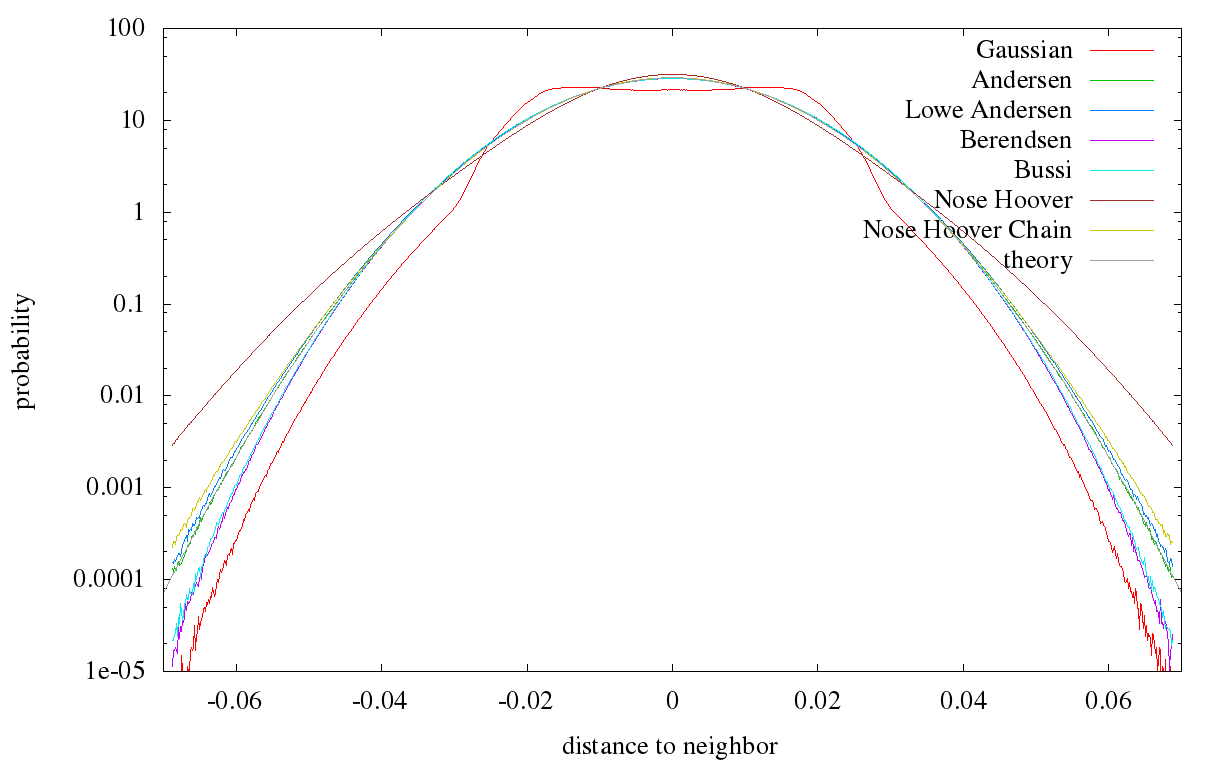
\includegraphics[width=0.9\textwidth]{./graphics/Histogramm_relPos_rand_T=20_p=64.png}
\caption{Histogram of $r_i - r_j$ for all thermostats}
\label{im:relPos_rand}
\end{figure} 
As can be seen in figure \ref{im:relPos_rand}, the Andersen, Lowe-Andersen and Nosé-Hoover Chain thermostats follow this probability distribution closely. The Nosé-Hoover thermostat exhibits a greater variance than expected, while the Berendsen and its relative, the Bussi-Donadio-Parrinello thermostat,  lead to a smaller variance. 

If we look at the distribution of particle velocities (figure \ref{im:vel_rand}), we see that the kinetic energy and the potential energy are strongly coupled in this system and the errors in the neighbour distance distribution probably arise from the errors in the distribution of velocities. The expected probability density is

\begin{equation}
f(v) = \left(\frac{m\beta}{2\pi p}\right)^{1/2}e^{-\frac{m\beta v^2}{2p}}
\end{equation} 
which is again only achieved by the Andersen, Lowe-Andersen and Nosé-Hoover Chain thermostats. 

\begin{figure}[H]
\centering
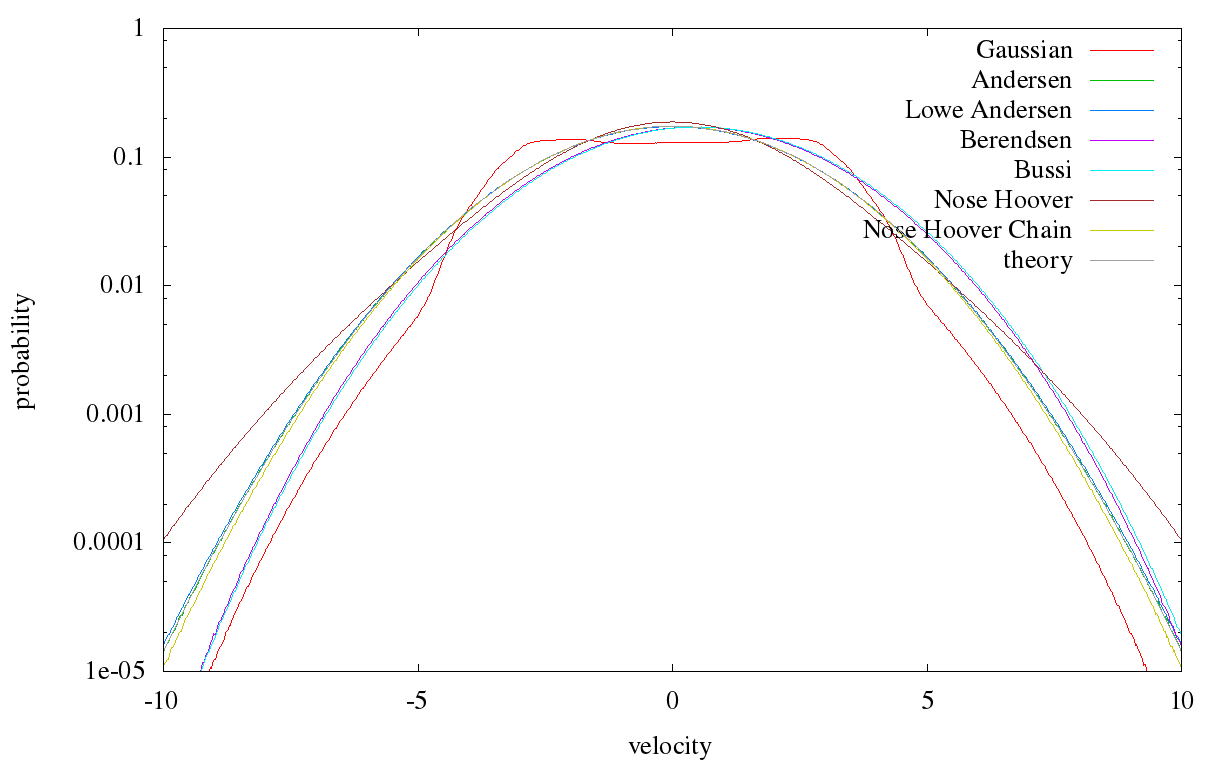
\includegraphics[width=0.9\textwidth]{./graphics/Histogramm_velocity_rand_T=20_p=64.png}
\caption{Histogram of particle velocities for all thermostats}
\label{im:vel_rand}
\end{figure}
To take a closer look at the thermostating routines, we also evaluated the distribution of the total kinetic energy of the polymer. Figure \ref{im:temp_rand} shows the distribution of virtual or instantaneous 'temperature' (i.e. $T' = 2E_{kin}/q$). The values obtained via the Nosé-Hoover algorithm deviate significantly from the theoretical probability distribution

\begin{equation}
f(T') = e^{-\frac{qT'}{2T}}\cdot \Gamma(q/2)^{-1}\cdot \left(\frac{qT'}{2T}\right)^{\frac{q}{2}}\frac{1}{T'}  
\end{equation}
and the maximum of the distribution does not coincide with the desired temperature. This is especially intriguing, because the distribution of the individual velocities (figure \ref{im:vel_rand}) deviated from the expected distribution to a far lesser extent. 
The Bussi-Donadio-Parinello thermostat, which should lead to a better distribution in kinetic energy than the Berendsen thermostat, because it incorporates stochastic fluctuations, exhibits the smallest variance in temperature of all thermostats - except for the Gaussian temperature of course, which, by construction, keeps the system always at the designated temperature and therefore the resulting ensemble is isokinetic rather than canonical.  

\begin{figure}[H]
\centering
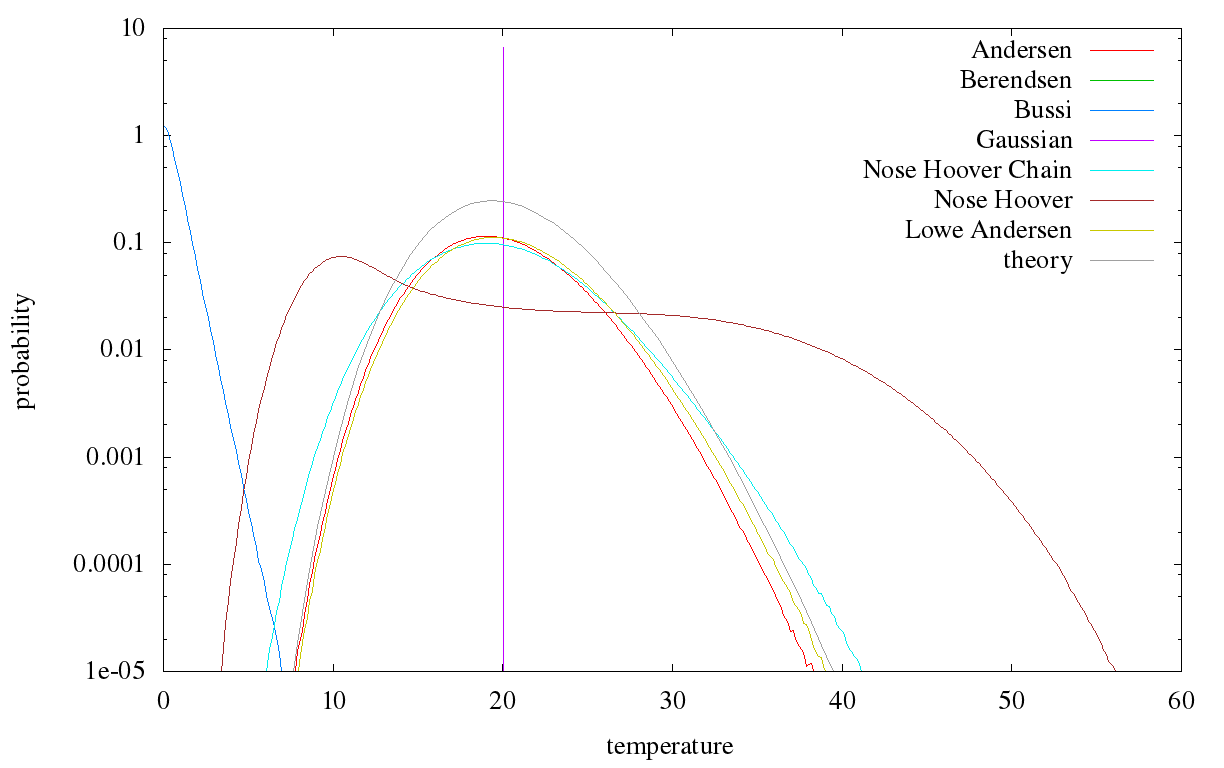
\includegraphics[width=0.9\textwidth]{./graphics/Histogramm_tempCol_rand_T=20_p=64.png}
\caption{Histogram of virtual temperature for all thermostats}
\label{im:temp_rand}
\end{figure}

\begin{figure}[H]
\centering
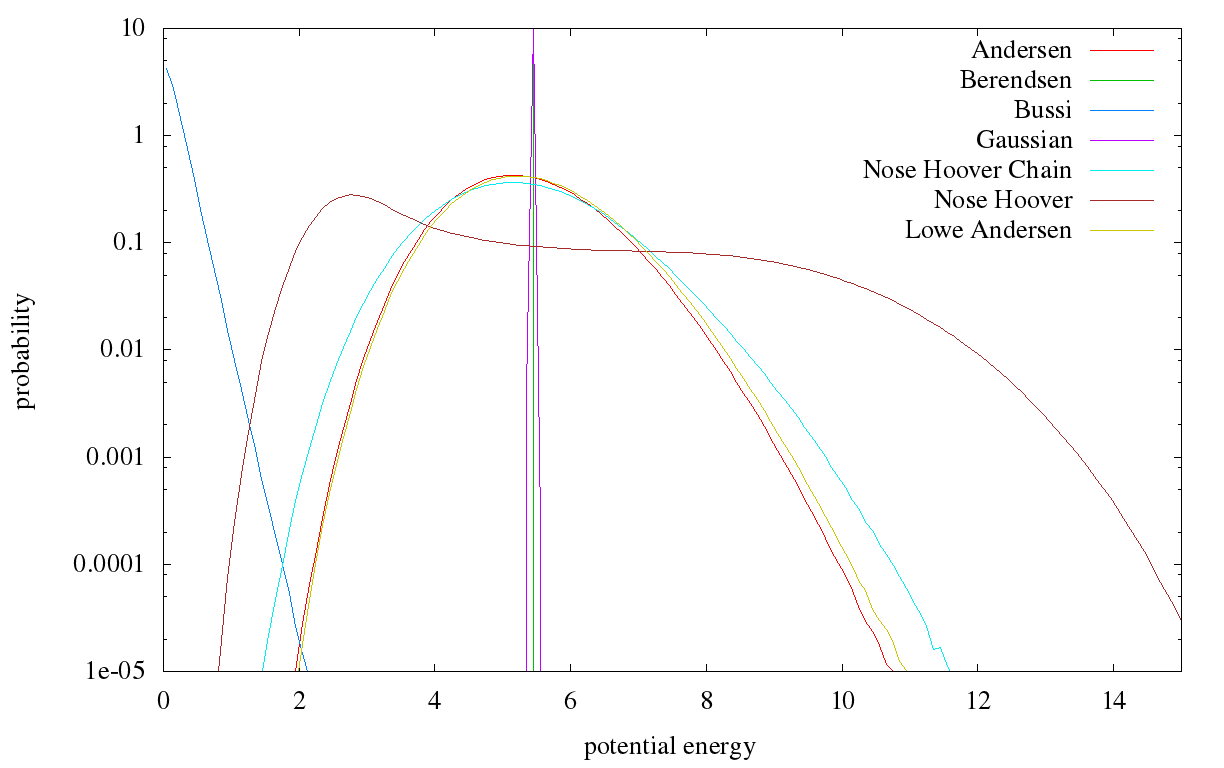
\includegraphics[width=0.9\textwidth]{./graphics/Histogramm_epot_rand_T=20_p=64.png}
\caption{Histogram of potential energy for all thermostats}
\label{im:epot_rand}
\end{figure}
In figure \ref{im:epot_rand} we can see the strong coupling between potential energy and kinetic energy in this system. Interesting to note here is, that the Andersen, Lowe--Anders, Nosé--Hoover--Chain and Gaussian thermostats share approximately the same maximum in potential energy - even though they exhibit different variances -, while the maximum is shifted to a higher value for the Bussi--Donadio--Parinello thermostat and the Nosé--Hoover thermostat leads to a highly asymmetric distribution of potential energy, for which we have not found a satisfying explanation.    

To detect other possible problems, we also looked at the distribution of monomer positions and the center of mass position (figures \ref{im:absPos_rand} and \ref{im:schwerPos_rand}). Ideally, the center of mass should not move at all, since its velocity was set to zero at the time of initialisation. However, in the Andersen method the center of mass velocity is not conserved due to the stochastic changes in the monomer velocities. The Lowe-Andersen method overcomes this problem by acting on relative velocities rather than absolute velocities, which leaves the total momentum invariant. 

Sometimes, changes in total momentum can happen due to rounding errors in the integration scheme and this can lead to the so-called 'flying icecube' phenomenon - i.e. the whole system moves with a constant center-of-mass velocity. Such behaviour can be seen for the Berendsen and Bussi-Donadio-Parinello thermostats in fig \ref{im:schwerVel_one}. A good thermostating routine should be able to dampen such effects.
\begin{figure}[H]
    \centering
    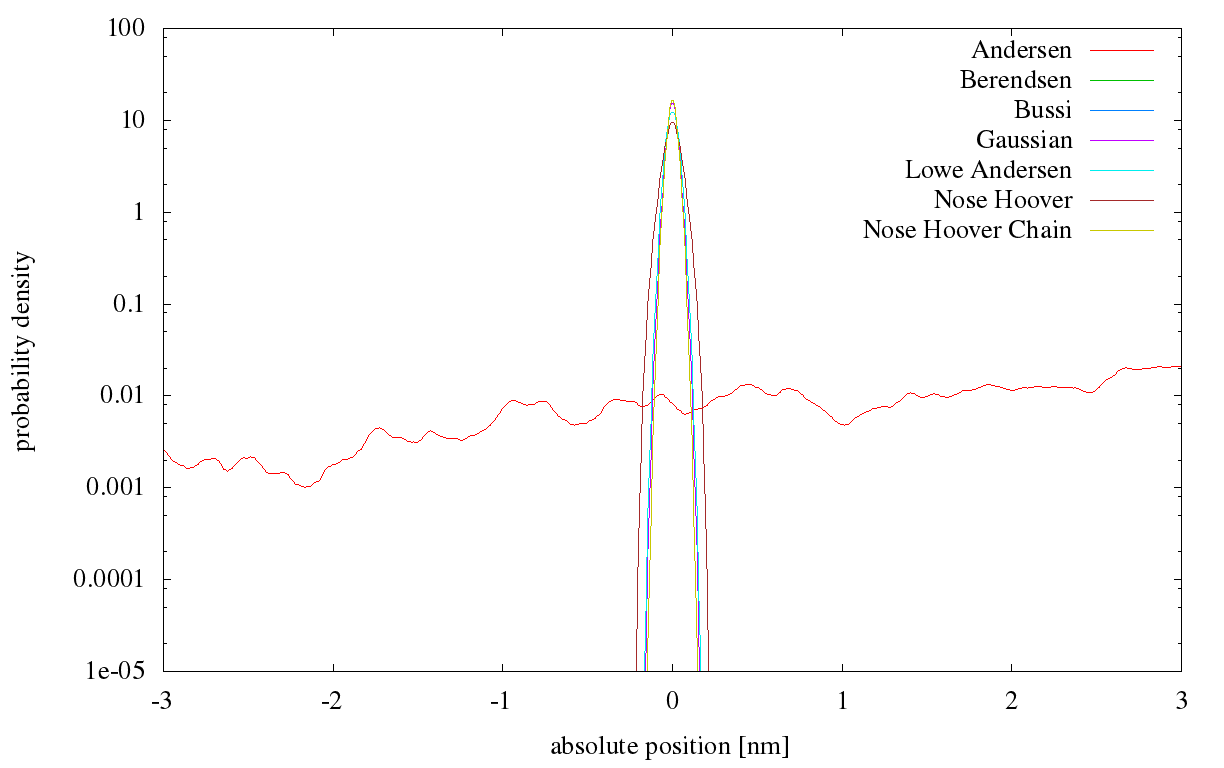
\includegraphics[width=0.9\textwidth]{./graphics/Histogramm_absPosition_rand_T=20_p=64.png}
  	\caption{Histogram of positions $r_i$}
    \label{im:absPos_rand}
\end{figure}

\begin{figure}[H]
    \centering
    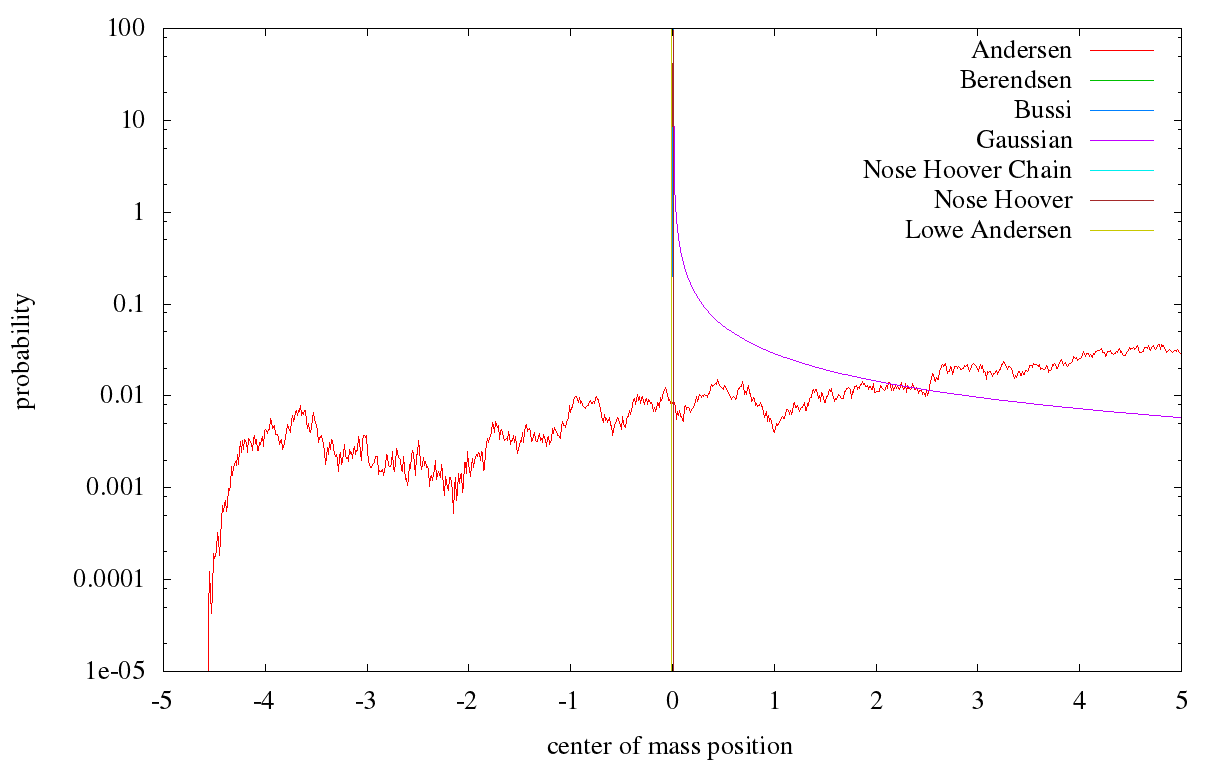
\includegraphics[width=0.9\textwidth]{./graphics/Histogramm_schwerPos_rand_T=20_p=64.png}
    \caption{Histogram of center of mass positions}
    \label{im:schwerPos_rand}
\end{figure}

\begin{figure}[H]
\centering
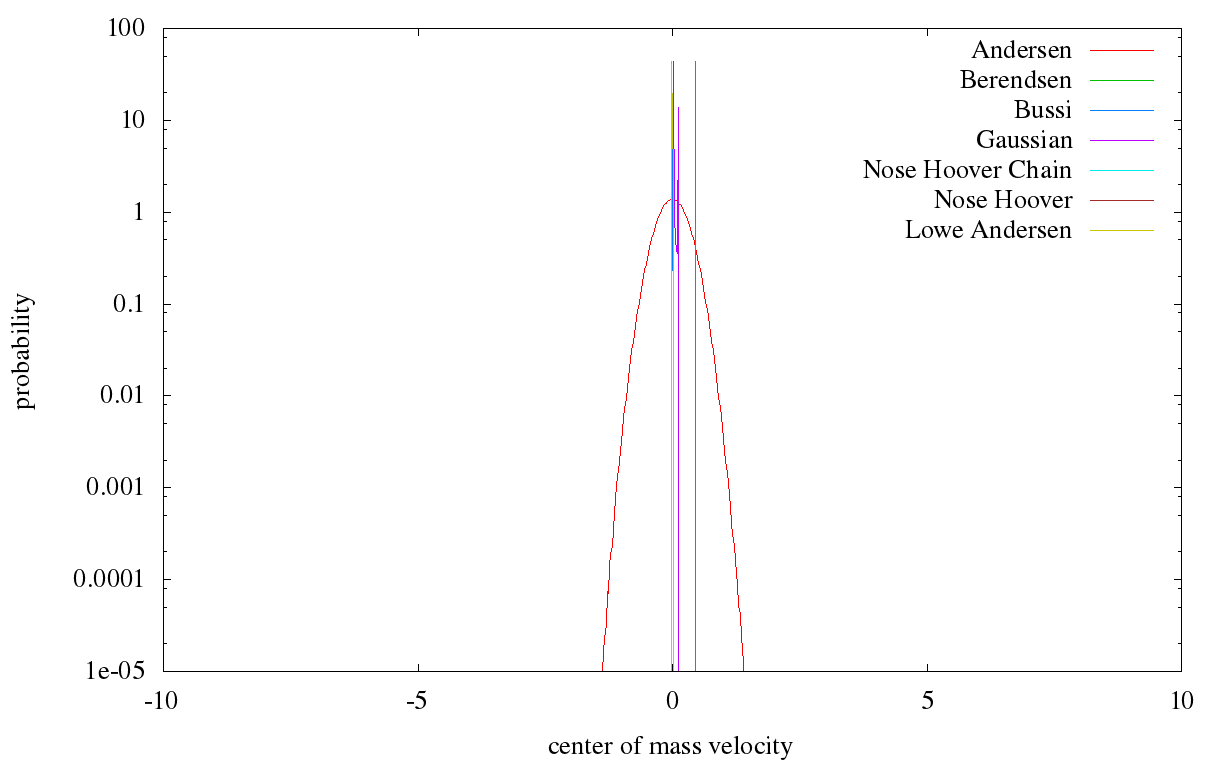
\includegraphics[width=0.9\textwidth]{./graphics/Histogramm_schwerVel_rand_T=20_p=64.png}
\caption{Histogram of center of mass velocities for all thermostats}
\label{im:schwerVel_rand}
\end{figure} 

\newpage
\subsection{Biased initialization}
Simulations started with our biased initialization method, which was introduced in section \ref{implementation}, were in general more prone to errors, and helped us to uncover more difficulties with the different thermostats. 

\begin{figure}[H]
\centering
  	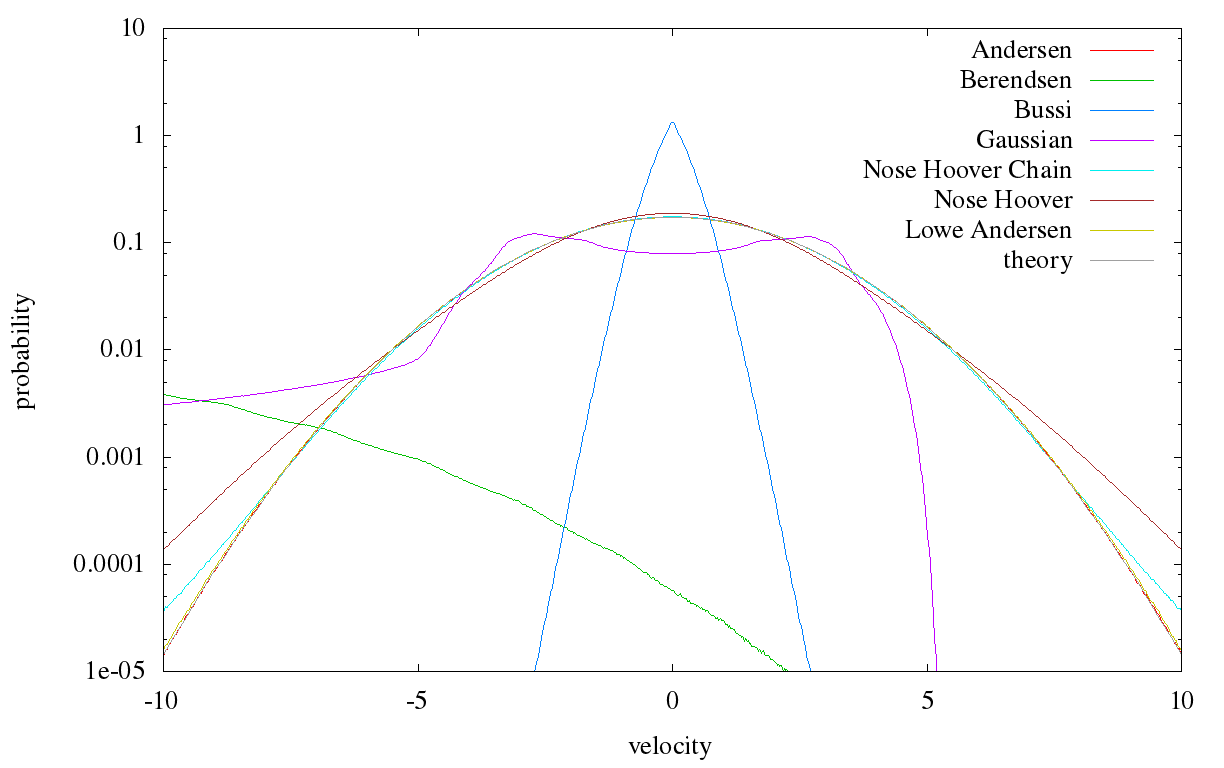
\includegraphics[width=0.9\textwidth]{./graphics/Histogramm_velocity_one_T=20_p=64.png}
  	\caption{Histogram of particle velocities for all thermostats}
    \label{im:vel_one}
\end{figure} 


\begin{figure}[H]
\centering
    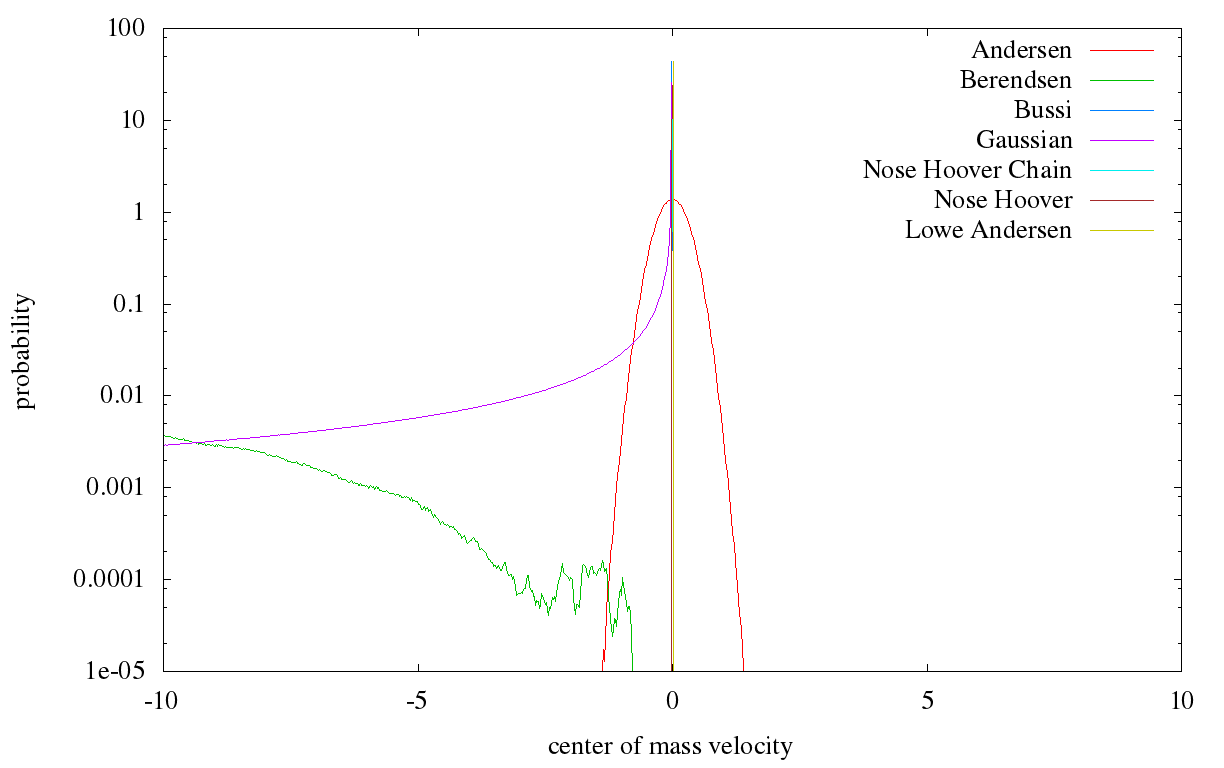
\includegraphics[width=0.9\textwidth]{./graphics/Histogramm_schwerVel_one_T=20_p=64.png}
    \caption{Histogram of center of mass velocities for all thermostats}
    \label{im:schwerVel_one} 
\end{figure} 
As can be seen from figure \ref{im:vel_one} and \ref{im:schwerVel_one}, the systems thermostated using the Berendsen and Bussi-Donadio-Parinello methods experienced an acceleration of center of mass velocity, which could not be counteracted by the thermostats. This is responsible for the discontinuous histogram in figure \ref{im:relPos_one}, since the absolute positions grew so large that the precision of double floating point numbers was not high enough to resolve the distances $r_i - r_j$ correctly (Please note that the distributions for the Berendsen and the Bussi--Donadio--Parinello  thermostats overlap).

\begin{figure}[H]
\centering
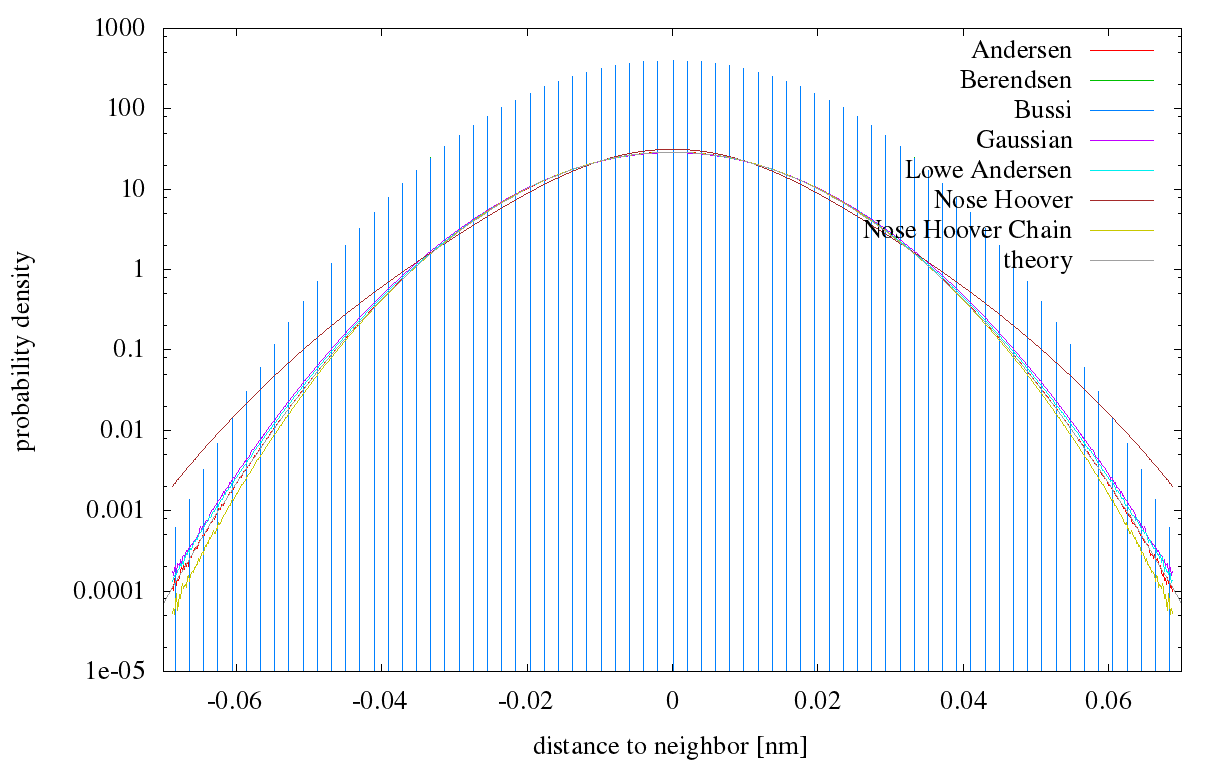
\includegraphics[width=0.9\textwidth]{./graphics/Histogramm_relPos_one_T=20_p=64.png}
\caption{Histogram of $r_i - r_j$ for all thermostats}
\label{im:relPos_one}
\end{figure} 

Finally, we noticed that the Bussi-Donadio-Parinello thermostat exhibits a better distribution in instantaneous temperature $T'$ if the system is initialized with the biased initialisation method (see figure \ref{im:temp_one}). We have not yet found a satisfying explanation for this behaviour. 


\begin{figure}[H]
\centering
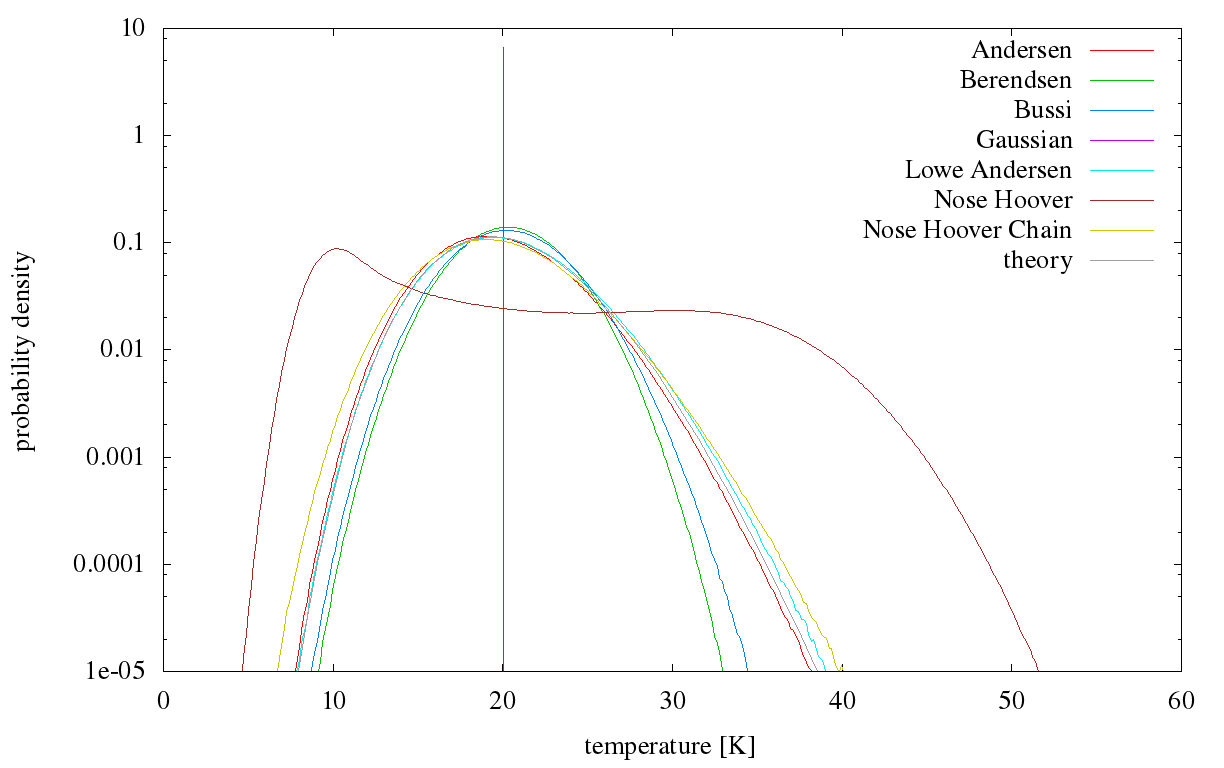
\includegraphics[width=0.9\textwidth]{./graphics/Histogramm_tempCol_one_T=20_p=64.png}
\caption{Histogram of instantaneous temperature for all thermostats}
\label{im:temp_one}
\end{figure}

\begin{comment}
\begin{figure}[H]
\centering
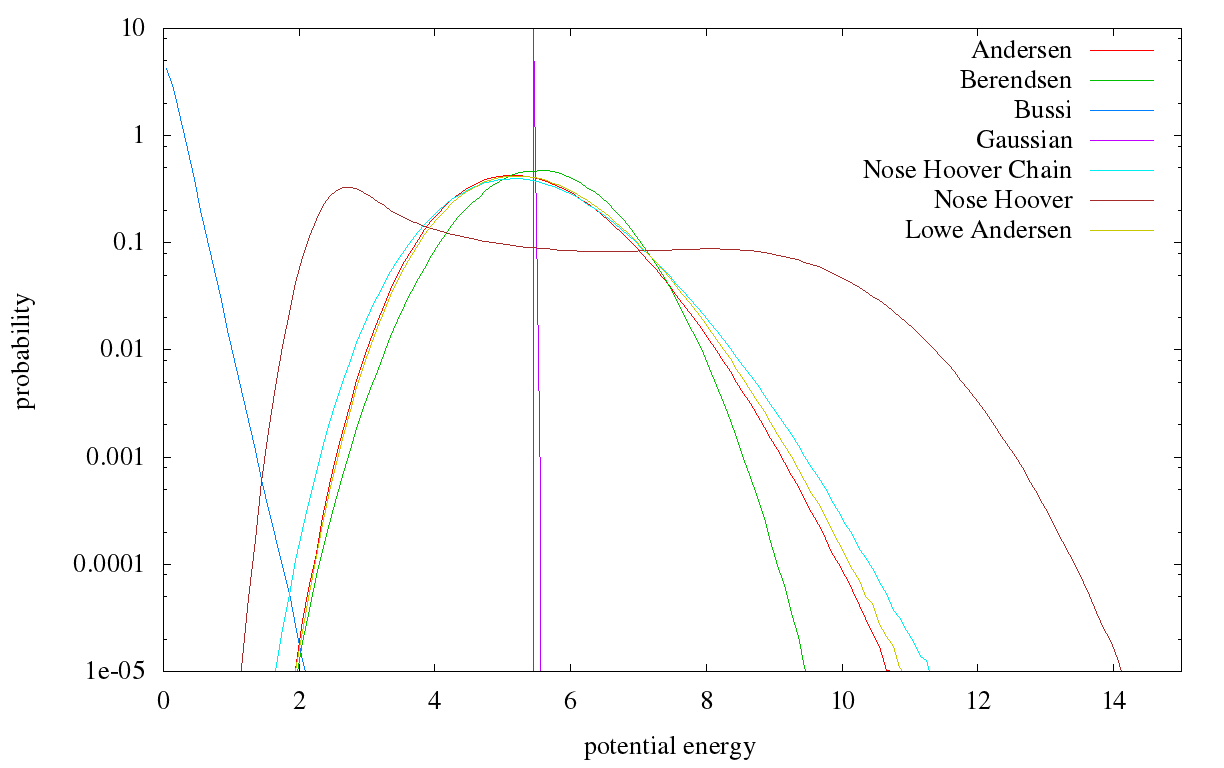
\includegraphics[width=0.9\textwidth]{./graphics/Histogramm_epot_one_T=20_p=64.png}
\caption{Histogram of potential energy for all thermostats}
\label{im:epot_one}
\end{figure}

\begin{figure}[H]
\centering
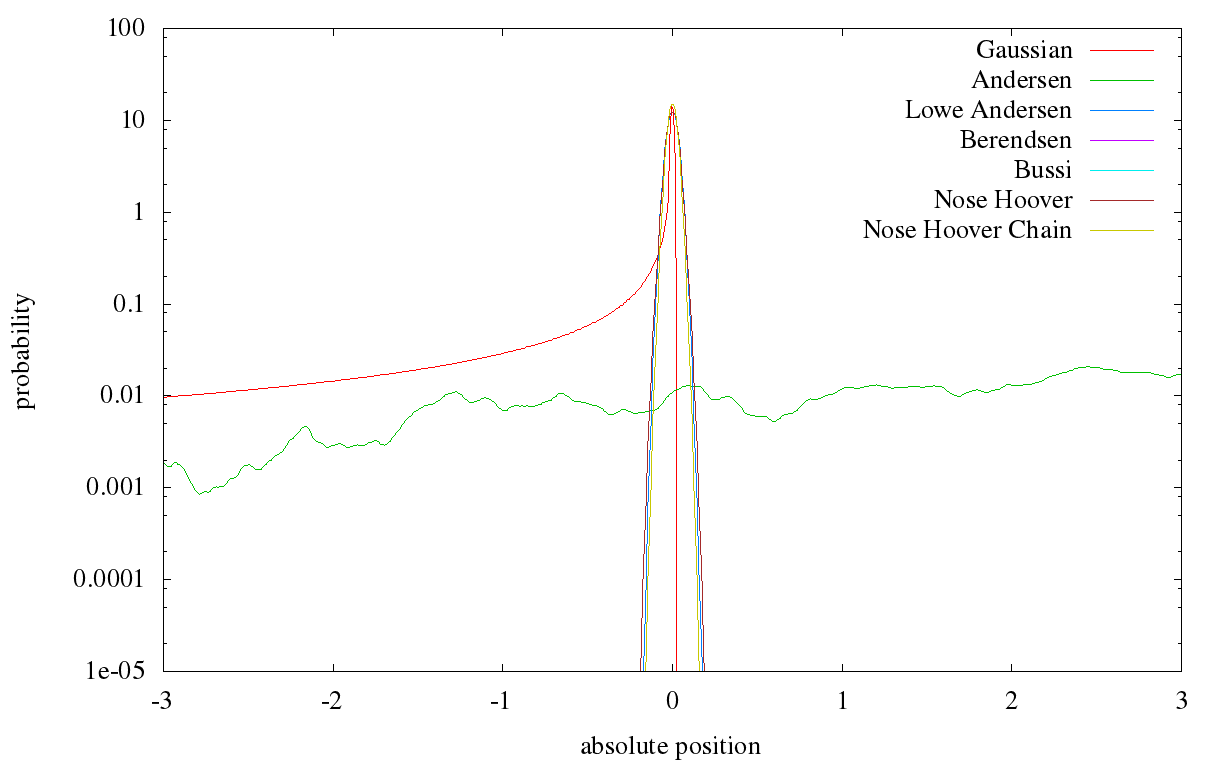
\includegraphics[width=0.9\textwidth]{./graphics/Histogramm_absPosition_one_T=20_p=64.png}
\caption{Histogram of positions $r_i$ for all thermostats}
\label{im:absPos_one}
\end{figure} 

\begin{figure}[H]
\centering
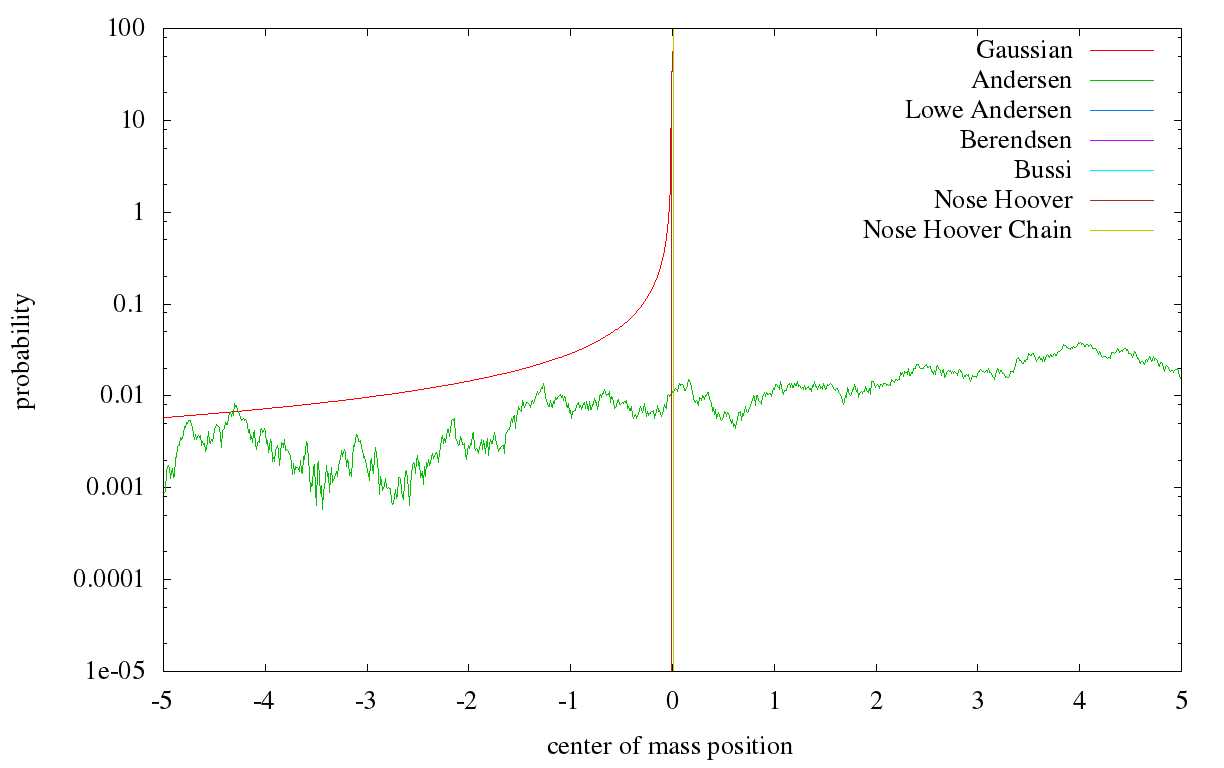
\includegraphics[width=0.9\textwidth]{./graphics/Histogramm_schwerPos_one_T=20_p=64.png}
\caption{Histogram of center of mass positions for all thermostats}
\label{im:schwerPos_one}
\end{figure} 

\end{comment}

\subsection{Parameters for the thermostats}
\subsubsection{Berendsen \& Bussi--Donadio--Parrinello}
The change rate $\tau$ is the only free parameter in both thermostats---it controls by how much the kinetic energies are scaled in one time step. We used 
\begin{equation}
\tau = 10\cdot \Delta t = 10fs\text{.}
\end{equation}

\subsubsection{Nosé--Hoover Chain}
The Nosé-Hoover thermostat includes a freely choosable parameter $Q$ (or $Q_1$ and $Q_2$ for the Nosé-Hoover Chain), which controls the strength of coupling to the heat bath. As mentioned in section \ref{NHC}, Martyna \textit{et al.} \cite{Martyna1992} suggest using $Q_1 = \frac{qkT}{\omega}$ and $Q_j = \frac{kT}{\omega}$, where $\omega$ is a typical frequency of the system. In our project, we also used these parameters at first with $\omega$ being the frequency of harmonic oscillations resulting from the spring potential.
\begin{equation}
\omega = \sqrt{\frac{k}{m}} = \frac{q}{\beta \hbar}
\end{equation} 
where $k$ is the spring constant. In our reduced units, we arrived at values of 
\begin{align*}
& Q_1 = 0.063528 \text{kJ}/(\text{mol ps}) && Q_2 \approx 0.001
\end{align*} 
However, to test this suggestion and to make sure we got the best results possible, we varied $Q_2$ over several orders of magnitude while keeping $Q_1 = q\cdot Q_2$. Figure \ref{im:temp_chain} shows the probability distributions of instantaneous temperature for different values of $Q_2$. We found that a strong coupling - i.e. small $Q_2$ - leads to the best agreement with the theoretical distribution for a canonical ensemble. For comparing the different thermostats (section \ref{results}), the results from the simulation with $Q_2 = 0.001$ and $Q_1 = 0.064$ were used. 

\begin{figure}[H]
\centering
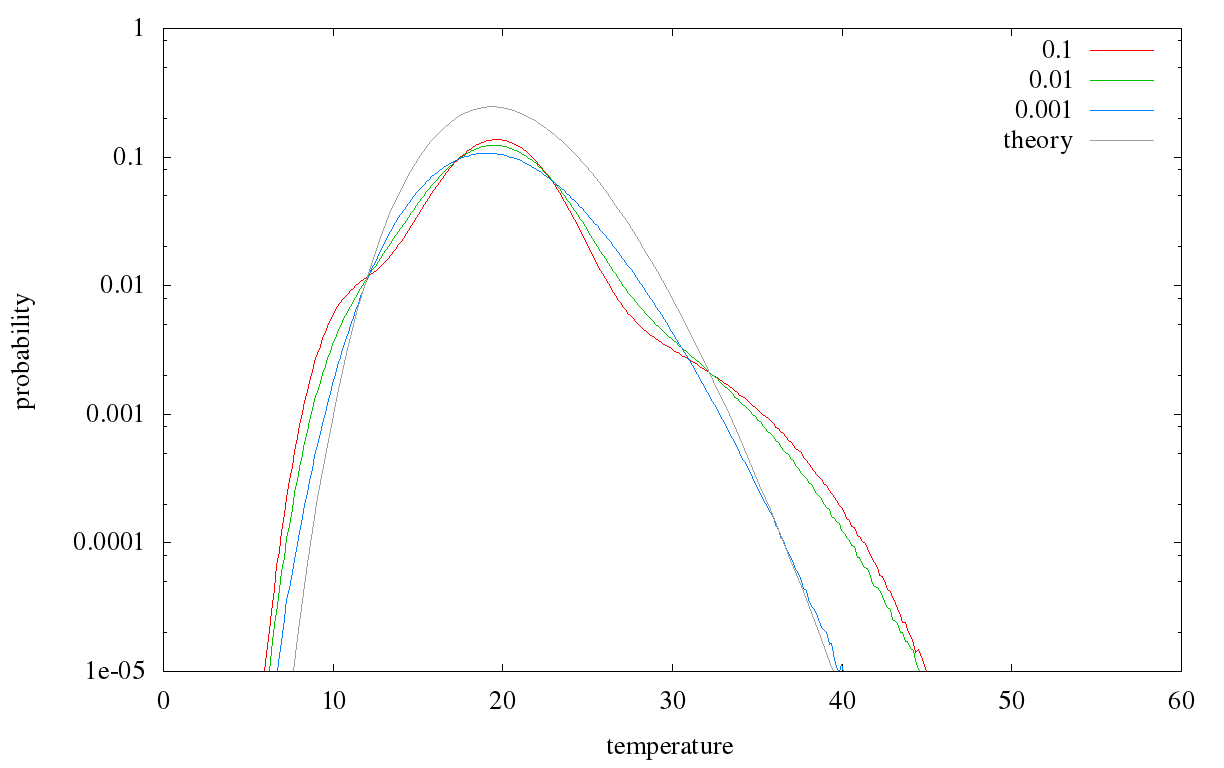
\includegraphics[width=0.9\textwidth]{./graphics/Histogramm_tempCol_one_Chain.png}
\caption{Histogram of instantaneous temperature of the Nose Hoover Chain for different values of $Q_2$ }
\label{im:temp_chain}
\end{figure}



